\documentclass[a4paper,11pt,notitlepage]{report}

\usepackage[utf8]{inputenc}
\DeclareUnicodeCharacter{251C}{|--}
\DeclareUnicodeCharacter{2502}{|}
\DeclareUnicodeCharacter{2514}{`--}
\DeclareUnicodeCharacter{2500}{-}
\usepackage[T1]{fontenc}
\usepackage{amsmath}
\usepackage{amsthm}
\usepackage{amssymb}
\usepackage{enumerate}
\usepackage{graphicx}
\usepackage[vmargin=2.6cm,hmargin=2.9cm]{geometry}
\usepackage{indentfirst}
\usepackage{cite}
\usepackage[frenchb,french]{babel}
\usepackage{eurosym}
\usepackage{algorithm}
\usepackage{algorithmic}
\usepackage{textcomp}
\usepackage{hyperref}
\usepackage{subcaption}
\usepackage{pdfpages}
\usepackage{qrcode}
\usepackage{listings}
\usepackage{xcolor}
\usepackage{fancyhdr}
\usepackage{float}

\interfootnotelinepenalty=10000

\lstdefinestyle{bash}{
  language=bash,
  backgroundcolor=\color{gray!10},
  basicstyle=\ttfamily\small,
  keywordstyle=\color{black},
  commentstyle=\color{green!60!black},
  stringstyle=\color{orange},
  frame=single,
  rulecolor=\color{gray!50},
  breaklines=true,
  showstringspaces=false,
}

\lstdefinestyle{tree}{
  backgroundcolor=\color{gray!10},
  basicstyle=\ttfamily\small,
  frame=single,
  rulecolor=\color{gray!50},
  breaklines=false,
  showstringspaces=false,
}

\setlength{\marginparwidth}{2cm}
\raggedbottom

\usepackage{todonotes}
% \usepackage[disable]{todonotes}

\usepackage{pslatex}

\renewcommand{\labelitemi}{--}


\graphicspath{ {images/} }

\floatname{algorithm}{Algorithme}
\renewcommand{\algorithmicrequire}{\textbf{Entrée:}}
\renewcommand{\algorithmicensure}{\textbf{Sortie:}}
\renewcommand{\algorithmicif}{\textbf{si}}
\renewcommand{\algorithmicthen}{\textbf{alors}}
\renewcommand{\algorithmicelse}{\textbf{sinon}}
\renewcommand{\algorithmicfor}{\textbf{pour}}
\renewcommand{\algorithmicend}{\textbf{fin}}
\renewcommand{\algorithmicdo}{\textbf{faire}}


\pagestyle{fancy}
\fancyhf{} % vide en-têtes et pieds de page
\fancyhead[L]{\nouppercase{\leftmark}} % titre du chapitre à gauche
\fancyhead[R]{\thepage} % numéro de page à droite
\renewcommand{\headrulewidth}{0.4pt}

\newcommand{\STitre}{UNIVERSITÉ DE MONS}
\newcommand{\FTitre}{FACULTÉ DES SCIENCES UMONS}
\newcommand{\Titre}{Reconstruction 3D des mouvements de force athlétique à partir de vidéos monoculaires.}


\renewcommand{\O}{\mathcal{O}}
\newtheorem{thm}{Théorème}
\newtheorem{cor}{Corollaire}
\newtheorem{conj}{Conjecture}
\newtheorem{lem}{Lemme}
\newtheorem{prop}{Proposition}
\newtheorem{exa}{Exemple}
\newtheorem{rem}{Remarque}
\theoremstyle{definition}
\newtheorem{defn}{Définition}


\newenvironment{compar}{
\begin{center}
  \begin{quote}
    \sf \small
    \begin{tabular}{p{0.4\textwidth} | p{0.4\textwidth}}
      }{
    \end{tabular}
  \end{quote}
\end{center}
\rm \normalsize
}


\def\signed #1{{\leavevmode\unskip\nobreak\hfil\penalty50\hskip2em
\hbox{}\nobreak\hfil(#1)%
\parfillskip=0pt \finalhyphendemerits=0 \endgraf}}

\newsavebox\mybox
\newenvironment{aquote}[1]
{\savebox\mybox{#1}
\begin{quote}
  }
  {\signed{\usebox\mybox}
\end{quote}
}


%\title{\LARGE\bf \Titre}


\title{
\begin{minipage}
  \linewidth\centering 
  \LARGE\bf\STitre
  \vskip20pt 
  \Large\bf\FTitre
  \vskip20pt 
  \Huge \Titre    
\end{minipage}
}

\author{Nicolas DELPLANQUE\\[1.5ex]
Master en Sciences Informatiques\\[1.5ex]
{\tt \small nicolas.delplanque@student.umons.ac.be}
}
\date{Année académique 2025-2026}
\begin{document}


\maketitle
\smallskip



\markright{\Titre}


\thispagestyle{empty}

\bigskip

%\renewcommand{\contentsname}{Contenu}

\vfill

\begin{quote}
  {Mémoire présenté en vue de l'obtention du grade académique de {\bf Master en Sciences Informatiques}  \\ } 

\end{quote}
\begin{quote}
  {\centering \bf Service : } Service d'Intelligence Artificielle \\
  {\centering \bf Directeur : } Stéphane DUPONT \\
  %%{\centering \bf Co-directeur : } Bruno QUOITIN
\end{quote}

\vfill


\includegraphics[width=0.2\textwidth]{FS} \hspace{0.6\textwidth} 
\includegraphics[width=0.2\textwidth]{logo_UMONS} \hspace{0.2\textwidth} 

\newpage
\thispagestyle{empty}
L'auteur, DELPLANQUE Nicolas, atteste avoir respecté les règles éthiques en vigueur, y compris la charte de l'Université relative à l'utilisation de l'Intelligence Artificielle. 

% cfr. Règlement mémoires ...

\newpage
\thispagestyle{empty}

\section*{Remerciements} \label{sec_rem}

Je tiens à exprimer ma profonde gratitude envers toutes les personnes qui ont rendu ce travail possible.

À mon directeur de mémoire, Stéphane Dupont, pour son accompagnement, ses conseils avisés et la confiance qu'il m'a accordée tout au long de ce travail.

À mes parents, sans qui ce parcours n'aurait pas été possible. Leur soutien indéfectible et les nombreux sacrifices qu'ils ont consentis pour me permettre de poursuivre mes ambitions sont un cadeau dont je mesure aujourd'hui toute la valeur.

À mon frère Alexandre, d'avoir pris le temps de relire ce travail avec attention. Tes retours m'ont été d'une grande aide.

À ma copine Sarah, pour ta relecture soigneuse et, plus encore, pour ton soutien de chaque instant tout au long de ce parcours. Dans les moments de doute, lorsque l'envie d'abandonner se faisait sentir, tu as toujours su trouver les mots justes pour me redonner confiance et m'encourager à continuer. Tu as été un véritable pilier, et ce mémoire doit beaucoup à ta présence.

À mon coach et ami Nello, qui m'accompagne depuis plus de trois ans dans la pratique de la force athlétique. C'est lui qui m'a fait découvrir ce sport exigeant et c'est cet engagement partagé qui a inspiré le sujet de ce mémoire.

Enfin, je remercie l'ensemble des pratiquants volontaires qui ont accepté de partager leurs vidéos d'entraînement pour constituer le jeu de données, ainsi que tous mes proches pour leur soutien et leurs encouragements durant la réalisation de ce travail.

% \newpage
% \thispagestyle{empty}
% \mbox{}
% \newpage

\newpage
\tableofcontents
\normalsize

\newpage
% \thispagestyle{empty}
% \mbox{}
% \newpage



\setlength{\parindent}{12pt}
\setlength{\parskip}{1ex plus 0.5ex minus 0.2ex}

% ---------------------
% INTRODUCTION
% ---------------------
\chapter{Introduction} \label{ch_one}

L'optimisation de la performance sportive exige une quantification rigoureuse des paramètres posturaux~\cite{Colyer-2018}. Traditionnellement réservé aux environnements de laboratoire équipés de capteurs intrusifs~\cite{Colyer-2018}, l'évaluation biomécanique connaît une mutation fondamentale sous l'impulsion de la vision par ordinateur et de l'apprentissage profond (\textit{deep learning})~\cite{Human-Pose-Estimation-2021}. Ce mémoire étudie l'intégration de ces architectures, spécifiquement la segmentation sémantique \footnote{La segmentation sémantique (\textit{semantic segmentation}) désigne la tâche consistant à attribuer à chaque pixel d'une image une étiquette de classe (par exemple : personne, sol, équipement), produisant une partition de la scène en régions. Elle se distingue de la segmentation d'instances, qui différencie en outre les occurrences individuelles d'une même classe.}, la diffusion pour la complétion amodale \footnote{La complétion amodale (\textit{amodal completion}) désigne la capacité à reconstruire la forme complète d'un objet ou d'un sujet au-delà de sa seule partie visible, en inférant les régions masquées par une occlusion. Contrairement à l'\textit{inpainting classique} qui reconstruit le fond derrière un objet retiré, la complétion amodale cherche à restituer fidèlement la structure de l'objet ou du sujet partiellement caché, en s'appuyant sur les indices visuels disponibles et sur la connaissance apprise de la morphologie de l'objet ou du sujet.} et l'estimation de pose tridimensionnelle, appliquées à la force athlétique. L'intention première est la conception d'un pipeline d'analyse non invasif, capable d'extraire la pose d'un individu à partir de vidéos monoculaires non calibrés \footnote{Une vidéo monoculaire désigne une séquence captée par une unique caméra, par opposition aux systèmes stéréoscopiques ou multicaméras. Le qualificatif \emph{non calibrée} indique que les paramètres de la caméra (longueur focale, distorsion, centre optique) ne sont pas connus a priori, ce qui est le cas de la quasi-totalité des smartphones et caméras grand public.}. Ce premier chapitre définit le contexte, les enjeux, mais décrit aussi les défauts des méthodologies d'évaluation actuelles et structure les contributions technologiques développées au cours de ce mémoire.


\section{Contexte et enjeux de l'analyse biomécanique en force athlétique} \label{one_one}

La force athlétique est une discipline de compétition consistant en la réalisation de trois mouvements de base : la flexion de jambes (\textit{squat}), le développé couché (\textit{bench}) et le soulevé de terre (\textit{deadlift}).

{\large \textbf{Flexion de jambes}}

La flexion de jambes (figure~\ref{fig:squat}) est un mouvement au cours duquel l'athlète, barre chargée sur les épaules, doit descendre jusqu'à ce que la surface supérieure des cuisses passe en dessous du niveau des genoux, puis se relever jusqu'à la position droite. Le règlement technique de l'IPF (\textit{International Powerlifting Federation}) en donne la définition suivante :

"La barre sera maintenue horizontalement sur les épaules, mains et doigts la serrant. [...] le force-athlétiste doit fléchir les genoux et abaisser son corps jusqu'à ce que la surface supérieure des cuisses à l'articulation de la hanche soit plus basse que le sommet des genoux. [...] Le force-athlétiste doit se relever à sa guise jusqu'à une position droite, genoux verrouillés." \cite[p.~18]{IPF-Technical-Regulations-2025}

\begin{figure}
  [htp]
  \centering
  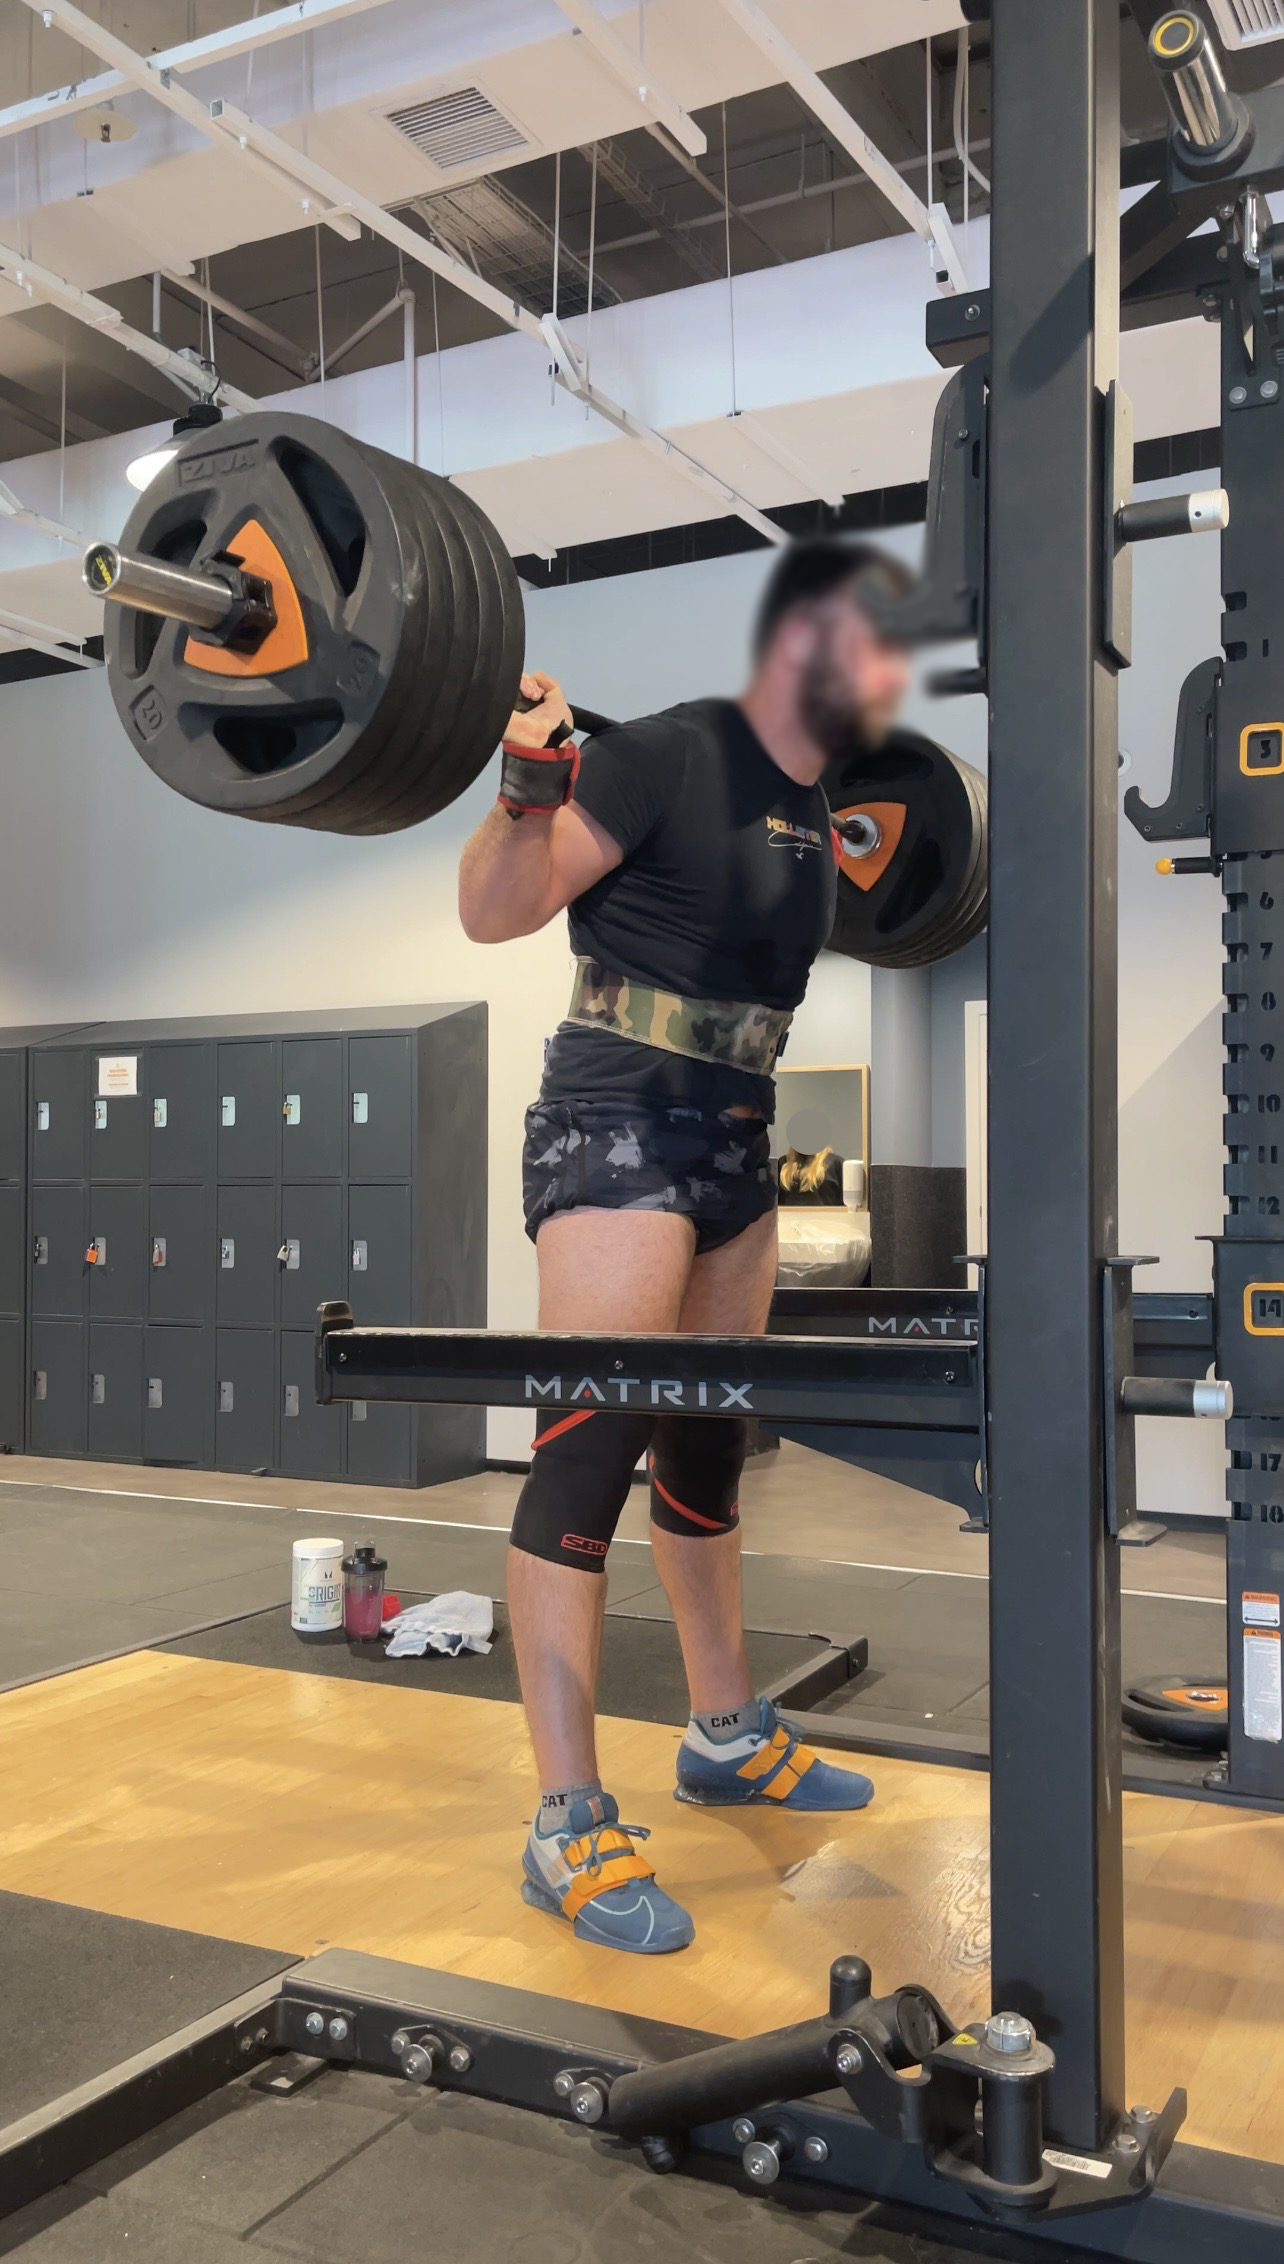
\includegraphics[width=3.5cm, height=5cm]{1-Introduction/1-Squat.jpg}
  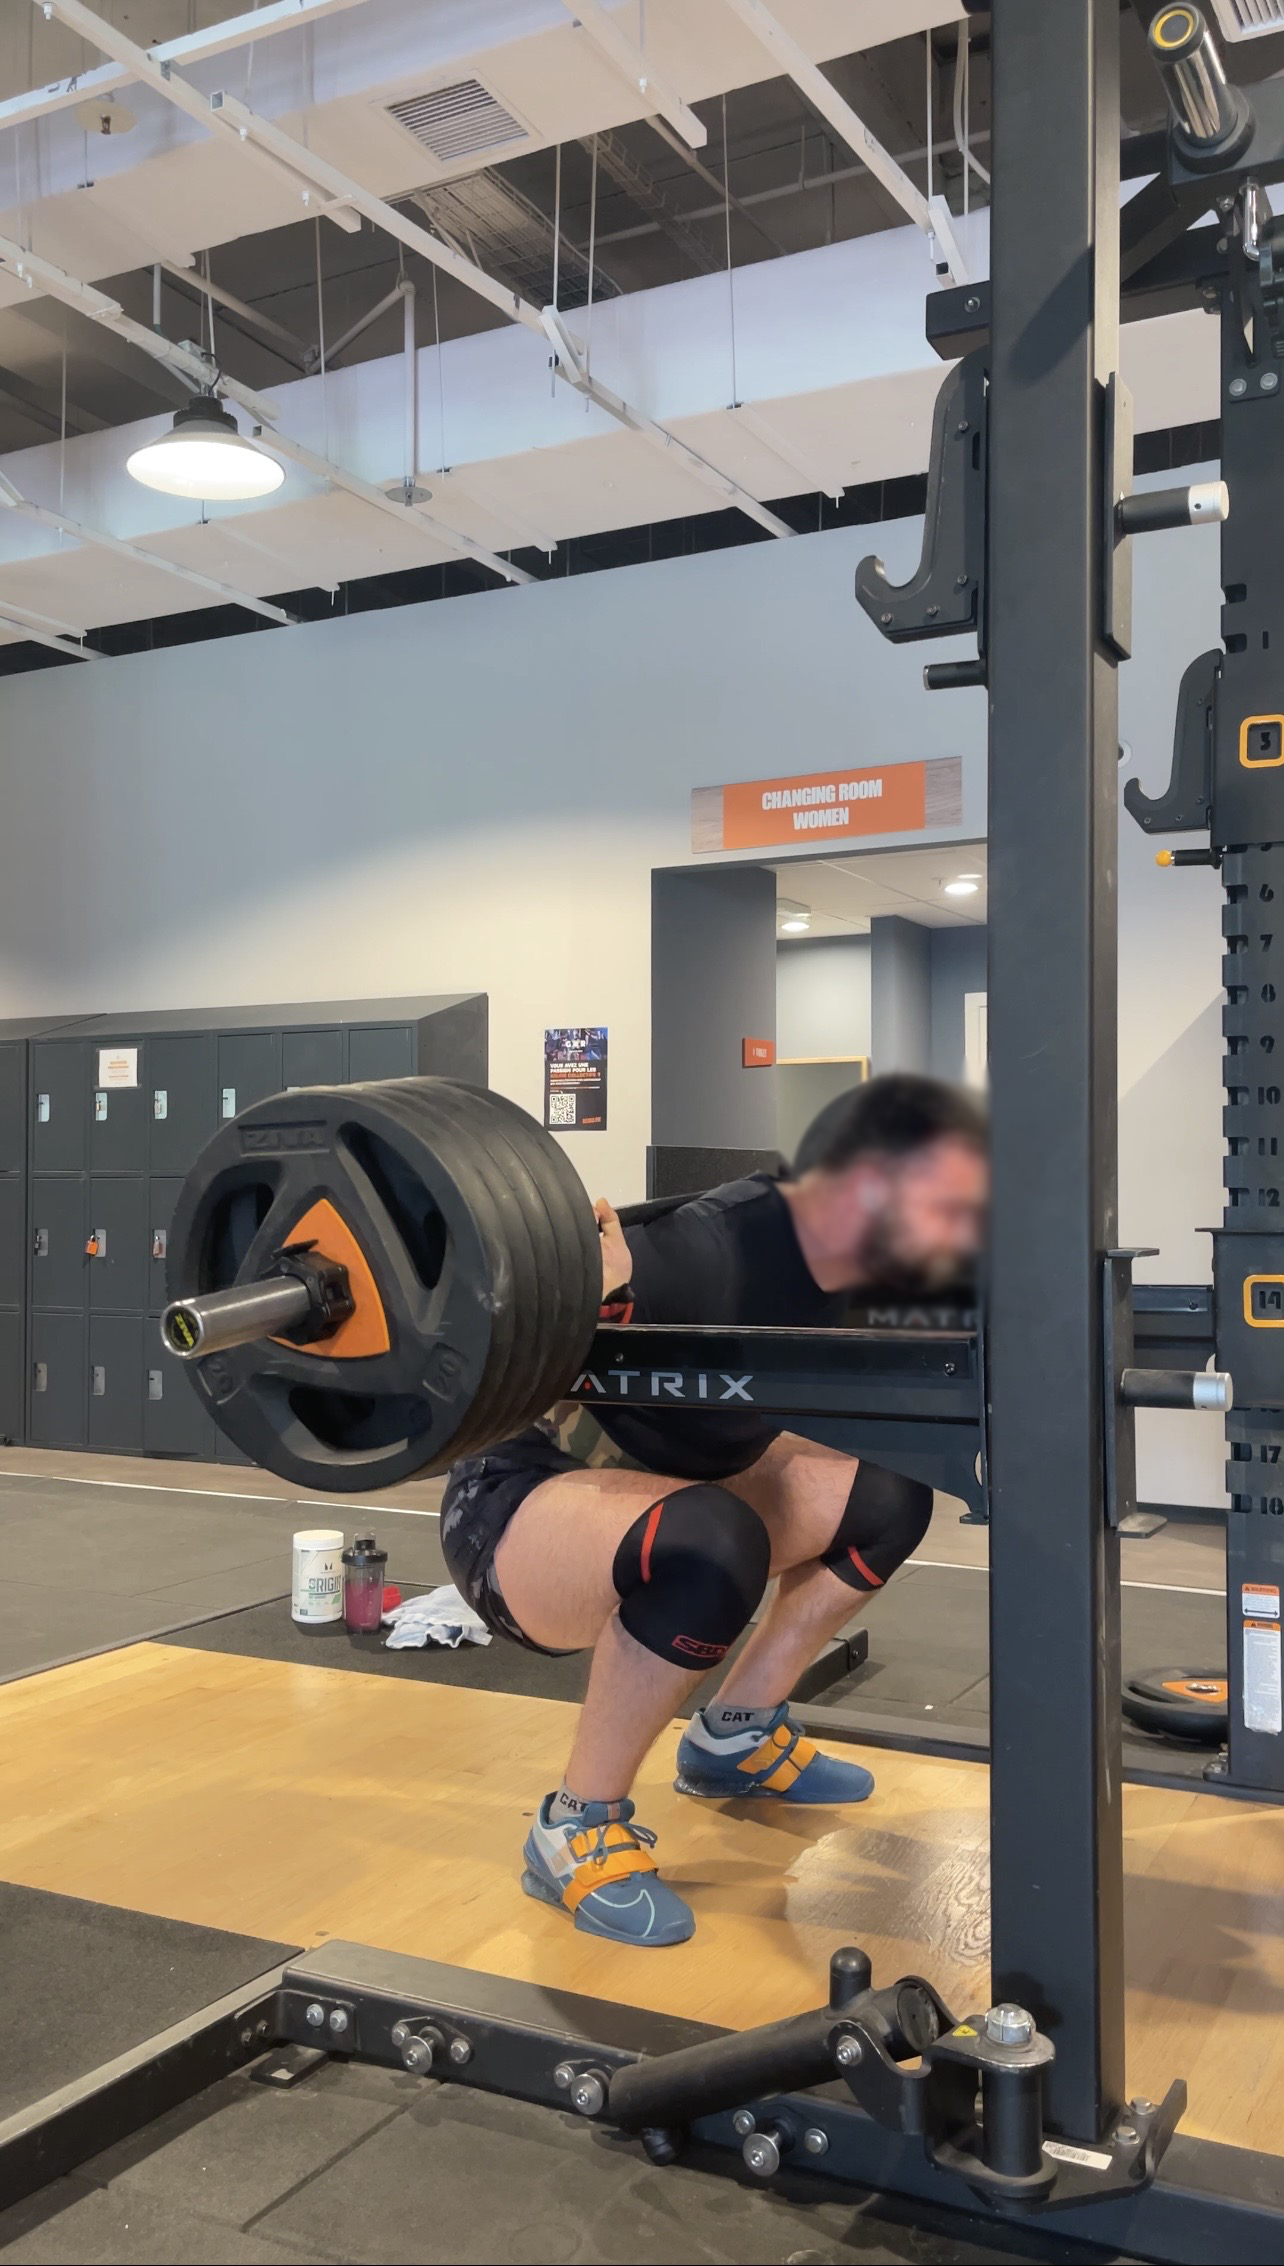
\includegraphics[width=3.5cm, height=5cm]{1-Introduction/2-Squat.jpg}
  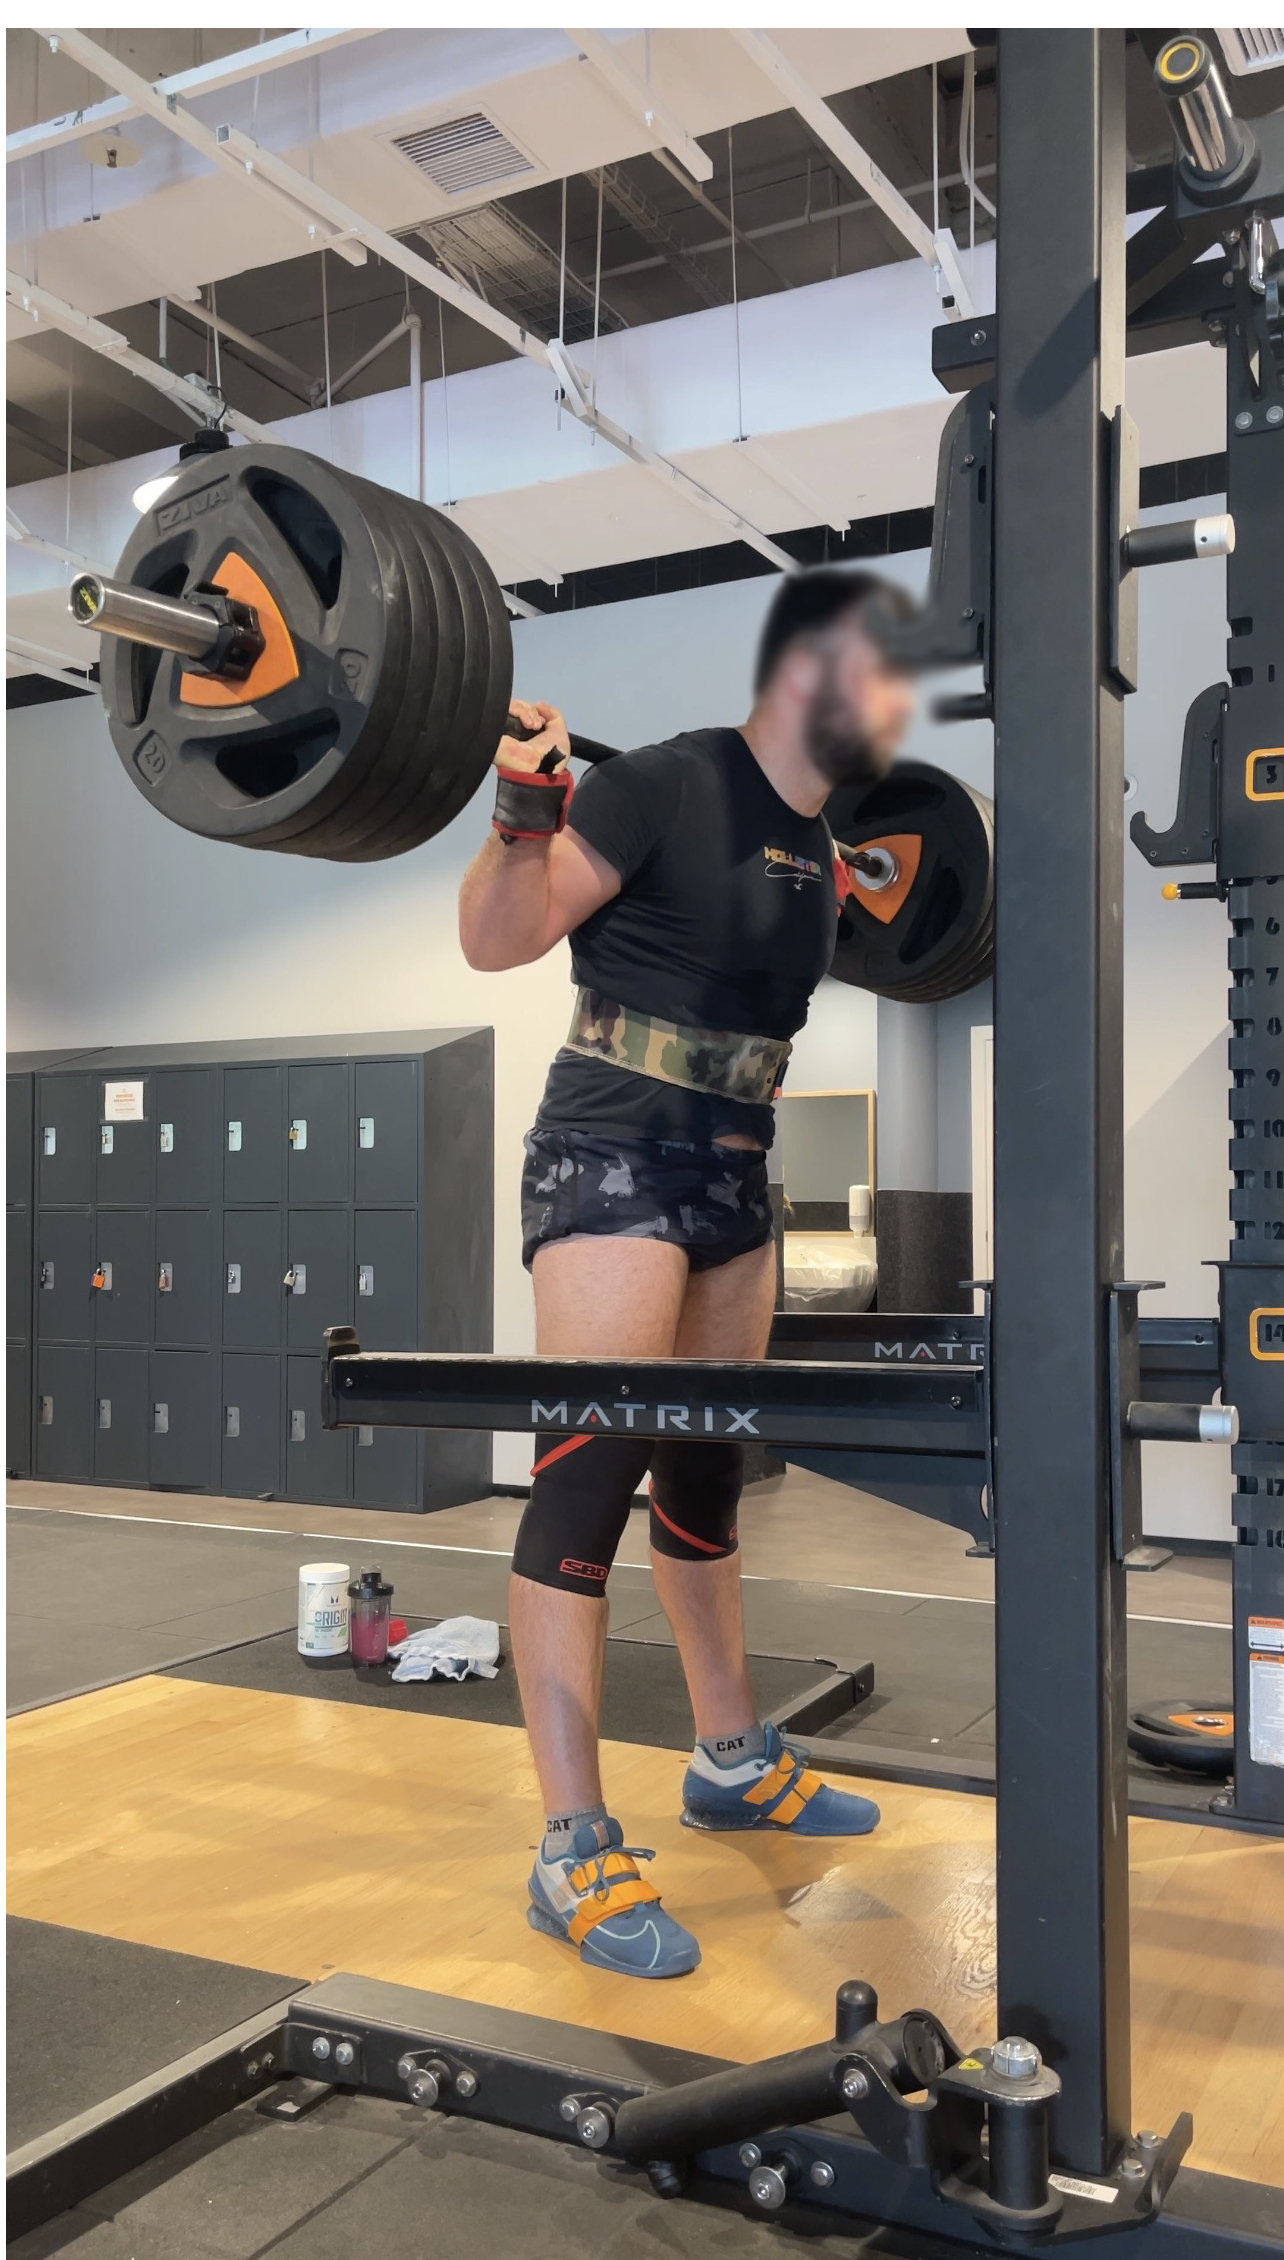
\includegraphics[width=3.5cm, height=5cm]{1-Introduction/3-Squat.jpg}
  \caption{Illustration d'une flexion de jambes}
  \label{fig:squat}
\end{figure}

{\large \textbf{Développé couché}}

Le développé couché (figure~\ref{fig:bench}) consiste, depuis une position allongée sur un banc, à descendre une barre chargée jusqu'au contact de la poitrine puis à la repousser jusqu'à l'extension complète des bras. Le règlement technique de l'IPF en donne la définition suivante :

"Le force-athlétiste doit s'allonger sur le dos de façon que sa tête, ses épaules et ses fessiers soient en contact avec la surface du banc [...]. Les pieds doivent être à plat sur le sol [...]. Ses mains et ses doigts doivent serrer la barre, [...] avec une prise pouces verrouillés. Cette position de corps doit être conservée pendant tout le mouvement. Les déplacements des pieds sont autorisés mais ils doivent rester sur le sol. [...] le force-athlétiste devra descendre la barre jusqu'au contact de la poitrine ou de la région abdominale et il doit avoir le dessous des articulations des coudes au-dessous ou au même niveau de la surface supérieure de l'articulation de leur épaule respective [...] le force-athlétiste doit ramener la barre au bout des bras tendus, en verrouillant les deux coudes." \cite[p.~18-19]{IPF-Technical-Regulations-2025} 

\begin{figure}
  [htp]
  \centering
  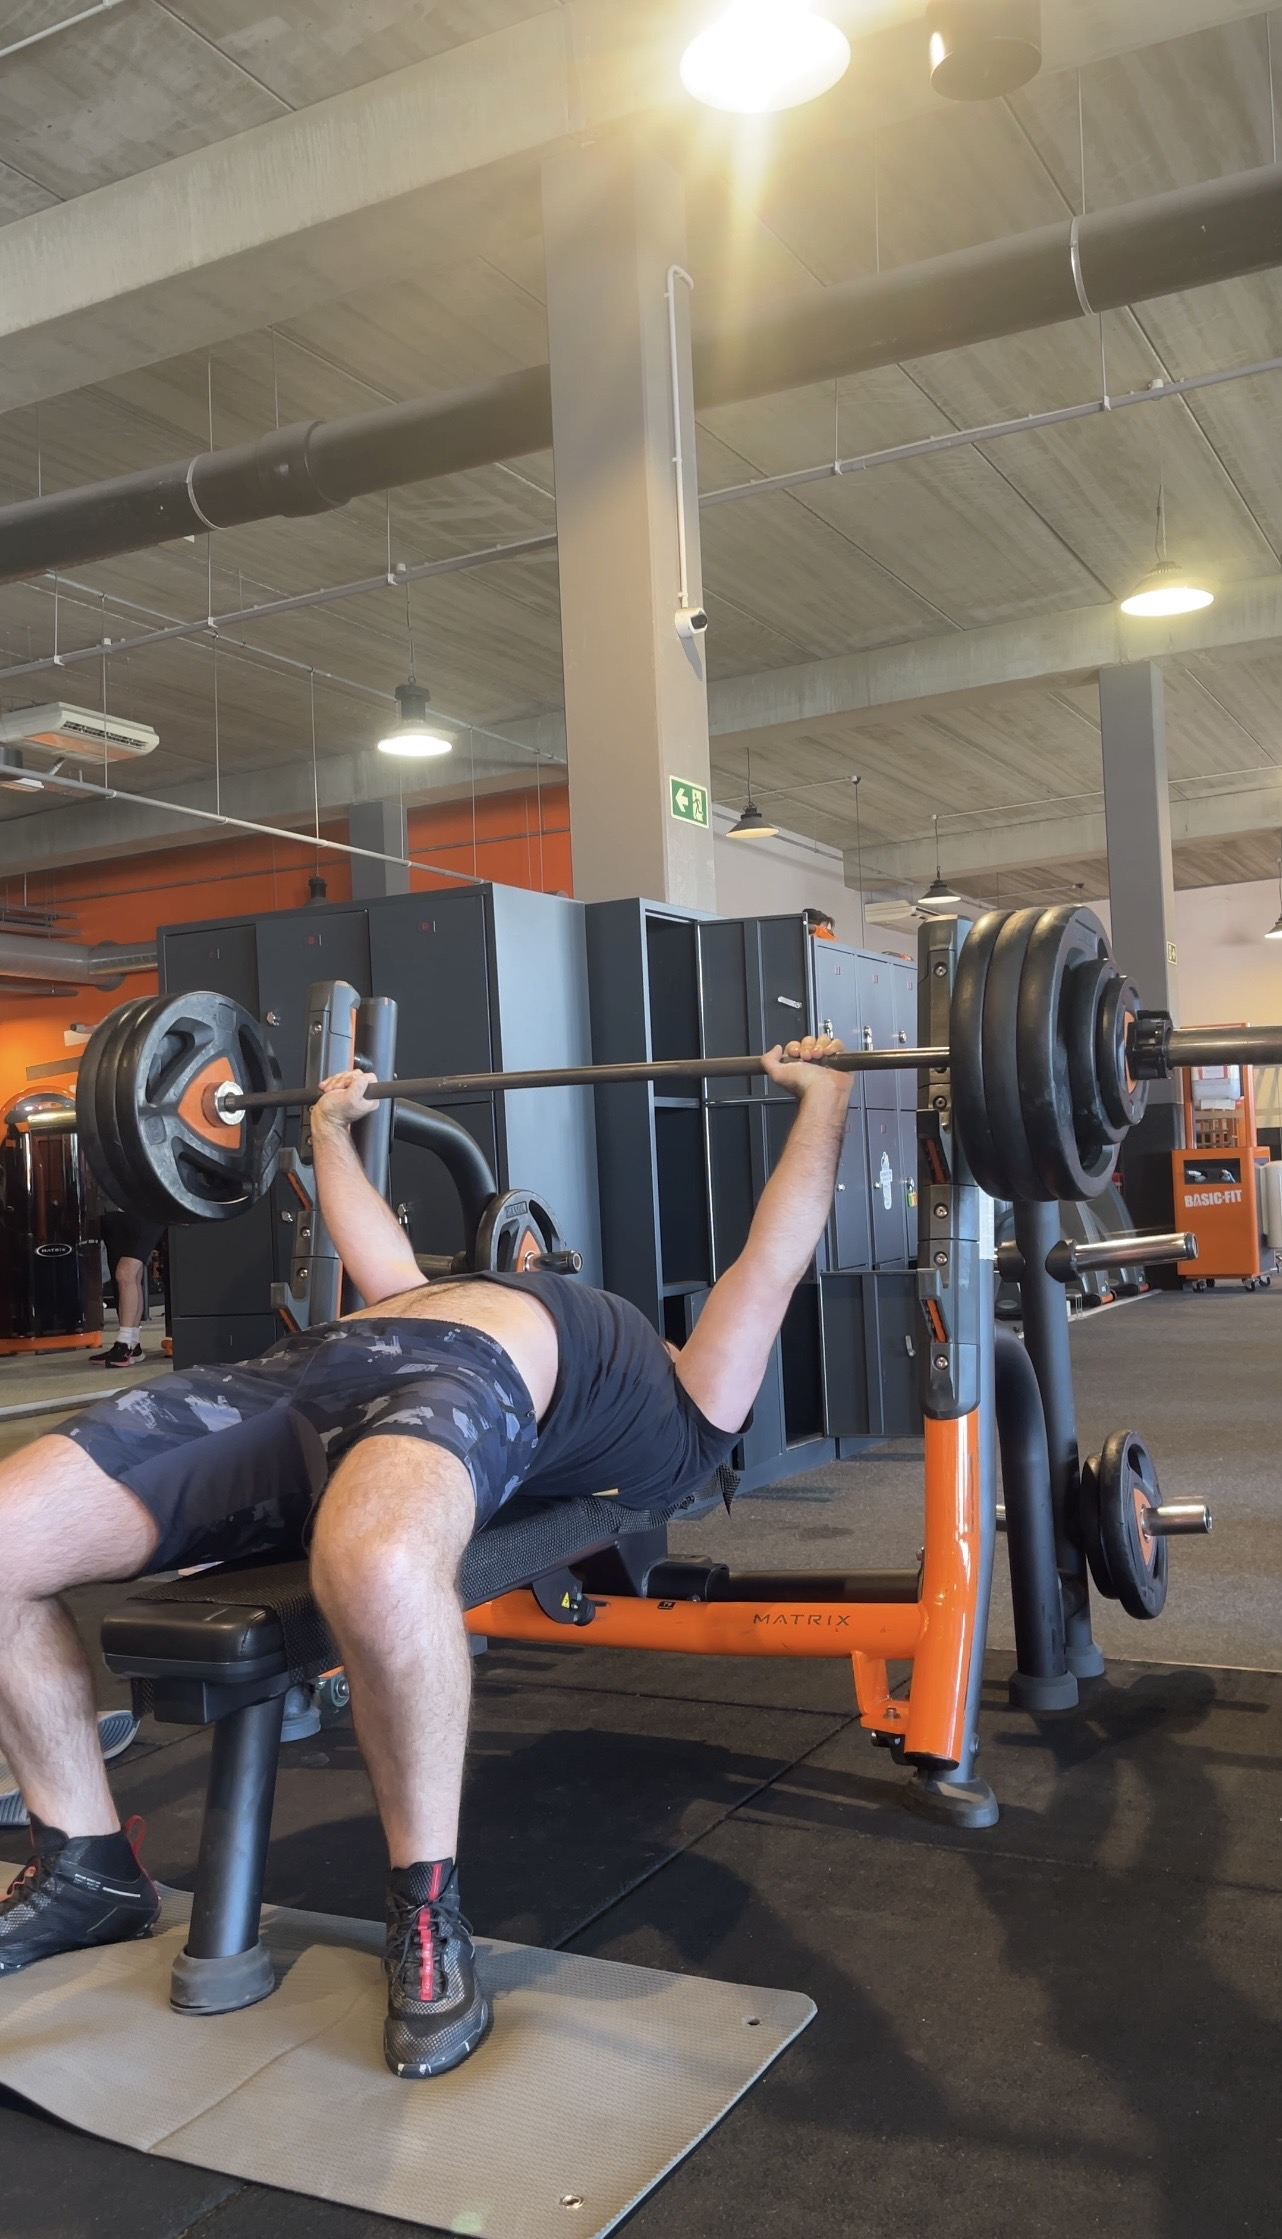
\includegraphics[width=3.5cm, height=5cm]{1-Introduction/1-Bench.jpg}
  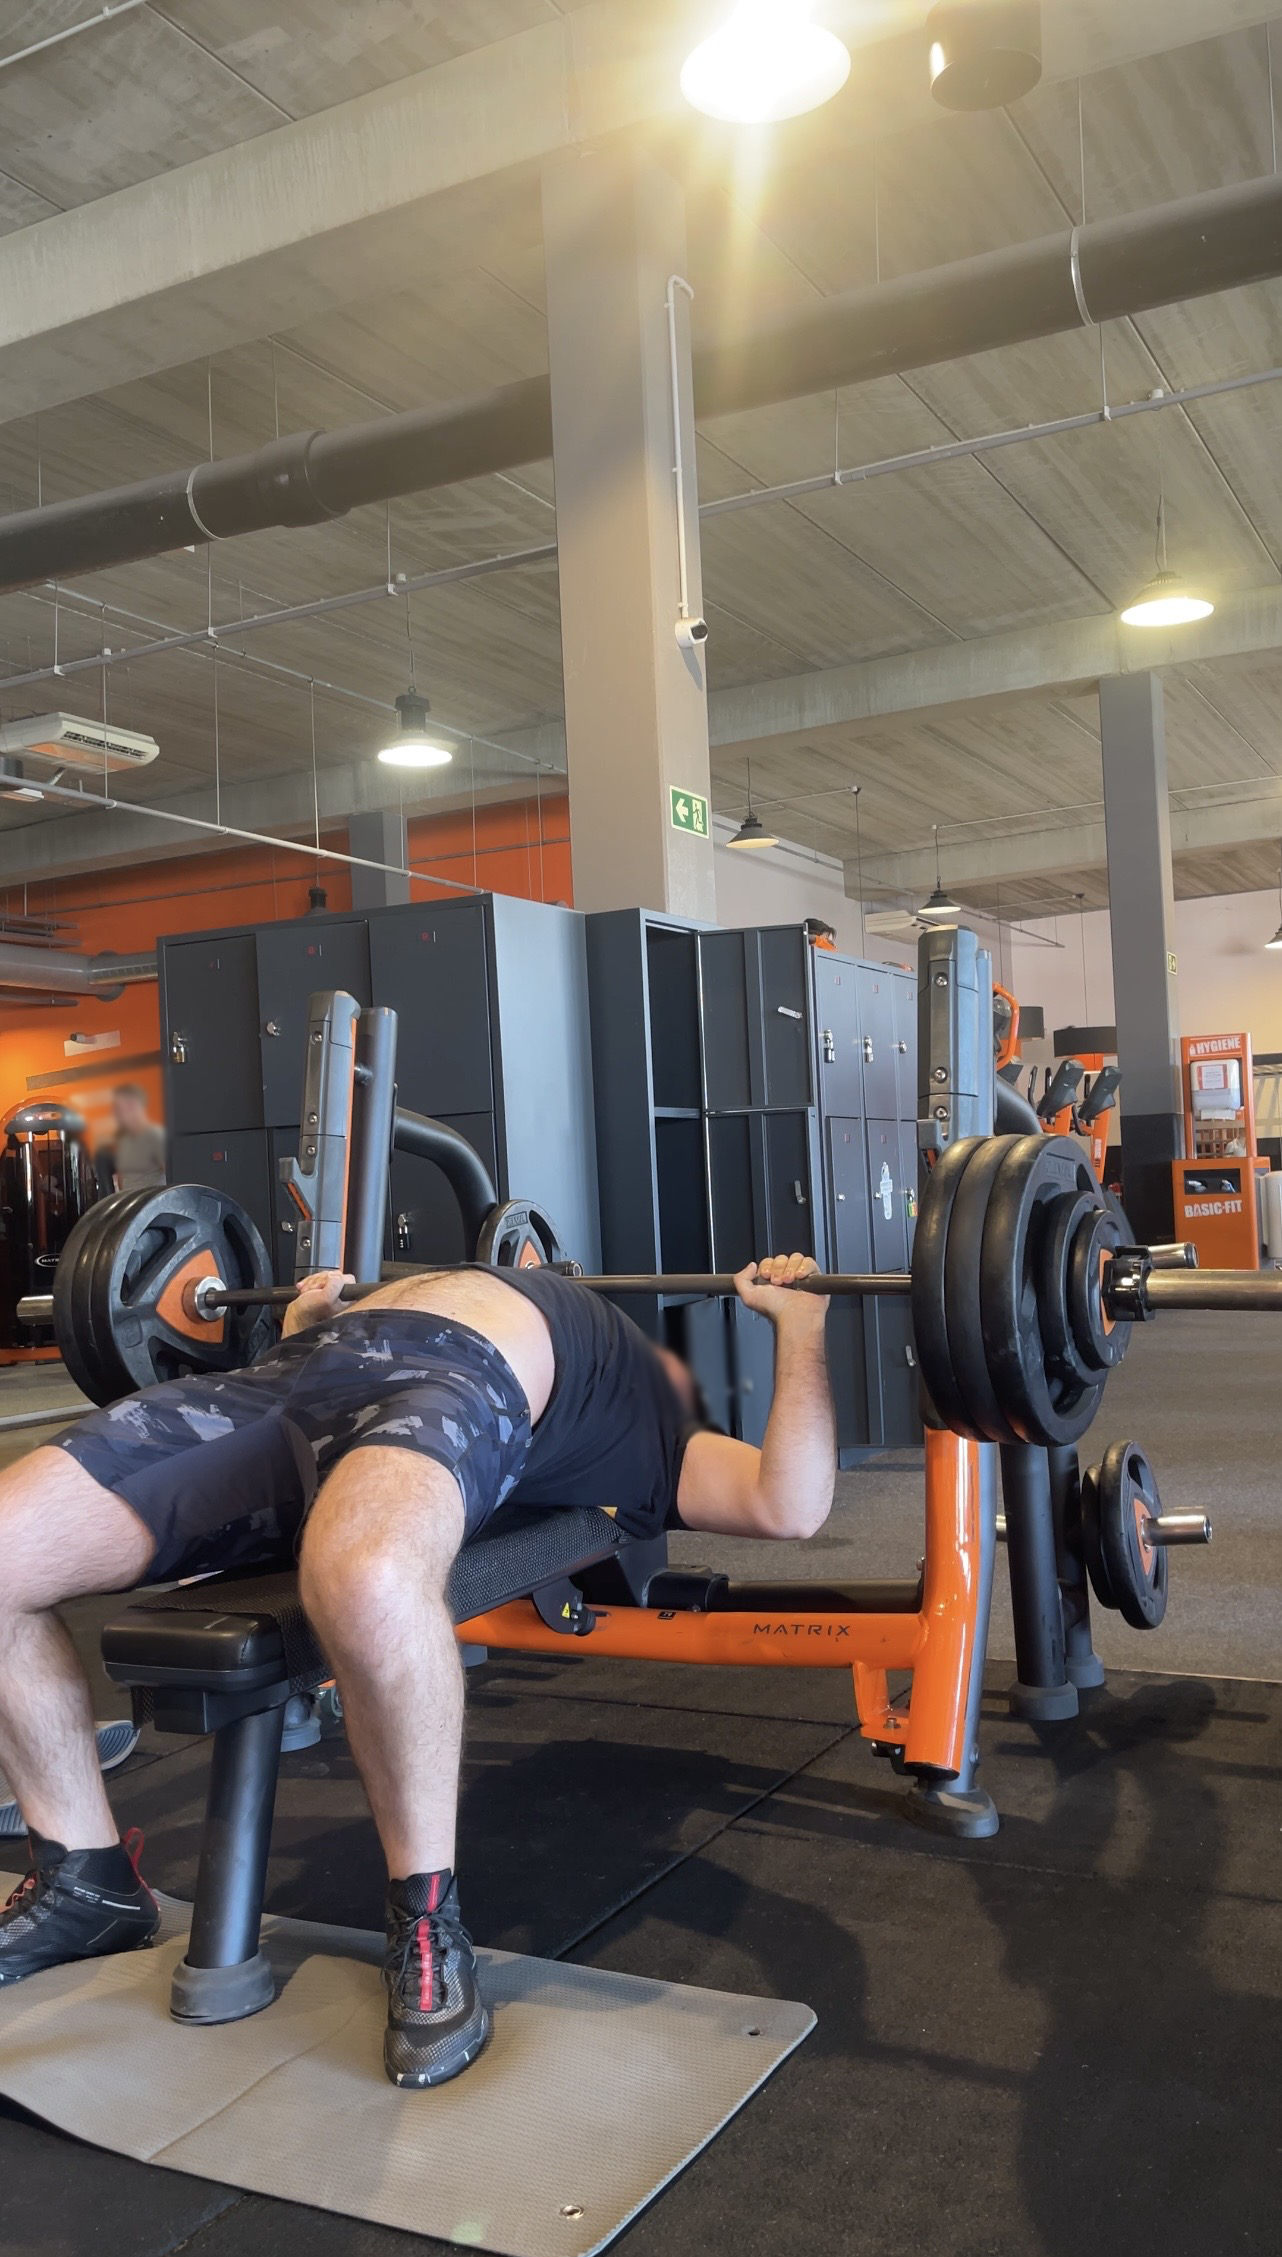
\includegraphics[width=3.5cm, height=5cm]{1-Introduction/2-Bench.jpg}
  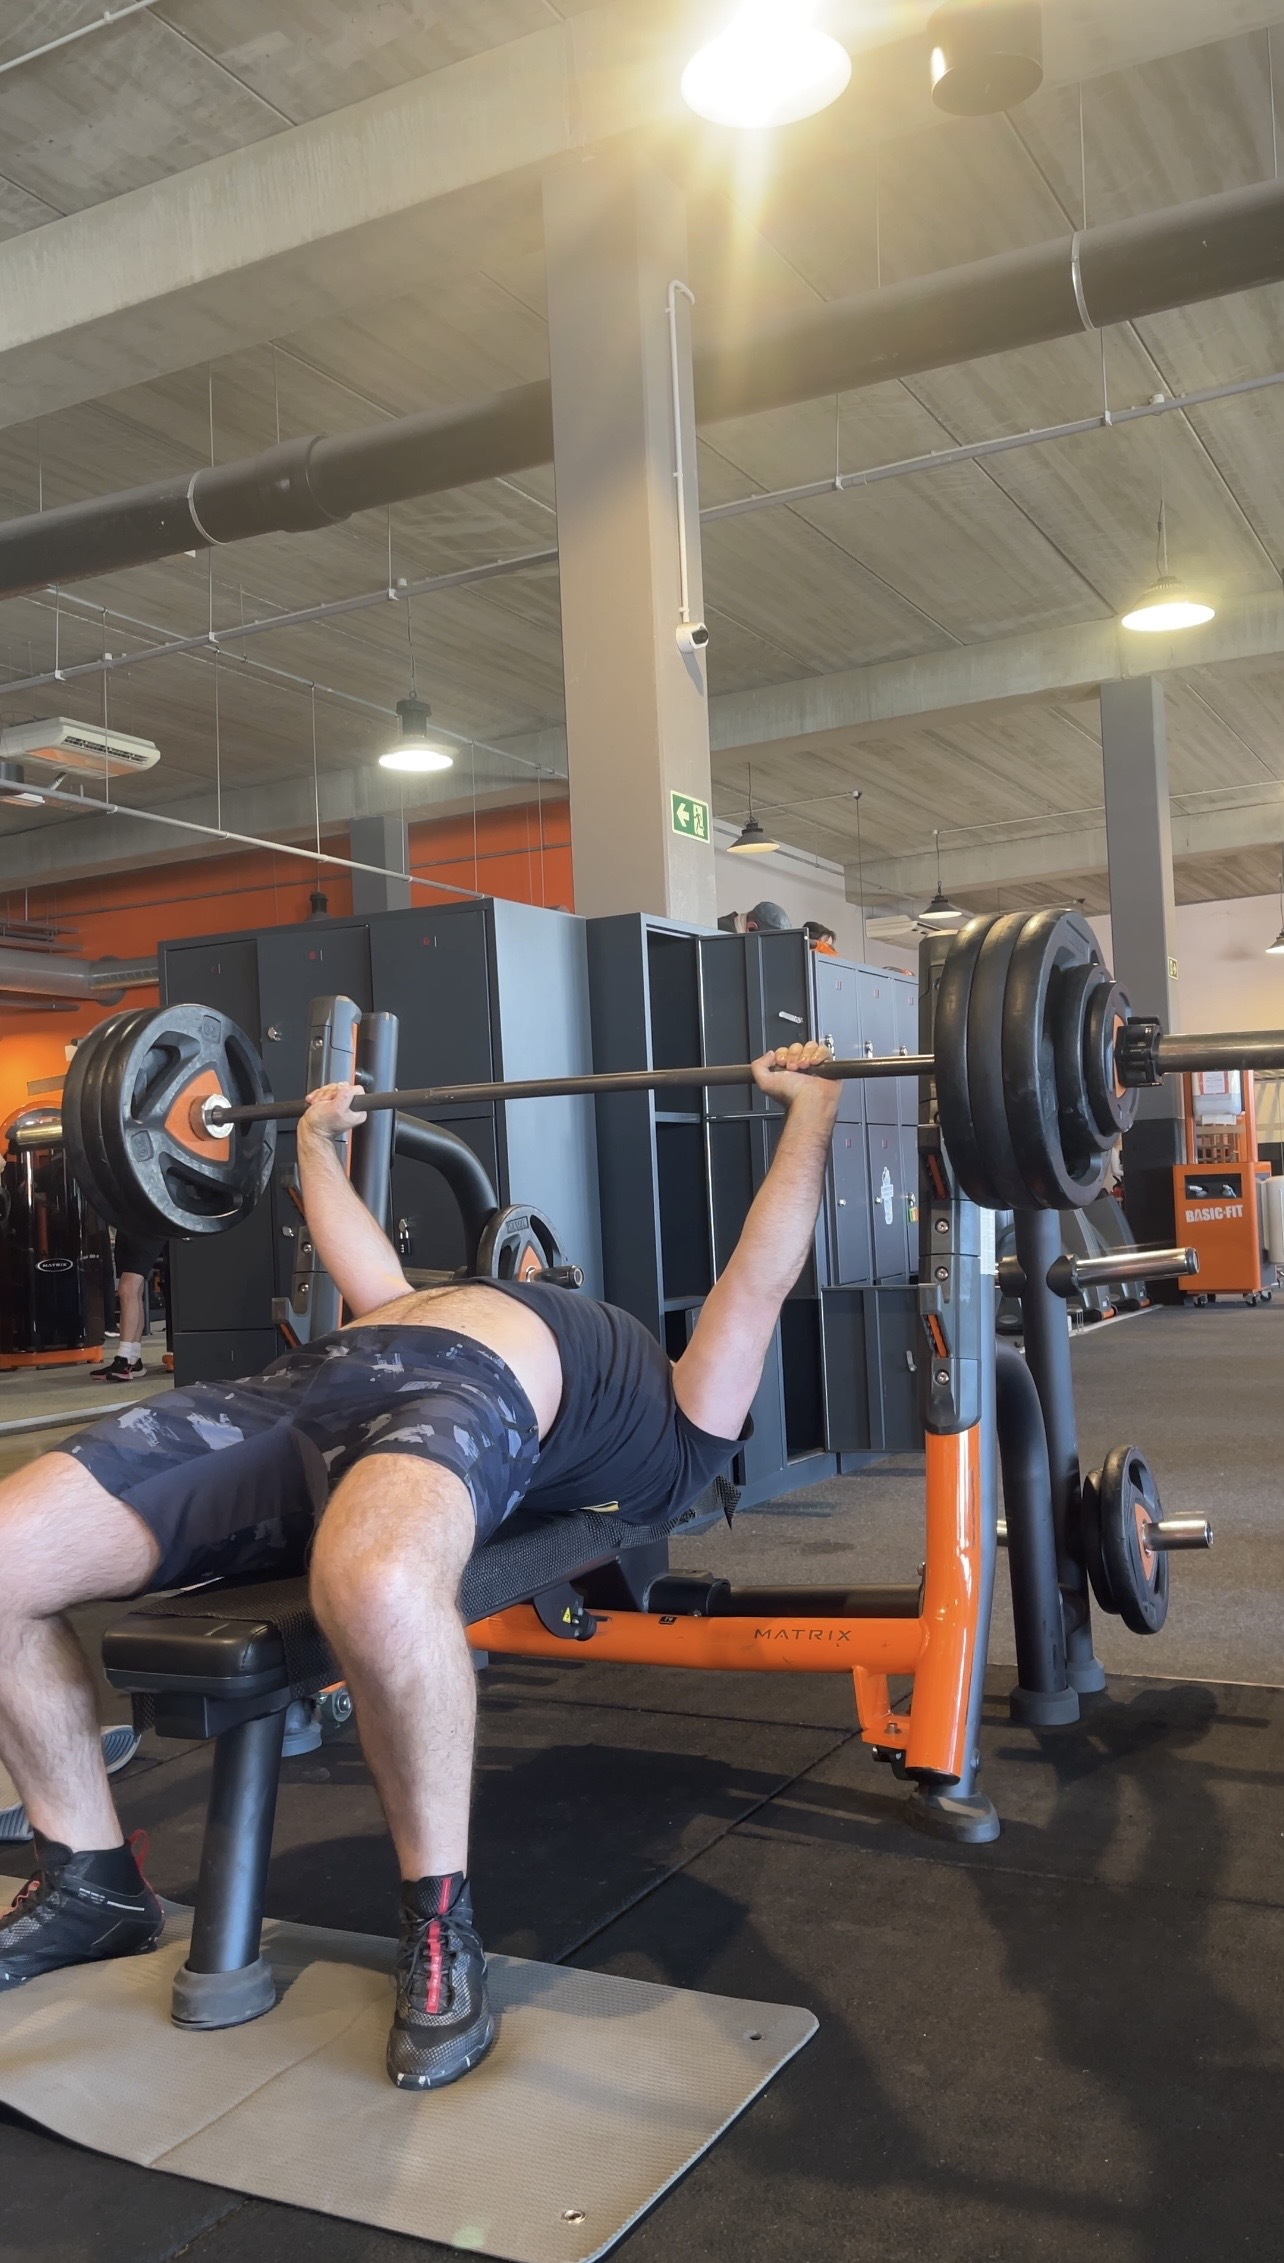
\includegraphics[width=3.5cm, height=5cm]{1-Introduction/3-Bench.jpg}
  \caption{Illustration d'un développé couché}
  \label{fig:bench}
\end{figure}

{\large \textbf{Soulevé de terre}}

Le soulevé de terre (figure~\ref{fig:deadlift}) consiste à soulever une barre chargée depuis le sol jusqu'à la position debout, genoux verrouillés et épaules en arrière. Le règlement technique de l'IPF en donne la définition suivante :

"Le force-athlétiste fera face à l'avant du plateau, la barre posée horizontalement devant ses pieds. Il la saisira des deux mains en utilisant la prise qu'il désirera (en pronation, en supination, ou inversée, mains à l'extérieur des cuisses, ou à l'intérieur), et la soulèvera jusqu'à ce qu'il se redresse complètement. À la fin du soulevé, le force-athlétiste doit être droit, genoux verrouillés, et les épaules en arrière. [...] toute redescente de la barre avant que le force-athlétiste atteigne sa position finale sera sanctionnée." \cite[p.~25]{IPF-Technical-Regulations-2025} 

\begin{figure}
  [htp]
  \centering
  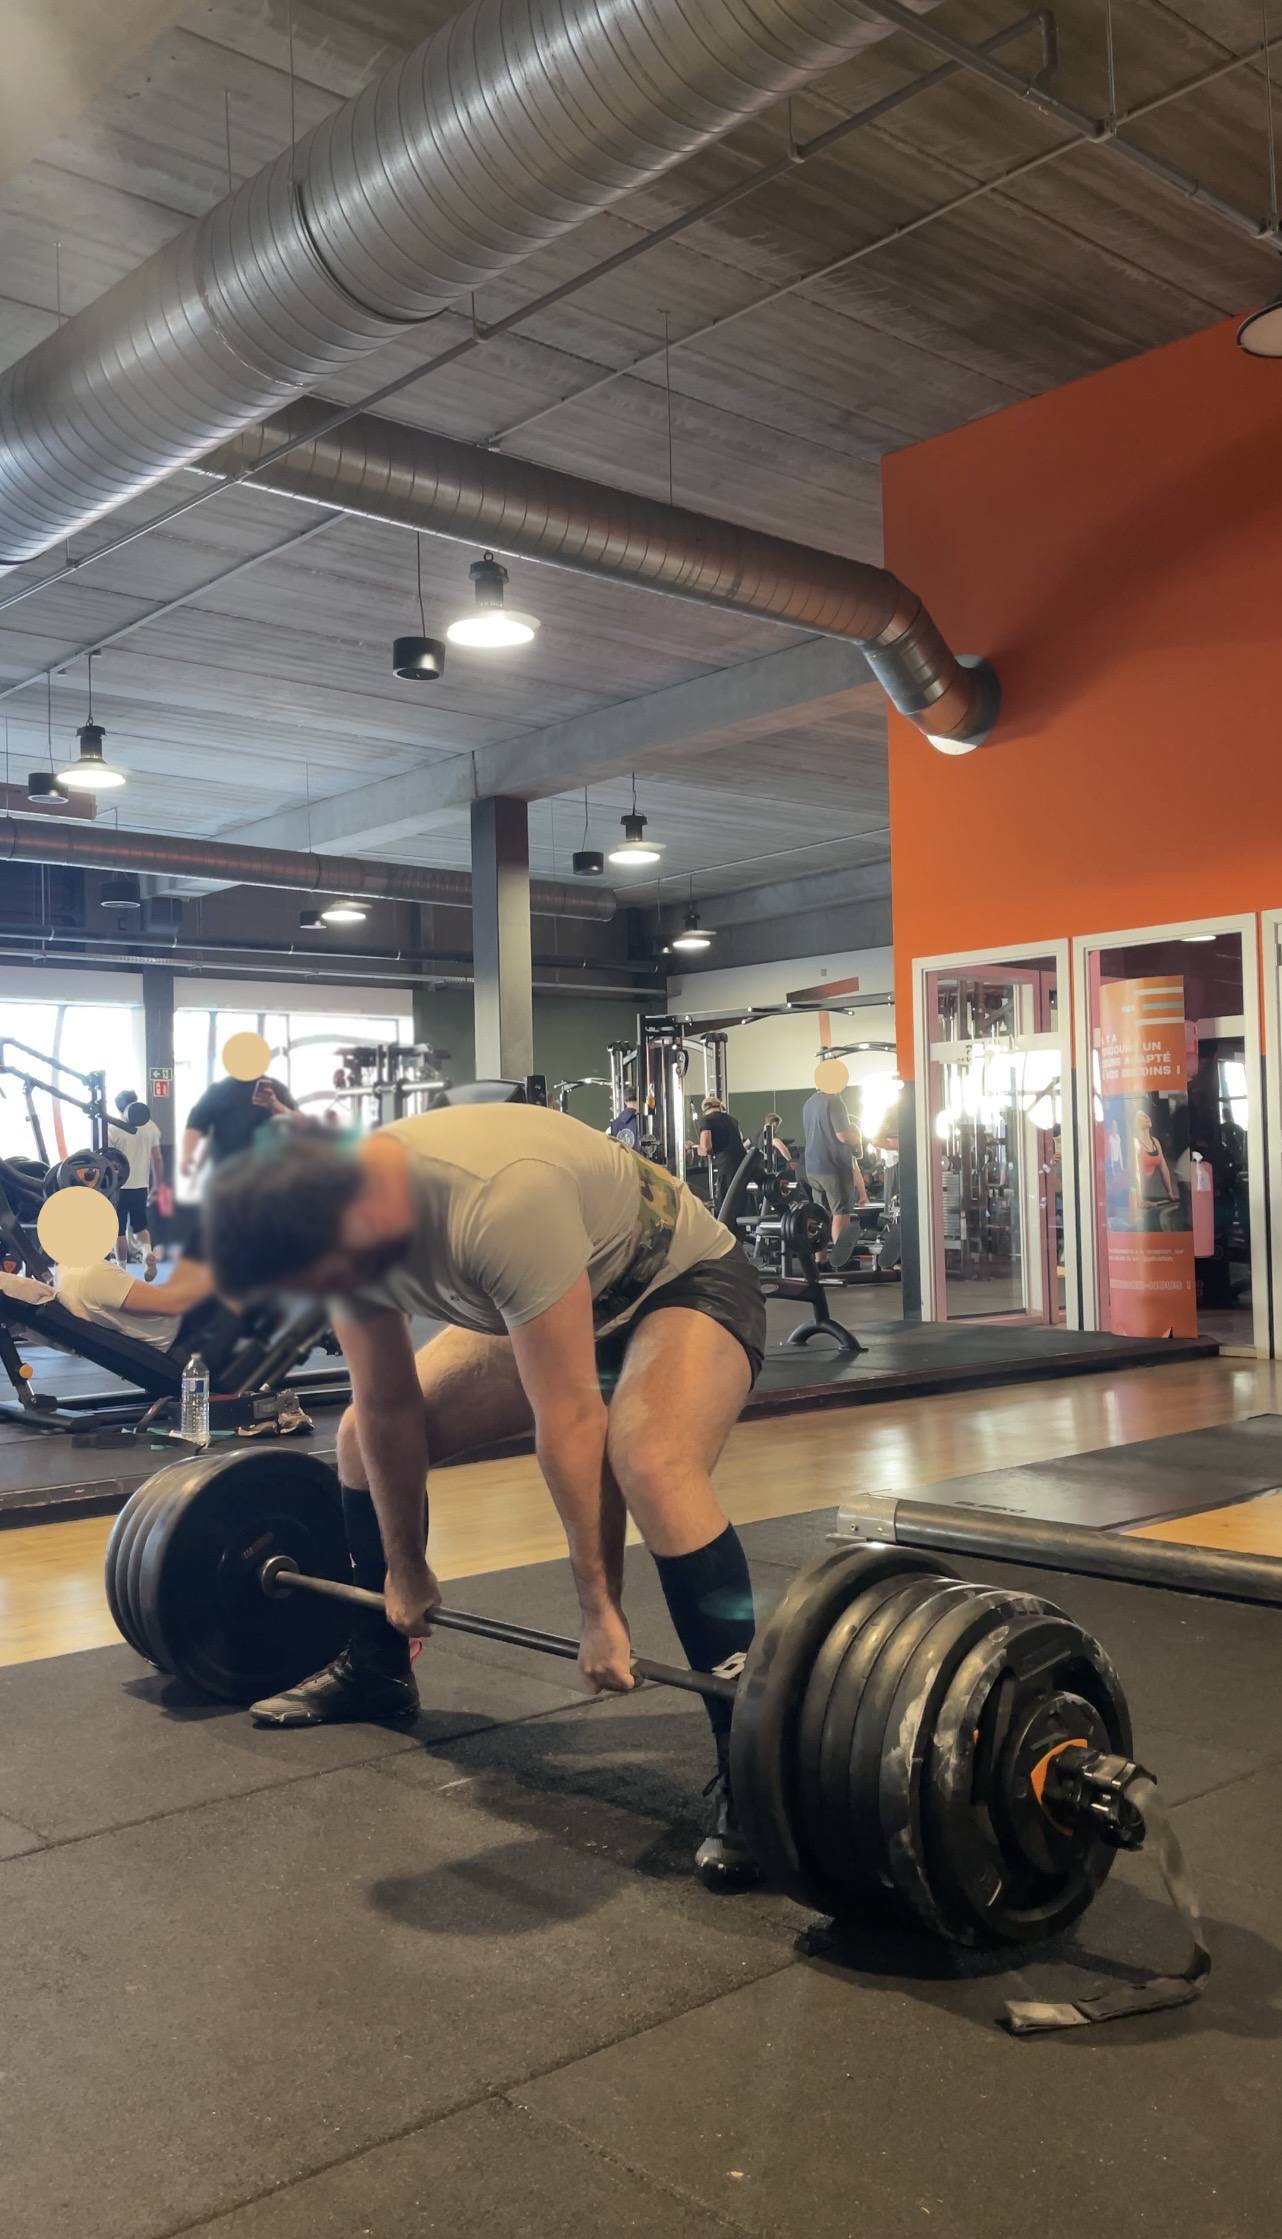
\includegraphics[width=3.5cm, height=5cm]{1-Introduction/1-Deadlift.jpg}
  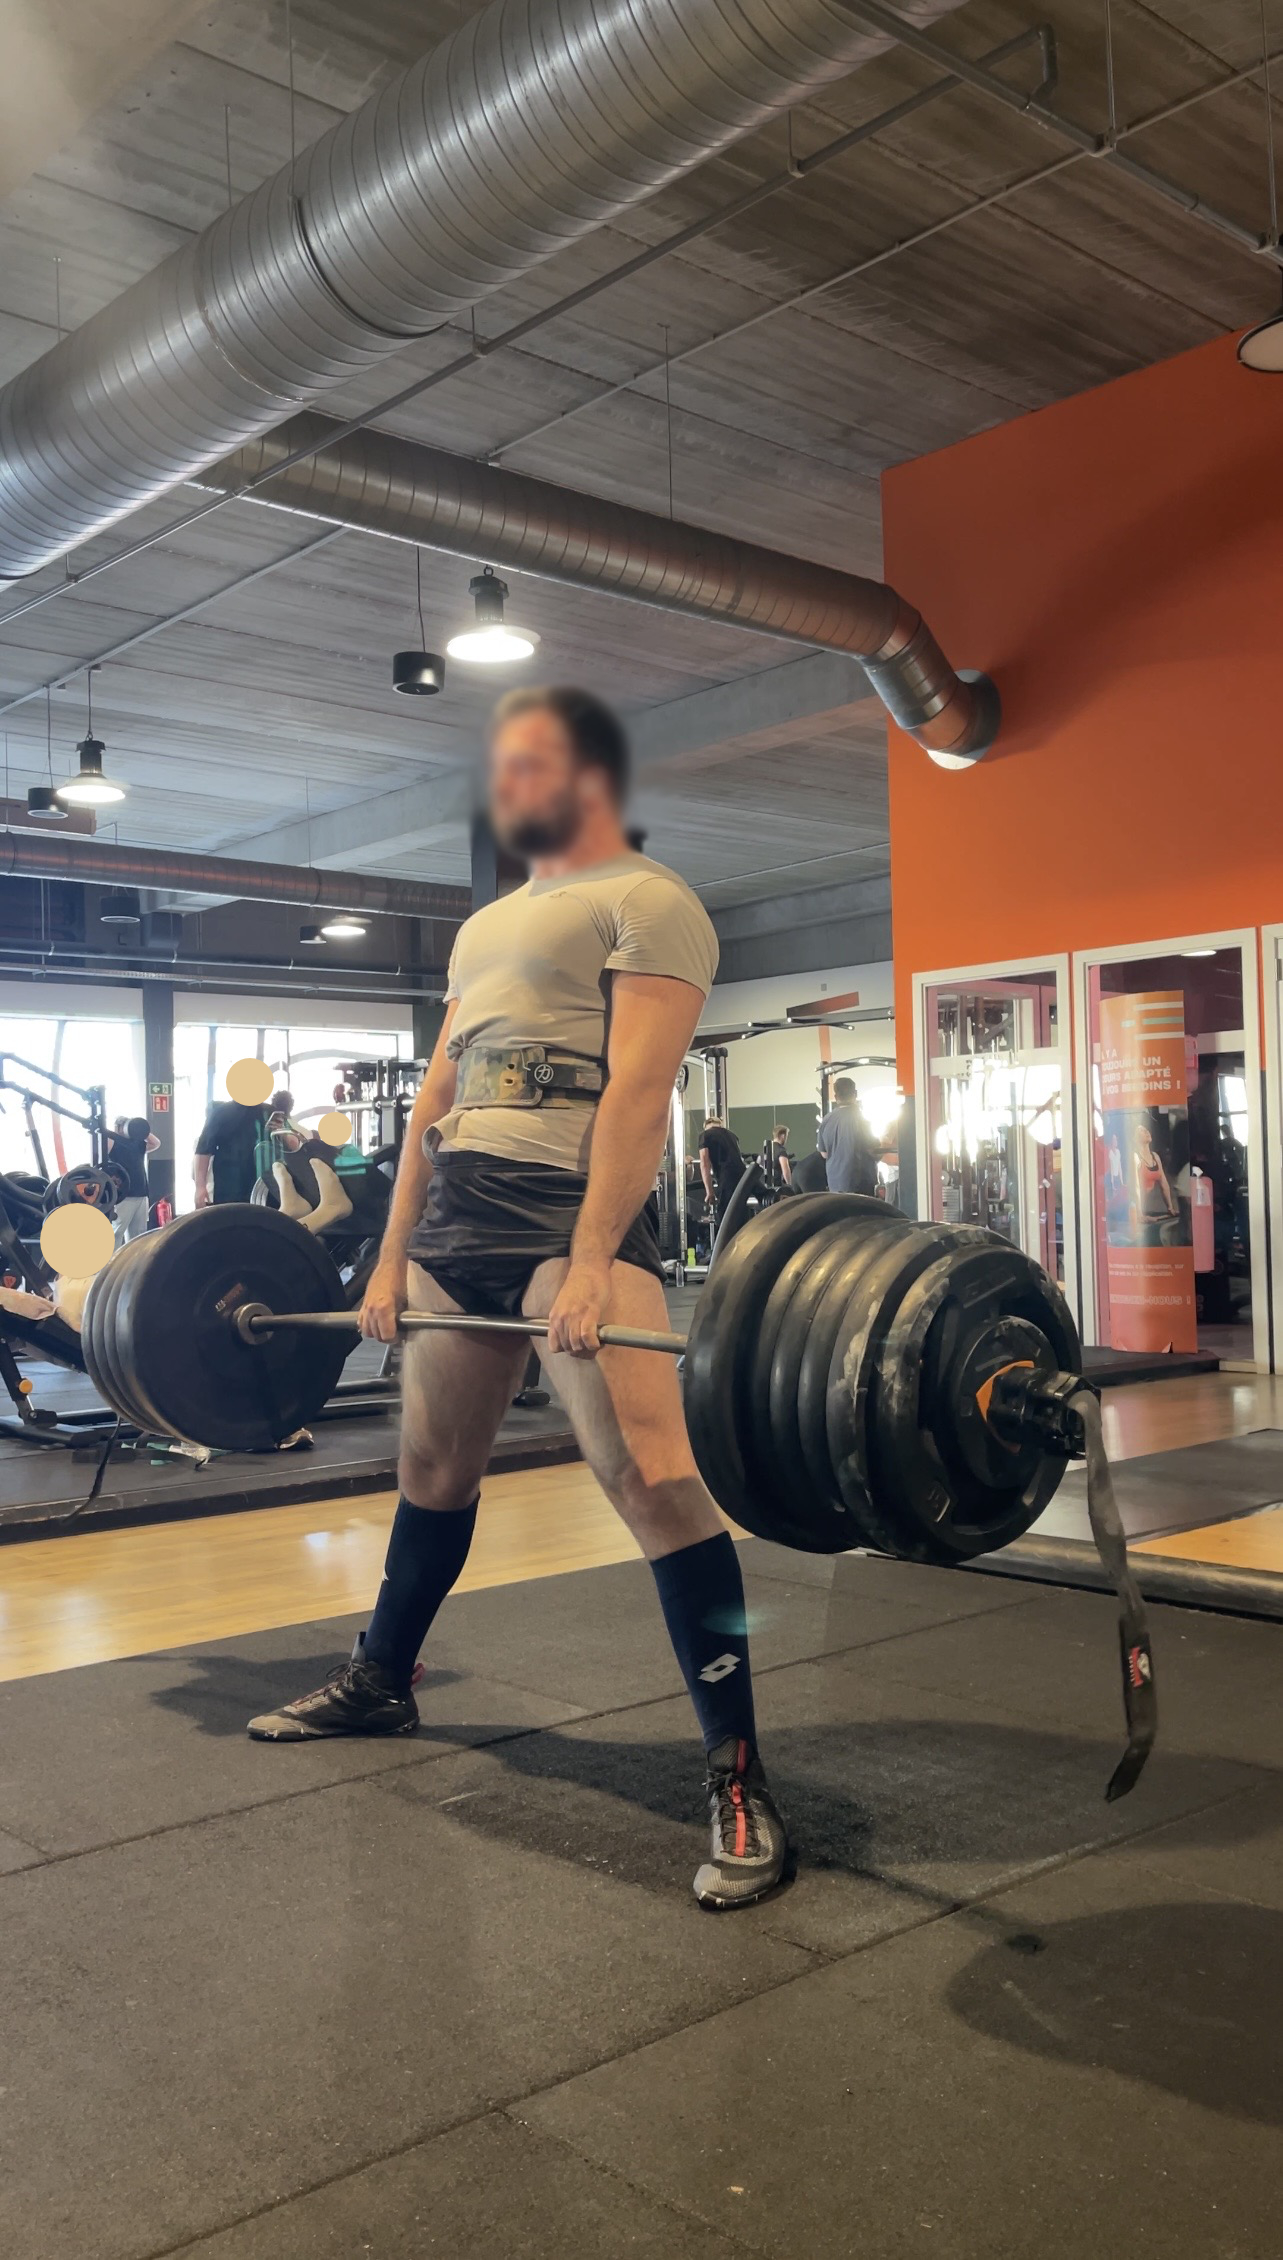
\includegraphics[width=3.5cm, height=5cm]{1-Introduction/2-Deadlift.jpg}
  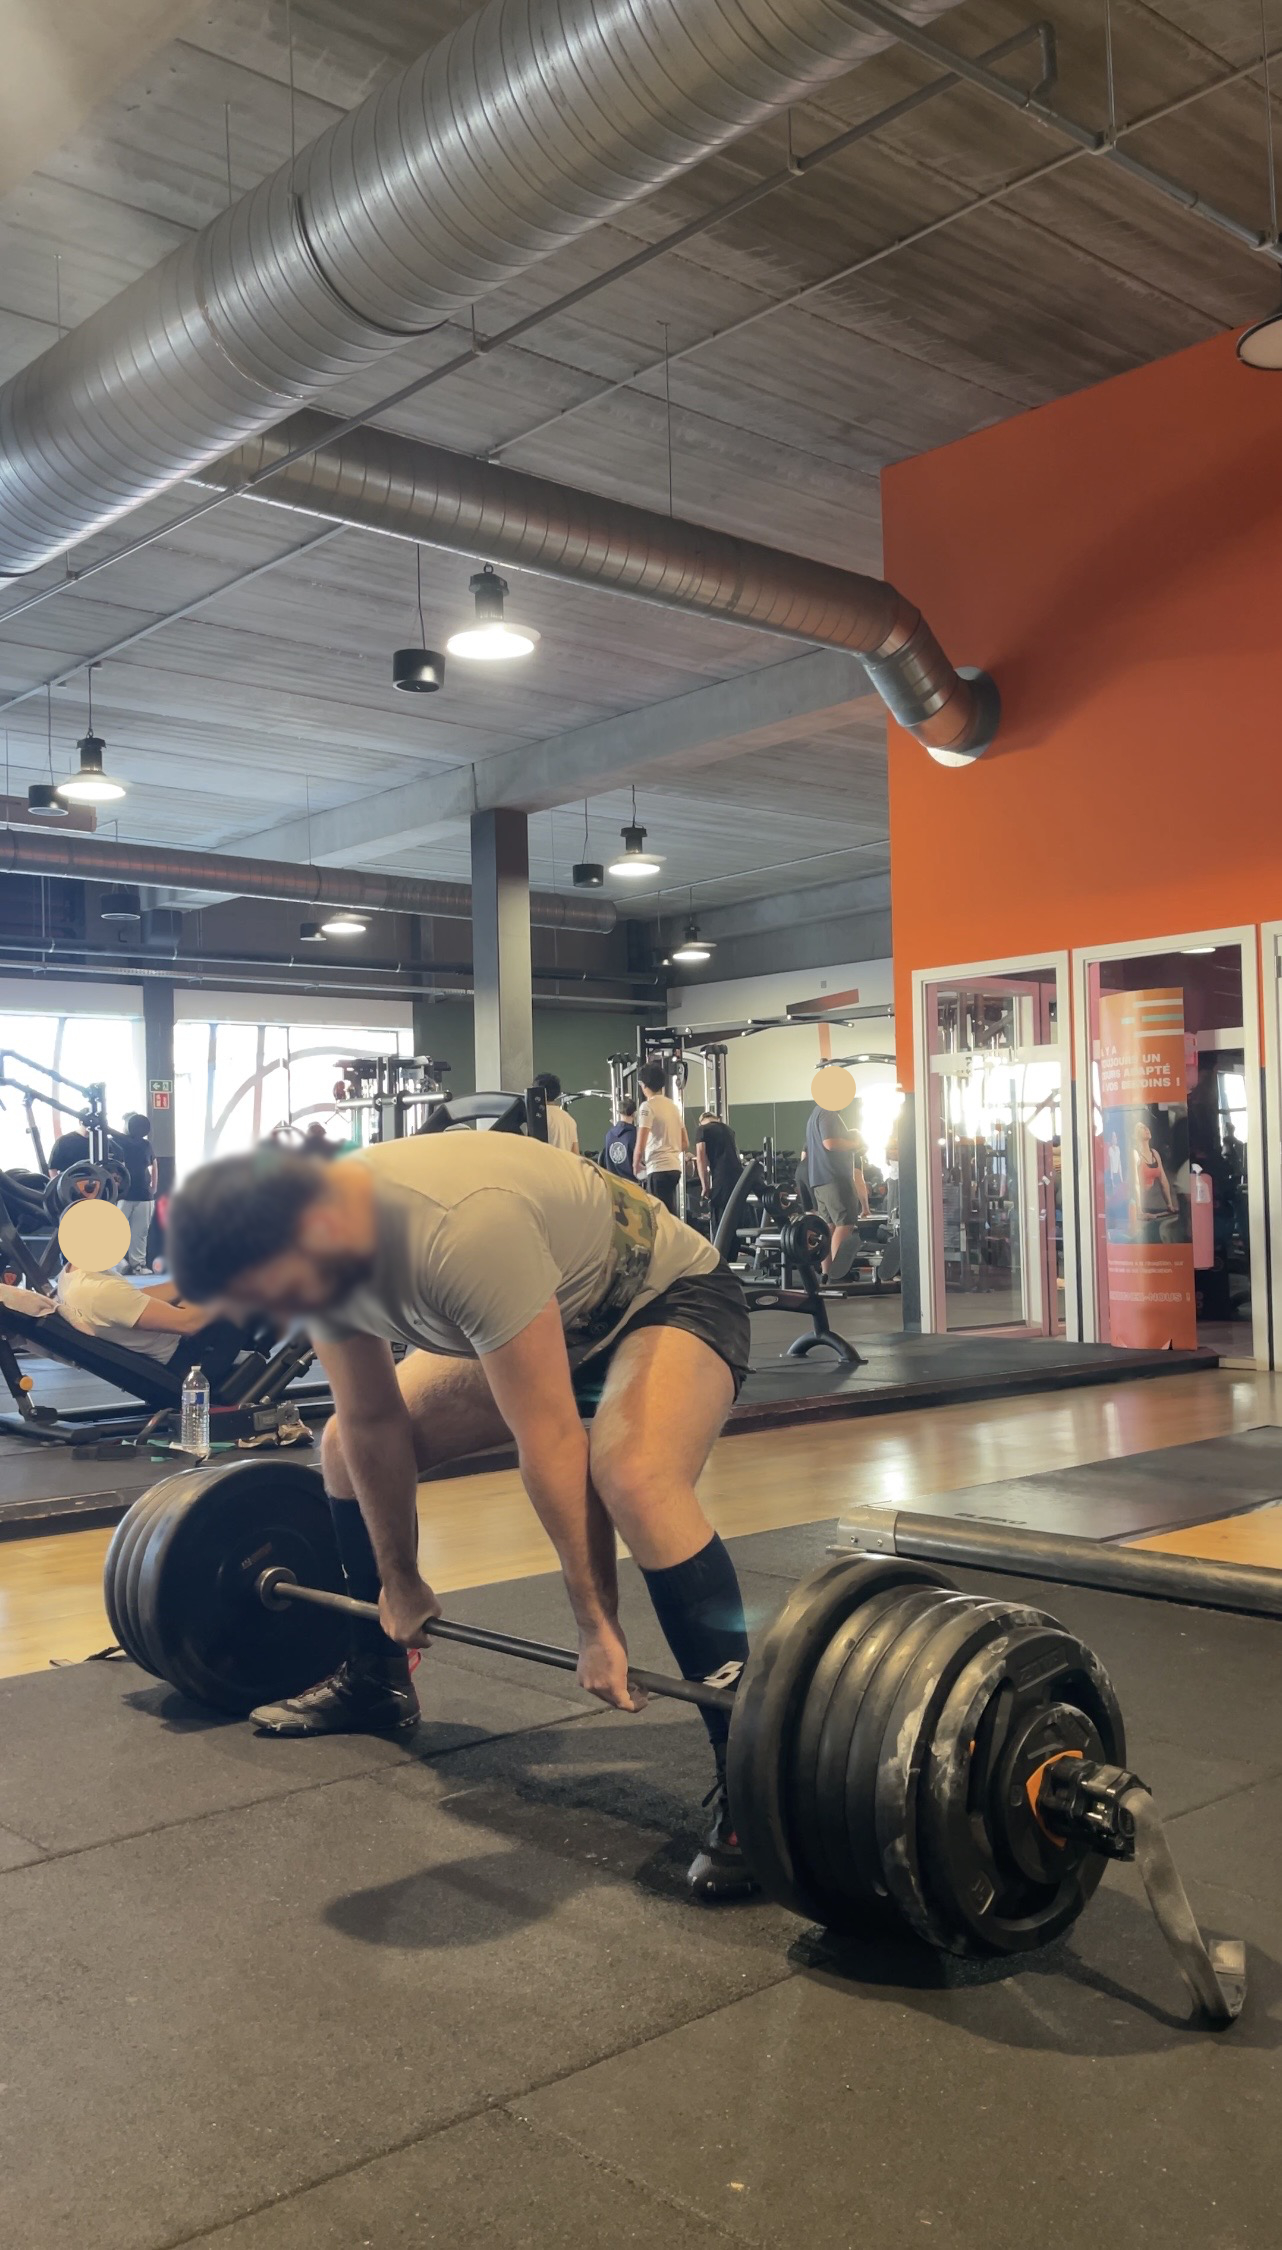
\includegraphics[width=3.5cm, height=5cm]{1-Introduction/3-Deadlift.jpg}
  \caption{Illustration d'un soulevé de terre}
  \label{fig:deadlift}
\end{figure}

{\large \textbf{Enjeux}}

La performance dans ce sport dépend de la capacité de l'athlète à déplacer une charge maximale tout en respectant des trajectoires motrices optimales. L'analyse biomécanique \footnote{La biomécanique est la discipline scientifique qui applique les principes de la 
mécanique (forces, moments, accélérations) à l'étude du mouvement du corps humain. En contexte sportif, elle permet de quantifier les contraintes articulaires, les leviers osseux et les trajectoires afin d'optimiser la technique et de prévenir les blessures.} joue donc un rôle fondamental pour trois raisons majeures :

\begin{itemize}
  \item \textbf{Optimisation de la performance} : L'étude des leviers articulaires et de la vitesse de barre permet d'identifier les points de rupture technique (\textit{sticking points}).

  \item \textbf{Prévention des blessures} : Une détection précoce des asymétries ou des inclinaisons pelviennes non conformes est essentielle pour limiter les contraintes sur le rachis \footnote{Le rachis (ou colonne vertébrale), est la structure osseuse centrale du squelette. Il constitue le principal axe de transmission des charges mécaniques lors des exercices de force athlétique, notamment au squat et au soulevé de terre.}.

  \item \textbf{Assistance à l'arbitrage} : En compétition, les juges évaluent la conformité de chaque mouvement aux critères techniques définis par le règlement de l'IPF\cite{IPF-Technical-Regulations-2025}, tels que la profondeur du squat ou le verrouillage des coudes au développé couché. Une reconstruction tridimensionnelle automatique offre une mesure objective et reproductible de ces critères, réduisant la part de subjectivité inhérente au jugement humain.
\end{itemize}

\section{Problématique : Limites des systèmes actuels} \label{one_two}

L'analyse du mouvement en force athlétique repose traditionnellement sur l'observation visuelle par un expert ou sur l'usage de caméras standards. Les failles de ces méthodes peuvent être mises en évidence afin de justifier l'apport d'une nouvelle technologie. Les difficultés rencontrées par les systèmes classiques se jouent autour de trois axes majeurs :

\begin{itemize}
  \item \textbf{Perte d'information spatiale} : Une capture vidéo standard projette un mouvement tridimensionnel (\textit{3D}) sur un plan bidimensionnel (\textit{2D}), entraînant des erreurs de parallaxe \footnote{La parallaxe désigne le déplacement apparent d'un objet observé depuis deux points de vue différents. En vision monoculaire, ce phénomène se manifeste lorsqu'un segment corporel incliné selon l'axe de profondeur est projeté sur le plan image avec des proportions apparentes différentes de ses proportions réelles, induisant des erreurs systématiques dans l'estimation des angles articulaires.}~\cite{Hartley2003} et une incapacité à mesurer les rotations transversales \footnote{Les rotations transversales désignent les rotations s'effectuant autour de l'axe vertical du corps (axe longitudinal), telles que la rotation du bassin ou du torse dans le plan horizontal. En force athlétique, une rotation transversale asymétrique du bassin lors d'un squat constitue un indicateur précoce de déséquilibre musculaire ou de limitation de mobilité.} ou les inclinaisons latérales du buste, pourtant critiques lors d'un squat ou d'un soulevé de terre.
  \item \textbf{Contraintes environnementales et occlusions} : Dans une salle de sport, la présence de disques, de racks à squat ou d'autres individus crée des occlusions partielles qui empêchent les algorithmes de détection de pose classiques de maintenir un suivi fluide et rigoureux~\cite{OpenPose-2019}.
  \item \textbf{Limites des capteurs inertiels\footnote{Un capteur inertiel (\emph{Inertial Measurement Unit}, IMU) est un dispositif électronique mesurant les forces d'accélération et les vitesses angulaires via un accéléromètre et un gyroscope, auxquels s'ajoute parfois un magnétomètre pour estimer l'orientation absolue.}} : Bien qu'ils fournissent des données numériques, les capteurs portables sont intrusifs, nécessitent une calibration complexe avant chaque essai et peuvent bouger durant le mouvement, faussant ainsi les mesures de trajectoire~\cite{Roetenberg2009, Camomilla2018} (voir annexe~\ref{ann:imu-tests}).
\end{itemize}

Il est donc fondamental de proposer une méthode capable de reconstruire précisément la géométrie du corps en trois dimensions sans marqueurs physiques, afin de transformer une simple vidéo en un outil d'analyse précis. Une telle approche, ne nécessitant aucun équipement spécialisé au-delà d'une caméra standard, rend l'analyse biomécanique accessible aux athlètes amateurs et aux entraîneurs ne disposant pas d'un laboratoire de biomécanique.

\section{Objectifs et contributions du travail} \label{one_three}

L'objectif central de ce mémoire est de concevoir une méthode et des principes pour améliorer l'analyse technique en force athlétique grâce à l'intelligence artificielle (\textit{IA}). Pour répondre aux problématiques identifiées, une architecture logicielle reposant sur quatre piliers technologiques est proposée : la segmentation sémantique, l'estimation de profondeur monoculaire, la complétion amodale des occlusions et la reconstruction tridimensionnelle de la pose.

L'apport personnel de ce travail réside dans l'individualisation du modèle de complétion amodale des occlusions ainsi qu'à l'unification de ces outils au sein d'un pipeline complet, permettant de passer d'une ressource vidéo brute à une représentation posturale en trois dimensions.

\section{Organisation du mémoire} \label{one_four}

Ce document structure la progression méthodologique et expérimentale de l'architecture développée. Il s'articule autour des chapitres suivants :

\textbf{Chapitre 2 - État de l'art :} Synthétise les limites des méthodes de l'analyse biomécanique traditionnelles et les apports de l'intelligence artificielle, puis présente les modèles fondamentaux utilisés dans le pipeline : segmentation vidéo, estimation de profondeur monoculaire, complétion amodale des occlusions et estimation de pose 3D.

\textbf{Chapitre 3 - Architecture du pipeline :} Détaille l'intégration des réseaux de neurones artificiels (SAM3, MoGe, TACO et SAM-3D Body) et justifie les choix techniques assurant la synchronisation du flux de données.

\textbf{Chapitre 4 - Dataset et fine-tuning du modèle de diffusion :} Décrit la méthodologie de constitution du jeu de données, la stratégie d'annotation des occlusions, ainsi que les protocoles d'entraînement et d'évaluation du modèle de complétion amodale.

\textbf{Chapitre 5 - Expérimentations et résultats :} Quantifie les performances du fine-tuning sur les trois mouvements de force athlétique via les métriques SSIM et LPIPS, évalue son impact sur la reconstruction 3D produite par SAM 3D Body via le MPJPE, et analyse le cas limite identifié sur le jeu de données de tests.

\textbf{Chapitre 6 - Conclusion et perspectives :} Dresse le bilan objectif des contributions, décrit les limites matérielles et algorithmiques persistantes, et oriente les futurs axes de développement.
% ---------------------
% ETAT DE L'ART
% ---------------------
\chapter{État de l'art} \label{ch_two}

L'analyse de la posture humaine par vision par ordinateur a connu un tournant avec la montée en popularité des réseaux de neurones profonds~\cite{Human-Pose-Estimation-2021}. Ce chapitre recense les avancées théoriques et les modèles architecturaux nécessaires à la compréhension du pipeline proposé pour la de reconstruction 3D, en partant des méthodes traditionnelles de l'analyse biomécanique en force athlétique jusqu'aux architectures d'apprentissage profond les plus récentes.

\section{Analyse biomécanique en force athlétique} 

L'analyse biomécanique en force athlétique s'effectue majoritairement par trois approches complémentaires. La première repose sur la vidéo standard, analysée manuellement pour évaluer la trajectoire de la barre ainsi que le mouvement de l'individu. Cette analyse peut être biaisée par l'angle de vue, ainsi que les conditions de capture (occlusions, éclairage, qualité vidéo). La deuxième utilise des transducteurs linéaires de position\footnote{Un transducteur linéaire de position (également appelé \emph{encoder} ou \emph{linear position transducer}) est un capteur mécanique-électrique composé d'un boîtier fixé à une structure rigide et d'un câble rétractable attaché à la barre. Le déplacement de la barre déroule le câble, dont la longueur est convertie en signal électrique via un potentiomètre ou un encodeur rotatif. La dérivée temporelle de ce signal fournit la vitesse instantanée de la barre, et sa dérivée seconde l'accélération, avec une précision typique inférieure au millimètre.} qui permettent de convertir un déplacement mécanique, via une corde fixée à la barre, en un signal électrique mesurable, permettant de calculer sa vitesse et son accélération avec une grande précision~\cite{MorenoVillanueva2021}. Ces appareils sont encombrants et relativement chers car ils sont la plupart du temps liés à une application mobile propriétaire. La troisième fait appel à des centrales inertielles (\textit{IMU}) placées sur la barre, fournissant des données d'orientation en temps réel mais au prix d'une calibration complexe~\cite{Abbott2020, Camomilla2018}.

Au-delà de ces approches instrumentales, la capture de mouvement (\textit{motion capture} ou \textit{mocap}) offre une représentation plus complète du mouvement dans l'espace tridimensionnel.

La capture de mouvement désigne l'ensemble des techniques permettant d'enregistrer le mouvement d'un corps dans l'espace et de le représenter sous forme de données numériques exploitables. On distingue deux grandes familles.

\textbf{Les systèmes à marqueurs} (\textit{marker-based mocap}) constituent la référence en laboratoire~\cite{Colwell2025}. Ils s'appuient sur des capteurs placés sur les segments corporels, dont la position est triangulée par un réseau de caméras. Ces systèmes offrent une précision sous le millimétrique mais sont intrusifs, coûteux, et imposent un environnement contrôlé incompatible avec une salle de sport~\cite{Tibrewal2024}.

\textbf{Les systèmes sans marqueurs} (\textit{markerless mocap}) estiment la pose  corporelle directement depuis les images, sans équipement sur le sujet. Portés par les avancées de l'apprentissage profond, ces systèmes connaissent un essor important. Des solutions comme OpenCap~\cite{Opencap-2026} ou Theia3D~\cite{Theia-3D-2026} permettent aujourd'hui d'obtenir des estimations cinématiques proches de la qualité avec marqueurs dans des conditions semi-contrôlées, à partir de plusieurs caméras synchronisées. Dans un contexte monoculaire, la tâche est plus difficile~\cite{Wade2022} : la perte d'information sur l'axe de profondeur introduit des ambiguïtés que les modèles paramétriques du corps humain (SMPL~\cite{SMPL-2015}, MHR~\cite{MHR-2025}) cherchent à lever en s'appuyant sur des données morphologiques apprises.

L'application de la capture de mouvement tridimensionnelle sans marqueurs à la force athlétique reste cependant sous-exploitée. Plusieurs facteurs l'expliquent : l'environnement complexe des salles de compétition (éclairage, encombrement, présence de plusieurs personnes), les occlusions fréquentes générées par la barre et les disques. Les travaux appliquant la \textit{mocap markerless} se limitent à des environnements contrôlés avec plusieurs caméras synchronisées, rendant leur déploiement en conditions réelles difficile. C'est précisément ce problème qu'un pipeline opérant depuis une unique caméra monoculaire non calibrée, telle que celle développée dans ce mémoire, cherche à résoudre.

\section{Limites des approches traditionnelles}

Les méthodes d'analyse biomécanique présentées à la section précédente partagent des limitations structurelles qui restreignent leur déploiement en conditions réelles d'entraînement et de compétition.

\subsection{Biais et subjectivité de l'analyse vidéo manuelle}

L'analyse vidéo manuelle reste la méthode la plus répandue chez les entraîneurs~\cite{Colyer-2018}, mais elle souffre de plusieurs biais inhérents. La qualité de l'évaluation dépend directement de l'expertise de l'observateur et de l'angle de capture choisi. Une vue de face ne permet pas d'évaluer l'inclinaison du buste, une vue de côté masque les asymétries latérales. Par ailleurs, les occlusions générées par la barre et les disques obstruent précisément les régions articulaires les plus importantes (épaules, hanches et genoux), rendant toute évaluation visuelle partielle et potentiellement erronée.

\subsection{Intrusivité des capteurs physiques}

Les transducteurs linéaires de position et les centrales inertielles fournissent des données précises sur la vitesse de la barre, mais ne donne aucune information sur la posture corporelle de l'athlète. De plus, leur installation est chronophage et nécessite souvent une calibration, ce qui les rend peu pratiques pour une utilisation régulière en salle de sport ou en compétition. Leur coût élevé et leur nature intrusive limitent également leur adoption à grande échelle, en particulier dans les contextes amateurs ou semi-professionnels.

\subsection{Contraintes des systèmes de capture de mouvement}

Les systèmes \textit{marker-based} offrent la meilleure précision disponible, mais leur déploiement exige un environnement expérimental contrôlé : placement minutieux des marqueurs sur le sujet, calibration du réseau de caméras, absence d'occlusions entre marqueurs et caméras. Ces conditions sont incompatibles avec une salle de sport standard, où l'encombrement, l'éclairage variable et la présence de plusieurs personnes invalident les hypothèses de fonctionnement du système.

Les systèmes \textit{markerless} lèvent la contrainte des marqueurs physiques mais requièrent à leur tour plusieurs caméras synchronisées et calibrées pour lever l'ambiguïté de profondeur. Des solutions comme OpenCap~\cite{Opencap-2026} ou Theia3D~\cite{Theia-3D-2026} restent ainsi dépendantes d'une infrastructure multi-caméras fixe, peu compatible avec les contraintes logistiques d'une compétition ou d'une salle d'entraînement commerciale.

\subsection{Occlusions non gérées}

Aucune des approches traditionnelles ne dispose de mécanisme pour gérer les occlusions générées par l'équipement de force athlétique. Or, lors d'un squat chargé, la barre et les disques masquent en permanence une portion significative du torse et des épaules de l'individu. Lors d'un développé couché, ils masquent une grande partie du tronc ainsi que les bras et les épaules. Ces occlusions constituent un cas d'échec systématique pour les algorithmes d'estimation de pose classiques, qui produisent des points articulaires (\textit{keypoints}) \footnote{Les \textit{keypoints} désignent les points caractéristiques du corps humain utilisés pour représenter la pose squelettique : articulations principales (épaules, coudes, poignets, hanches, genoux, chevilles) et extrémités (tête, mains, pieds). Leur localisation précise dans l'image constitue la sortie principale des modèles d'estimation de pose.} absents ou mal localisés (figure~\ref{fig:occlusion-example}) dès qu'une partie du corps disparaît du champ visuel, sans mécanisme de reconstruction des parties manquantes.

\begin{figure}
  [htp]
  \centering
  \includegraphics[width=12cm, height=5cm]{2-State_of_the_art/Example-occlusion.jpg}
  \caption{Illustration d'une occlusion non gérée}
  \label{fig:occlusion-example}
\end{figure}

\medskip

L'ensemble de ces limitations justifie le recours à une approche fondée sur l'apprentissage profond et la vision par ordinateur, capable d'opérer depuis une unique caméra monoculaire non calibrée tout en gérant explicitement les occlusions propres à la force athlétique.


\section{Apports de l'intelligence artificielle et de la vision par ordinateur}

Face aux limitations identifiées à la section précédente, l'intelligence artificielle et la vision par ordinateur offrent de nouvelles perspectives dans les possibilités d'analyse biomécanique. Cette section présente et détaille ces perspectives.

\subsection{Passage de la mesure instrumentale à l'inférence visuelle}

L'apprentissage profond permet de substituer les capteurs physiques par des modèles capables d'inférer directement depuis le flux vidéo. Cette substitution élimine les contraintes d'intrusivité et de calibration associées aux IMU et aux transducteurs, tout en rendant l'analyse accessible depuis un équipement aussi courant qu'un smartphone ou une caméra.

\subsection{Robustesse aux occlusions par les modèles génératifs}

Les modèles de diffusion introduisent la capacité de reconstruire les régions corporelles masquées par l'équipement, là où les approches traditionnelles produisent des données manquantes ou erronées. Cette complétion amodale, rendue possible par la connaissance implicite de l'anatomie humaine acquise lors du pré-entraînement, permet de fournir aux modules d'estimation de pose une topologie corporelle complète, même en présence d'occlusions massives.

\subsection{Reconstruction tridimensionnelle monoculaire}

Les modèles paramétriques du corps humain (SMPL~\cite{SMPL-2015}, MHR~\cite{MHR-2025}), combinés aux architectures d'estimation de profondeur monoculaire, permettent de lever l'ambiguïté de profondeur sans recourir à plusieurs caméras synchronisées. La reconstruction 3D devient ainsi réalisable depuis une unique caméra non calibrée, dans des conditions d'éclairage et d'encombrement non contrôlées, ce qui constitue précisément le contexte des salles d'entraînement et des compétitions de force athlétique.

\subsection{Généralisation sans annotation spécifique}

Les architectures fondationnelles entraînées à très grande échelle (SAM~\cite{SAM-2023}, SAM 2~\cite{SAM2-2024}, SAM 3~\cite{SAM3-2025}) présentent des capacités de généralisation \textit{zero-shot} \footnote{L'inférence \textit{zero-shot} désigne la capacité d'un modèle à traiter des catégories ou des domaines non rencontrés lors de son entraînement, sans exemples supplémentaires ni réentraînement. Cette propriété, rendue possible par l'entraînement à très grande échelle sur des données hétérogènes, est déterminante dans des contextes applicatifs où les données annotées spécifiques au domaine sont rares ou inexistantes, comme c'est le cas pour la force athlétique.}. : elles produisent des résultats exploitables sur des domaines non vus lors de l'entraînement, sans nécessiter d'annotations spécifiques à la force athlétique. Cette propriété est déterminante dans un contexte où les données annotées de force athlétique sont quasi inexistantes dans les corpus publics.

\section{Segmentation d'instances vidéo} 

La segmentation d'instances vidéo (\textit{Video Instance Segmentation}, VIS) exige la détection, la délimitation spatiale et le suivi temporel d'entités spécifiques. Historiquement dominée par des modèles basés sur les réseaux de neurones convolutifs (\textit{Convolutional Neural Network}, CNN) (par exemple : Mask R-CNN~\cite{Mask-R-CNN-2018}), la discipline a muté vers les architectures fondationnelles. L'introduction du \textit{Segment Anything Model} (\textit{SAM})~\cite{SAM-2023} et de ses itérations intégrant la dimension temporelle (\textit{SAM 2}~\cite{SAM2-2024}, \textit{SAM 3}~\cite{SAM3-2025}) permet la génération de masques de haute fidélité zero-shot. Ces réseaux exploitent des transformeurs de vision \footnote{Les transformeurs de vision (\emph{Vision Transformers}, ViT) sont des architectures d'apprentissage profond qui appliquent le mécanisme d'attention (\emph{self-attention}) au traitement des images en découpant celles-ci en patches traités comme des séquences de tokens. Contrairement aux CNN, ils capturent des dépendances globales entre régions distantes de l'image dès les premières couches, ce qui les rend particulièrement robustes aux occlusions partielles.} et des mécanismes de mémoire spatio-temporelle \footnote{Un mécanisme de mémoire spatio-temporelle désigne une composante architecturale permettant au modèle de conserver et d'utiliser des représentations issues de trames précédentes lors du traitement d'une nouvelle trame.} pour maintenir l'identité de l'objet malgré les déformations dynamiques rapides. Dans l'analyse sportive, la segmentation garantit l'isolation de la géométrie de l'athlète des objets en premier ou en arrière-plan (figure~\ref{fig:segment-illustration}).

\begin{figure}
  [htp]
  \centering
  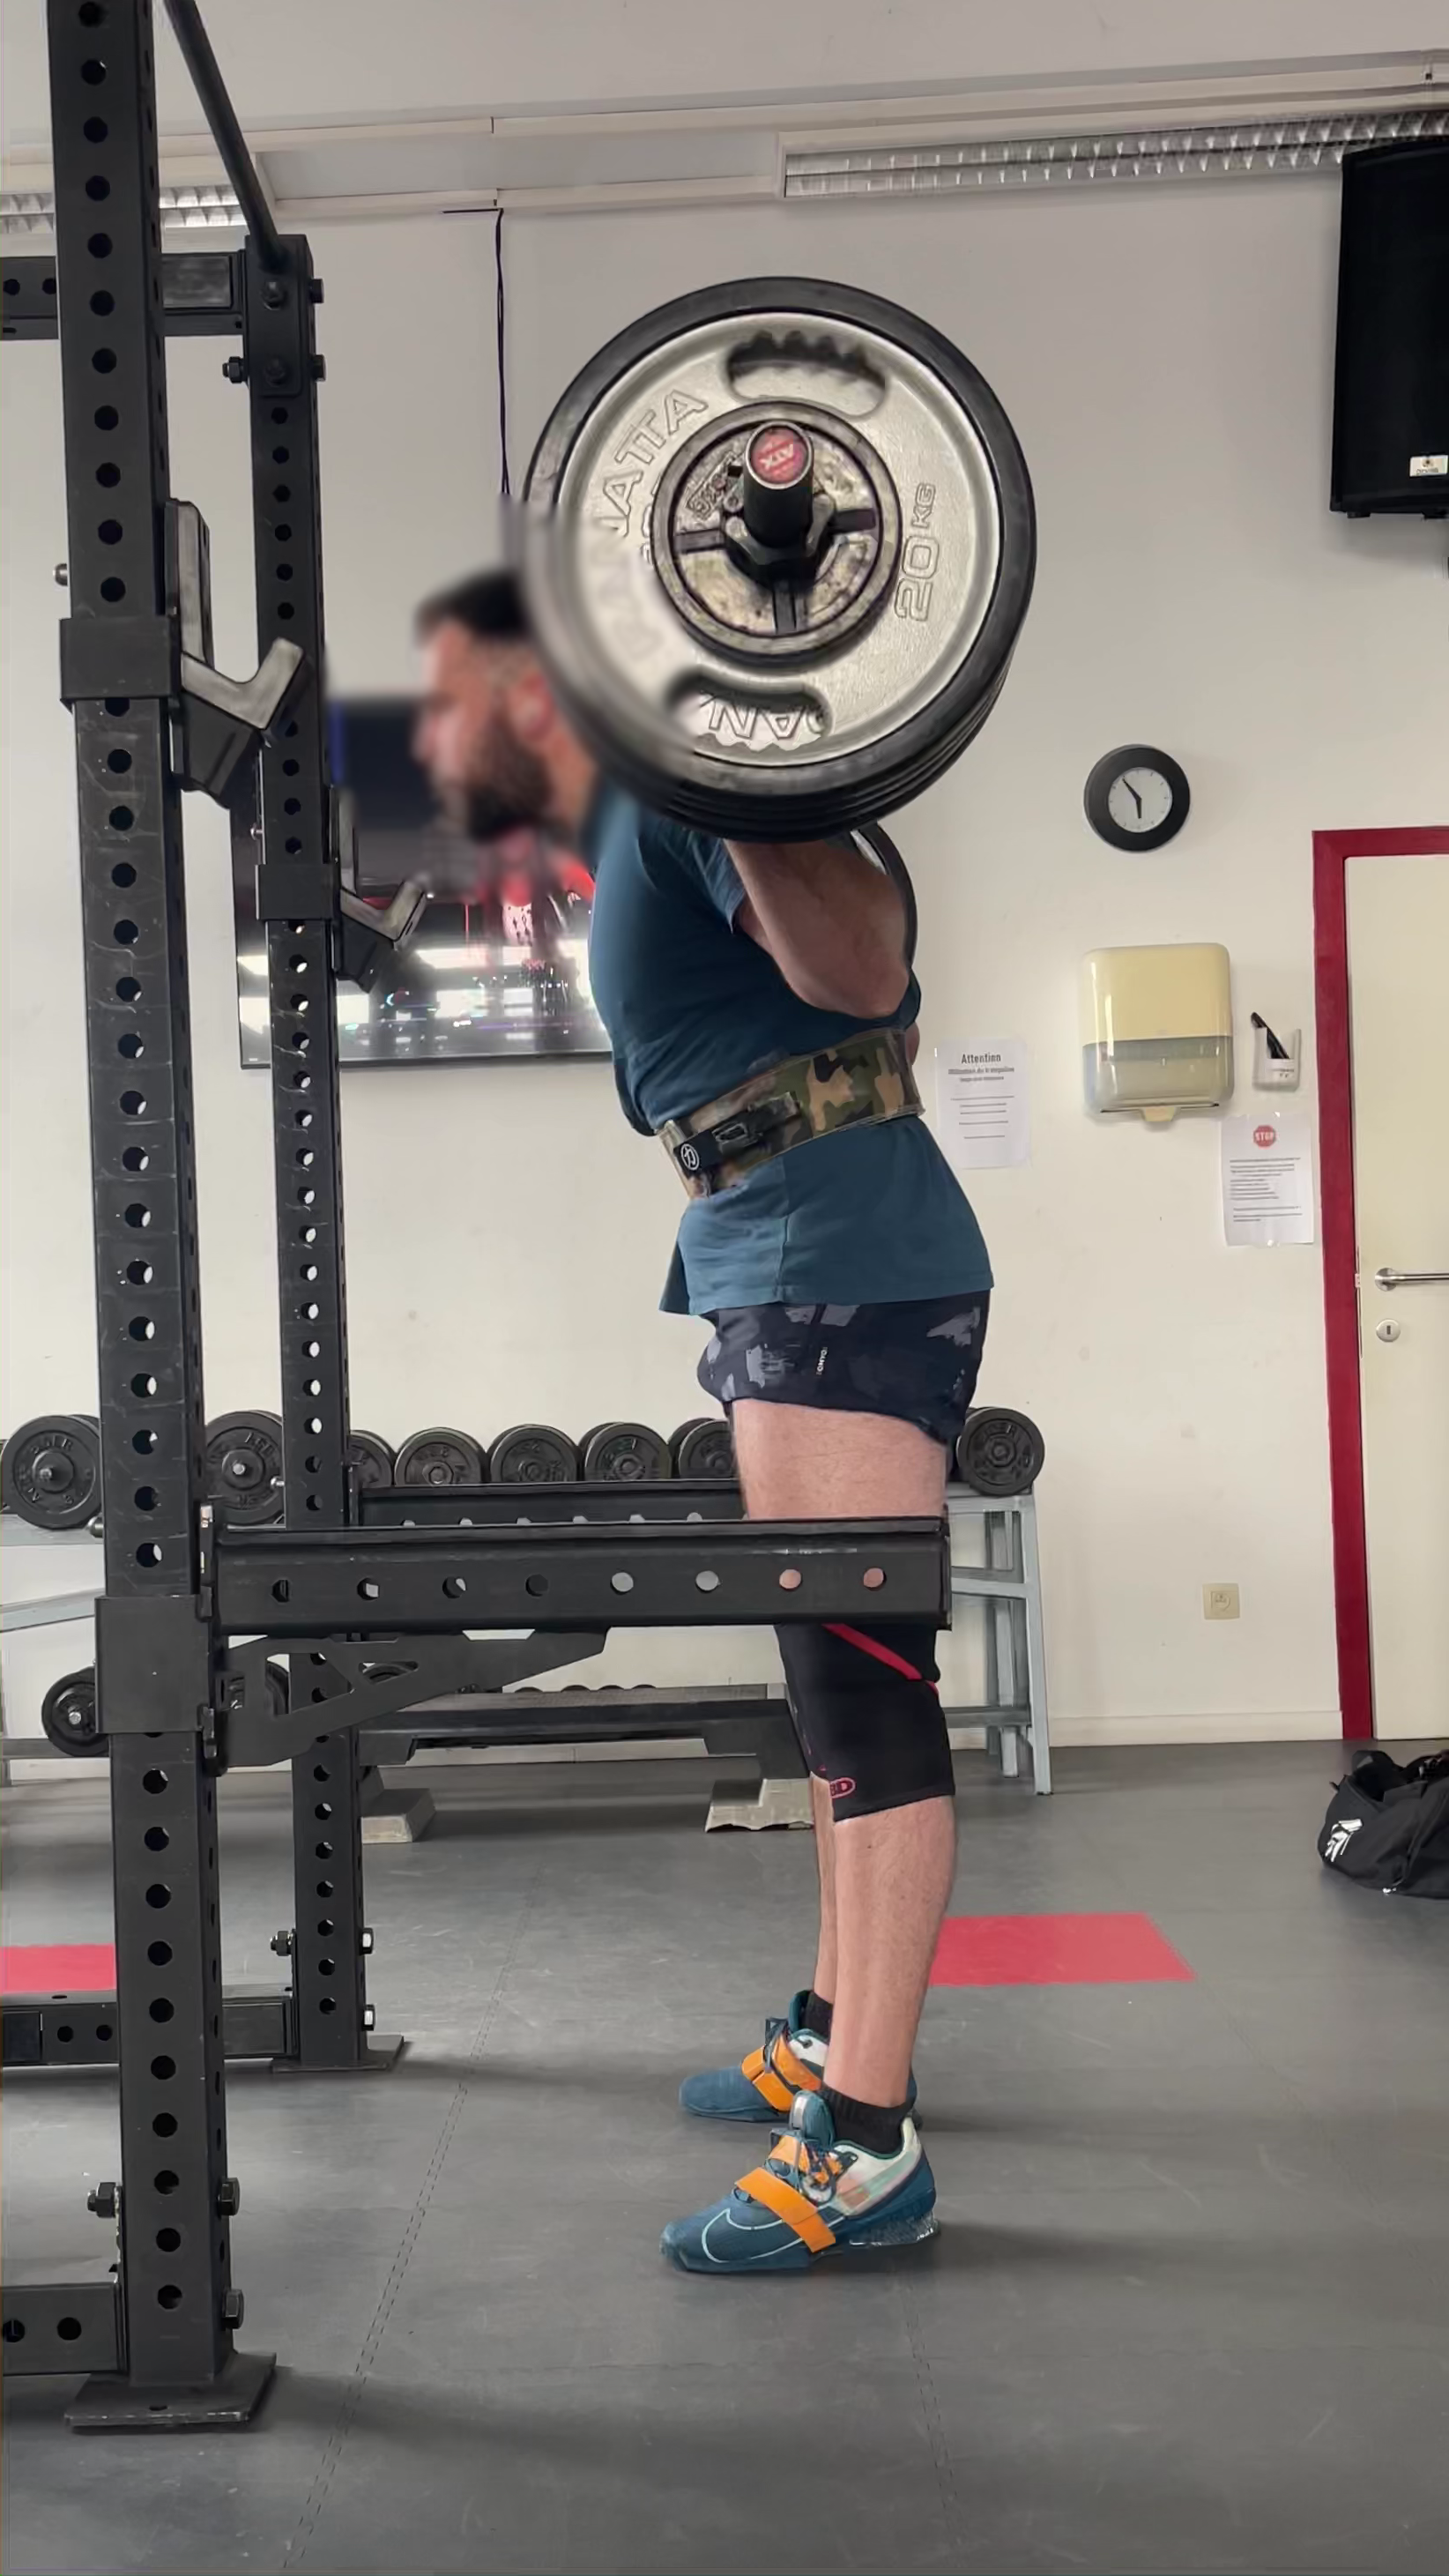
\includegraphics[width=3.5cm, height=5cm]{2-State_of_the_art/Squat.png}
  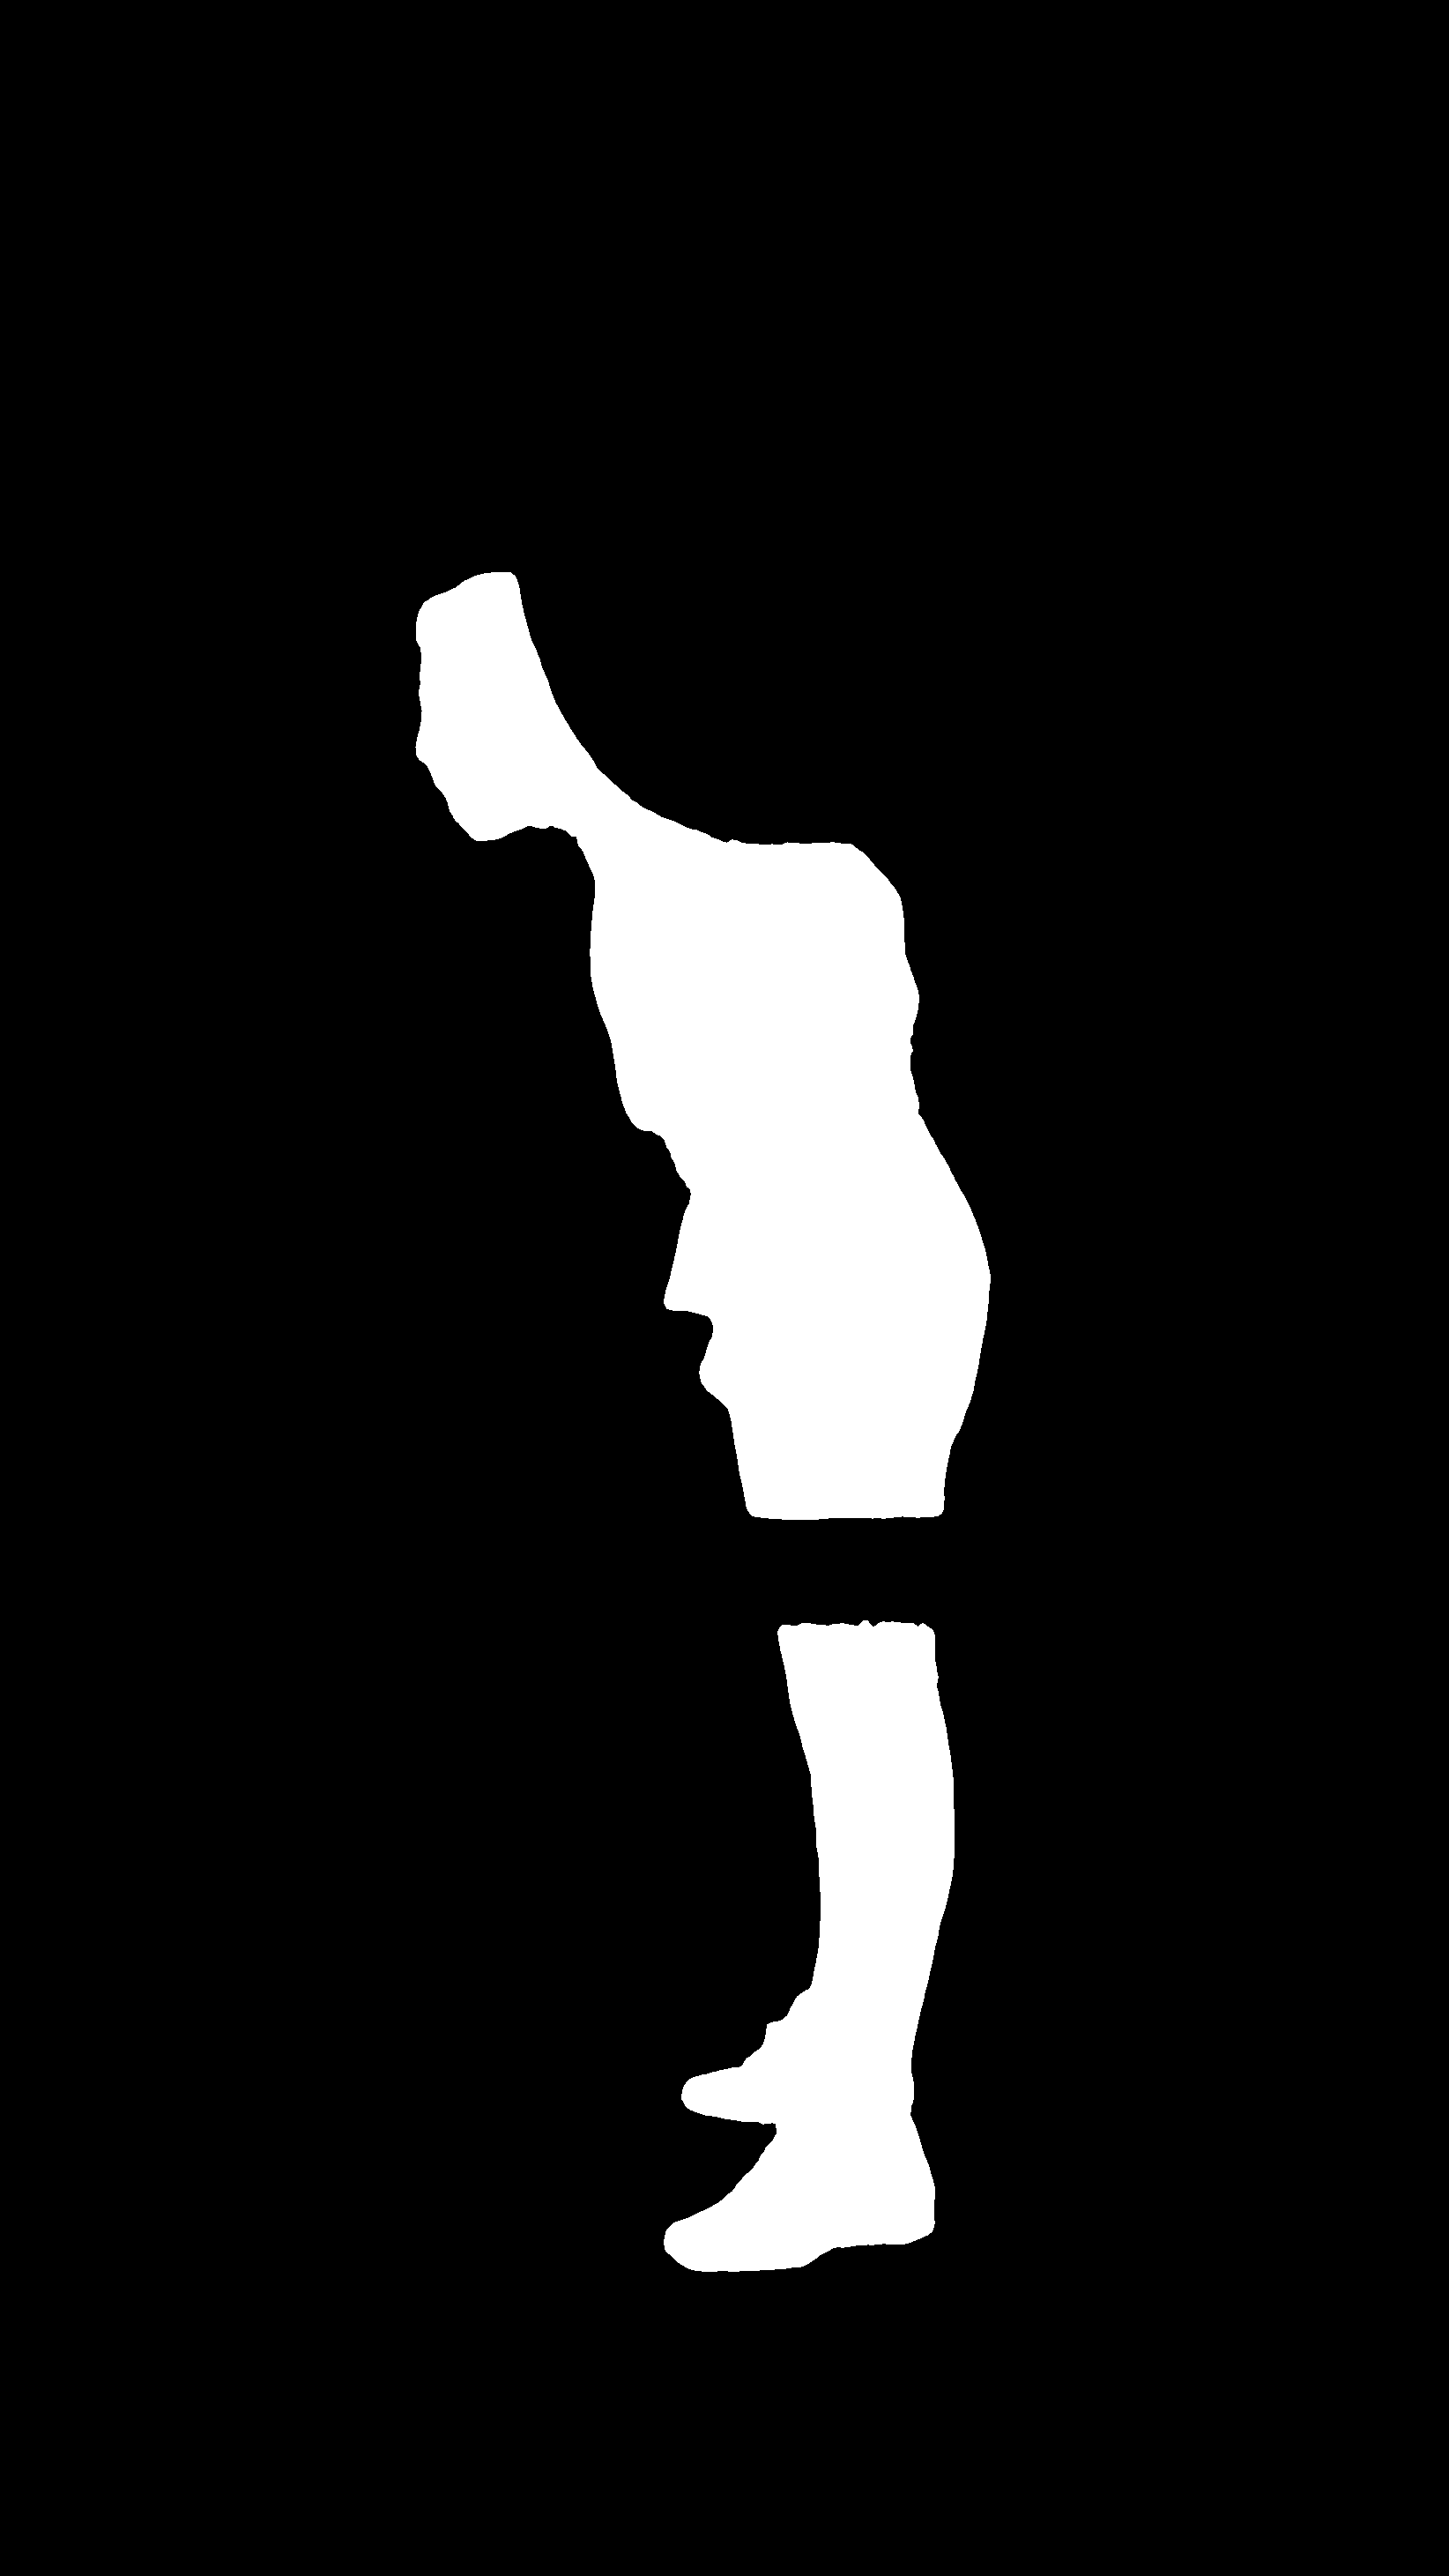
\includegraphics[width=3.5cm, height=5cm]{2-State_of_the_art/Squat-SAM3.png}
  \caption{Illustration de la segmentation}
  \label{fig:segment-illustration}
\end{figure}

\section{Estimation monoculaire de profondeur} 

L'estimation de profondeur monoculaire (\textit{Monocular Depth Estimation}, MDE) dérive une représentation tridimensionnelle à partir d'une matrice de pixels 2D. Les réseaux actuels, tels que Depth Anything (\textit{V1}~\cite{Depth-Anything-V1-2024} / \textit{V2}~\cite{Depth-Anything-V2-2024}) ou \textit{Monocular Geometry} (\textit{MoGe}~\cite{MoGe-2025} / \textit{MoGe2}~\cite{MoGe2-2025}), contournent le problème de la projection inverse \footnote{La projection inverse (\emph{inverse projection} ou \emph{back-projection}) désigne le problème consistant à retrouver les coordonnées tridimensionnelles d'un point de la scène à partir de sa projection bidimensionnelle sur le capteur.} en s'appuyant sur des informations apprises sur une vaste quantité de données hétérogènes. Ils extraient des cartes de profondeur denses, convertissant les intensités de pixels en valeurs métriques ou relatives (figure~\ref{fig:depth-estimation-illustration}). Cette construction spatiale est importante pour positionner correctement les segments corporels sur l'axe Z (profondeur) lors d'un mouvement capturé de face ou de trois-quarts.

\begin{figure}
  [htp]
  \centering
  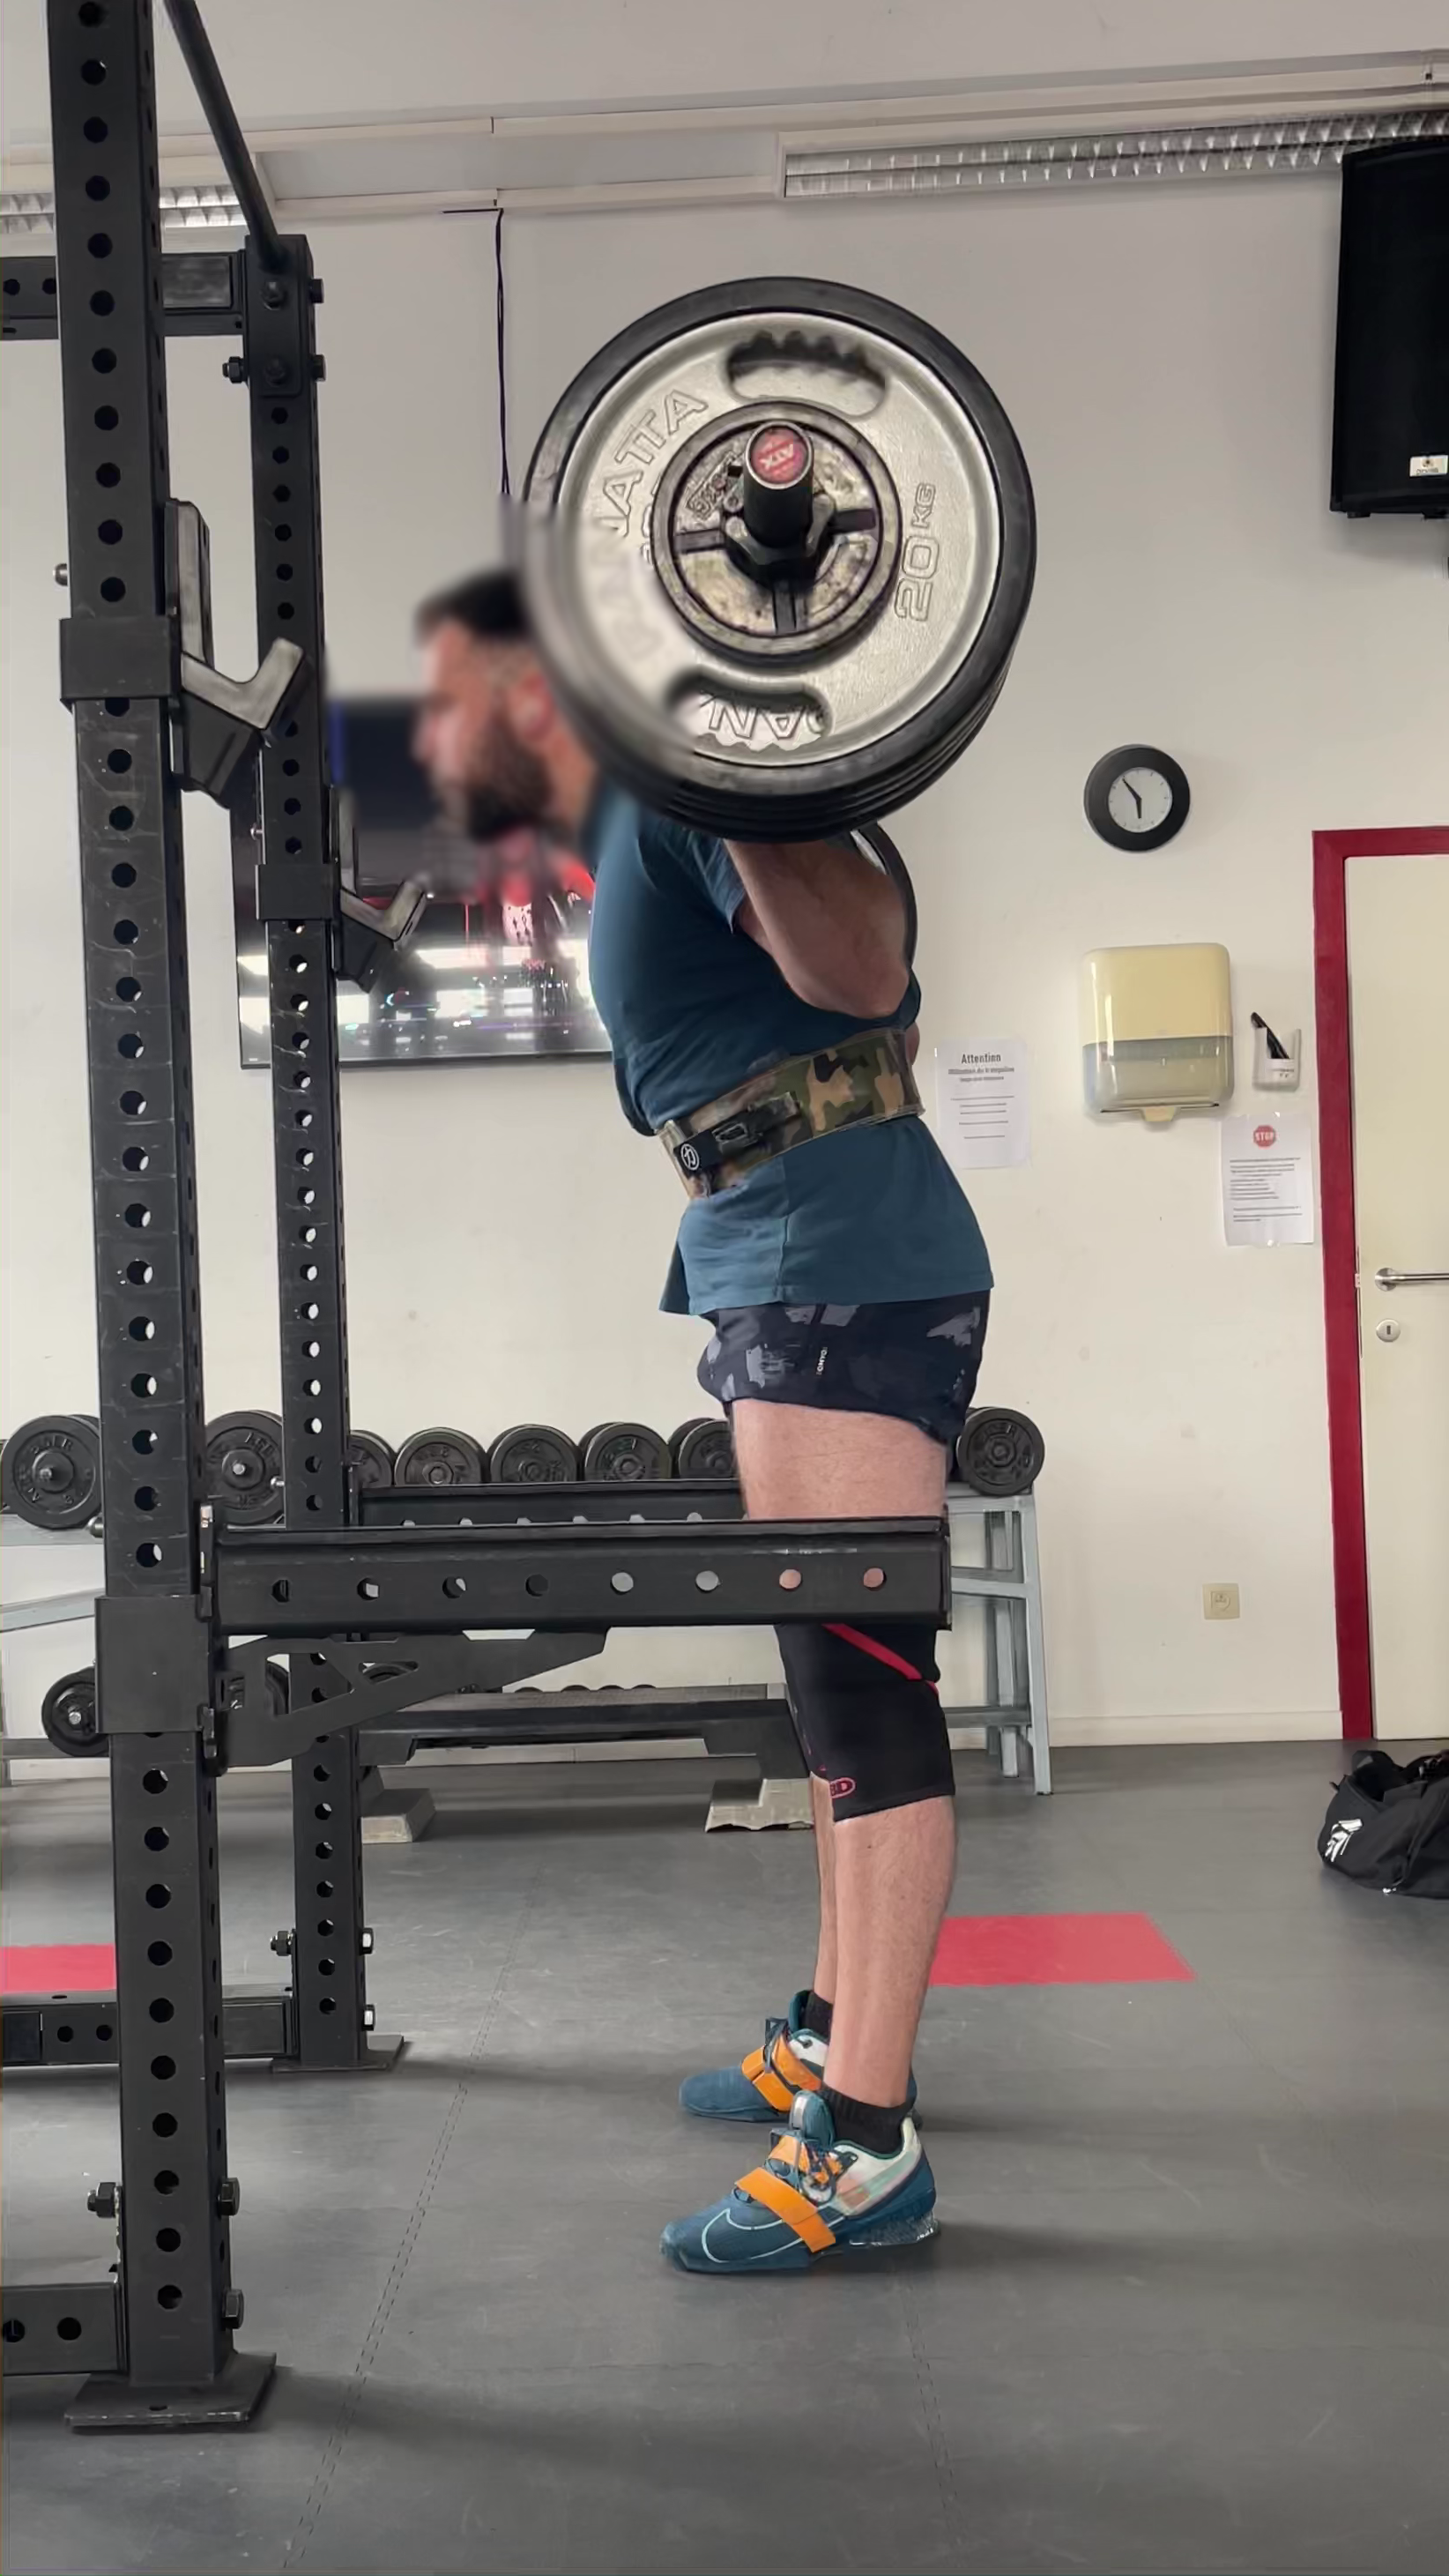
\includegraphics[width=3.5cm, height=5cm]{2-State_of_the_art/Squat.png}
  \includegraphics[width=3.5cm, height=5cm]{2-State_of_the_art/Squat-MoGe.png}
  \caption{Illustration de l'estimation de profondeur}
  \label{fig:depth-estimation-illustration}
\end{figure}

\section{Complétion amodale d'occlusions} 

L'occlusion matérielle partielle empêche le suivi cinématique. La complétion amodale vidéo (\textit{Video Amodal Completion}) vise à compléter de manière cohérente les structures manquantes (figure~\ref{fig:inpainting-illustration}). Les modèles génératifs de diffusion\footnote{Un modèle génératif de diffusion (\emph{diffusion model}) est un modèle probabiliste (c'est-à-dire qui ne produit pas une sortie déterministe unique, mais modélise une distribution de probabilité sur les sorties possibles) qui apprend à générer des données en simulant un processus de débruitage itératif.}, spécifiquement des architectures comme TACO (\textit{Taming Diffusion for in-the-wild Video Amodal Completion})~\cite{TACO-2025}, permettent un débruitage itératif via les trames et les masques de segmentation préalablement extraits. Cette opération synthétise les pixels occlus (par exemple : par un rack ou par un disque de poids) en maintenant la continuité temporelle. Cette reconstruction préventive fournit au module d'estimation de pose 3D une topologie corporelle complète, diminuant les erreurs d'inférence.

\begin{figure}
  [htp]
  \centering
  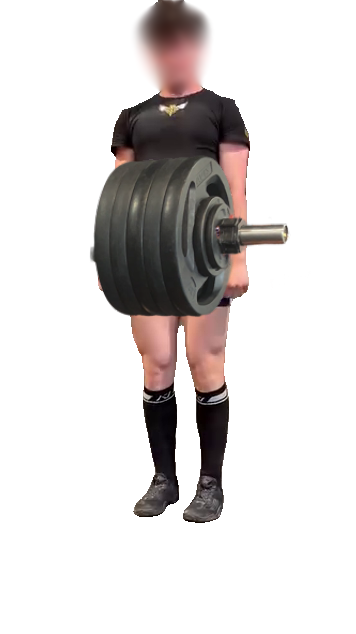
\includegraphics[width=3.5cm, height=5cm]{2-State_of_the_art/Deadlift-occlusion.png}
  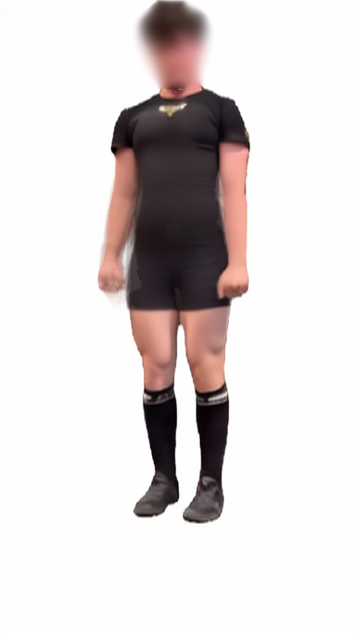
\includegraphics[width=3.5cm, height=5cm]{2-State_of_the_art/Deadlift-lora.png}
  \caption{Illustration de la complétion amodale d'occlusions}
  \label{fig:inpainting-illustration}
\end{figure}

\section{Estimation de pose 2D et 3D} \label{sec:2d-3d-estimation}

L'estimation de pose humaine (\textit{Human Pose Estimation}) consiste à localiser les points articulaires d'un individu. Deux grandes familles de méthodes se distinguent selon la dimensionnalité de la représentation produite : les approches bidimensionnelles, qui opèrent dans le plan image, et les approches tridimensionnelles, qui cherchent à restituer la géométrie complète du corps dans l'espace.

\textbf{Les approches 2D} : Les architectures historiques comme HRNet (\textit{High-Resolution Net})~\cite{HRNet-2019} ou OpenPose~\cite{OpenPose-2019} constituent les fondations du domaine. OpenPose en particulier présente des limitations face aux occlusions~\cite{OpenPose-2019} : les keypoints occultés étant généralement absents des annotations d'entraînement, le modèle produit des faux négatifs et une précision de localisation dégradée dès qu'un membre disparaît du champ visuel~\cite{OpenPose-2019}. De plus, dans les scènes où plusieurs personnes se chevauchent, son mécanisme d'assemblage multi-personnes tend à fusionner les annotations de sujets distincts, produisant des squelettes anatomiquement incohérents~\cite{OpenPose-2019}. L'état de l'art actuel s'appuie sur les transformeurs de vision (par exemple : ViTPose~\cite{ViTPose-2022}, ViTPose++~\cite{ViTPose++-2024}) et les modèles unifiés temps réel \footnote{Les modèles unifiés temps réel désignent des architectures conçues pour effectuer simultanément la détection d'objets et l'estimation de pose en une seule passe réseau. Cette conception permet d'atteindre des fréquences d'inférence compatibles avec le traitement vidéo en direct, typiquement supérieures à 30 images par seconde.} (par exemple : YOLO-Pose~\cite{YOLO-Pose-2022}) afin accroître la robustesse de l'inférence. Bien qu'elles extraient des coordonnées bidimensionnelles avec une bonne précision face aux occlusions, ces méthodes demeurent intrinsèquement limitées par la perte d'information spatiale et les erreurs de parallaxe (par exemple : l'inclinaison du buste vers l'avant modifiant la projection visuelle des segments articulaires). Ces limitations sont particulièrement problématiques dans le contexte de la force athlétique, où la barre et les disques génèrent des occlusions massives et prolongées sur des régions articulaires clés, motivant le recours à un pipeline de complétion amodale en amont de l'estimation de pose.

\textbf{Les approches 3D} : Le passage à la dimension supérieure s'effectue soit par levée d'ambiguïté directe depuis l'image (via des modèles de régression), soit par triangulation si plusieurs vues sont disponibles. Dans un contexte monoculaire, le défi de l'estimation de la profondeur relative \footnote{La profondeur relative désigne la distance d'un point de la scène par rapport à la caméra. En vision monoculaire, cette estimation est ambiguë car une infinité de scènes tridimensionnelles distinctes peuvent produire la même projection bidimensionnelle sur le capteur (ambiguïté de profondeur). Les modèles d'apprentissage profond cherchent à lever cette ambiguïté en s'appuyant sur des indices monoculaires appris : texture, perspective, taille relative des objets et relations spatiales entre segments corporels.} est résolu par l'intégration de modèles paramétriques du corps humain. Historiquement centrés sur le modèle SMPL (\textit{Skinned Multi-Person Linear model})~\cite{SMPL-2015} et ses évolutions expressives (SMPL-X~\cite{SMPL-X-2019}) sont aujourd'hui concurrencés par des architectures de nouvelle génération comme le MHR (\textit{Momentum Human Rig})~\cite{MHR-2025} de Meta. MHR redéfinit la modélisation paramétrique en séparant strictement le squelette et la forme. Cette structure découplée garantit une meilleure plausibilité biomécanique et une fidélité supérieure (figure~\ref{fig:pose-estimation-illustration}).

\begin{figure}
  [htp]
  \centering
  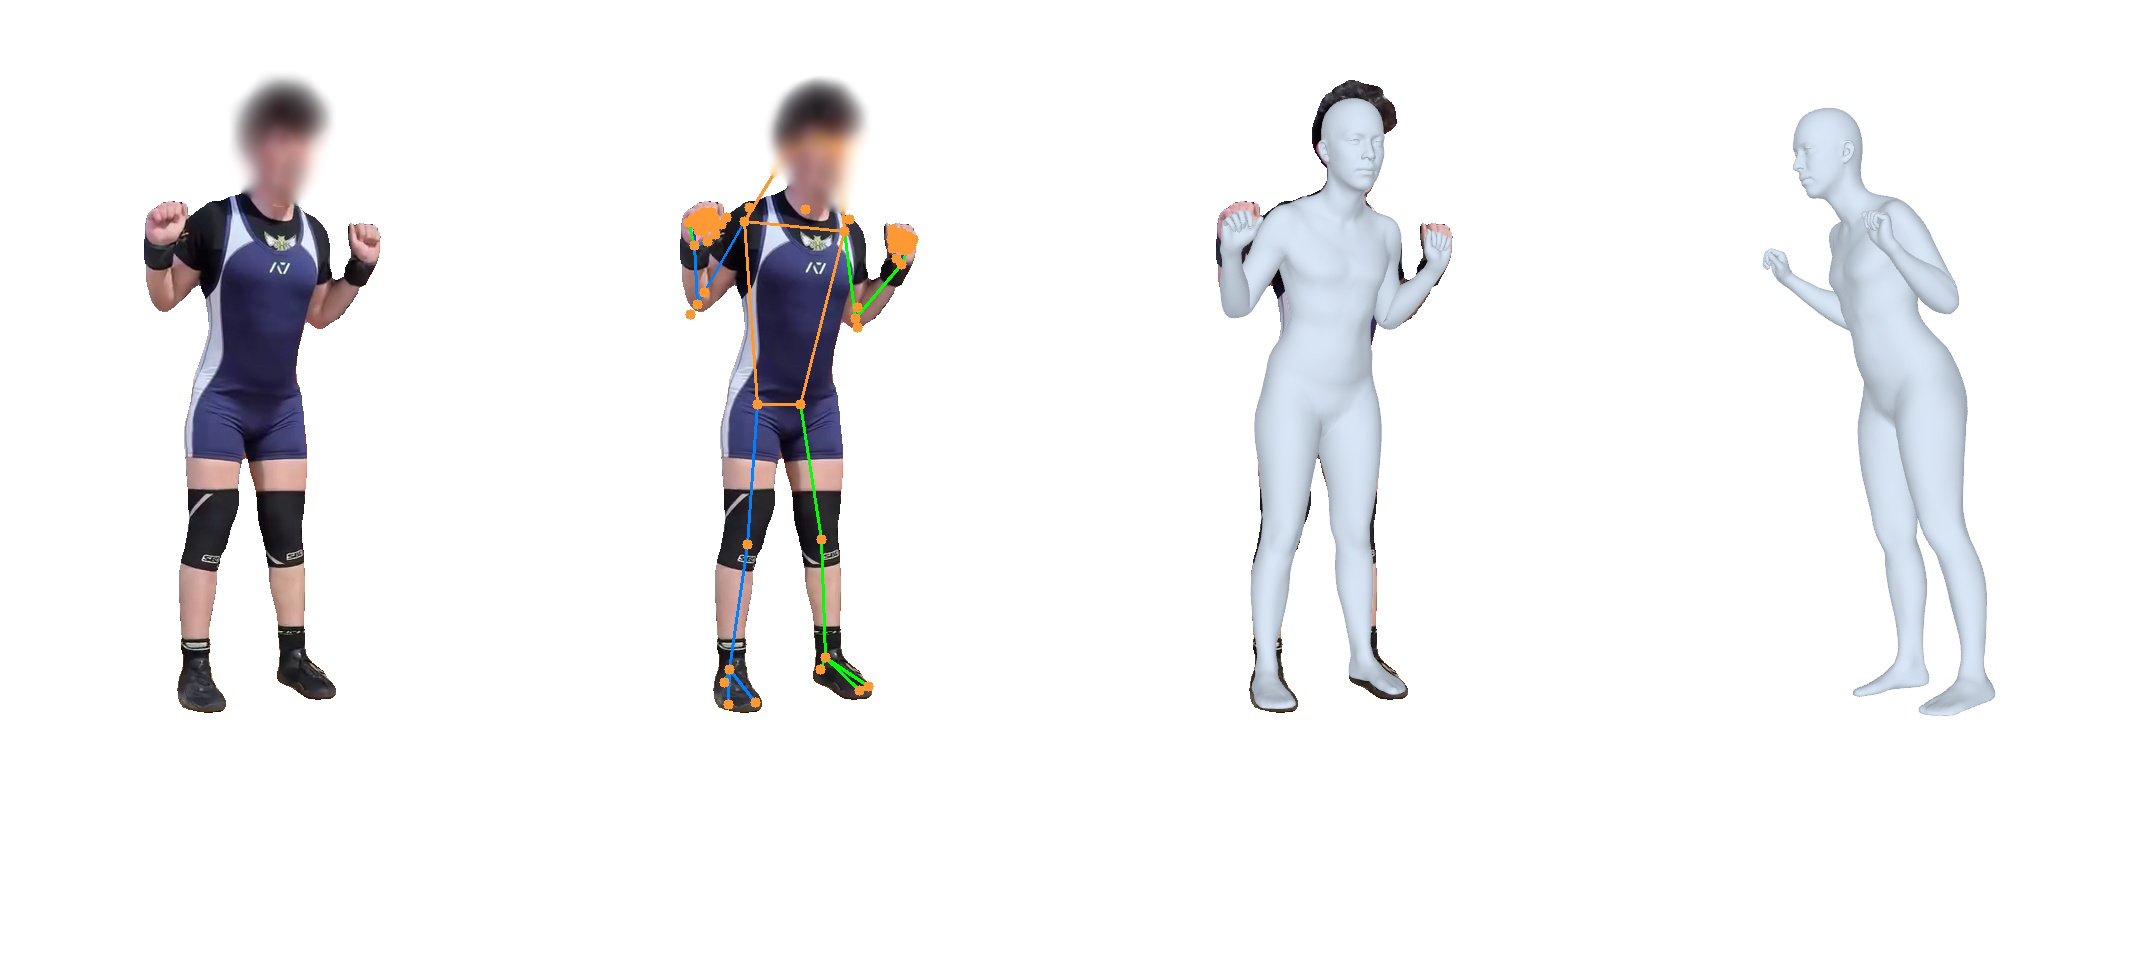
\includegraphics[width=12cm, height=5cm]{2-State_of_the_art/Squat-SMA3DBody.jpg}
  \caption{Illustration de l'estimation de pose}
  \label{fig:pose-estimation-illustration}
\end{figure}

% ---------------------
% ARCHITECTURE DU PIPELINE
% ---------------------
\chapter{Architecture du pipeline} \label{ch_three}

\section{Vue d'ensemble et flux de données}

Le pipeline développé dans ce mémoire vise à reconstruire un modèle 3D complet du corps d'un individu à partir d'une vidéo monoculaire d'entraînement, typiquement filmée dans une salle de musculation où l'environnement est encombré (machines, autres individus, miroirs, équipements) et où le sujet est fréquemment partiellement occulté par la barre, les disques, ou les structures de sécurité. Le fait que les vidéos soient captées sans contrôle de la prise de vue, de l'éclairage, ni du fond, impose un enchaînement de modules capables de gérer l'identification du sujet d'intérêt et la complétion d'informations manquantes.

L'architecture proposée est modulaire et séquentielle. Elle s'organise autour de quatre modules principaux fondés sur des modèles de l'état de l'art (SAM3, MoGe-2, TACO, SAM 3D Body), complétés par deux étapes de traitement intermédiaires (filtre de profondeur et isolation du sujet). La figure~\ref{fig:ai-pipeline} en présente la vue d'ensemble.

\begin{figure}[htp]
  \centering
  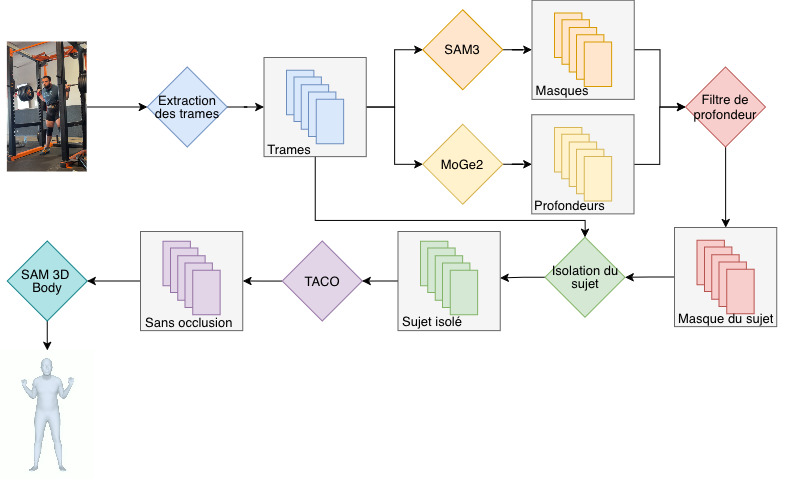
\includegraphics[height=9.5cm]{images/3-Pipeline_architecture/Pipeline.jpg}
  \caption{Vue d'ensemble du pipeline}
  \label{fig:ai-pipeline}
\end{figure}

Le flux de données peut être décrit comme suit :

\begin{enumerate}
  \item La vidéo d'entrée est d'abord décomposée en une séquence d'images individuelles (\textit{trames}).
  \item Deux traitements parallèles sont ensuite appliqués sur chaque image :
  \begin{itemize}
    \item \textbf{SAM3}~\cite{SAM3-2025} génère un ensemble de masques de segmentation correspondant à toutes les personnes présentes dans la scène.
    \item \textbf{MoGe-2}~\cite{MoGe2-2025} produit une carte de profondeur, attribuant à chaque pixel une estimation de sa distance par rapport à la caméra.
  \end{itemize}
  \item Un \textbf{filtre de profondeur} fusionne ces deux sorties pour ne conserver que les masques correspondants au sujet situé au premier plan, écartant ainsi les autres personnes situées en arrière-plan.
  \item L'étape d'\textbf{isolation du sujet} applique ces masques filtrés sur les images originales, produisant une séquence où seul le sujet apparaît sur un fond neutre (blanc).
  \item Ces images sont ensuite traitées par \textbf{TACO}~\cite{TACO-2025}, un modèle de complétion amodale vidéo qui reconstruit les parties du sujet occultées par les équipements (barres, disques, machines), tout en garantissant la cohérence temporelle entre les trames.
  \item Enfin, \textbf{SAM 3D Body}~\cite{SAM-3D-Body-2026} reçoit en entrée la séquence d'images ne présentant plus d'occlusions et reconstruit la pose ainsi que la forme corporelle caractérisant la morphologie de l'individu.
\end{enumerate}

Ce choix d'architecture séquentielle est motivé par plusieurs considérations. D'une part, bien que des approches unifiées telles qu'OpenPose~\cite{OpenPose-2019} ou ViTPose~\cite{ViTPose-2022} permettent d'estimer un squelette 3D et présentent une certaine robustesse aux occlusions partielles, elles demeurent insuffisantes dans notre contexte pour deux raisons. Premièrement, leur robustesse aux occlusions se dégradent face aux occlusions massives et prolongées (voir section~\ref{sec:2d-3d-estimation}), ces occlusions sont caractéristiques des vidéos de force athlétique. Deuxièmement, aucun modèle unique disponible publiquement ne couvre conjointement l'intégralité de la chaîne de traitement requise : isolation du sujet dans un environnement encombré, estimation de profondeur, complétion amodale temporellement cohérente et reconstruction d'un maillage corporel complet. D'autre part, le découpage modulaire permet de remplacer indépendamment chaque composant lorsque de nouveaux modèles plus performants émergent, un point particulièrement pertinent compte tenu du rythme actuel des publications dans le domaine de la vision par ordinateur. Enfin, cette structure offre une meilleure interprétabilité du système, en cas d'erreur en sortie, il est possible d'identifier précisément le module posant problème.

\section{Module 1 : Segmentation avec SAM3} \label{sec:module-1}

\subsection{Principe et architecture}

SAM3 (\textit{Segment Anything Model 3}), publié par Meta en novembre 2025~\cite{SAM3-2025}, est un modèle de segmentation fondationnel introduisant la notion de \textit{Promptable Concept Segmentation} (PCS). Pour comprendre l'apport de SAM3, il est important de rappeler le fonctionnement de ses prédécesseurs. SAM et SAM2 opèrent à partir d'un prompt interactif localisé (un point, une boîte englobante ou un masque grossier) et produisent un unique masque correspondant à l'objet pointé. L'utilisateur  doit donc interagir manuellement avec chaque instance qu'il souhaite segmenter. SAM3 n'utilise plus seulement ce paradigme mais introduit la notion de prompt textuel. Plutôt que de pointer un objet précis, l'utilisateur spécifie une catégorie (par exemple \emph{"human"}) via un prompt textuel. Le modèle détecte alors automatiquement toutes les instances correspondant à ce prompt dans l'image ou la vidéo, et génère un masque pour chacune d'elles, sans intervention manuelle. Dans le pipeline, cette propriété est exploitée pour isoler l'ensemble des personnes présentes dans la scène en une seule inférence, le filtre de profondeur permettra ensuite de sélectionner le sujet d'intérêt au premier plan.

L'architecture repose sur un transformeur double encodeur-décodeur \footnote{Un transformeur double encodeur-décodeur désigne une architecture composée de deux branches parallèles : un encodeur qui extrait des représentations sémantiques de haut niveau depuis l'image d'entrée, et un décodeur qui reconstruit progressivement la sortie depuis ces représentations. Le qualificatif \textit{double} indique que l'architecture dispose de deux paires encodeur-décodeur spécialisées.}. Plus précisément, elle découple un détecteur de type DETR (\textit{DEtection TRansformer}) d'un suiveur vidéo dérivé de SAM2, auquel s'ajoute une "\textit{presence head}" destinée à stabiliser le suivi d'instance sur de longues séquences. Le modèle a été entraîné sur le jeu de données (\textit{dataset}) SA-Co~\cite{SAM3-SA-Co-2025} qui est un dataset de référence pour la segmentation d'objets dans les images, cet ensemble de données contient des images associées à des étiquettes textuelles. SAM3 a atteint une précision moyenne pour des masques de segmentation \textit{zero-shot} de 47.0 mAP (\textit{mean Average Precision}) \footnote{"mean Average Precision" est une métrique globale de la performance d'un modèle de détection d'objets, prenant en compte la précision pour chaque classe d'objet présente dans les prédictions, elle s'exprime sur une échelle allant de 0 à 1 (ou 0\% à 100\%).} sur LVIS~\cite{LVIS-Dataset-2019}, qui est un dataset de référence pour la détection d'objets, contre 38.5 mAP pour le précédent état de l'art. 


\subsection{Entrées et sorties dans le pipeline}

Dans le pipeline, SAM3 est appliqué trame par trame avec un prompt textuel orienté vers la détection de toutes les personnes. Pour chaque trame, SAM3 produit un ensemble de masques binaires correspondant aux personnes détectées, la trame étant traitée indépendamment des trames voisines. Le tracker vidéo intégré à SAM3, bien que disponible, n'est pas exploité dans l'implémentation effectuée en raison de la mémoire GPU requise pour maintenir l'état de tracking sur des séquences longues, incompatible avec la contrainte d'inférence sur les GPU mis à disposition durant le mémoire (voir section~\ref{sec:integration}).

Ce traitement indépendant trame par trame implique que les identifiants d'instance produits par SAM3 ne sont pas cohérents temporellement, le masque associé au sujet à la trame $t$ peut porter l'indice $i$ et celui correspondant au même sujet à la trame $t+1$ porter un indice $j \neq i$. La continuité d'identité est rétablie par la suite via le filtre de profondeur (section~\ref{sec:filtre-profondeur}), qui filtre à chaque trame le masque de la personne la plus proche. Cette stratégie est robuste tant que le sujet d'intérêt reste le plus proche de la caméra, hypothèse vérifiée dans la quasi-totalité des contextes de musculation où l'individu est filmé en premier plan, les autres pratiquants étant systématiquement plus éloignés de la caméra.

\subsection{Justification du choix}

Deux propriétés ont motivé le choix de SAM3 sur d'autres modèles de segmentation candidats (Mask R-CNN~\cite{Mask-R-CNN-2018}, DETR~\cite{DETR-2020}, YOLOv11-seg~\cite{Ultralytics-YOLO-2026}, SAM2~\cite{SAM2-2024}) :

\begin{itemize}
  \item \textbf{Robustesse \textit{zero-shot}.} L'environnement d'une salle de musculation contient des objets atypiques (machines spécifiques, vêtements de sport variés, équipements rares) qui ne figurent pas systématiquement dans les jeux de données classiques. La capacité de SAM3 à généraliser sans fine-tuning évite une coûteuse et longue phase de réannotation.
  \item \textbf{Promptabilité conceptuelle.} La possibilité de cibler explicitement le concept \emph{"personne"} par simple texte simplifie considérablement l'intégration dans le pipeline.
\end{itemize}

\subsection{Limites et alternatives}

SAM3 présente toutefois plusieurs limites dans notre contexte. Premièrement, la latence d'inférence reste élevée sur du matériel local : alors que les auteurs rapportent environ 30 ms par image sur GPU H200, le temps d'inférence observé sur notre configuration (NVIDIA RTX
A5000, 24 Go GDDR6) est nettement supérieur (environ 200 ms, mesuré expérimentalement sur la station de travail) en raison de la moindre puissance de calcul de la RTX A5000 par rapport au GPU H200 utilisé par les auteurs. Ce point exclut toute exécution en temps réel sur ce matériel et impose un traitement en post-production. Deuxièmement, le modèle peut produire des masques fragmentés lorsque le sujet est partiellement occulté par un objet de couleur similaire (par exemple un t-shirt noir devant un fond noir), nécessitant un post-traitement morphologique (fermeture suivie d'une sélection de la composante connexe principale). Troisièmement, en cas de présence de plusieurs personnes proches dans le champ, la sélection automatique du sujet d'intérêt requiert le filtre de profondeur décrit en section~\ref{sec:filtre-profondeur}. Enfin, l'absence d'exploitation du tracker vidéo intégré (justifiée précédement) impose de reconstruire la continuité d'identité par la suite, ce qui peut occasionnellement échouer lorsque par exemple deux personnes se croisent à des profondeurs similaires.

Des alternatives ont été considérées et écartées :
\begin{itemize}
  \item \textbf{SAM2} fournit une excellente segmentation interactive mais ne permet pas de détecter spontanément toutes les instances d'un concept par prompt textuel.
  \item \textbf{Grounded-SAM} combine GroundingDINO et SAM en deux passes séquentielles (détection textuelle puis segmentation) ce qui double le temps d'inférence par rapport à un modèle unifié.
  \item \textbf{YOLOv11-seg} offre une latence très faible mais ses masques sont moins précis que SAM3. Cette imprécision dégraderait la précision du filtre de profondeur, qui calcule la profondeur du sujet sur la base de son masque. Un masque grossier inclurait des pixels d'arrière-plan proches du sujet, biaisant l'estimation lorsque plusieurs personnes apparaissent à des profondeurs comparables.
\end{itemize}

\section{Module 2 : Carte de profondeur avec MoGe-2} \label{sec:module-2}

\subsection{Principe et architecture}

MoGe-2 (\emph{Monocular Geometry estimation v2}) est un modèle d'estimation de géométrie monoculaire publié en 2025 par Microsoft~\cite{MoGe2-2025}. Là où l'estimation de profondeur classique se limite à prédire un scalaire par pixel, MoGe-2 prédit directement un \emph{point map} 3D métrique, c'est-à-dire l'association de chaque pixel à un point $(X, Y, Z)$ exprimé dans un repère avec une échelle réelle.

MoGe-2 repose sur une architecture de type encodeur-décodeur fondée sur un transformeur de vision (\textit{Vision Transformer}) pré-entraîné. Le modèle a été entraîné sur un corpus hétérogène massif combinant des données réelles issues de scanners LiDAR \footnote{Le LiDAR (\emph{Light Detection And Ranging}) est un capteur qui mesure la distance par rapport aux objets en émettant des impulsions laser et en mesurant le temps de retour de l'écho. Il produit un nuage de points 3D dense, constituant une vérité terrain de profondeur précise au centimètre.} et de capteurs RGB-D\footnote{Un capteur RGB-D (Red Green Blue - Depth) est un dispositif combinant une caméra couleur standard et un capteur de profondeur (typiquement infrarouge). Il produit simultanément une image couleur et une carte de profondeur alignée pixel à pixel, fournissant ainsi une représentation 2,5D de la scène.}, des données synthétiques générées par rendu 3D, ainsi que des pseudo-vérités terrain produites par des méthodes de reconstruction multi-vues. Cette diversité des sources d'entraînement est la clé de sa capacité de généralisation \textit{zero-shot} : des estimations métriques cohérentes sont produites sur des images non vues lors de l'entraînement, sans calibration préalable de la caméra. Dans le pipeline présenté dans ce mémoire, cette propriété est exploitée pour stratifier spatialement la scène et isoler l'athlète au premier plan par un filtre de profondeur.

L'architecture combine deux innovations majeures par rapport au modèle original MoGe :

\begin{enumerate}
  \item Une représentation hybride associant un point map (héritage de MoGe) à un facteur d'échelle global~\cite{MoGe-2025}, ils sont prédits séparément, ce découplage permet de bénéficier de la qualité géométrique offerte par la prédiction tout en récupérant l'échelle métrique réelle, contournant ainsi l'ambiguïté focale-distance \footnote{En vision monoculaire, la distance d'un objet à la caméra et la longueur focale de l'objectif produisent des effets sur la projection 2D : un objet lointain capturé avec un téléobjectif produit la même image qu'un objet proche capturé avec un grand-angle. Sans connaissance préalable de la focale, il est donc impossible de récupérer l'échelle métrique absolue depuis une seule image.}.
  \item Une stratégie de raffinage des données d'entraînement (\textit{data refinement}) qui filtre et complète les annotations bruitées des jeux de données réels en s'appuyant sur des labels synthétiques. Cette procédure améliore significativement la finesse des contours sans dégrader la précision globale.
\end{enumerate}

Le modèle prédit aussi le point map, la profondeur dérivée et le champ de vision (\textit{FOV}) de la caméra, ce qui est particulièrement utile dans un contexte où les métadonnées de capture sont souvent indisponibles, comme c'est le cas pour les vidéos d'entraînement filmées par des pratiquants amateurs.

\subsection{Entrées et sorties dans le pipeline}

MoGe-2 est appliqué indépendamment à chaque trame et produit une carte de profondeur métrique. À chaque pixel est associée une distance exprimée en mètres. Cette carte est ensuite passée au filtre de profondeur (section~\ref{sec:filtre-profondeur}) pour identifier les pixels appartenant au sujet de premier plan. Le seuil de séparation entre premier plan et arrière-plan n'est pas fixé manuellement : il est estimé automatiquement à partir de la distribution des profondeurs dans la carte, en identifiant le pic de profondeur minimal correspondant au sujet le plus proche de la caméra. Cette approche adaptive dispense de toute calibration préalable et reste valide quelle que soit la distance entre l'athlète et la caméra.

\subsection{Justification du choix}

Plusieurs modèles de profondeur monoculaire étaient candidats : MiDaS~\cite{MiDaS-2020}, ZoeDepth~\cite{ZoeDepth-2023}, Depth Anything V2~\cite{Depth-Anything-V2-2024}, Marigold~\cite{Marigold-2024}, UniDepth~\cite{UniDepth-2024}, et MoGe-2~\cite{MoGe2-2025}. Le choix s'est porté sur MoGe-2 pour les raisons suivantes :

\begin{itemize}
  \item \textbf{Échelle métrique native.} Contrairement à MiDaS ou Depth Anything qui produisent une profondeur relative, MoGe-2 fournit directement des valeurs métriques exploitables pour le filtrage spatial.
  \item \textbf{Précision sur les contours.} La stratégie de raffinement des données conduit à des silhouettes humaines nettement plus précises que les concurrents~\cite{MoGe2-2025}, ce qui est important pour éviter qu'un pixel du sujet ne soit attribué au fond (ou inversement) lors de la combinaison avec les masques SAM3.
  \item \textbf{Robustesse open-domain.} Le modèle a été entraîné sur un corpus de 24 jeux de données~\cite{MoGe2-2025} totalisant environ 8,9 millions de trames, combinant trois types de sources : des données réelles issues de scanners LiDAR, des reconstructions SfM (\textit{Structure from Motion})\footnote{La reconstruction \emph{Structure from Motion} (SfM) est une technique de vision par ordinateur permettant de reconstruire une scène 3D et la trajectoire de la caméra à partir d'un ensemble d'images 2D prises sous différents angles.} en environnements intérieurs comme extérieurs, et des données synthétiques. Cette diversité garantit une généralisation robuste à des environnements non vus lors de l'entraînement, comme les salles de sport.
\end{itemize}

\subsection{Limites et alternatives} \label{subsec:background-limitation}

Dans les salles de musculation fréquentées, d'autres individus peuvent apparaître dans le champ de la caméra. Lorsque leurs vêtements présentent une couleur ou une luminosité similaire à ceux du sujet d'intérêt, le filtre de profondeur peut échouer à les différencier correctement. La figure~\ref{fig:background-limitation} illustre ce cas : un second pratiquant en tenue claire, visible en arrière-plan, est partiellement fusionné avec la main du sujet principal dans le masque produit par SAM3. Le filtre de profondeur, qui s'appuie sur la profondeur médiane du masque pour identifier le sujet au premier plan, est mis en échec lorsque les deux silhouettes se chevauchent visuellement à des profondeurs pourtant distinctes. La reconstruction TACO reçoit alors une silhouette étendue incluant des pixels appartenant à l'autre pratiquant, introduisant des artefacts dans les régions concernées.

\begin{figure}[htp]
  \centering
  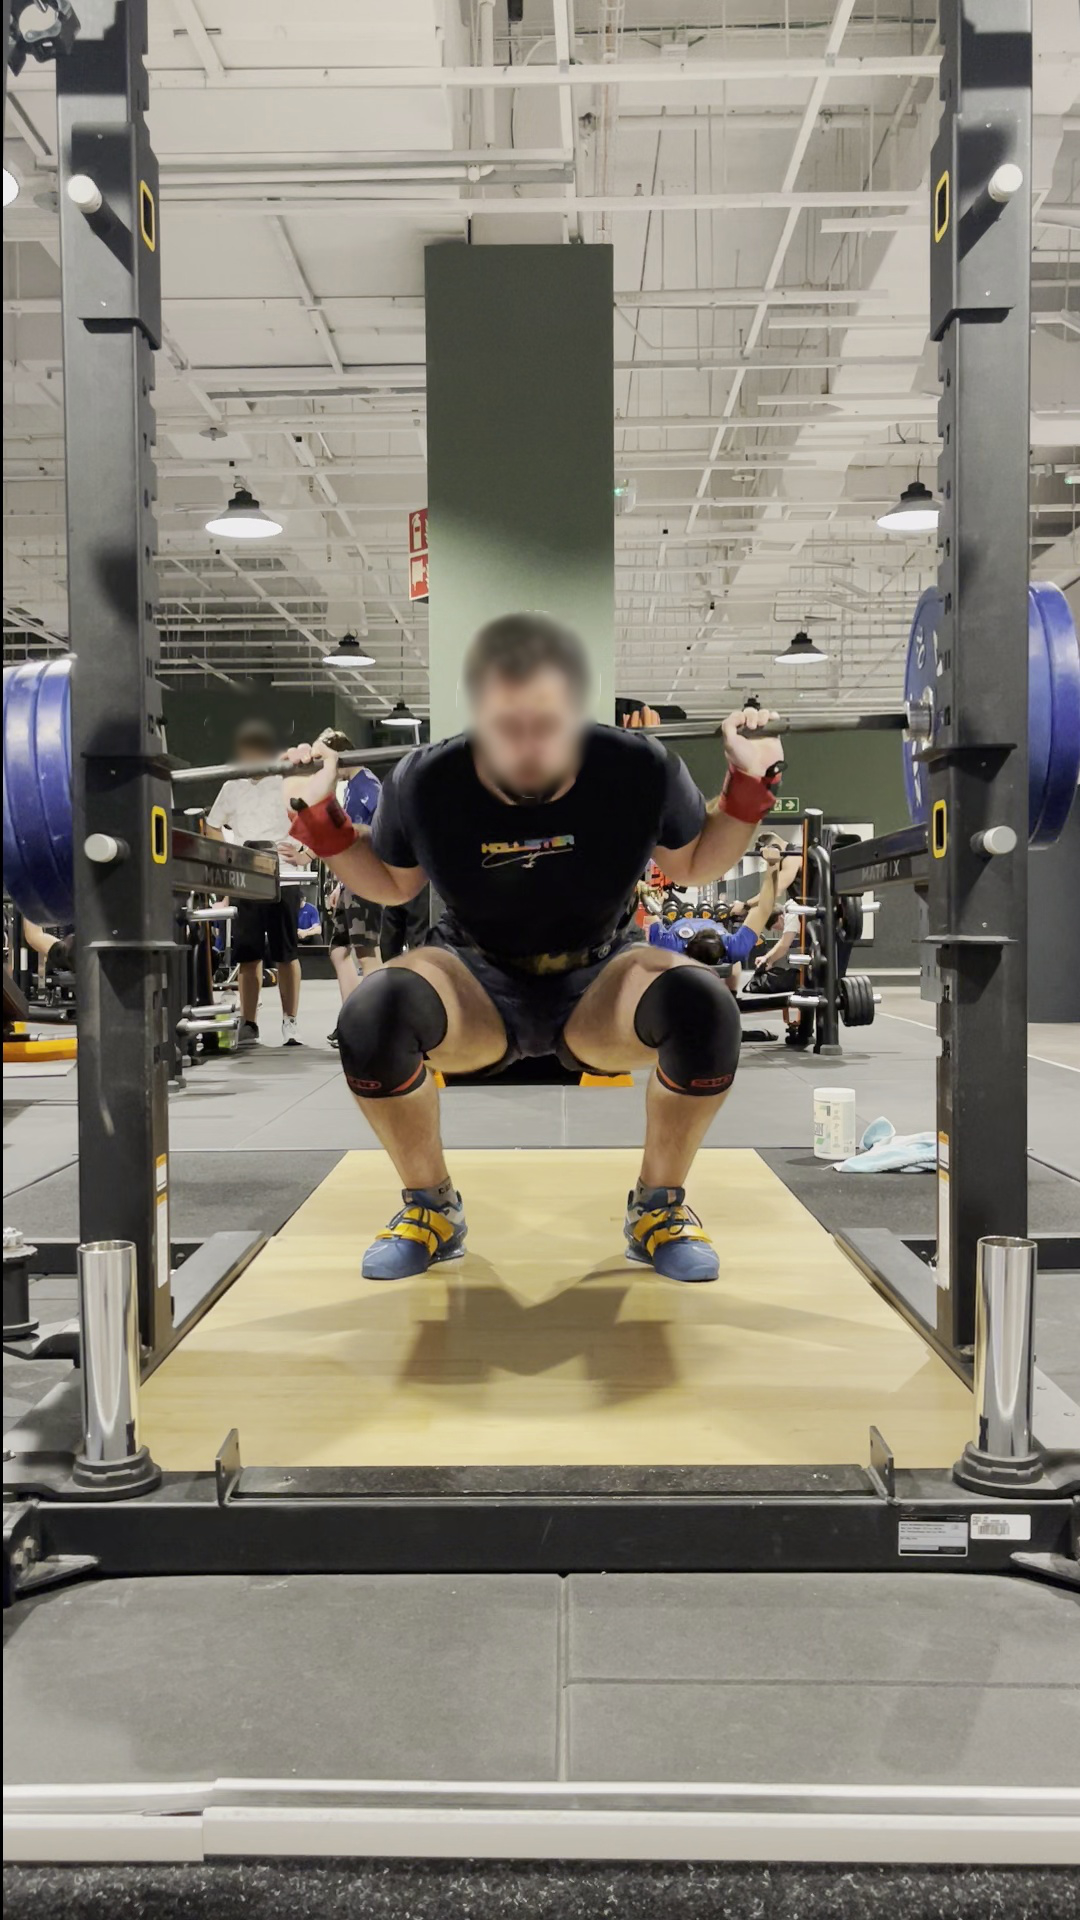
\includegraphics[width=3cm, height=5cm]{images/3-Pipeline_architecture/Background-limitation-frame.jpg}
  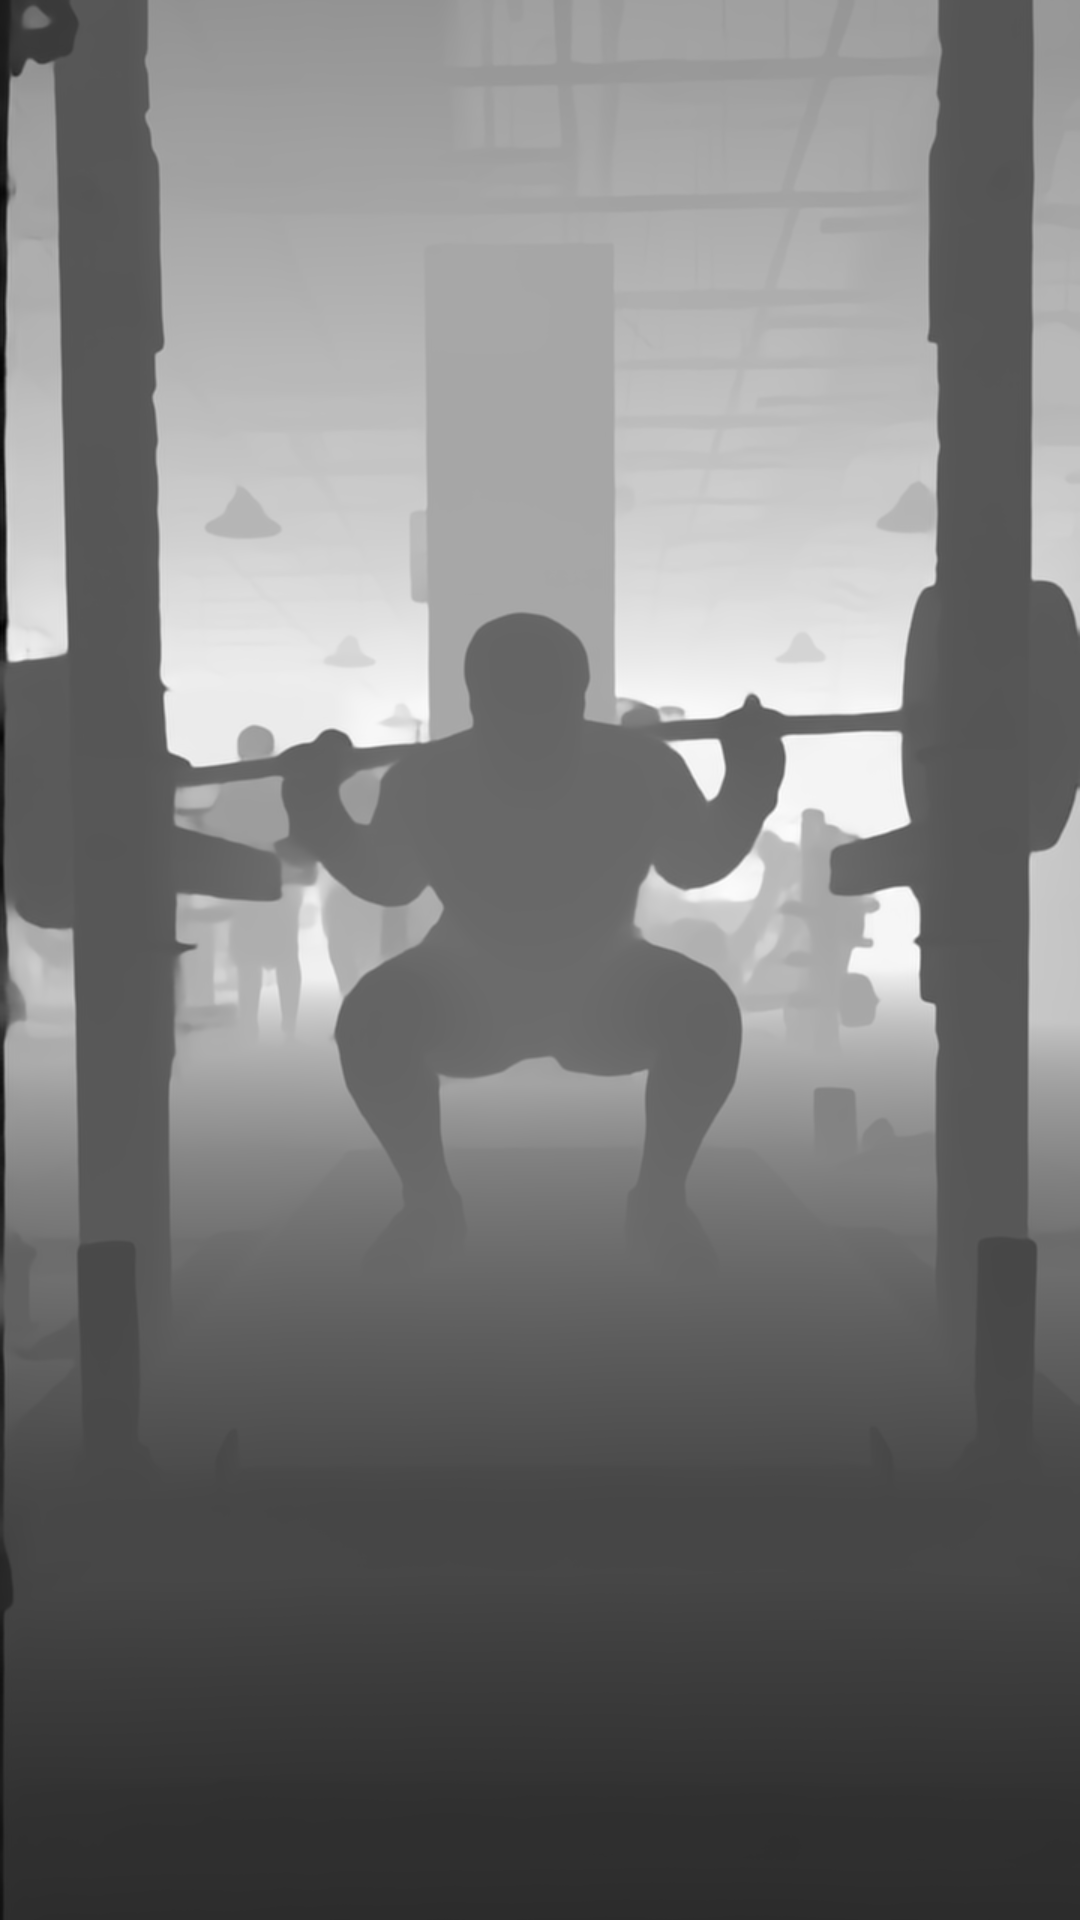
\includegraphics[width=3cm, height=5cm]{images/3-Pipeline_architecture/Background-limitation-moge.png}
  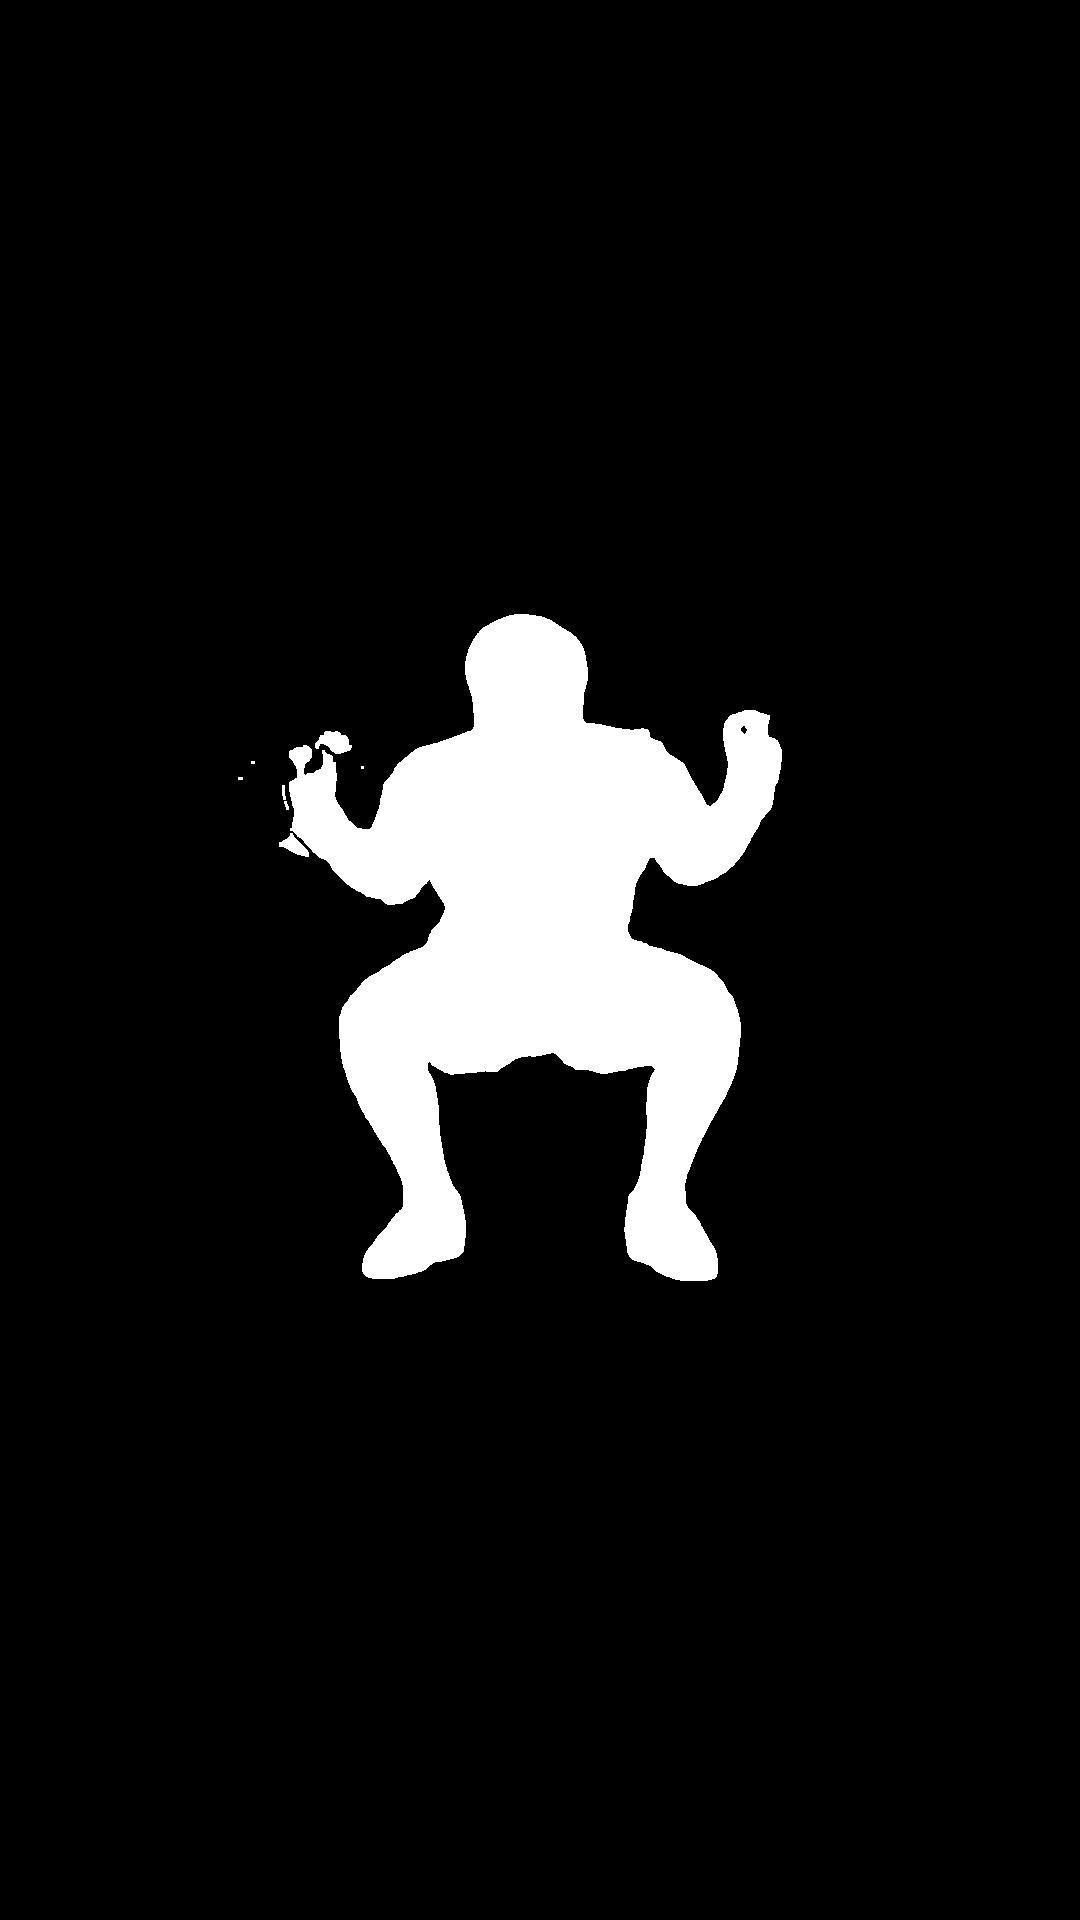
\includegraphics[width=3cm, height=5cm]{images/3-Pipeline_architecture/Background-limitation-mask.png}
  \caption{Confusion entre sujet et fond de couleur similaire}
  \label{fig:background-limitation}
\end{figure}

La principale limite de MoGe-2 dans notre cas est la suivante : la prédiction d'échelle métrique reste sujette à des erreurs de l'ordre de 5 à 10\,\% en environnements très inhabituels~\cite{MoGe2-2025} (très faible éclairage, scènes monochromes, ...), ce qui peut affecter la stabilité du filtre de profondeur.

Une alternative pertinente était UniDepth~\cite{UniDepth-2024}, qui fournit également des prédictions métriques. Il a été écarté en raison d'une qualité de contour inférieure. Depth Anything V2~\cite{Depth-Anything-V2-2024}, malgré son excellente généralisation, a été éliminé pour son absence d'échelle métrique native et sa précison inférieure à MoGe-2~\cite{Depth-Anything-V2-2024}.

\section{Filtre de profondeur et isolation du sujet} \label{sec:filtre-profondeur}

Ces deux étapes intermédiaires, bien que n'utilisant pas de modèle profond, jouent un rôle important dans le pipeline.

\subsection{Filtre de profondeur}

Le filtre de profondeur reçoit en entrée l'ensemble des masques produits par le module 1 (voir section~\ref{sec:module-1}) et la carte de profondeur produite par le module 2 (voir section~\ref{sec:module-2}) pour une trame donnée. Son objectif est d'identifier, parmi tous les masques détectés, celui correspondant au sujet d'intérêt situé au premier plan.

Pour chaque masque, la profondeur médiane des pixels couverts est calculée. Le masque retenu est celui présentant la plus faible profondeur parmi les personnes détectées.

\subsection{Isolation du sujet}

Une fois le masque du sujet identifié, l'isolation consiste simplement à appliquer ce masque sur l'image originale, produisant une séquence d'images où seul le sujet apparaît sur un fond neutre (blanc).

Cette étape remplit deux rôles distincts dans le pipeline. D'une part, elle simplifie radicalement le problème posé aux modules suivants : en supprimant toute personne autre que le sujet d'intérêt, TACO et SAM 3D Body n'ont plus à gérer la présence d'autres pratiquants dans le champ, ce qui évite les confusions d'instance et les reconstructions erronées dues à une silhouette parasite (voir sous-section~\ref{subsec:background-limitation}). D'autre part, elle élimine les biais visuels introduits par l'arrière-plan d'une salle de musculation : miroirs multipliant les instances apparentes du sujet, reflets sur les équipements métalliques, et présence de couleurs similaires à celles de l'habillement de l'athlète dans le fond de la scène (voir sous-section~\ref{subsec:background-limitation}).


\section{Module 3 : Complétion amodale d'occlusions avec TACO} \label{sec:module-3}

\subsection{Principe et architecture}

TACO (\emph{Taming Diffusion for in-the-wild Video Amodal Completion})~\cite{TACO-2025}, publié en 2025, est un modèle de diffusion conditionnel\footnote{Un modèle de diffusion conditionnel est une extension des modèles de diffusion génératifs dans laquelle le processus de débruitage est guidé par un signal de conditionnement externe (image, masque, texte, etc.). Plutôt que de générer des données depuis du bruit pur de manière inconditionnelle, le modèle apprend à produire des sorties cohérentes avec la condition fournie.} dédié à la tâche de \emph{Video Amodal Completion} (VAC). TACO réutilise les variétés \footnote{En apprentissage automatique, une variété (\textit{manifold}) désigne une structure géométrique de basse dimension apprise par le modèle dans l'espace des données. Un modèle de diffusion pré-entraîné apprend implicitement la variété des vidéos naturelles, c'est-à-dire la distribution des apparences et mouvements plausibles.} apprises par un modèle de diffusion vidéo pré-entraîné (\textit{Stable Video Diffusion}, SVD~\cite{SVD-2023}) et les adapte au problème de VAC via un fine-tuning. Le modèle reçoit en entrée une séquence vidéo (\textit{trames}) dans laquelle un objet d'intérêt est partiellement occulté, ainsi que son masque visible. Il produit une séquence vidéo dans laquelle l'objet est entièrement reconstruit, y compris les parties précédemment cachées, avec une cohérence temporelle assurée par la nature vidéo du modèle de diffusion sous-jacent.

L'apprentissage repose sur le dataset synthétique OvO (\emph{Object-video-Overlay})~\cite{TACO-2025}, construit en superposant artificiellement des occlusions synthétiques sur des vidéos non-occultées. Ce dataset est organisé en deux niveaux de difficulté (OvO-Easy et OvO-Hard), et le fine-tuning est conduit progressivement du plus simple au plus complexe.

\subsection{Entrées et sorties dans le pipeline}

Dans le pipeline, TACO reçoit en entrée la séquence d'images isolées ainsi que le masque correspondant au sujet. Sa sortie est une séquence dans laquelle les portions du corps de l'athlète masquées par la barre, les disques ou les structures de sécurité sont reconstruites de façon vraisemblable et temporellement stable.

Ce module est crucial dans le contexte de la force athlétique, lors d'un squat par exemple, les disques ou la structure de sécurité cachent une partie du bras ou de la jambe, et un modèle de reconstruction 3D appliqué directement sur les images occultées produirait des artefacts importants (certaines parties du corps à des positions éronnées).

\subsection{Justification du choix}

Le choix de TACO repose sur trois arguments :

\begin{itemize}
  \item \textbf{Cohérence temporelle.} Contrairement aux méthodes de complétion amodale image par image, TACO exploite explicitement le contexte temporel via le modèle de diffusion vidéo sous-jacent (\textit{Stable Video Diffusion})~\cite{TACO-2025}, évitant le scintillement inter-trames qui dégraderait la reconstruction 3D ultérieure.
  \item \textbf{Capacité en conditions réelles.} TACO a été spécifiquement conçu et évalué pour gérer des vidéos non contraintes, sans hypothèses fortes sur le contexte de capture~\cite{TACO-2025}. Les auteurs rapportent des performances robustes sur des séquences issues d'environnements très variés, ce qui est déterminant dans le contexte d'une salle de musculation.
  \item \textbf{Adaptabilité par fine-tuning.} Le code source de TACO est publié avec des scripts d'entraînement et de fine-tuning directement utilisables~\cite{TACO-2025}. Cette accessibilité ouvre la voie à une spécialisation du modèle sur des données propres au domaine de la force athlétique, comme décrit au chapitre~\ref{ch_four}.
\end{itemize}

\subsection{Limites et alternatives}

TACO présente plusieurs limitations notables. Premièrement, le coût computationnel est élevé, étant basé sur un modèle de diffusion vidéo, il requiert plusieurs secondes d'inférence par séquence sur des GPU haut de gamme, ce qui exclut, ici aussi, tout traitement en temps réel. Deuxièmement, la qualité de la complétion amodale se dégrade lorsque les occlusions couvrent plus de 50\,\% du sujet sur une durée prolongée. Troisièmement, le modèle n'est pas spécialisé sur l'anatomie humaine et peut produire des reconstructions plausibles mais anatomiquement incorrectes (par exemple un coude présentant une flexion irréaliste).

Des alternatives ont été considérées et écartées :
\begin{itemize}
  \item \textbf{pix2gestalt}~\cite{pix2gestalt-2024} effectue une complétion amodale image par image en s'appuyant sur Stable Diffusion. Sans modélisation du contexte temporel, il produit des sorties incohérentes d'une trame à l'autre, ce qui dégrade significativement la qualité de la reconstruction 3D ultérieure.
  \item \textbf{InpaintHuman}~\cite{InpaintHuman-2026} est spécialisé sur l'humain et donc garantit une cohérence anatomique supérieure. Cependant, son intégration nécessite une estimation de pose préalable précise, créant une dépendance circulaire avec le module SAM 3D Body situé en aval de TACO dans le pipeline. Cette contrainte d'ordonnancement a conduit à écarter cette solution.
  \item \textbf{Video inpainting classique}~\cite{ProPainter-2023} atteint d'excellents résultats sur la complétion amodale vidéo, mais ces méthodes requièrent la spécification explicite des masques d'occlusion trame par trame. Or, dans notre cas, identifier automatiquement quelles régions du sujet sont occultées constitue un problème en soi, que TACO résout via la complétion amodale.
  \item \textbf{Diffusion Handles}~\cite{DiffusionHandles-2023} et autres approches de complétion amodale image par image basées sur diffusion souffrent du même défaut que pix2gestalt et ont été écartées pour la même raison.
\end{itemize}


\section{Module 4 : Éstimation de pose avec SAM 3D Body}

\subsection{Principe et architecture}

SAM 3D Body (3DB), publié par Meta en novembre 2025~\cite{SAM-3D-Body-2026}, est un modèle promptable dédié au \emph{Human Mesh Recovery} (HMR)\footnote{\emph{Human Mesh Recovery} désigne la tâche consistant à reconstruire le maillage 3D complet du corps humain (forme corporelle) depuis une ou plusieurs images 2D. Contrairement à l'estimation de pose squelettique qui produit un ensemble discret de keypoints, le HMR produit un maillage dense de plusieurs milliers d'éléments représentant la surface corporelle, incluant la forme du corps (morphologie, corpulence) et la pose (angles articulaires).} à partir d'une image unique. Il atteint l'état de l'art sur plusieurs benchmarks~\cite{SAM-3D-Body-2026} et est conçu pour produire des reconstructions robustes en conditions réelles (\textit{in-the-wild}).

SAM 3D Body repose sur une architecture de type encodeur-décodeur. L'encodeur image adopte une conception multi-entrées capable de capturer des détails à haute résolution pour les parties fines du corps (mains, pieds, visage). Le décodeur prédit les paramètres d'une représentation paramétrique de maillage : la \emph{Momentum Human Rig} (MHR) \footnote{MHR est une représentation paramétrique du corps humain introduite par Meta~\cite{MHR-2025}. Elle encode le corps via deux composantes découplées : un \textit{skeletal rig} définissant la structure articulaire et les rotations osseuses, et une \textit{soft tissue shape} décrivant la forme de la surface cutanée indépendamment de la pose. Ce découplage explicite contraste avec SMPL et SMPL-X, où la forme et la pose sont entremêlées.}. Cette représentation, ouverte et nouvellement introduite par les auteurs, présente la propriété originale de découpler explicitement la structure squelettique (\textit{skeletal rig}) de la forme de la surface (\textit{soft tissue shape}), offrant ainsi une interprétabilité supérieure comparé à SMPL ou SMPL-X.

Le modèle est promptable, il accepte en entrée des masques de segmentation et/ou des keypoints 2D, ce qui permet de guider la reconstruction. Cette propriété n'est pas exploitée dans le pipeline puisque la silhouette sortante de TACO est seule sur un fond uni.

\subsection{Entrées et sorties dans le pipeline}

SAM 3D Body est appliqué trame par trame sur les images produites par TACO. Sa sortie pour chaque trame est un ensemble de paramètres MHR comprenant :
\begin{itemize}
  \item la pose globale du sujet.
  \item les angles articulaires de l'ensemble du squelette, incluant 70 keypoints corps, mains et pieds.
  \item les paramètres de la forme corporelle (\emph{shape parameters}) caractérisant la morphologie du sujet.
\end{itemize}

Ces paramètres permettent de produire un maillage 3D du sujet, qui constitue la sortie finale du pipeline.

\subsection*{Interface de visualisation des résultats}

Une application web de visualisation (figure~\ref{fig:web-visualisation}) a été développée dans le cadre de ce travail de fin d'études pour explorer les reconstructions 3D produites par SAM 3D Body (voir annexe~\ref{ann:web-interface}). Elle permet de naviguer trame par trame dans la séquence reconstruite et affiche en temps réel les métriques biomécaniques calculées à partir des keypoints 3D exportés.

Pour chaque mouvement, des métriques spécifiques aux critères techniques de l'IPF~\cite{IPF-Technical-Regulations-2025} sont calculées à partir des fichiers de keypoints au chargement de la séquence :

\begin{itemize}
  \item \textbf{Squat.} Profondeur de la descente (hanche sous le niveau du genou sur au moins une trame), inclinaison maximale du buste, et asymétrie maximale des hanches sur l'ensemble de la séquence.
  \item \textbf{Développé couché.} Verrouillage des coudes (angle > 160° atteint en fin de mouvement), angle minimal des coudes (profondeur de la descente), et symétrie des poignets.
  \item \textbf{Soulevé de terre.} Verrouillage des genoux, épaules en arrière en position finale, inclinaison maximale du buste, et distance cumulée parcourue par chaque main sur l'ensemble du mouvement.
\end{itemize}

Les métriques globales sont calculées sur l'ensemble de la séquence dès le chargement, tandis que les métriques instantanées (angles courants, symétrie) sont mises à jour à chaque trame. Cette distinction permet à l'entraîneur de distinguer la conformité globale du mouvement de l'état postural à un instant précis.

\begin{figure}[htp]
  \centering
  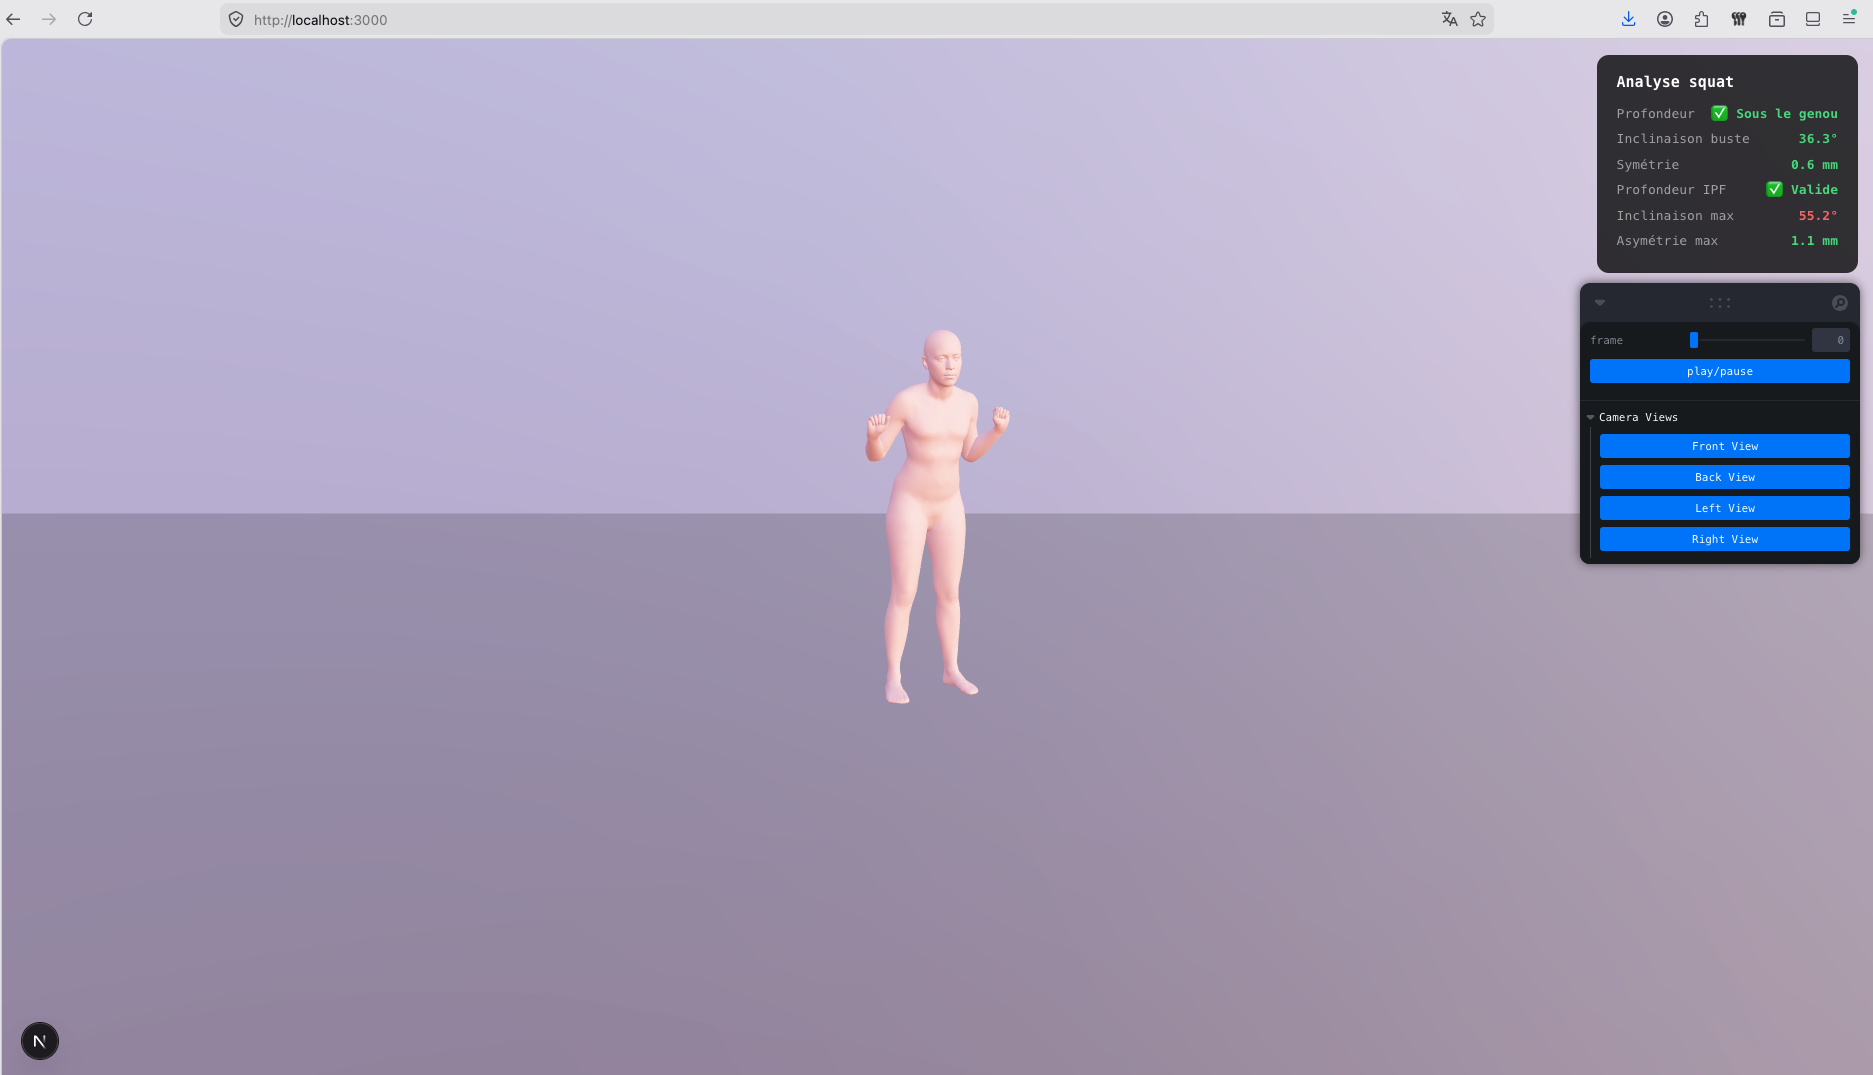
\includegraphics[width=5cm, height=3.5cm]{images/3-Pipeline_architecture/Squat-Web.png}
  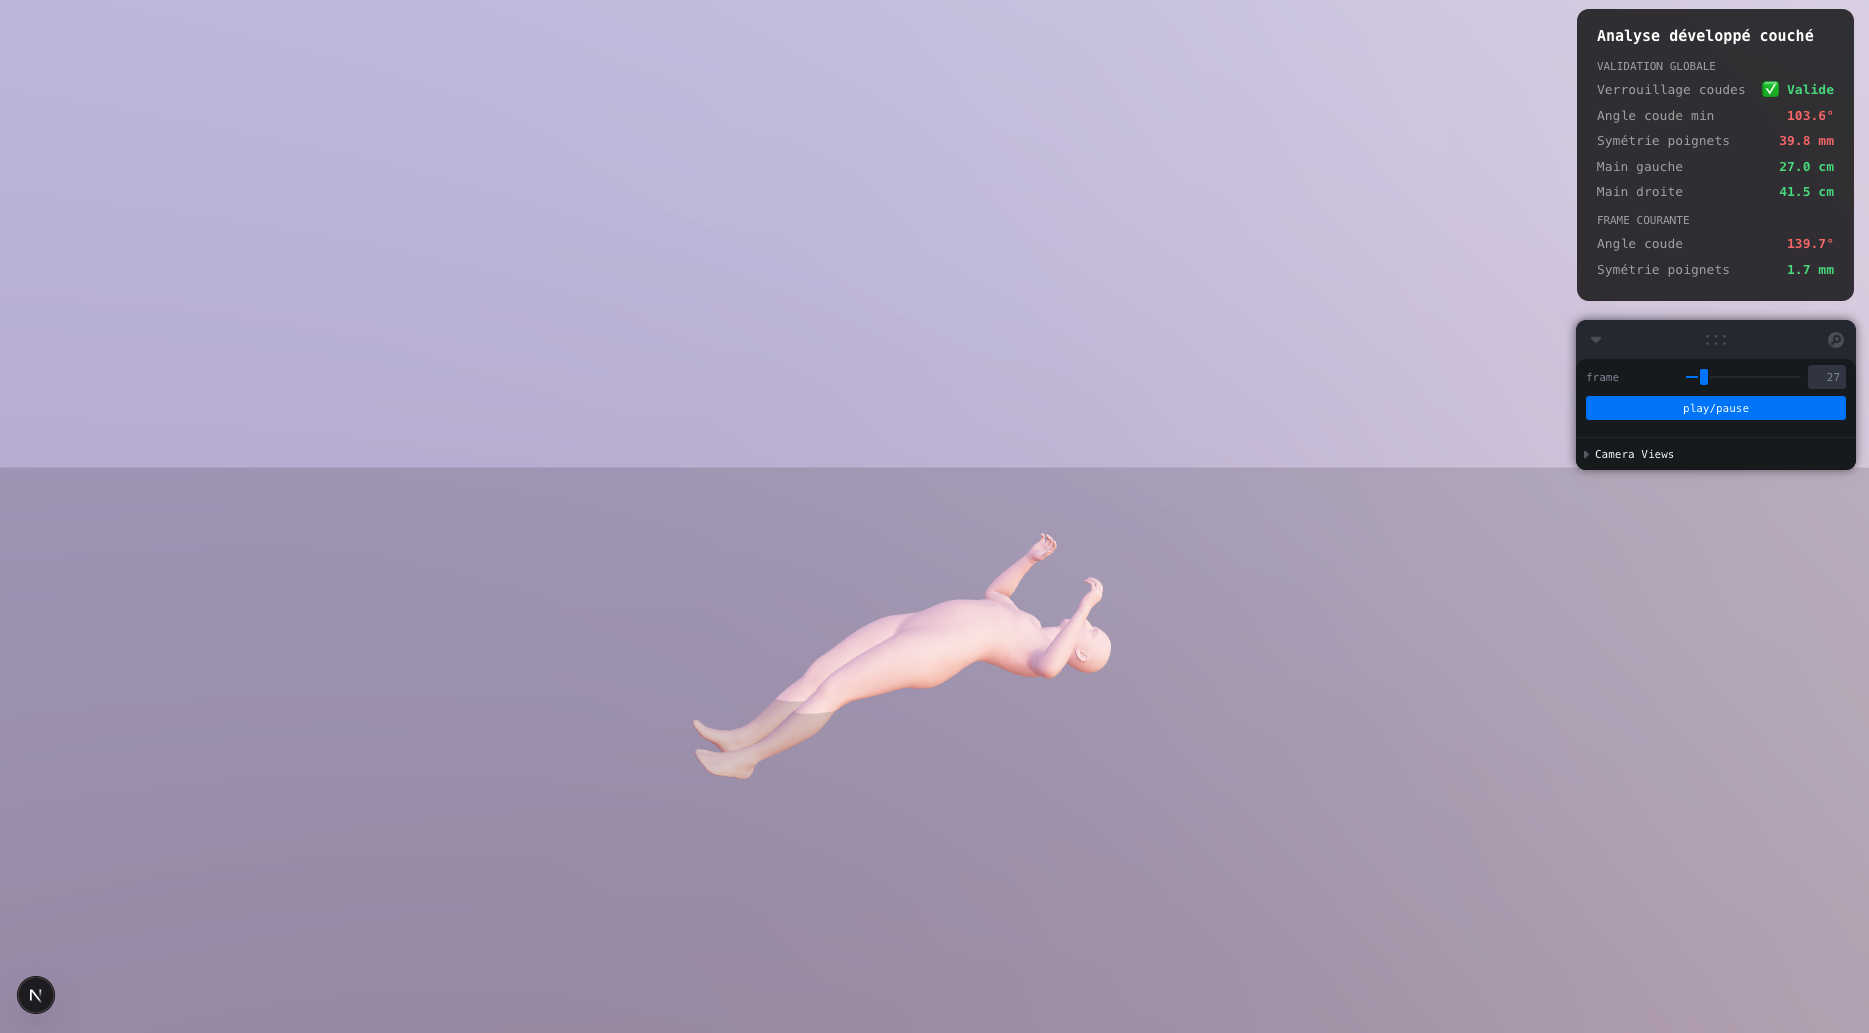
\includegraphics[width=5cm, height=3.5cm]{images/3-Pipeline_architecture/Bench-Web.png}
  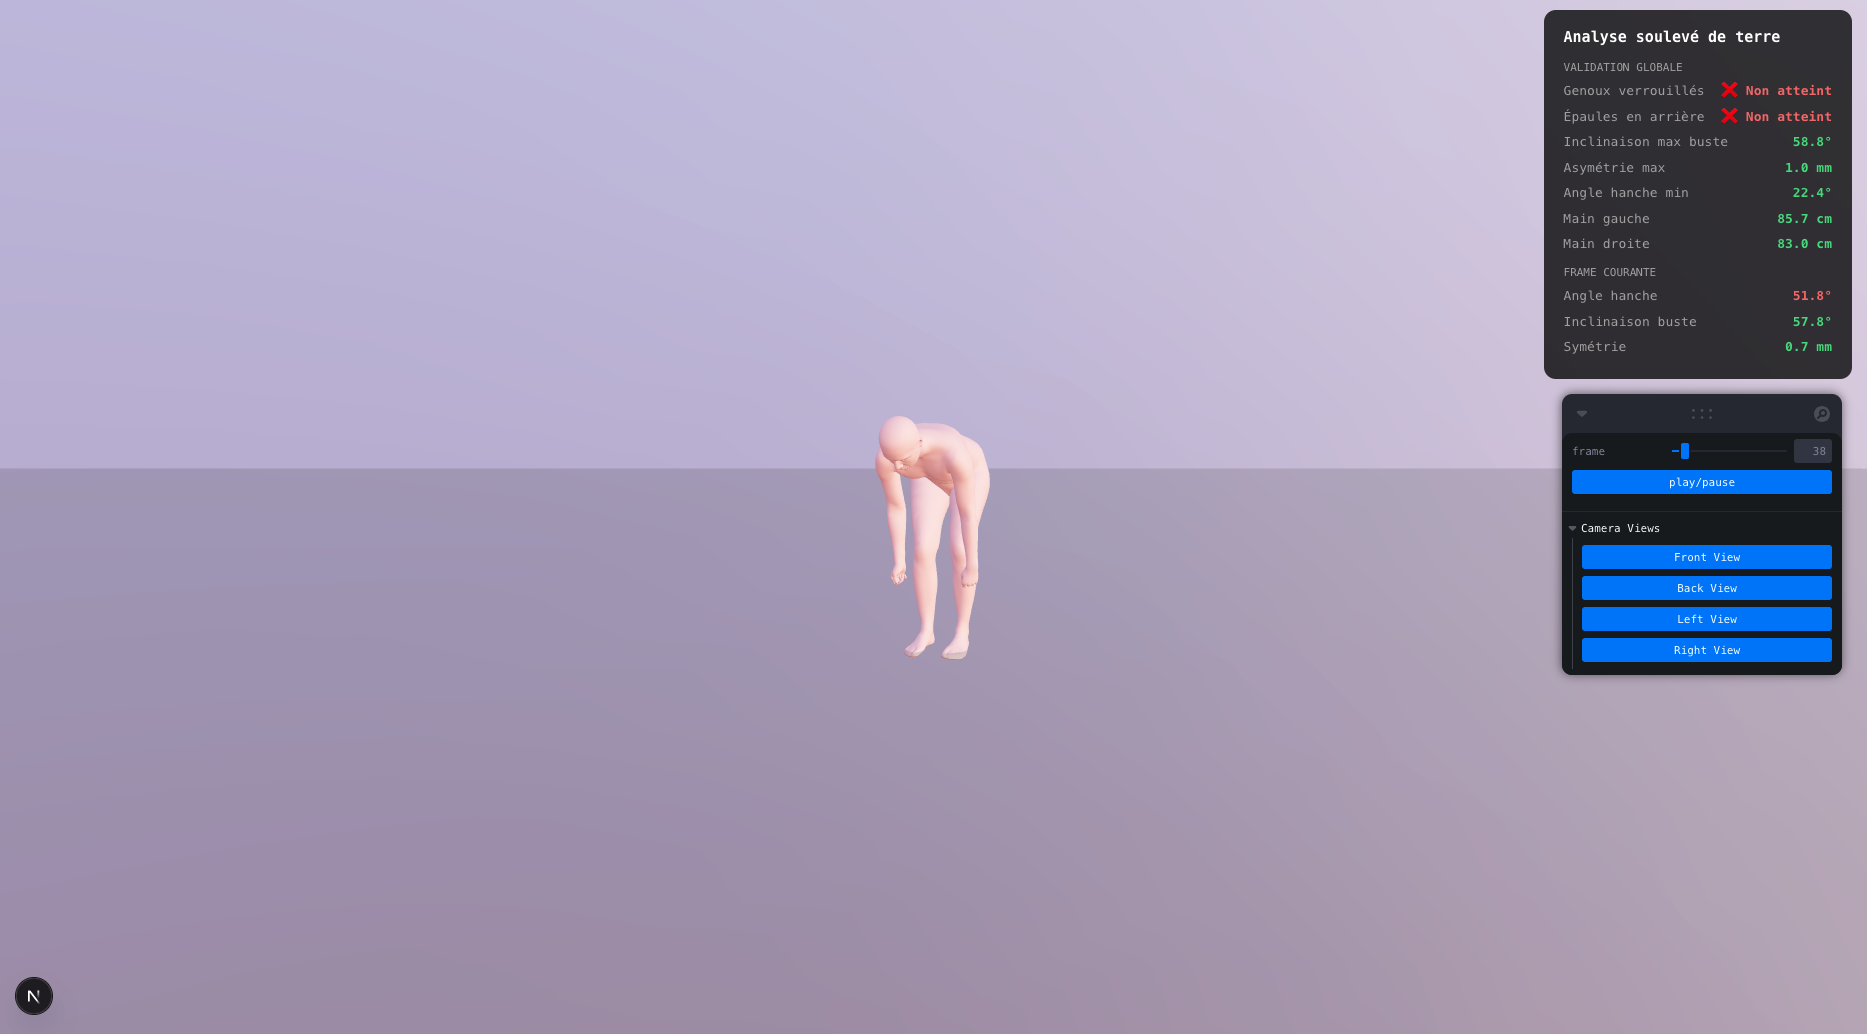
\includegraphics[width=5cm, height=3.5cm]{images/3-Pipeline_architecture/Deadlift-Web.png}
  \caption{Vue d'ensemble de l'application web de visualisation}
  \label{fig:web-visualisation}
\end{figure}

\subsection{Justification du choix}

Le HMR est un domaine compétitif où plusieurs modèles coexistent (PIXIE~\cite{PIXIE-2021}, HybrIK~\cite{HybrIK-2022}, HMR2.0~\cite{HMR-2-2023}, CLIFF~\cite{CLIFF-2022}, SMPLer-X~\cite{SMPLer-X-2024}, OSX~\cite{OSX-2023}, NLF~\cite{NLF-2024}, et SAM 3D Body~\cite{SAM-3D-Body-2026}). Le choix s'est porté sur 3DB pour les raisons suivantes :

\begin{itemize}
  \item \textbf{Performance en conditions réelles.} Les évaluations indépendantes et celles présentées par les auteurs placent 3DB en tête sur les benchmarks de poses inhabituelles et de conditions de prise de vue difficiles~\cite{SAM-3D-Body-2026}, ce qui correspond précisément aux poses extrêmes rencontrées en force athlètique.
  \item \textbf{Reconstruction full-body.} Contrairement à des modèles centrés sur le corps "simple" (SMPL~\cite{SMPL-2015}), 3DB inclut nativement les mains et les pieds, essentiels pour évaluer la prise sur la barre et l'appui au sol.
  \item \textbf{MHR.} Le découplage squelette/surface offert par MHR facilite l'analyse biomécanique : les indicateurs articulaires (angles, vitesses) peuvent être calculés directement sur le squelette sans interférence avec les variations de surface dues à l'habillement par exemple.
  \item \textbf{Open-source.} Le code et les checkpoints sont publiés en open-source, ce qui garantit la reproductibilité et permet un éventuel fine-tuning futur.
\end{itemize}

\subsection{Limites et alternatives}

Une limite principale doit être notée, 3DB opère image par image~\cite{SAM-3D-Body-2026} et ne garantit pas par construction la cohérence temporelle du maillage produit. 

Les alternatives écartées incluent :
\begin{itemize}
  \item HMR2.0 et CLIFF, plus rapides mais limités à SMPL (corps sans mains détaillées).
  \item SMPLer-X, corps entier mais moins robuste sur les poses extrêmes.
\end{itemize}

\section{Intégration et synchronisation des modules} \label{sec:integration}

\subsection{Gestion des dépendances et environnements}

Chaque modèle a été développé indépendamment par des équipes différentes, avec des dépendances Python parfois incompatibles (versions de PyTorch, CUDA, transformers, diffusers). Pour résoudre ce conflit, Pixi~\cite{Pixi-2024} a été utilisé comme gestionnaire d'environnements. Cet outil permet de créer un environnement isolé pour chaque module et de définir des pipelines d'exécution automatisant certaines tâches fastidieuses, notamment la construction du dataset.

\subsection{Synchronisation temporelle}

Les modules SAM3, MoGe-2 et SAM 3D Body opèrent trame par trame, produisant une sortie indépendante pour chaque image de la séquence. TACO, en revanche, requiert en entrée un clip vidéo de longueur fixe (14 trames consécutives dans la configuration retenue) et produit une séquence reconstruite de même longueur.

Pour traiter des séquences vidéo de longueur arbitraire avec TACO, une stratégie de fenêtre glissante sans chevauchement est appliquée : la séquence est découpée en clips de 14 trames consécutives et non recouvrantes. Lorsque la longueur totale de la séquence n'est pas un multiple de 14, la dernière fenêtre est décalée vers la gauche pour inclure les trames finales, créant un recouvrement minimal avec l'avant-dernière fenêtre. Les trames déjà reconstruites par la fenêtre précédente ne sont pas réécrites.

L'approche idéale consisterait à traiter la séquence entière en une seule passe, en fournissant à TACO l'intégralité des trames comme contexte temporel. Cela permettrait au modèle de tirer parti de la cohérence globale du mouvement pour guider la reconstruction des régions occluses. Cette approche se heurte toutefois aux limitations actuelles de la mémoire GPU : charger une séquence complète de plusieurs centaines de trames en mémoire vidéo reste hors de portée du matériel disponible. Le traitement par fenêtres de 14 trames constitue donc un compromis pratique, au prix d'une perte de contexte entre les fenêtres consécutives. Cette limite est identifiée comme une piste d'amélioration dans le chapitre~\ref{ch_six}.

\section{Choix techniques et justifications}

Au-delà du choix individuel des modèles, plusieurs décisions architecturales méritent d'être explicitées et sont détaillées dans cette section.

\subsection{Architecture séquentielle vs. bout-en-bout}

Une alternative aurait consisté à entraîner un unique modèle bout-en-bout, prenant en entrée une vidéo brute et produisant directement un maillage 3D animé. Cette approche a été écartée pour plusieurs raisons :

\begin{itemize}
  \item \textbf{Données d'entraînement.} Aucun dataset public ne fournit conjointement les annotations nécessaires (segmentation, profondeur métrique, complétion amodale, maillage 3D full-body) à l'échelle requise pour entraîner un tel système.
  \item \textbf{Coût.} L'entraînement d'un modèle multi-tâches de cette ampleur dépasserait largement les ressources et le temps disponibles dans le cadre de ce mémoire.
  \item \textbf{Modularité.} La rapide évolution de l'état de l'art rend hautement souhaitable la possibilité de remplacer un module sans réentraîner l'ensemble. Entre la planification du pipeline et sa finalisation, un des quatre modèles utilisés a reçu une mise à jour majeure (SAM3 $\to$ SAM 3.1~\cite{SAM3.1-2026}), introduisant une approche à mémoire partagée pour le suivi multi-objets, significativement plus rapide sans perte de précision.
\end{itemize}

\subsection{Inférence sur GPU} \label{sec:inference-sur-GPU}

L'ensemble du pipeline est conçu pour s'exécuter sur deux GPU NVIDIA RTX A5000. Cette contrainte a imposé un séquencement strict des modules avec libération de la mémoire GPU entre chaque étape.

\subsection{Choix du langage et du tramework}

L'ensemble du pipeline est implémenté en Python. Ce choix s'impose naturellement car tous les modèles sélectionnés étant distribués sous ce language. L'orchestration inter-modules est gérée par des scripts en Python pur.

\subsection{Versionnage des modèles et reproductibilité}

Chaque module est associé à un checkpoint figé, identifié par son empreinte cryptographique SHA-256. Les versions exactes utilisées dans ce mémoire sont consignées dans un fichier \texttt{models.lock} versionné avec le code source, garantissant la reproductibilité des résultats malgré les mises à jour fréquentes des modèles en amont. Les checkpoints eux-mêmes sont hébergés séparément et accessibles via les liens fournis dans le dossier \texttt{code/checkpoints} du dépôt.

Chaque module est associé à un checkpoint figé. Les versions exactes utilisées dans le mémoire sont consignées dans un fichier \texttt{models.lock} versionné avec le code source, garantissant la reproductibilité des résultats malgré les mises à jour fréquentes des modèles.

\medskip
Le pipeline défini ci-dessus constitue la base technique de la contribution principale de ce mémoire. Le chapitre suivant détaille la construction d'un dataset spécialisé et le protocole de \emph{fine-tuning} de TACO mis en place.
% ---------------------
% DATASET ET FINE-TUNING DU MODELE DE DIFFUSION
% ---------------------
\chapter{Dataset et fine-tuning du modèle de diffusion} \label{ch_four}

\section{Justification du fine-tuning}

Les modèles SAM3, MoGe-2 et SAM 3D Body relèvent des architectures fondationnelles. Leur entraînement à très grande échelle leur permet une généralisation robuste ainsi qu'une spécialisation à la tâche de type \textit{zero-shot}, mais implique des contraintes en termes de ressources (voir section~\ref{sec:inference-sur-GPU}). À l'inverse, le modèle de complétion amodale vidéo par diffusion TACO dépend strictement de ses données d'apprentissage et il est mono-tache, il ne peut pas être utilisé directement pour la complétion amodale de sujets humains dans des vidéos de force athlétique sans adaptation préalable.

L'architecture TACO a été entraînée sur un dataset synthétique composé d'environ 200\,000 paires de vidéos~\cite{TACO-2025}, élaboré en superposant des occlusions artificielles sur des séquences sources préalablement identifiées comme non-occultées. Bien que cette méthode d'entraînement permette une adaptation sur des bases de données généralistes, son transfert direct vers l'analyse de la force athlétique expose certains problèmes :

\begin{itemize}
  \item \textbf{Manque d'occlusions spécifiques.} Le dataset OvO utilisé pour entraîner TACO~\cite{TACO-2025} est construit à partir de cinq sources génériques (MVImgNet, SA-V, BDD100K, SA-1B, Objaverse), couvrant des objets du quotidien, des scènes de conduite et des environnements intérieurs. Aucune de ces sources ne contient de séquences de force athlétique, et les auteurs ne décrivent aucune procédure de filtrage orientée vers ce domaine. La probabilité que des occlusions par des disques de fonte ou des racks à squat figurent dans le dataset d'entraînement est donc négligeable, ce qui justifie l'adaptation par fine-tuning.
  \item \textbf{Cadrages et perspectives atypiques.} Les vidéos issues d'environnements ouverts n'ont pas les mêmes angles de capture imposés par les standards d'évaluation de force athlétique (cadrage serré, prise de vue rasante).
\end{itemize}

L'incapacité des datasets publics à reproduire l'environnement de la force athlétique invalide l'usage direct du modèle. La création d'un dataset propriétaire, incluant les masques et les occlusions synthétiques spécifiques, ainsi qu'un \textit{fine-tuning} de TACO, constituent un prérequis pour garantir une restauration amodale correcte.

\section{Collecte et critères de sélection des vidéos}

Compte tenu de l'absence de dataset public adapté, une stratégie de collecte ciblée a été privilégiée à l'accumulation massive. Le dataset constitué comprend moins de 100 séquences vidéo (voir annexe~\ref{ann:dataset-details}), ce qui se justifie par l'adoption d'une stratégie de fine-tuning par adaptation à faible rang (LoRA, voir section~\ref{sec:protocole}) qui ne nécessite que peu de données pour spécialiser un modèle pré-entraîné.

\subsection{Sources de collecte}

Les vidéos sources ont été récoltées depuis deux canaux différents :

\begin{itemize}
  \item \textbf{Captations propres.} Une partie du dataset provient de sessions d'entraînement filmées par l'auteur de ce travail de fin d'études, dans des conditions contrôlées où le cadrage et le positionnement du matériel étaient maîtrisés (sujet seul dans le champ, équipement obstructif écarté lorsque l'exercice le permet).

  \item \textbf{Captations auprès de pratiquants volontaires.} La majorité du dataset provient de séquences filmées par des pratiquants de force athlétique sollicités spécifiquement pour ce mémoire. Chaque participant a filmé ses propres sessions d'entraînement selon certains paramètres fournis (cadrage, angle de prise de vue, conditions de captation).
\end{itemize}

Le recrutement de ces volontaires s'est avéré particulièrement long et restrictif, la communauté des pratiquants de force athlétique filmant leurs entraînements dans des conditions exploitables (caméra fixe, cadrage complet, qualité suffisante) reste limitée, et l'établissement tardif de la charte RGPD (voir annexe~\ref{ann:rgpd}) du projet (détaillant le consentement éclairé, la finalité de traitement, et les modalités de retrait) a réduit le temps disponible pour la collecte. Ce facteur explique en grande partie la taille restreinte du dataset constitué.

\subsection{Critères de sélection}

Les séquences retenues satisfont conjointement les critères suivants :

\begin{enumerate}
  \item \textbf{Visibilité intégrale du sujet.} L'athlète apparaît dans son entièreté dans le champ de vision (tête, tronc, membres supérieurs et inférieurs visibles), condition nécessaire pour disposer d'une référence non-occluse exploitable.
  \item \textbf{Absence d'occlusions au moment de la capture source.} La séquence ne contient pas d'éléments d'équipement masquant le sujet. Les occlusions seront ajoutées synthétiquement dans une seconde étape.
  \item \textbf{Stabilité du cadrage.} La caméra reste fixe ou présente des mouvements lents et continus, conformément à la pratique standard d'évaluation en force ahlétique.
  \item \textbf{Qualité visuelle suffisante.} Résolution minimale de 360p, fréquence de capture d'au moins 25 images par seconde, exposition correcte du sujet.
  \item \textbf{Diversité morphologique et vestimentaire.} Sélection veillant à représenter différents gabarits, sexes, tenues d'entraînement et types d'éclairage afin d'éviter un biais de spécialisation excessif.
  \item \textbf{Diversité des exercices.} Les trois mouvements de référence de la force athlétique sont représentés : squat, développé couché, soulevé de terre.
\end{enumerate}

\subsection{Axes de généralisation visés}

La constitution du dataset est guidée par cinq axes de variabilité selon lesquels le modèle fine-tuné doit généraliser, indépendamment du mouvement effectué :

\begin{itemize}
  \item \textbf{Variabilité inter-individu.} Morphologies, sexes et gabarits différents afin que le modèle ne mémorise pas une silhouette corporelle particulière.
  \item \textbf{Variabilité inter-éclairage.} Conditions lumineuses variées (éclairage artificiel de salle, lumière naturelle, contre-jour partiel) pour éviter une dépendance aux niveaux de luminosité ou aux températures de couleur spécifiques à un lieu.
  \item \textbf{Variabilité inter-salle.} Arrière-plans, textures de sol et configurations de salle différentes, afin que le modèle ne s'appuie pas sur des indices contextuels fixes pour la reconstruction.
  \item \textbf{Variabilité inter-caméra.} Résolutions, angles de capture et distances focales variées, reflétant la diversité des dispositifs utilisés par les pratiquants (smartphone, caméra, lentilles).
  \item \textbf{Variabilité inter-angle de prise de vue.} Les vidéos doivent être filmées depuis des angles variés (face, trois-quarts, profil) afin que le modèle ne soit pas biaisé vers une configuration de capture particulière. En compétition officielle, les caméras sont généralement positionnées de côté ou en trois-quarts, tandis que les entraînements sont fréquemment filmés de face. Couvrir ces différentes perspectives garantit une robustesse de la complétion amodale indépendamment de l'angle depuis lequel l'occlusion est observée.
  \item \textbf{Variabilité inter-matériel.} Disques, racks et bancs de marques et coloris différents, afin que la reconnaissance des occlusions synthétiques ne soit pas conditionnée à un équipement spécifique.
  \item \textbf{Variabilité inter-tenue.} Vêtements d'entraînement variés (couleurs, coupes, équipements de compétition tels que \textit{singlets} et genouillères) pour que la reconstruction de la silhouette soit robuste à la texture vestimentaire.
  \item \textbf{Variabilité du taux d'occlusion.} La surface du sujet masquée par l'occlusion varie selon le chargement de la barre (barre vide vs barre chargée avec plusieurs disques superposés), la phase du mouvement et l'angle de capture. Le dataset doit couvrir un spectre allant des occlusions partielles (un seul disque masquant une épaule) aux occlusions massives (barre chargée masquant intégralement le torse), afin que le modèle ne soit pas biaisé vers un taux d'occlusion particulier. Cette variabilité est partiellement contrôlée par la contrainte de couverture maximale de 60\,\% imposée lors de la génération synthétique des occlusions (voir section~\ref{sec:protocole}).
\end{itemize}

Ces axes de généralisation conditionnent directement la constitution des partitions du dataset. Idéalement, chaque partition devrait couvrir l'ensemble de ces axes de façon équilibrée, de sorte que la validation et le test mesurent effectivement la capacité de généralisation et non la mémorisation. En pratique, la taille restreinte du dataset (moins de 100 séquences) ne permet pas une couverture exhaustive et équilibrée de toutes les combinaisons. La partition est donc réalisée en veillant à ce qu'aucun individu, aucune salle et aucune configuration de matériel présents dans les données de tests ne figurent dans les données d'entraînements, minimisant ainsi le risque de surapprentissage sur les exemples vus.

\section{Stratégie d'annotation et construction des paires}

La construction du dataset de fine-tuning suit une procédure entièrement automatisée illustrée à la figure~\ref{fig:pipeline-finetuning}, qui réutilise les premiers modules du pipeline d'inférence décrits au chapitre~\ref{ch_three}. Cette réutilisation présente un avantage, les données d'entraînement présentent exactement la même distribution de prétraitement (segmentation, isolation du fond) que celles qui seront effectivement présentées au modèle en production, éliminant tout écart de domaine entre entraînement et inférence.

\begin{figure}
  [htp]
  \centering
  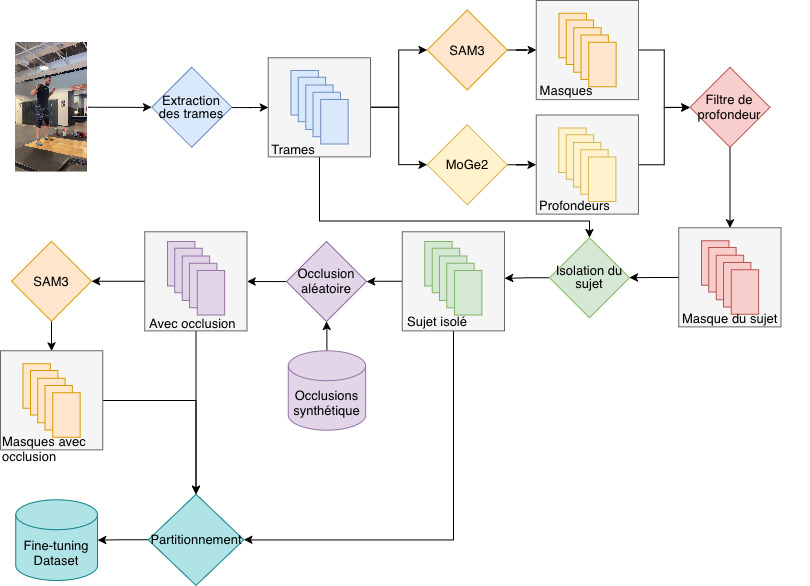
\includegraphics[height=9.5cm]{images/4-Dataset_and_fine-tuning/Dataset-Pipeline.jpg}
  \caption{Pipeline de construction du dataset de fine-tuning}
  \label{fig:pipeline-finetuning}
\end{figure}

\subsection{Extraction du sujet sur fond neutre}

Chaque séquence vidéo brute est d'abord traitée par les modules SAM3 et MoGe-2, suivis du filtre de profondeur. La sortie est l'ensemble des \emph{masques du sujet au premier plan} pour chaque trame de la séquence, identifiant l'athlète isolé du reste de la scène. Une étape de vérification manuelle est conduite trame par trame sur cette sortie. Cette vérification est essentielle sur un dataset de petite taille, chaque erreur d'annotation pèse proportionnellement plus lourd sur l'apprentissage.

L'étape suivante, dite d'\emph{isolation du sujet}, applique ce masque sur les images originales pour produire une séquence où seul l'athlète apparaît, le fond étant remplacé par du blanc uniforme. Ces images isolées constituent la cible (\emph{ground truth}) du fine-tuning, elles représentent la sortie idéale que le modèle TACO devrait produire face à des données occluses.

\subsection{Génération synthétique des éléments occultants}

À partir des images isolées, des occlusions synthétiques (figure~\ref{fig:occlusion-synthétique}) sont superposées aléatoirement. La stratégie reprend la méthodologie OvO (\emph{Object-video-Overlay}) introduite par les auteurs de TACO~\cite{TACO-2025}, mais avec une banque d'occlusions synthétiques spécialisée pour la force athlétique :

\begin{itemize}
  \item \textbf{Disques de fonte calibrés.} Banque d'images de disques de compétition provenant du catalogue produit du distributeur Rogue Fitness~\cite{Rogue-Fitness-Plates}, extraits sur fond transparent depuis des photographies à haute résolution. Les disques respectent le code couleur normalisé par l'IPF \footnote{L'\textit{International Powerlifting Federation} (IPF) impose un code couleur strict pour les disques de compétition~\cite{IPF-Technical-Regulations-2025} : rouge pour 25\,kg, bleu pour 20\,kg, jaune pour 15\,kg, vert pour 10\,kg et blanc pour 5\,kg. Ce code couleur universel garantit l'identification rapide des charges par les juges et les athlètes lors des compétitions officielles.} (5, 10, 15, 20 et 25\,kg). Des images de disques provenant de salles commerciales, dont les couleurs peuvent différer des standards IPF, ont également été intégrées à la banque afin d'améliorer la diversité visuelle. Un retournement horizontal (\textit{flip}) a été appliqué à chaque occlusion pour doubler la diversité des configurations. Des configurations à disques multiples ont également été générées en superposant plusieurs disques de diamètres différents, reproduisant l'apparence d'une barre chargée à l'entrainement où plusieurs disques sont empilés de part et d'autre de l'axe.
  \item \textbf{Racks à squat.} Banque d'images de structures verticales et horizontales (montants de rack et sécurités) également extraites sur fond transparent. Ces éléments reproduisent l'obstruction caractéristique observée lors des squats où les montants du rack masquent partiellement le torse ou les jambes du sujet.
\end{itemize}

Pour chaque clip isolé, une occlusion est sélectionnée aléatoirement dans la banque. Pour chaque occlusion, une position aléatoire est calculée permettant à l'occlusion de masquer une partie visible du sujet.


\begin{figure}
  [htp]
  \centering
  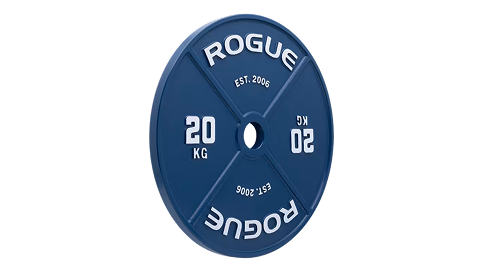
\includegraphics[width=4.5cm, height=2.5cm]{images/4-Dataset_and_fine-tuning/object_13_plate.png}
  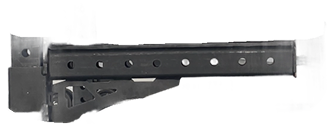
\includegraphics[width=4.5cm, height=2.5cm]{images/4-Dataset_and_fine-tuning/object_10_rack.png}
  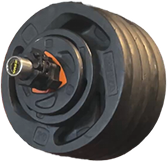
\includegraphics[width=2.5cm, height=2.5cm]{images/4-Dataset_and_fine-tuning/object_3_plate.png}
  \caption{Illustration de 3 exemples d'occlusions synthétiques}
  \label{fig:occlusion-synthétique}
\end{figure}

\subsection{Recalcul du masque visible}

Une fois la version occluse obtenue, une seconde passe de SAM3 est effectuée sur ces images pour produire le \emph{masque du sujet avec occlusion}, c'est-à-dire le masque ne couvrant que les portions visibles du sujet après superposition. Ce recalcul par SAM3 est préféré à un simple calcul de différence pour deux raisons :

\begin{itemize}
  \item \textbf{Robustesse aux occlusions synthétiques à contours flous.} Les bords d'un disque avec une transparence partielle ne sont pas binaires, SAM3 produit un masque visible cohérent avec ce qui est effectivement perçu, là où une différence produirait des contours aberrants.
  \item \textbf{Cohérence avec le pipeline d'inférence.} En réalité, le masque visible du sujet sera effectivement calculé par SAM3 sur les images occluses. Reproduire cette même procédure lors de la construction du dataset garantit que TACO est entraîné dans les mêmes conditions qu'il sera utilisé.
\end{itemize}

Le triplet (\texttt{occluded\_frame}, \texttt{visible\_mask}, \texttt{amodal\_object}) constitue un échantillon d'entraînement : les deux premiers éléments forment l'entrée fournie au modèle (la trame occluse à reconstruire et le masque indiquant les régions visibles du sujet), le troisième la cible (le sujet isolé non occlus servant de vérité terrain).

Le dataset complet est partitionné en sous-ensembles d'entraînement (70\,\%, 17 vidéos sources, 136 séquences) et de validation (30\,\%, 6 vidéos sources, 48 séquences) selon un découpage aléatoire par vidéo source (graine fixée à 42), garantissant que toutes les augmentations dérivées d'une même vidéo source (\textit{original}, \textit{blur}, \textit{contrast}, \textit{flipped}, etc.) sont systématiquement assignées à la même partition. Ce choix prévient toute fuite de données liée à la présence simultanée de variantes quasi-identiques en entraînement et en évaluation.

Cependant, le découpage étant réalisé par vidéo et non par sujet, quatre sujets apparaissent simultanément dans les partitions d'entraînement et de validation. Cette situation représente une limite méthodologique car la validation mesure partiellement la capacité du modèle à généraliser à de nouveaux individus et sa capacité à généraliser à de nouvelles sessions d'un même individu. Un découpage strict par sujet aurait été préférable mais n'était pas réalisable compte tenu du nombre limité de sujets distincts disponibles dans le dataset.

\subsection{Adaptation des dimensions au format d'entrée du modèle}

Les trames extraites des vidéos sources sont initialement de dimensions variables (typiquement 1920$\times$1080 ou 1280$\times$720 selon les vidéos). Le modèle TACO requiert des entrées au format $384 \times 384$, correspondant à la résolution native d'entraînement du checkpoint et au compromis le plus stable en mémoire sur la configuration matérielle disponible (2$\times$RTX A5000 de 24 Go).

Le chargeur de données (\textit{dataloader}) natif de TACO (\texttt{VACDataset}) applique un redimensionnement direct vers $384 \times 384$ au chargement de chaque trame, sans préservation du ratio d'aspect. Cette stratégie, choisie par les auteurs du modèle pour homogénéiser le format d'entrée, introduit une déformation du sujet, une trame $16:9$ source se voit comprimée verticalement (ou étirée horizontalement) pour s'inscrire dans un format carré.

Deux conséquences méthodologiques en découlent :

\begin{itemize}
  \item \textbf{Cohérence entrainement/inférence.} L'entraînement et l'inférence appliquent la même déformation, donc le modèle apprend à reconstruire des silhouettes anatomiquement déformées mais cohérentes avec ce qui sera présenté en production. Tant que le pipeline finale applique le même prétraitement, les proportions seront restituées correctement à la sortie.
  \item \textbf{Anatomie apprise déformée.} Le modèle apprend des proportions corporelles distordues par le ratio. Pour une utilisation impliquant des mesures biomécaniques précises (angles articulaires), il sera nécessaire d'appliquer une transformation inverse en post-traitement ou d'envisager un crop préalable préservant le ratio. Il a été choisi de faire une transformation inverse en post-traitement pour récupérer les proportions anatomiques de départ, afin de ne pas introduire de nouveaux artefacts liés à un recadrage (perte d'information sur les extrémités, variations de cadrage entre les vidéos sources) et pour conserver la simplicité du pipeline d'entraînement.
\end{itemize}

\section{Augmentation et équilibrage du dataset}

Pour pallier la taille restreinte du dataset (moins de 100 séquences), des stratégies d'augmentation de données ont été utilisées.

\subsection{Augmentation par variation des occlusions synthétiques}

Une banque d'occlusions synthétiques a été constituée, regroupant deux catégories distinctes :
\begin{itemize}
  \item \textbf{Disques} : configurations variant selon le nombre de disques superposés sur la barre et leur couleur, correspondant aux différents poids selon les standards IPF (5, 10, 15, 20, 25\,kg), chaque couleur étant associée à un calibre spécifique.
  \item \textbf{Racks} : structures de support fixes utilisées comme sécurité lors du mouvement de squat.
\end{itemize}

Pour chaque clip d'entraînement, une occlusion unique est tirée aléatoirement dans la banque et conservée pendant toute la durée de la séquence, afin de simuler une occlusion temporellement cohérente. Le comportement spatial de l'occlusion dépend de sa catégorie. Les racks sont positionnés à un emplacement fixe à proximité du sujet, reproduisant le caractère statique de ce type d'élément dans la scène réelle. Les disques suivent une trajectoire verticale montante ou descendante au fil des trames, leur position horizontale restant constante. Le déplacement du disque reproduisant la dynamique d'une barre en mouvement durant un mouvement.

La position initiale, le calibre et l'amplitude de la trajectoire sont rééchantillonnés à chaque itération, sous la contrainte que la couverture de la silhouette n'excède jamais 60\,\% sur les trames du clip. Cette stratégie multiplie considérablement la diversité des configurations vues par le modèle, combinée aux 8 augmentations visuelles par vidéo source et à l'échantillonnage temporel aléatoire effectué par le dataloader (voir la section~\ref{sec:protocole}), elle permet de générer plusieurs milliers de paires d'entraînement distinctes au cours des 100 époques, là où un dataset statique se limiterait à un nombre fixé de paires figées.

\subsection{Augmentation visuelle standard}

Des transformations visuelles classiques sont appliquées de façon synchronisée sur l'ensemble du clip:

\begin{itemize}
  \item Variation colorimétrique (luminosité, contraste, saturation).
  \item Miroir horizontal.
  \item Légère rotation aléatoire des vidéos (max +- 10°).
\end{itemize}

Les transformations géométriques agressives (perspective, déformations, ...) sont volontairement exclues car elles altèrent l'anatomie du sujet et entreraient en conflit avec l'apprentissage de la complétion amodale anatomiquement plausible.

\subsubsection{Échantillonnage temporel aléatoire}

À chaque itération d'entraînement, le dataloader sélectionne aléatoirement une fenêtre temporelle de 14 trames consécutives parmi les trames disponibles dans chaque séquence. La graine aléatoire est fixée à 1234, garantissant la reproductibilité de l'échantillonnage entre deux exécutions identiques. Cette stratégie, héritée du protocole d'entraînement original de TACO~\cite{TACO-2025}, présente un double bénéfice :

\begin{itemize}
  \item Elle multiplie le nombre de clips uniques visibles par le modèle, agissant comme une augmentation temporelle.
  \item Elle expose le modèle à toutes les phases du mouvement (initiale, concentrique, statique, excentrique) plutôt qu'à un timing fixe, améliorant la généralisation à des séquences de test pouvant débuter à n'importe quel instant du cycle d'exercice.
\end{itemize}

Sur l'ensemble de l'entraînement, le modèle est ainsi exposé à une grande diversité de configurations temporelles, sans surcoût mémoire et sans modification du dataset.

\section{Protocole d'entraînement et hyperparamètres}
\label{sec:protocole}

\subsection{Choix du fine-tuning par LoRA}

Le fine-tuning complet de TACO est techniquement infaisable dans ce contexte ci, le modèle qui est basé sur Stable Video Diffusion, comporte de l'ordre de 2,4 milliards de paramètres, et son entraînement complet requerrait plusieurs dizaines de Go de VRAM, soit bien au-delà des 48 Go disponibles (2 $\times$ 24 Go) sur la machine mise à disposition. De plus, un fine-tuning complet sur un dataset de moins de 100 vidéos sources entraînerait un sur-apprentissage massif et une dégradation des capacités généralistes du modèle pré-entraîné~\cite{LoRA-2021}.

La stratégie retenue est donc le fine-tuning par adaptation à faible rang (\emph{Low-Rank Adaptation}, LoRA)~\cite{LoRA-2021}. 

Cette paramétrisation présente deux avantages dans ce contexte. D'une part, les gradients et les états de l'optimiseur ne sont calculés et stockés que pour les 11,7 millions de paramètres entraînables, contre 2,4 milliards pour un fine-tuning complet, réduisant drastiquement l'empreinte mémoire GPU liée à l'optimisation et rendant l'entraînement réalisable sur deux RTX A5000. D'autre part, la contrainte de faible rang limite la capacité d'adaptation du modèle, ce qui est souhaitable sur un dataset de petite taille où un fine-tuning complet conduirait inévitablement au sur-apprentissage~\cite{LoRA-2021}.

\subsection{Configuration LoRA}

La stratégie d'adaptation à faible rang utilisée est celle implémentée nativement dans le code source de TACO sous l'identifiant \texttt{ft\_strategy: time\_lora}~\cite{TACO-2025}. Cette stratégie présente deux caractéristiques importantes :

\begin{itemize}
  \item \textbf{Ciblage des couches temporelles uniquement.} La stratégie \texttt{time\_lora} ajoute des adaptateurs LoRA exclusivement sur les modules linéaires associés au traitement temporel. Les modules d'attention spatiale, quant à eux, sont intégralement gelés (\textit{frozen}) : leurs paramètres originaux ne reçoivent aucun gradient et aucun adaptateur LoRA ne leur est associé.

  \item \textbf{Cohérence avec le domaine d'adaptation.} Ce ciblage temporel correspond à la nature de l'adaptation souhaitée, ce qui distingue la force athlétique des séquences génériques du dataset OvO original n'est pas l'apparence du sujet mais la dynamique temporelle des occlusions synthétiques, avec des trajectoires verticales caractéristiques de la barre pendant les phases concentriques et excentriques. Limiter l'adaptation aux modules temporels réduit ainsi le risque de \emph{catastrophic forgetting} \footnote{Le \textit{catastrophic forgetting} désigne le phénomène par lequel un réseau de neurones, lors d'un apprentissage sur de nouvelles données, dégrade rapidement et irrémédiablement les connaissances acquises lors d'un entraînement précédent. Ce phénomène est particulièrement problématique lors du fine-tuning de modèles fondationnels sur des datasets spécialisés de petite taille, où le risque de surspécialisation au détriment des capacités générales est élevé.~\cite{catastrophic-forgetting-2015}} sur les capacités spatiales du modèle pré-entraîné.
\end{itemize}

Le rang LoRA est fixé à $r=16$ par l'implémentation de référence. Ce paramètre $r$ contrôle la dimension des matrices de faible rang \footnote{Une matrice de faible rang est une matrice dont le rang (c'est-à-dire le nombre de dimensions indépendantes de son espace colonne) est très inférieur à ses dimensions. En pratique, une matrice $\Delta W \in \mathbb{R}^{d \times d}$ de rang $r \ll d$ peut être approximée par le produit de deux matrices rectangulaires plus petites, réduisant drastiquement le nombre de paramètres nécessaires pour la représenter. LoRA exploite cette propriété pour paramétrer les mises à jour des poids du modèle de manière compacte, sans modifier les poids originaux.} introduites par LoRA : plus $r$ est petit, moins le modèle dispose de capacité d'adaptation, mais plus il est résistant au sur-apprentissage.

Avec $r=16$, la stratégie \texttt{time\_lora} aboutit à 11{,}7 millions de paramètres entraînables sur les 2,4 milliards de paramètres totaux du modèle, soit environ 0{,}49\,\% du total.

\subsection{Hyperparamètres d'entraînement}

Le protocole d'entraînement reprend la configuration de référence de TACO~\cite{TACO-2025} pour les composants hérités du modèle pré-entraîné (par exemple : \textit{sampler}, \textit{loss}, \textit{encodeur}) et y adapte les paramètres de parallélisation et de durée pour la configuration matérielle disponible. La configuration originale des auteurs requiert un système à 8 GPU NVIDIA H100 de 80 Go chacune (soit 640 Go de VRAM au total). Le matériel utilisé dans ce mémoire (2 GPU NVIDIA RTX A5000 de 24 Go, soit 48 Go au total) impose plusieurs adaptations détaillées dans le tableau~\ref{tab:hyperparams}.

\begin{table}[h]
  \centering
  \begin{tabular}{ll}
    \hline
    \textbf{Paramètre} & \textbf{Valeur} \\
    \hline
    \multicolumn{2}{l}{\textbf{Configuration de TACO}} \\
    Optimiseur & Adam* \\
    Taux d'apprentissage de base & $2 \times 10^{-5}$* \\
    Résolution des trames & $384 \times 384$* \\
    Nombre de trames par clip & 14* \\
    Sampler de diffusion & EulerEDMSampler, 25 pas* \\
    Discrétisation & EDM, $\sigma_{\max} = 700$* \\
    Guidage & LinearPredictionGuider, échelle 1{,}0--2{,}5* \\
    Loss & StandardDiffusionLoss + EDMWeighting* \\
    Échantillonnage des sigmas & EDM, $p_{\text{mean}} = 1{,}0$, $p_{\text{std}} = 1{,}6$* \\
    Augmentation du conditionnement & $0{,}02$* \\
    Probabilité d'inversion temporelle & $0{,}2$* \\
    Gradient checkpointing & activé (\texttt{use\_checkpoint: True})* \\
    Stratégie LoRA & \texttt{ft\_strategy: time\_lora}* \\
    Checkpointing & toutes les 1\,000 itérations* \\
    \hline
    \multicolumn{2}{l}{\textbf{Paramètres LoRA}} \\
    Rang LoRA $r$ & 16 (hardcodé dans l'implémentation) \\
    Couches ciblées & Attentions temporelles, feed-forward et embeddings temporels \\
    Couches non adaptées & Attentions spatiales, VAE, embeddings de \\
    & conditionnement (CLIP) \\
    Paramètres entraînables & 11{,}7\,M / 2{,}4\,B ($\approx 0{,}49\,\%$) \\
    \hline
    \multicolumn{2}{l}{\textbf{Paramètres adaptés à la configuration}} \\
    Graine aléatoire (\textit{seed}) & 1234 \\
    Stratégie multi-GPU & DDP (Distributed Data Parallel) \\
    Batch size par GPU & 1 (au lieu de 2 dans la configuration originale) \\
    Accumulation de gradient & $\times 2$ \\
    Batch effectif total & 4 ($1 \times 2$ GPU $\times 2$) \\
    Précision & mixte 16-bit (AMP) \\
    Nombre d'époques maximales & 100 (au lieu de 300) \\
    \hline
  \end{tabular}
  \caption{Hyperparamètres du fine-tuning LoRA de TACO. Les valeurs marquées d'un astérisque correspondent à la configuration de référence des auteurs.}
  \label{tab:hyperparams}
\end{table}

Trois adaptations notables sont apportées par rapport à la configuration de référence des auteurs. Premièrement, les ressources matérielles disponibles (2$\times$RTX A5000, 24\,Go chacune) sont très inférieures à la configuration originale (8$\times$H100, 80\,Go chacune). Cette contrainte mémoire impose de réduire le batch size \footnote{Le (\textit{batch size}) correspond au nombre d'exemples d'entraînement traités simultanément par itération.} par GPU à 1 clip, là où les auteurs en utilisaient 2. Pour compenser partiellement cette réduction sans modifier la dynamique d'optimisation, une accumulation de gradient sur 2 pas est appliquée : le gradient est calculé sur 2 clips successifs avant chaque mise à jour des poids, ce qui produit un batch effectif de $1 \times 2\,\text{GPU} \times 2\,\text{accumulations} = 4$ clips par mise à jour. Cette valeur reste inférieure au batch effectif de la configuration originale ($2 \times 8\,\text{GPU} = 16$ clips), mais constitue le maximum réalisable sur le matériel disponible. Cette différence implique que les mises à jour des poids sont calculées sur un gradient plus bruité, ce qui peut ralentir légèrement la convergence mais ne compromet pas la validité de l'entraînement, d'autant que la taille réduite du dataset limite de toute façon le nombre d'itérations nécessaires. Deuxièmement, le nombre maximal d'époques est ramené de 300 à 100. Le dataset spécialisé compte 136 séquences d'entraînement (17 vidéos sources $\times$ 8 augmentations visuelles) et 48 séquences de validation (6 vidéos sources $\times$ 8 augmentations). À chaque itération, le chargeur de données sélectionne aléatoirement un \texttt{frame\_start} $\in [0, N - 14]$ où $N$ est le nombre total de trames de la séquence, puis extrait les 14 trames consécutives à partir de cet indice. Cette stratégie expose le modèle à toutes les phases du mouvement (descente, point de retournement, remontée) au fil des époques, sans nécessiter de découpage préalable des séquences en clips fixes. C'est en effet bien inférieur en taille au dataset OvO original, ce qui réduit mécaniquement le nombre d'itérations nécessaires pour couvrir l'ensemble des données. De plus, la convergence par adaptation LoRA est généralement plus rapide que le pré-entraînement complet, le modèle partant d'un état déjà initialisé~\cite{LoRA-2021}. Troisièmement, le taux d'apprentissage de base ($2 \times 10^{-5}$) est conservé pour les adaptateurs LoRA. Ce choix est motivé par la cohérence avec le pré-entraînement : utiliser un taux d'apprentissage plus élevé risquerait de déstabiliser les représentations apprises, tandis qu'un taux plus faible ralentirait inutilement la convergence sur un dataset de petite taille.

La parallélisation DDP \footnote{\textit{Distributed Data Parallel} (DDP)~\cite{Li-DDP-2020}  est une stratégie d'entraînement multi-GPU dans laquelle chaque GPU dispose d'une copie complète du modèle et traite un sous-ensemble distinct des données. Les gradients calculés sur chaque GPU sont synchronisés et moyennés à chaque pas de mise à jour, garantissant que tous les GPU maintiennent des poids identiques. Cette approche présente une efficacité quasi-linéaire avec le nombre de GPU, contrairement au parallélisme de modèle où le modèle est découpé entre les GPU.} entre les deux GPU A5000 permet de diviser le temps d'entraînement par un facteur proche de 2 par rapport à une exécution mono-GPU, sans compromettre la convergence.

\subsection{Fusion des adaptateurs LoRA.}

À l'issue de l'entraînement, les adaptateurs LoRA (voir annexe~\ref{ann:lora-config}) sont fusionnés dans les poids du modèle de base via un script dédié. Pour chaque couche ciblée, la mise à jour $\Delta W = \frac{\alpha}{r} B \times A$ est additionnée aux poids originaux $W$, produisant un checkpoint unique utilisable directement par TACO en inférence, sans dépendance à la bibliothèque PEFT et sans surcoût computationnel par rapport au modèle baseline.

\subsection{Stratégie de validation et de sélection de modèle}

Le dataset est divisé en deux partitions : 70\,\% entraînement (17 vidéos sources, 136 séquences), 30\,\% validation (6 vidéos sources, 48 séquences), avec un découpage par séquence source (et non par clip) pour éviter toute fuite de données entre partitions. Les vidéos contenant des occlusions réelles sont exclues des deux partitions. La validation est conduite à chaque époque sur l'ensemble de la partition de validation (48 séquences), l'entraînement lui est conduit sur un maximum de 100 époques. Le modèle sélectionné est celui correspondant à la 100e époque.

\section{Évaluation qualitative et quantitative}

\subsection{Métriques quantitatives}

Deux métriques complémentaires sont utilisées pour évaluer la qualité de la complétion amodale sur le jeu de données de test, calculées entre la vidéo reconstruite et la vidéo de référence :

\begin{itemize}
  \item \textbf{SSIM} (\textit{Structural Similarity Index})~\cite{SSIM-2004}. Évalue la similarité structurelle locale entre images, plus robuste que le PSNR (\textit{Peak Signal-to-Noise Ratio} \footnote{Mesure pixel-à-pixel exprimée en décibels, sensible à la fidélité géométrique et colorimétrique. Calculée uniquement sur les régions occluses puis moyennée sur toutes les trames du clip}) aux changements d'éclairage ou de contraste. Calculée par fenêtres glissantes puis moyennée sur les régions occluses.
  
  \item \textbf{LPIPS} (\textit{Learned Perceptual Image Patch Similarity})~\cite{LPIPS-2018}. Métrique reconnue pour mieux corréler avec le jugement humain que les métriques pixel-à-pixel. Particulièrement pertinente dans notre cas, où la fidélité plausible du corps reconstruit importe davantage que la fidélité pixel-exacte.
\end{itemize}

Les deux métriques sont rapportées avant et après fine-tuning, sur le modèle TACO pré-entraîné par les auteurs et sur notre modèle fine-tuné. Une amélioration significative sur LPIPS combinée à une stabilité ou amélioration sur SSIM constitue le critère de succès du fine-tuning. L'impact de cette amélioration sur la reconstruction 3D est évalué séparément en section~\ref{sec:implications-pipeline} via le MPJPE (\textit{Mean Per-Joint Position Error})\footnote{Le MPJPE est la métrique standard pour évaluer la qualité d'une reconstruction de pose 3D. Pour chaque trame, il calcule la distance euclidienne moyenne entre les positions 3D prédites et les positions 3D de référence pour l'ensemble des articulations du squelette, exprimée en millimètres. Une valeur faible indique une reconstruction fidèle à la vérité terrain.} calculé sur les sorties de SAM 3D Body.

\subsection{Évaluation qualitative}

L'évaluation quantitative étant insuffisante pour caractériser la qualité d'une reconstruction générative, une inspection qualitative est conduite sur l'ensemble du jeu de données de test. Pour chaque clip, sont visualisées en juxtaposition :

\begin{itemize}
  \item la vidéo originale
  \item la vidéo occluse
  \item la complétion amodale par TACO baseline
  \item la complétion amodale par TACO fine-tuné
\end{itemize}

L'analyse porte sur la cohérence anatomique (proportion des différentes parties du corps, position des articulations, ...), la cohérence temporelle (absence de scintillement entre trames consécutives), et le réalisme textural (continuité de l'habillement, couleur de peau, ...).


\medskip
Le chapitre suivant présente les résultats expérimentaux obtenus à l'issue de l'entraînement, et les comparent avec les performances du modèle baseline.
% ---------------------
% EXPERIMENTATION ET RESULTATS
% ---------------------
\chapter{Expérimentations et résultats} \label{ch_five}

\section{Protocole expérimental et métriques}

\subsection{Configuration matérielle et logicielle}

L'ensemble des expérimentations rapportées dans ce chapitre ont été réalisées sur une station de travail équipée de 2 GPU NVIDIA RTX A5000 (24 Go GDDR6 ECC, architecture Ampere), d'un CPU AMD Ryzen Threadripper PRO 5965WX 24-Cores et de 128 Go de mémoire RAM. L'environnement logiciel repose sur Ubuntu 22.04.3 LTS (Jammy Jellyfish), CUDA 12.2 (Driver Version: 535.154.05). Les différentes bibliothèques utilisées sont toutes présentes dans le fichier \emph{pixi.toml} présent à la racine du projet. Elles ne sont pas citées ici car elle dépendent de l'environement choisit lors des exécutions des différents modules.

L'ensemble de la chaîne expérimentale est versionnée sous Git (voir annexe~\ref{ann:reproducibility}) les checkpoints sont à téléchargés via des liens présents dans le fichier \emph{README.md} à la racine du projet, garantissant la reproductibilité de chaque exécution. Des graines aléatoires (\emph{seeds}) ont été utilisées pour l'initialisation LoRA mais aussi pour la partition du dataset de fine-tuning, assurant la reproductibilité des résultats.

Le suivi des expérimentations est assuré via Weights \& Biases (wandb)~\cite{wandb}, qui enregistre les métriques de validation (SSIM, LPIPS) et la fonction de perte (loss) à chaque checkpoint.

\subsection*{Remarque sur le protocole de test}

Les trois séquences du jeu de données de test sont issues d'un sujet dont les vidéos ont été reçues après la constitution du dataset et la réalisation du fine-tuning. Ce sujet est donc absent de l'ensemble des données d'entraînement et de validation, garantissant une évaluation de la capacité de généralisation du modèle à des morphologies et des conditions de capture non vues. Les occlusions synthétiques ont été générées via le même pipeline que celui utilisé pour le dataset d'entraînement, assurant la cohérence du protocole d'évaluation.

\subsection{Métriques d'évaluation}

Les deux métriques introduites au chapitre~\ref{ch_four} (SSIM, LPIPS) sont utilisées pour l'évaluation quantitative. Pour chaque clip du jeu de données de test, chaque métrique est calculée comme suit :

\begin{itemize}
  \item Calcul trame-par-trame entre la sortie reconstruite et la référence, restreint aux régions occluses.
  \item Moyennage temporel sur l'ensemble des trames du clip.
  \item Moyennage final sur l'ensemble des clips du jeu de données de test, accompagné de l'écart-type pour caractériser la dispersion.
\end{itemize}

Les implémentations utilisées sont les implémentations de référence de \texttt{torchmetrics}~\cite{Torchmetrics-2022} pour SSIM, et l'implémentation officielle de \texttt{lpips}~\cite{LPIPS-2018} avec backbone AlexNet pour LPIPS.

\subsection{Modèles comparés}

Deux configurations sont systématiquement comparées :

\begin{enumerate}
  \item \textbf{TACO-baseline.} Le modèle TACO pré-entraîné par les auteurs, utilisé tel quel sans adaptation.
  \item \textbf{TACO-LoRA.} Le modèle obtenu par fine-tuning LoRA sur le dataset spécialisé décrit au chapitre~\ref{ch_four}.
\end{enumerate}

\section{Courbes d'entraînement}

L'évolution de la fonction de perte (\textit{loss}), présente des oscillations autour de la médiane qui est de $0{,}013$ avec des pics ponctuels (figure~\ref{fig:courbe-loss-lpips-ssim}) : atteignant $0{,}058$ à l'étape 949, $0{,}077$ à l'étape 2\,149 et $0{,}097$ à l'étape 2\,899, sans pour autant diverger. Ce comportement est caractéristique d'un fine-tuning sur un dataset de petite taille et peut indiquer un taux d'apprentissage légèrement supra-optimal pour certains mini-batchs~\cite{LoRA-2021}.

L'évolution de la LPIPS de validation constitue le signal le plus informatif (figure~\ref{fig:courbe-loss-lpips-ssim}). Il débute à $0{,}0205$ à l'étape 34, atteint un pic transitoire de $0{,}0269$ à l'étape 170 (correspondant à la phase d'adaptation initiale des adaptateurs LoRA), puis décroît régulièrement pour se stabiliser autour de $0{,}0181$ sur la phase stable (étapes 1\,500 à 3\,400). Le minimum absolu de $0{,}0168$ est atteint à l'étape 2\,754. La réduction totale de 12,3\,\% par rapport à la valeur initiale confirme l'adaptation effective du modèle au domaine de la force athlétique.

L'évolution de la SSIM de validation progresse de $0{,}982$ au premier checkpoint à $0{,}985$ en fin d'entraînement (figure~\ref{fig:courbe-loss-lpips-ssim}), avec une valeur minimale de $0{,}976$ observée à l'étape 170, correspondant à une phase d'adaptation initiale. La valeur moyenne sur les 900 dernières étapes se stabilise autour de $0{,}985$.

\begin{figure}
  [htp]
  \centering
  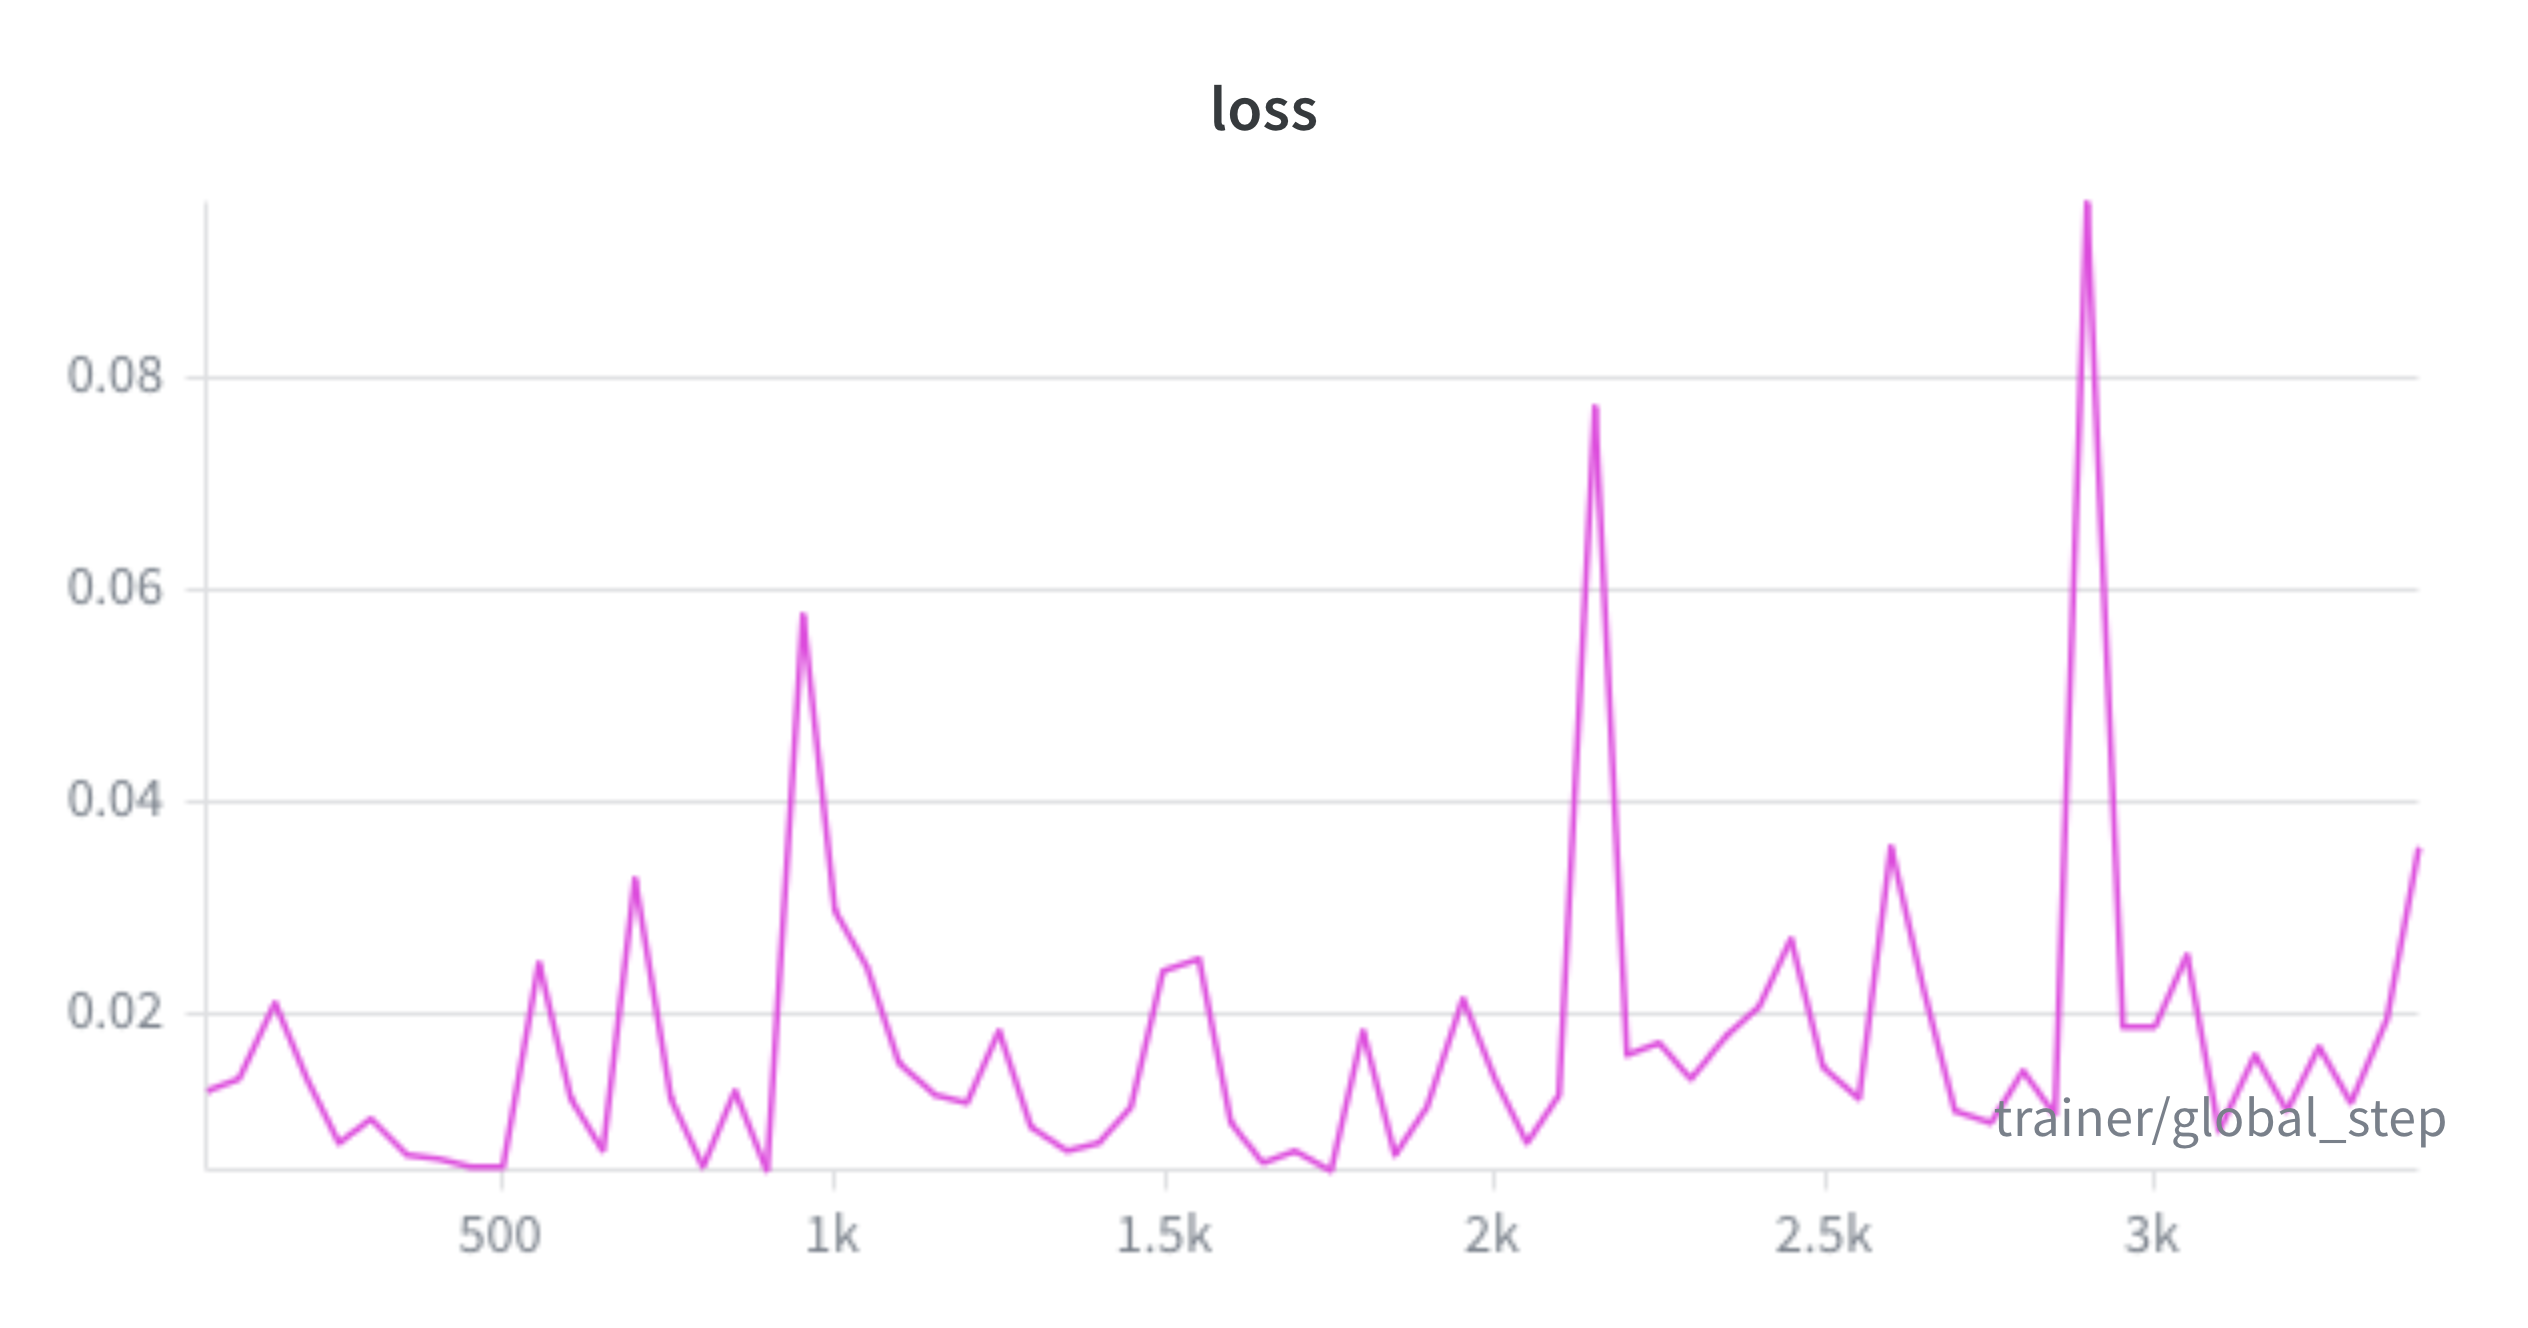
\includegraphics[width=5cm, height=4cm]{images/5-Experiments_and_results/Loss.png}
  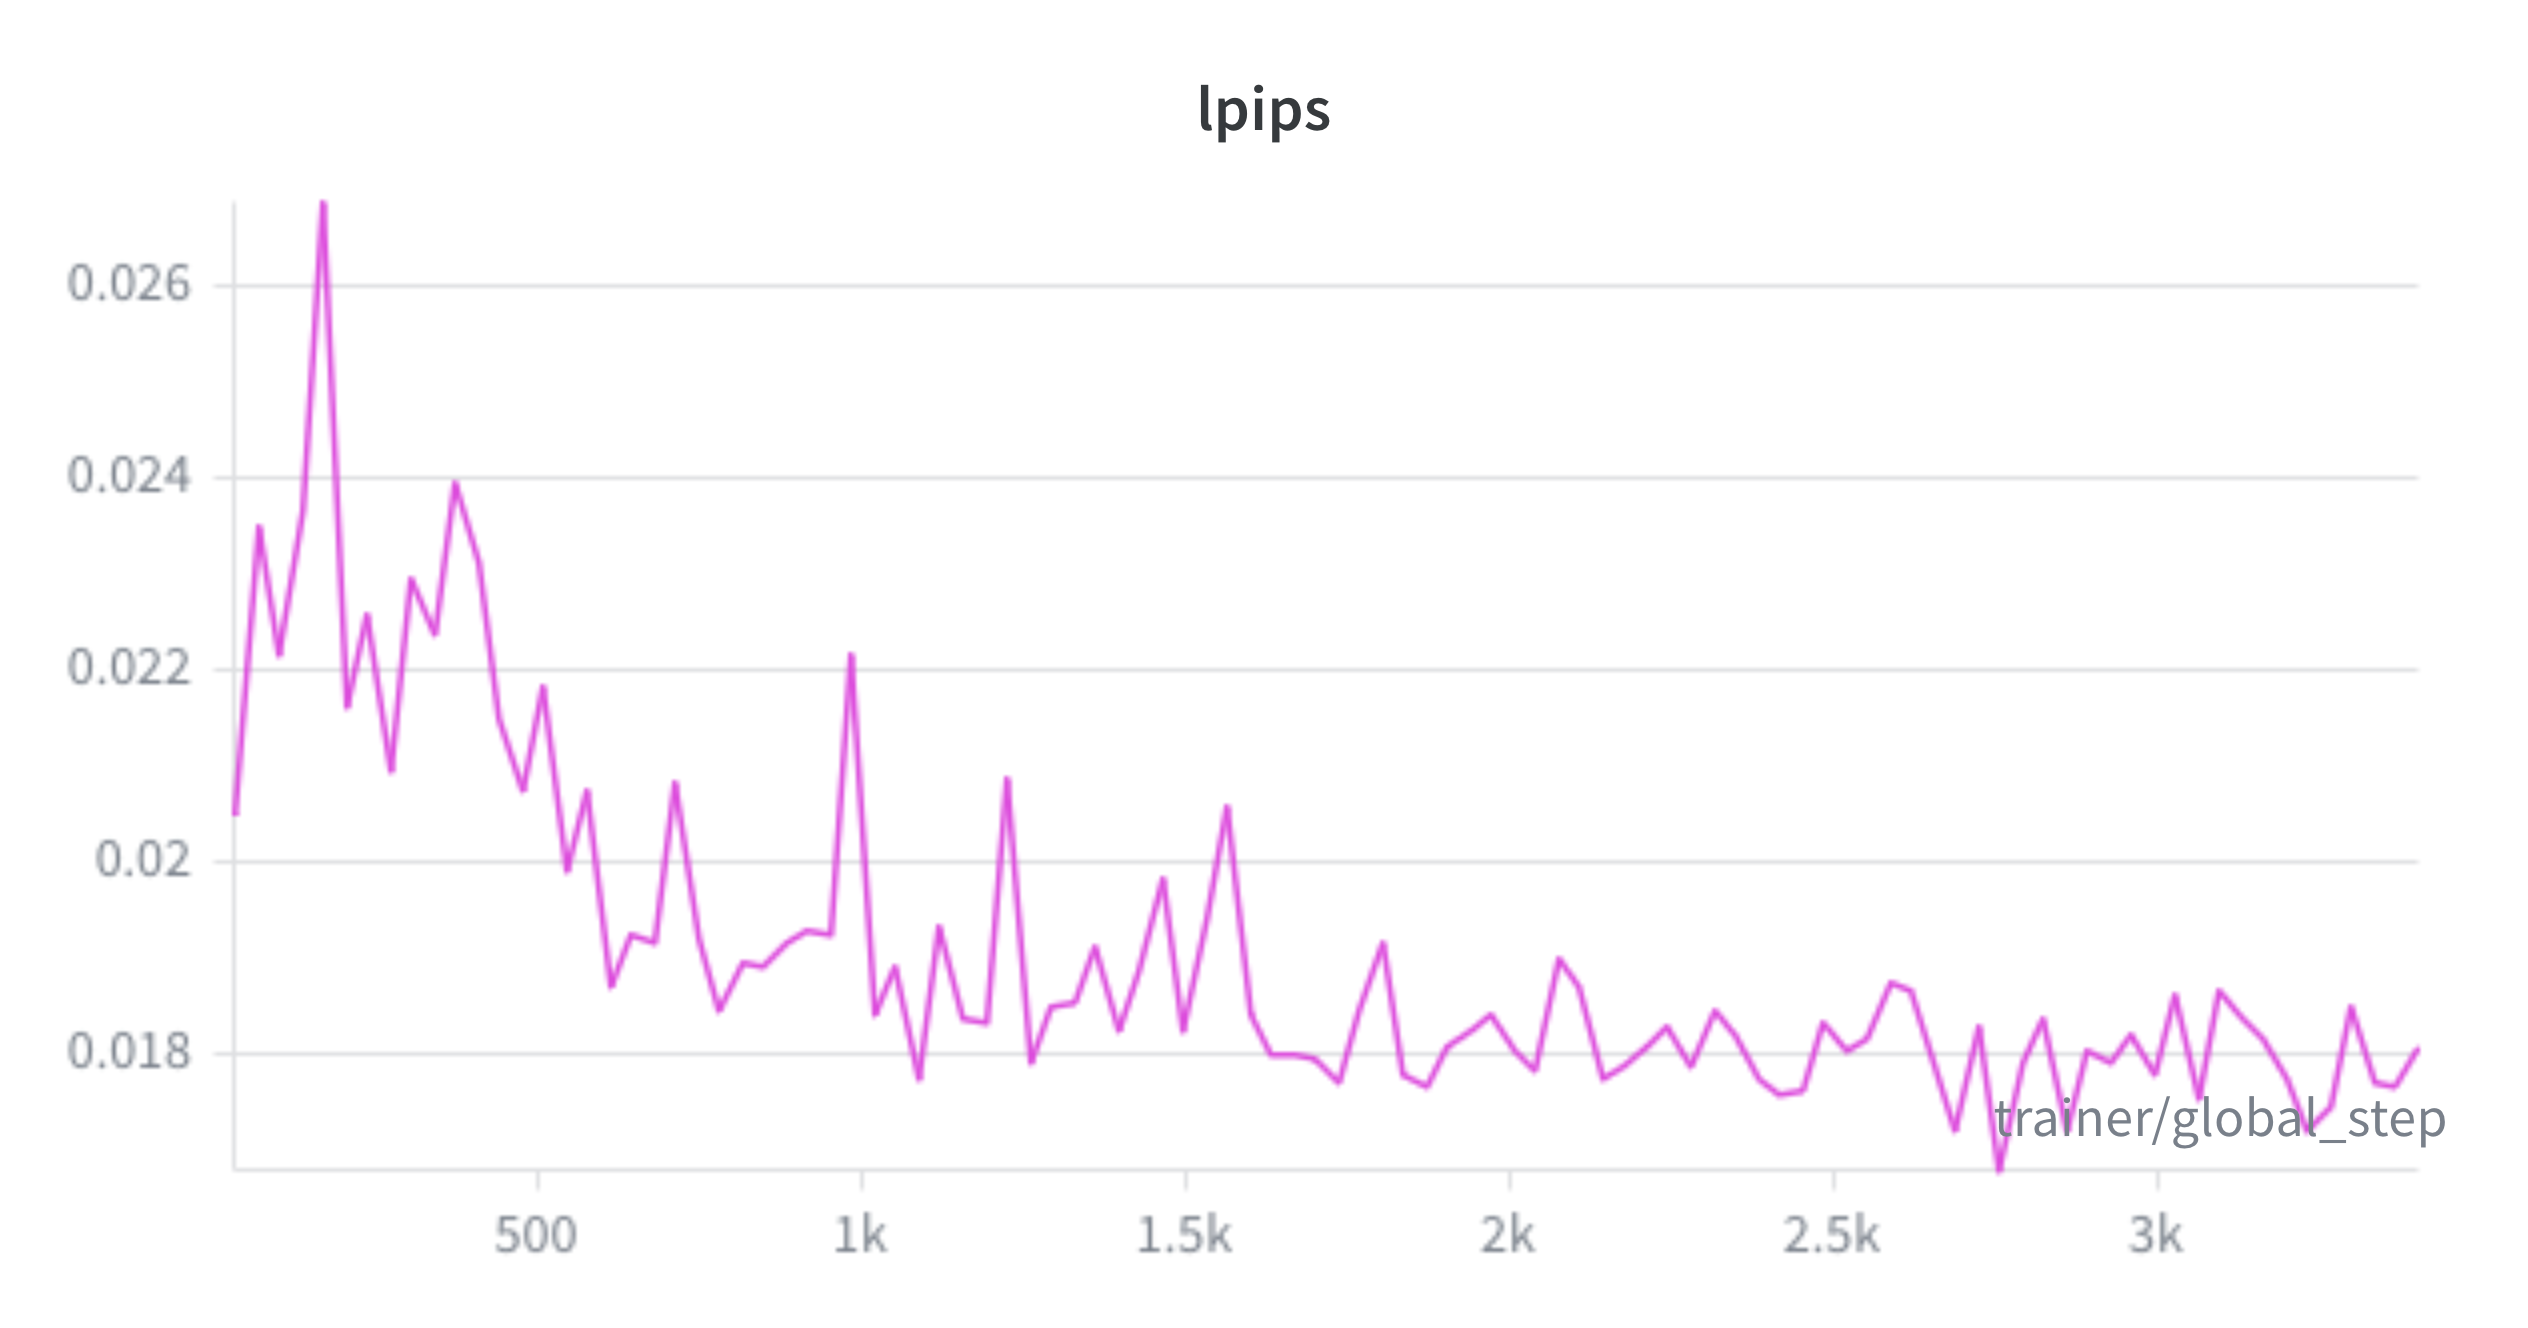
\includegraphics[width=5cm, height=4cm]{images/5-Experiments_and_results/LPIPS.png}
  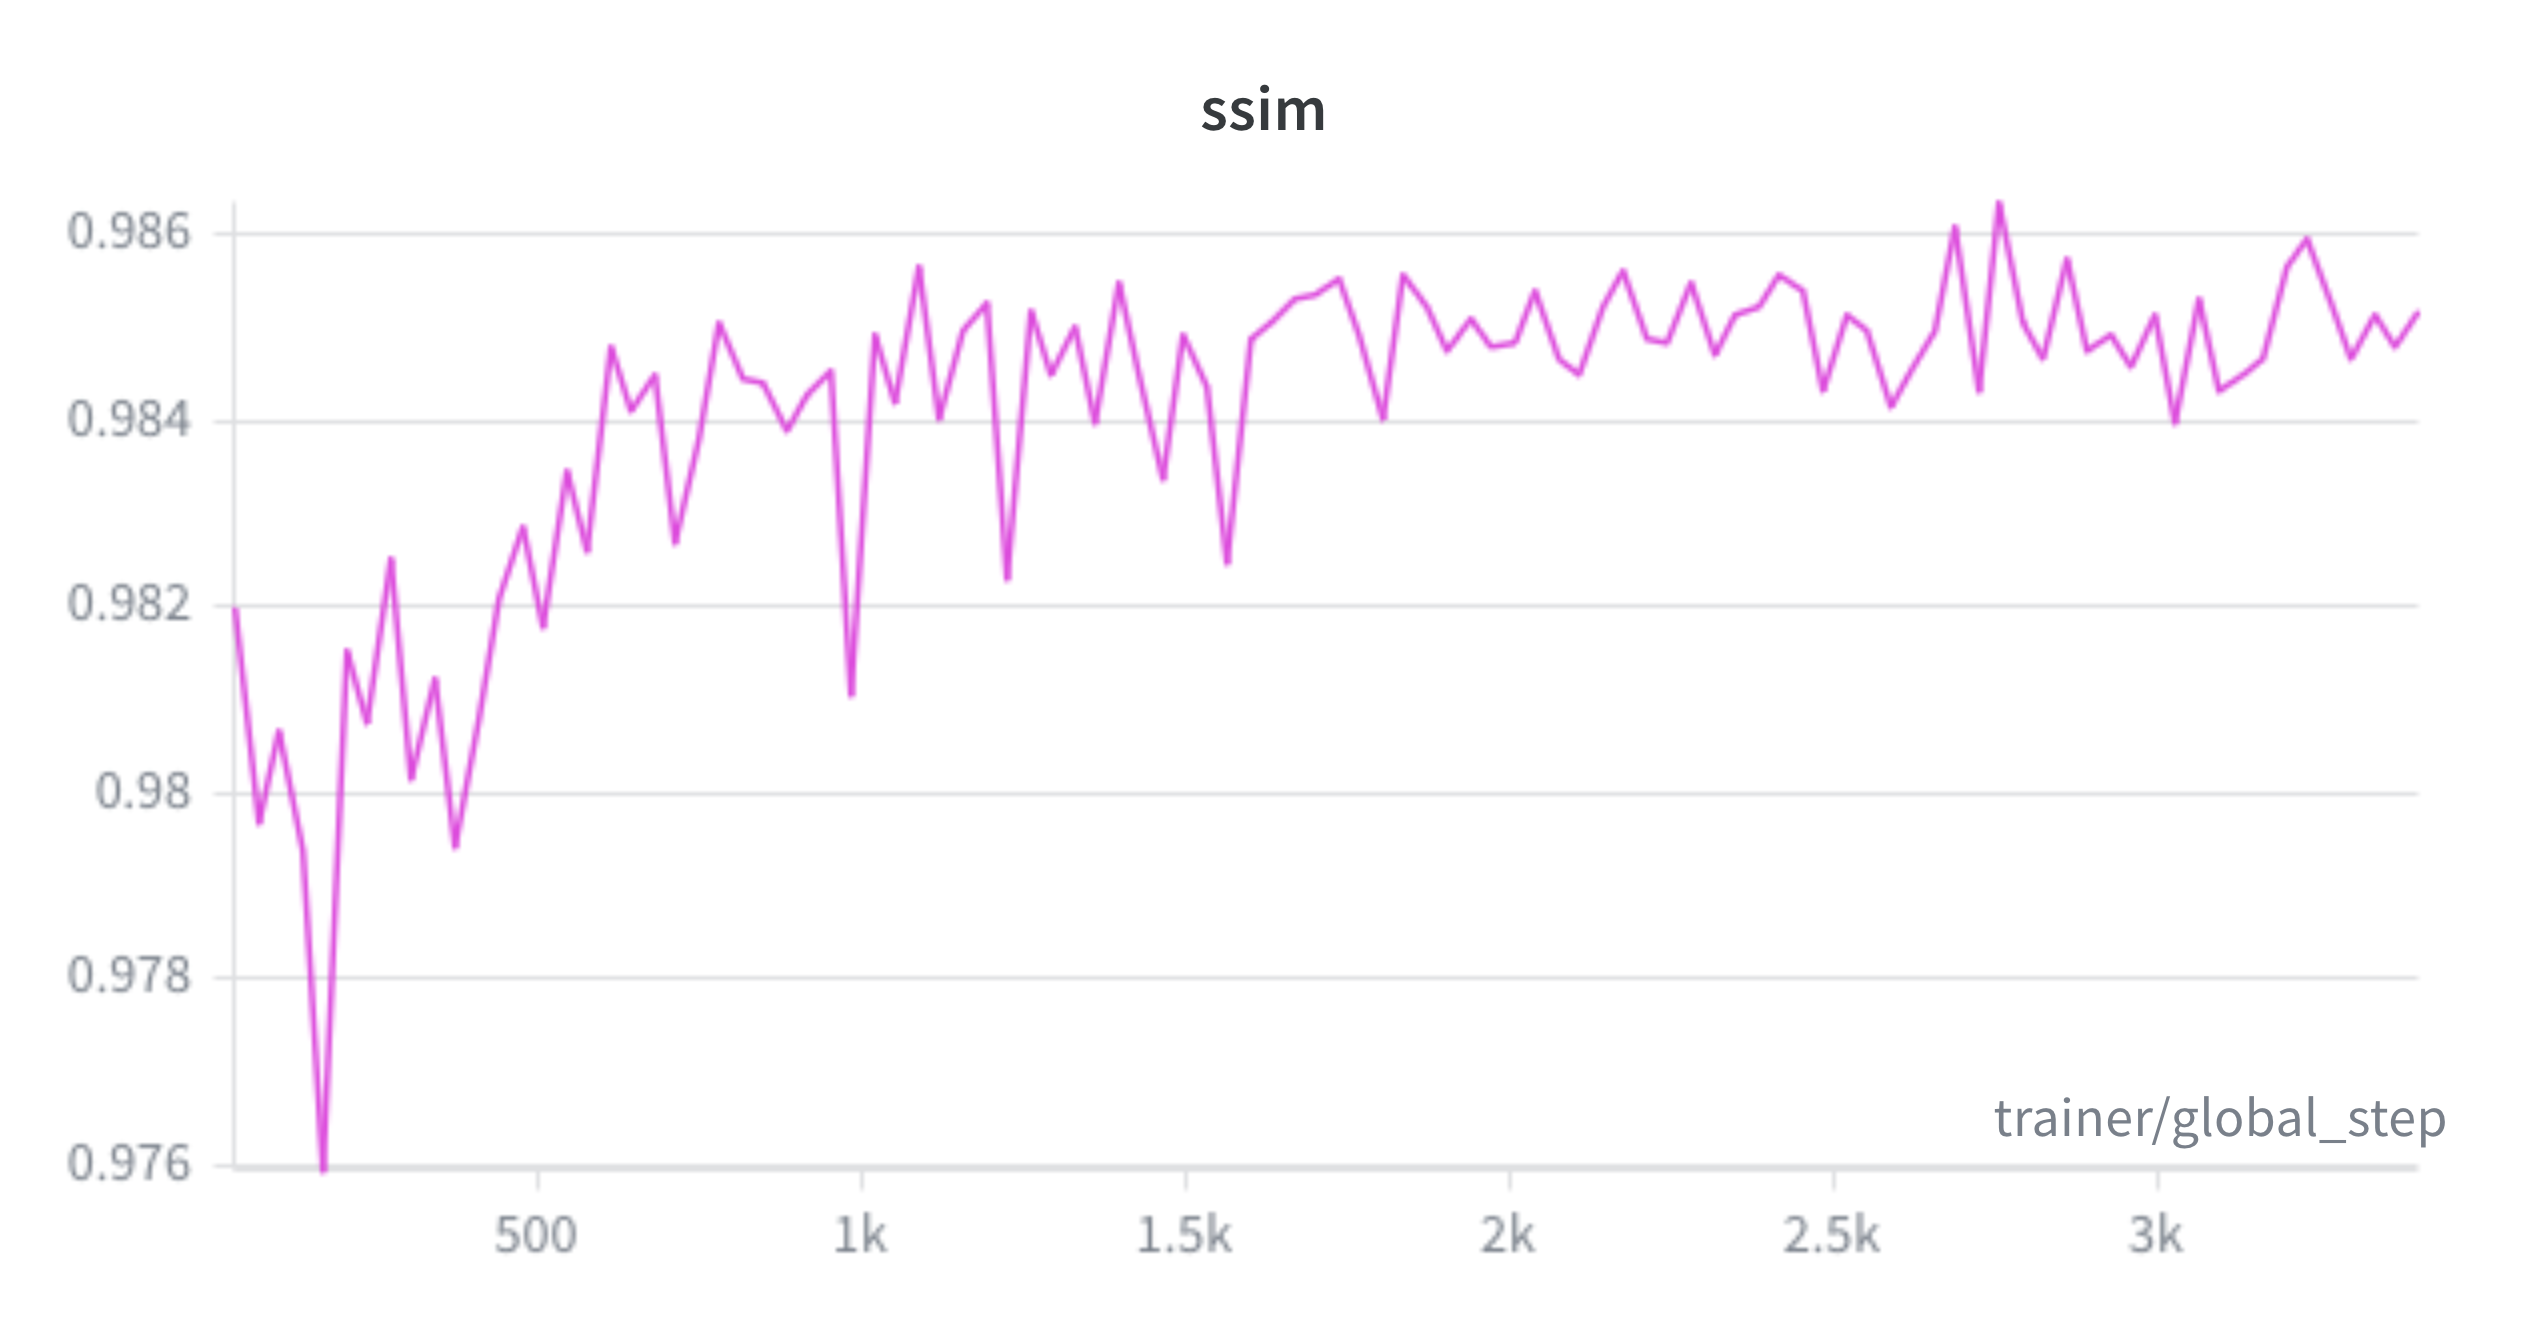
\includegraphics[width=5cm, height=4cm]{images/5-Experiments_and_results/SSIM.png}
  \caption{Courbe de la fonction de perte, de LPIPS et de SSIM de validation}
  \label{fig:courbe-loss-lpips-ssim}
\end{figure}


\section{Résultats par mouvement}

\subsection{Squat} \label{sec:resultats-squat}

Le squat constitue le mouvement le plus contraint visuellement, la barre chargée est portée sur le haut du dos, et les disques masquent en permanence une portion significative du torse, des épaules et parfois de la tête du sujet. Les montants du rack peuvent également apparaître en avant-plan dans la phase initiale du mouvement.

Le fine-tuning LoRA apporte une amélioration notable sur le squat (tableau~\ref{tab:resultats-squat}), avec une réduction de 24,5\,\% du LPIPS (0,0453 $\rightarrow$ 0,0342). Le gain en SSIM reste modéré (+0,43\,\%), ce qui est cohérent avec le comportement connu de cette métrique : le SSIM, fondé sur des statistiques locales de luminance et de contraste, est structurellement moins sensible aux différences de texture, de netteté des contours et de cohérence colorimétrique que LPIPS, dont les fonctionnalités profondes capturent davantage la plausibilité de la reconstruction.

\begin{table}[h]
  \centering
  \begin{tabular}{lccc}
    \hline
    \textbf{Modèle} & \textbf{SSIM} $\uparrow$ & \textbf{LPIPS} $\downarrow$ \\
    \hline
    TACO-baseline          & 0,977 & 0,0453 \\
    TACO-LoRA & \textbf{0,981} & \textbf{0,0342} \\
    \hline
  \end{tabular}
  \caption{Résultats quantitatifs sur la vidéo de \emph{squat}}
  \label{tab:resultats-squat}
\end{table}

\subsection{Développé couché} \label{sec:resultats-bench}

Le développé couché présente une géométrie d'occlusion particulière, la barre traverse horizontalement le champ de vision et masque le torse du sujet de façon quasi continue. La position allongée du sujet réduit également la surface visible exploitable comme indice de reconstruction.

Le développé couché présente l'amélioration la plus marquée de l'ensemble du jeu de données de test (tableau~\ref{tab:resultats-bench}), avec une réduction de 50,1\,\% du LPIPS (0,0792 $\rightarrow$ 0,0397) et un gain SSIM de 1,04\,\%. Ce résultat confirme l'hypothèse formulée au chapitre~\ref{ch_four} : l'occlusion quasi continue du torse constitue précisément le type de configuration pour lequel le fine-tuning spécialisé apporte le bénéfice le plus important. Le LPIPS baseline plus élevé (0,0792 contre 0,0453 au squat) reflète la difficulté intrinsèque de ce mouvement pour un modèle généraliste.

\begin{table}[h]
  \centering
  \begin{tabular}{lccc}
    \hline
    \textbf{Modèle} & \textbf{SSIM} $\uparrow$ & \textbf{LPIPS} $\downarrow$ \\
    \hline
    TACO-baseline          & 0,974 & 0,0792 \\
    TACO-LoRA & \textbf{0,984} & \textbf{0,0397} \\
    \hline
  \end{tabular}
  \caption{Résultats quantitatifs sur la vidéo de \emph{développé couché}}
  \label{tab:resultats-bench}
\end{table}

\subsection{Soulevé de terre} \label{sec:resultats-deadlift}

Le soulevé de terre offre une configuration intermédiaire, les disques sont visibles latéralement et masquent les jambes du sujet, mais le torse et la tête restent dégagés. La trajectoire verticale de la barre et la durée relativement courte des phases concentriques limitent la durée des occlusions.

Le soulevé de terre constitue le cas le moins favorable au fine-tuning (tableau~\ref{tab:resultats-deadlift}) : le LPIPS reste quasi identique entre le modèle baseline (0,0487) et le modèle fine-tuné (0,0489), soit une différence de 0,0002. Le gain SSIM est également très faible (+0,22\,\%). Ce résultat est cohérent avec les occlusions de ce mouvement : les disques masquent principalement les membres inférieurs latéralement, laissant le torse et la tête dégagés, ce qui limite l'apport du fine-tuning spécialisé.

\begin{table}[h]
  \centering
  \begin{tabular}{lccc}
    \hline
    \textbf{Modèle} & \textbf{SSIM} $\uparrow$ & \textbf{LPIPS} $\downarrow$ \\
    \hline
    TACO-baseline          & 0,959 & \textbf{0,0487} \\
    TACO-LoRA & \textbf{0,961} & 0,0489 \\
    \hline
  \end{tabular}
  \caption{Résultats quantitatifs sur la vidéo du \emph{soulevé de terre}}
  \label{tab:resultats-deadlift}
\end{table}

\section{Comparaison avant / après fine-tuning}

\subsection{Synthèse quantitative globale}

Le tableau~\ref{tab:resultats-globaux} agrège les résultats des trois mouvements et présente la performance moyenne sur l'ensemble du jeu de données de test.

\begin{table}[h]
  \centering
  \begin{tabular}{lccc}
    \hline
    \textbf{Modèle} & \textbf{SSIM} $\uparrow$ & \textbf{LPIPS} $\downarrow$ \\
    \hline
    TACO-baseline          & 0,970 & 0,0577 \\
    TACO-LoRA & 0,975 & 0,0375 \\
    \hline
    \textbf{Gain absolu}   & +0,005 & $-$0,020 \\
    \textbf{Gain relatif}  & +0,52\,\% & $-$35,0\,\% \\
    \hline
  \end{tabular}
  \caption{Résultats globaux sur l'ensemble du jeu de données de test (3 clips)}
  \label{tab:resultats-globaux}
\end{table}

Sur l'ensemble du jeu de données de test (1\,199 trames issues de 3 vidéos couvrant les trois mouvements de référence), le fine-tuning LoRA améliore le LPIPS de 35,0\,\% en moyenne. Le gain en SSIM est plus modeste (+0,52\,\%), ce qui est attendu, LPIPS est davantage aligné avec la perception humaine de la qualité de reconstruction que le SSIM, qui opère sur des statistiques locales de luminance et de contraste.

\subsection{Significativité statistique}

Pour vérifier que les écarts observés entre le modèle baseline et le modèle fine-tuné ne sont pas attribuables au hasard, un test de Wilcoxon apparié~\cite{Wilcoxon-1945} est conduit trame par trame sur les 1\,199 trames du jeux de données de test. Les valeurs $p$ obtenues sont les suivantes :

\begin{itemize}
  \item SSIM  : $p = 1{,}45 \times 10^{-96}$
  \item LPIPS : $p = 3{,}28 \times 10^{-5}$
\end{itemize}

Les deux tests rejettent l'hypothèse nulle avec $\alpha = 0{,}05$. Ces résultats doivent néanmoins être interprétés avec précaution : les 1\,199 trames provenant de seulement 3 vidéos d'un unique sujet, les observations ne sont pas strictement indépendantes (corrélation temporelle intra-vidéo), ce qui tend à gonfler artificiellement la significativité statistique. Ces résultats sont donc indicatifs plutôt que conclusifs, et devront être confirmés sur un jeu de données de test plus large et plus diversifié.

\subsection{Analyse qualitative comparative}

Les figures~\ref{fig:qual-squat}, \ref{fig:qual-bench} et \ref{fig:qual-deadlift} présentent, pour chacun des trois mouvements, une trame représentative sous quatre conditions : référence non-occluse (A), entrée occluse (B), reconstruction TACO-baseline (C), reconstruction TACO-LoRA (D).

Au squat (figure~\ref{fig:qual-squat}), l'occlusion porte principalement sur l'épaule droite et la partie supérieure du torse, masquées par le disque. TACO-baseline produit une reconstruction de l'épaule et du torse floue avec une colorimétrie dégradée du \textit{singlet}. TACO-LoRA restitue une silhouette plus nette et une continuité du tissu cohérente avec les trames adjacentes.

\begin{figure}[htp]
  \centering
  
\includegraphics[width=3cm, height=5cm]{images/5-Experiments_and_results/Squat.png}
  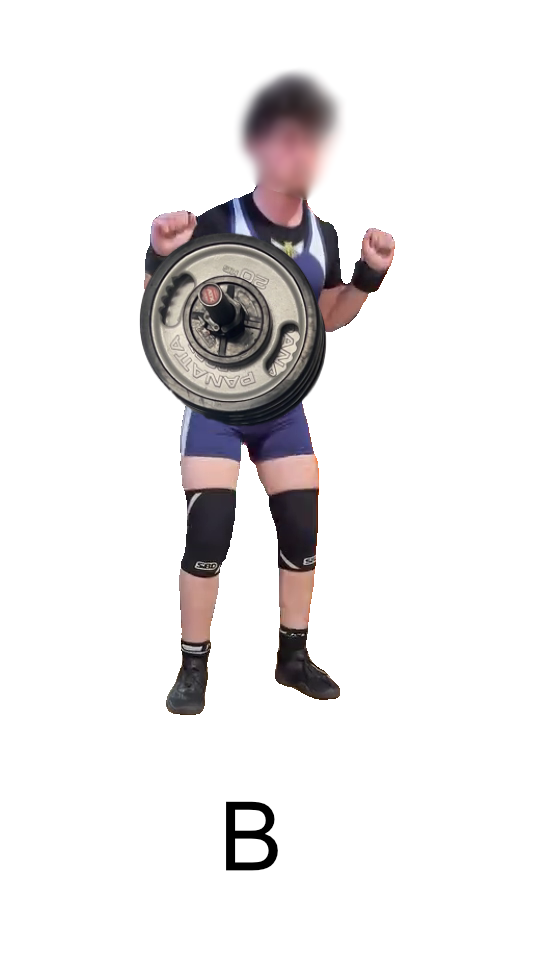
\includegraphics[width=3cm, height=5cm]{images/5-Experiments_and_results/Squat-occlusion.png}
  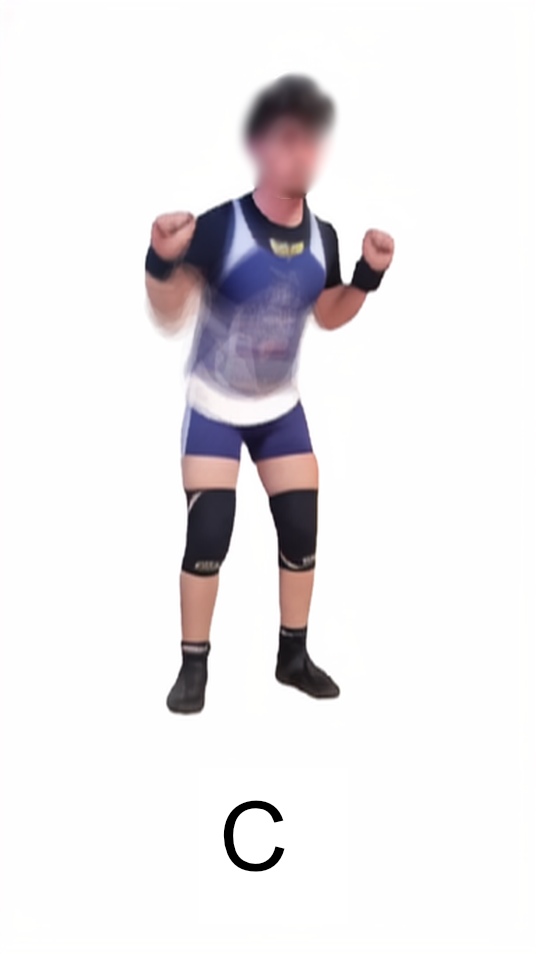
\includegraphics[width=3cm, height=5cm]{images/5-Experiments_and_results/Squat-baseline.png}
  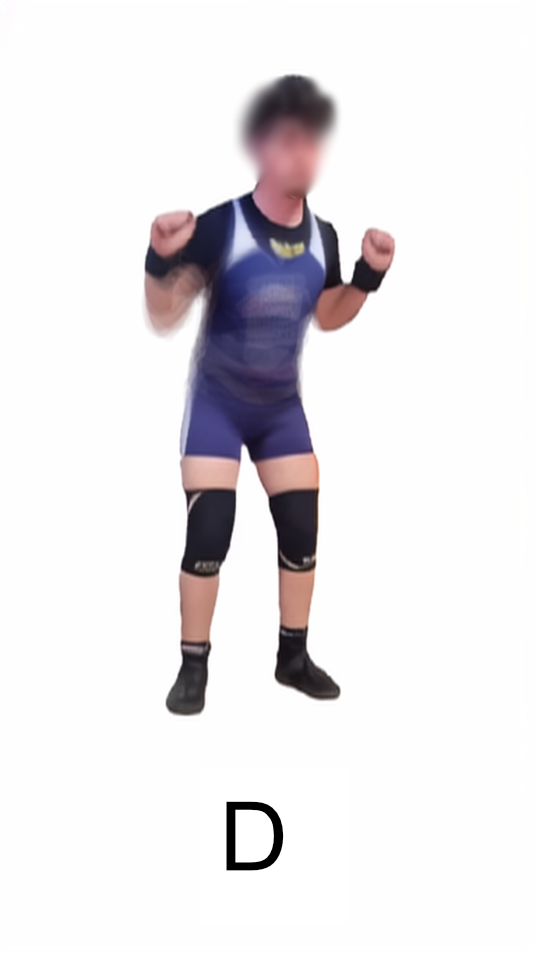
\includegraphics[width=3cm, height=5cm]{images/5-Experiments_and_results/Squat-lora.png}
  \caption{Comparaisons visuelles au squat}
  \label{fig:qual-squat}
\end{figure}

Au développé couché (figure~\ref{fig:qual-bench}), la sécurité masque quasi intégralement le torse sur toute la durée du mouvement. TACO-baseline laisse subsister une zone grisée incohérente au centre de la reconstruction, révélant une incertitude élevée du modèle généraliste face à cette situation. TACO-LoRA produit un torse reconstruit plus plausible, avec une continuité de l'habillement préservée entre les trames consécutives. Ce contraste est cohérent avec la réduction de 50,1\,\% du LPIPS observée sur ce mouvement.

\begin{figure}[htp]
  \centering
  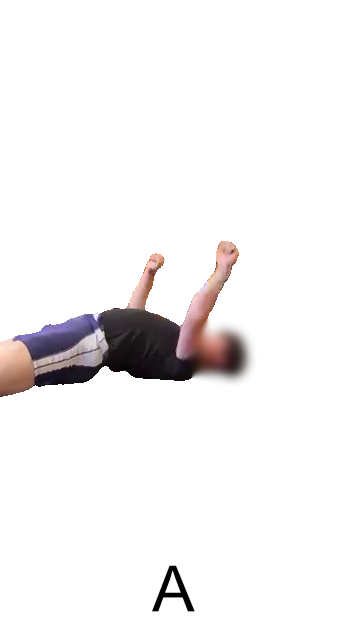
\includegraphics[width=3cm, height=5cm]{images/5-Experiments_and_results/Bench.png}
  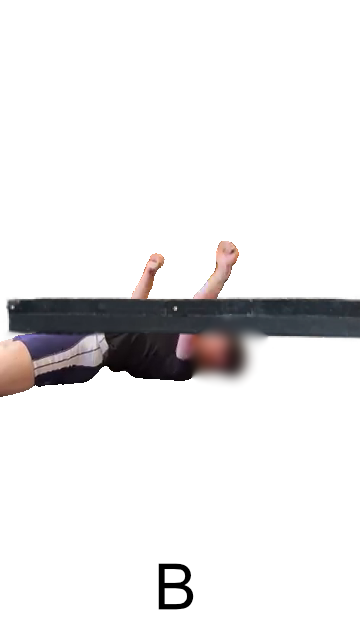
\includegraphics[width=3cm, height=5cm]{images/5-Experiments_and_results/Bench-occlusion.png}
  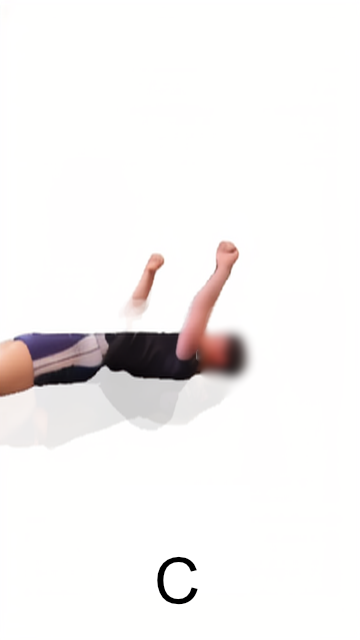
\includegraphics[width=3cm, height=5cm]{images/5-Experiments_and_results/Bench-baseline.png}
  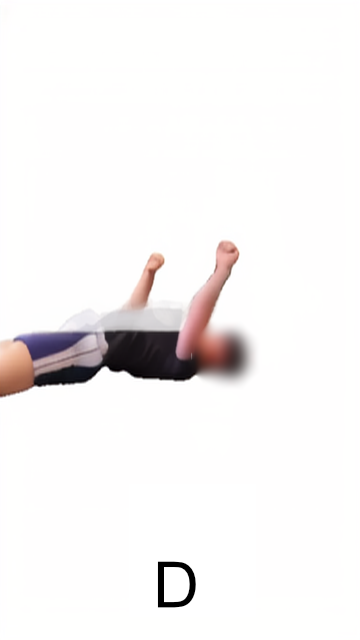
\includegraphics[width=3cm, height=5cm]{images/5-Experiments_and_results/Bench-lora.png}
  \caption{Comparaisons visuelles au développé couché}
  \label{fig:qual-bench}
\end{figure}

Au soulevé de terre (figure~\ref{fig:qual-deadlift}), le disque masque la région pelvienne et le haut des cuisses. Les reconstructions TACO-baseline et TACO-LoRA sont visuellement proches, ce qui est cohérent avec l'absence d'amélioration métrique significative sur ce mouvement ($\Delta$LPIPS = +0,0002).

\begin{figure}[htp]
  \centering
  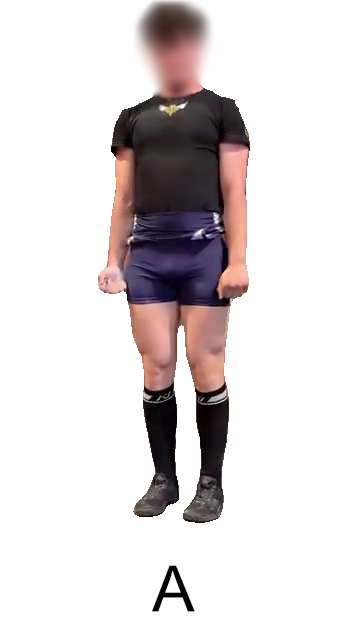
\includegraphics[width=3cm, height=5cm]{images/5-Experiments_and_results/Deadlift.png}
  
\includegraphics[width=3cm, height=5cm]{images/5-Experiments_and_results/Deadlift-occlusion.png}
  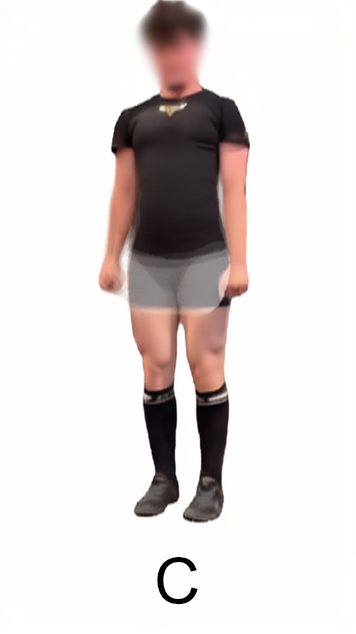
\includegraphics[width=3cm, height=5cm]{images/5-Experiments_and_results/Deadlift-baseline.png}
  
\includegraphics[width=3cm, height=5cm]{images/5-Experiments_and_results/Deadlift-lora.png}
  \caption{Comparaisons visuelles au soulevé de terre}
  \label{fig:qual-deadlift}
\end{figure}

\section{Analyse du cas limite}

\subsection{Occlusions massives et prolongées}

Lorsque la part occluse dépasse approximativement 60\,\% du sujet (figure~\ref{fig:big-occlusion-limitation}) sur une fenêtre temporelle longue (au-delà de la fenêtre d'inférence native de 14 trames de TACO, le modèle perd les indices visuels nécessaires à une reconstruction fidèle et tend à produire des solutions "hallucinées" plausibles mais infidèles~\cite{TACO-2025}). Le cas typique est celui d'un développé couché vu de côté où les disques cachent intégralement les bras du sujet sur l'ensemble du mouvement concentrique. Une stratégie d'atténuation envisagée est la propagation explicite d'informations depuis les trames pré- et post-occlusion via un mécanisme d'attention étendue, à l'image de l'approche proposée par ProPainter~\cite{ProPainter-2023}.

\begin{figure}[htp]
  \centering
  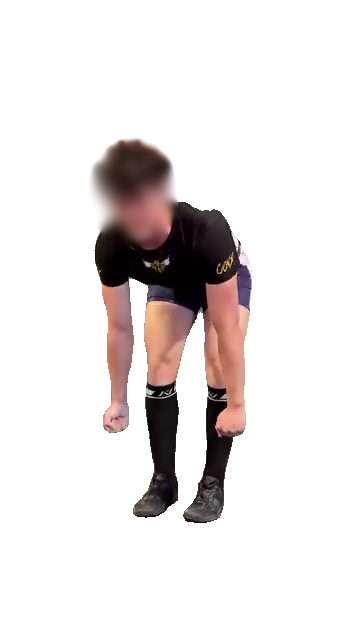
\includegraphics[width=3cm, height=5cm]{images/5-Experiments_and_results/Big-occlusion-frame.png}
  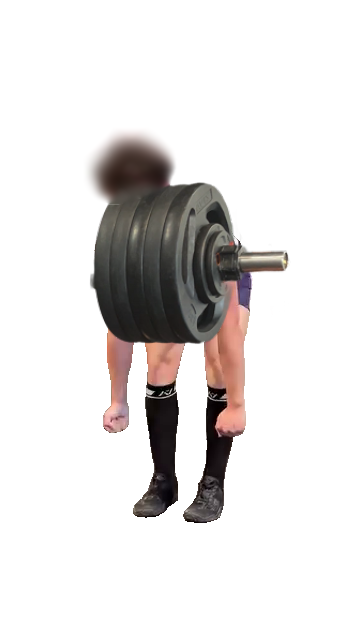
\includegraphics[width=3cm, height=5cm]{images/5-Experiments_and_results/Big-occlusion-frame-occluded.png}
  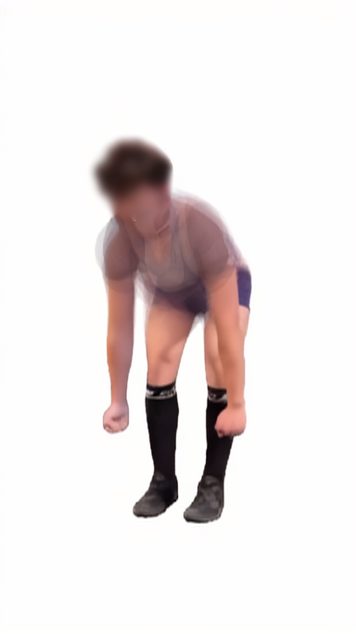
\includegraphics[width=3cm, height=5cm]{images/5-Experiments_and_results/Big-occlusion-frame-lora.png}
  \caption{Hallucination avec une occlusion massive et prolongée}
  \label{fig:big-occlusion-limitation}
\end{figure}

\section{Discussion et comparaison à l'état de l'art}

\subsection{Positionnement par rapport à TACO original}

Les auteurs de TACO rapportent, sur leur benchmark OvO-Hard, un LPIPS moyen de 0,142~\cite{TACO-2025} sur des séquences d'objets génériques. Sur le benchmark powerlifting, le modèle baseline atteint 0,058 en LPIPS moyen, une valeur nettement inférieure qui s'explique par la nature du domaine : les séquences de force athlétique du dataset présentent un sujet isolé sur fond blanc, une géométrie d'occlusion répétitive et des textures vestimentaires relativement homogènes, ces conditions sont plus favorables que les objets génériques du dataset OvO.

Après fine-tuning LoRA, notre modèle atteint 0,038 en LPIPS, soit une amélioration de 35,0\,\% sur le domaine ciblé. C'est cohérent avec ce que la littérature rapporte pour des fine-tunings LoRA spécialisés sur des modèles de diffusion vidéo~\cite{LoRA-2021} : on rapporte des gains de l'ordre de 20 à 40\,\% sur des tâches de génération spécialisées avec des rangs comparables ($r = 16$), et des travaux appliquant LoRA à Stable Diffusion pour des domaines visuels restreints confirment qu'un dataset de quelques dizaines de séquences suffit à produire une adaptation significative lorsque le modèle de base est déjà bien initialisé~\cite{DreamBooth-2023}.

\subsection{Comparaison avec les alternatives discutées}

Une comparaison formelle avec pix2gestalt et ProPainter n'a pas été conduite dans ce travail. Les arguments avancés au chapitre~\ref{ch_three} restent donc indicatifs plutôt que quantitativement validés. Néanmoins, les résultats obtenus sur TACO permettent de formuler deux observations.

D'une part, la cohérence temporelle native de TACO constitue un avantage structurel difficile à quantifier sur une métrique trame-à-trame comme LPIPS, mais visible qualitativement dans la stabilité des reconstructions entre trames consécutives. D'autre part, ProPainter~\cite{ProPainter-2023} requiert les masques d'occlusion en entrée, ce qui suppose de savoir a priori quelles régions du sujet sont masquées, un problème que TACO résout précisément via la complétion amodale. Une comparaison directe entre les deux méthodes constitue une perspective pour les travaux futurs.

\section{Résultats et Discussion} \label{sec:implications-pipeline}

Le tableau~\ref{tab:mpjpe} présente le MPJPE (\textit{Mean Per-Joint Position Error}) calculé entre la reconstruction 3D produite par SAM 3D Body sur les images de référence avant l'occlusion (\textit{ground truth}), les images occluses brutes, les sorties TACO-baseline, et les sorties TACO-LoRA.

\begin{table}[h]
  \centering
  \begin{tabular}{lccc}
    \hline
    \textbf{Mouvement} & \textbf{Occlus} & \textbf{TACO-baseline} & \textbf{TACO-LoRA} \\
                       & MPJPE (mm)      & MPJPE (mm)             & MPJPE (mm) \\
    \hline
    Squat              & $\mathbf{43{,}7 \pm 26{,}5}$ & $48{,}0 \pm 21{,}1$ & $47{,}3 \pm 21{,}5$ \\
    Développé couché   & $38{,}0 \pm 24{,}1$ & $43{,}4 \pm 21{,}1$ & $\mathbf{37{,}2 \pm 17{,}6}$ \\
    Soulevé de terre   & $\mathbf{94{,}3 \pm 40{,}1}$ & $181{,}8 \pm 143{,}1$ & $108{,}0 \pm 54{,}2$ \\
    \hline
  \end{tabular}
  \caption{MPJPE (mm) entre la reconstruction 3D et le ground truth, pour les trois conditions d'entrée de SAM 3D Body. Les valeurs indiquent la moyenne ainsi que l'écart-type ($\pm$) sur l'ensemble des trames de chaque mouvement.}
  \label{tab:mpjpe}
\end{table}

La figure~\ref{fig:mpjpe-boxplot} présente la distribution du MPJPE sous forme de boîtes à moustaches, révélant non seulement les tendances centrales mais également la dispersion et la présence de valeurs extrèmes pour chaque condition.

\begin{figure}[htp]
  \centering
  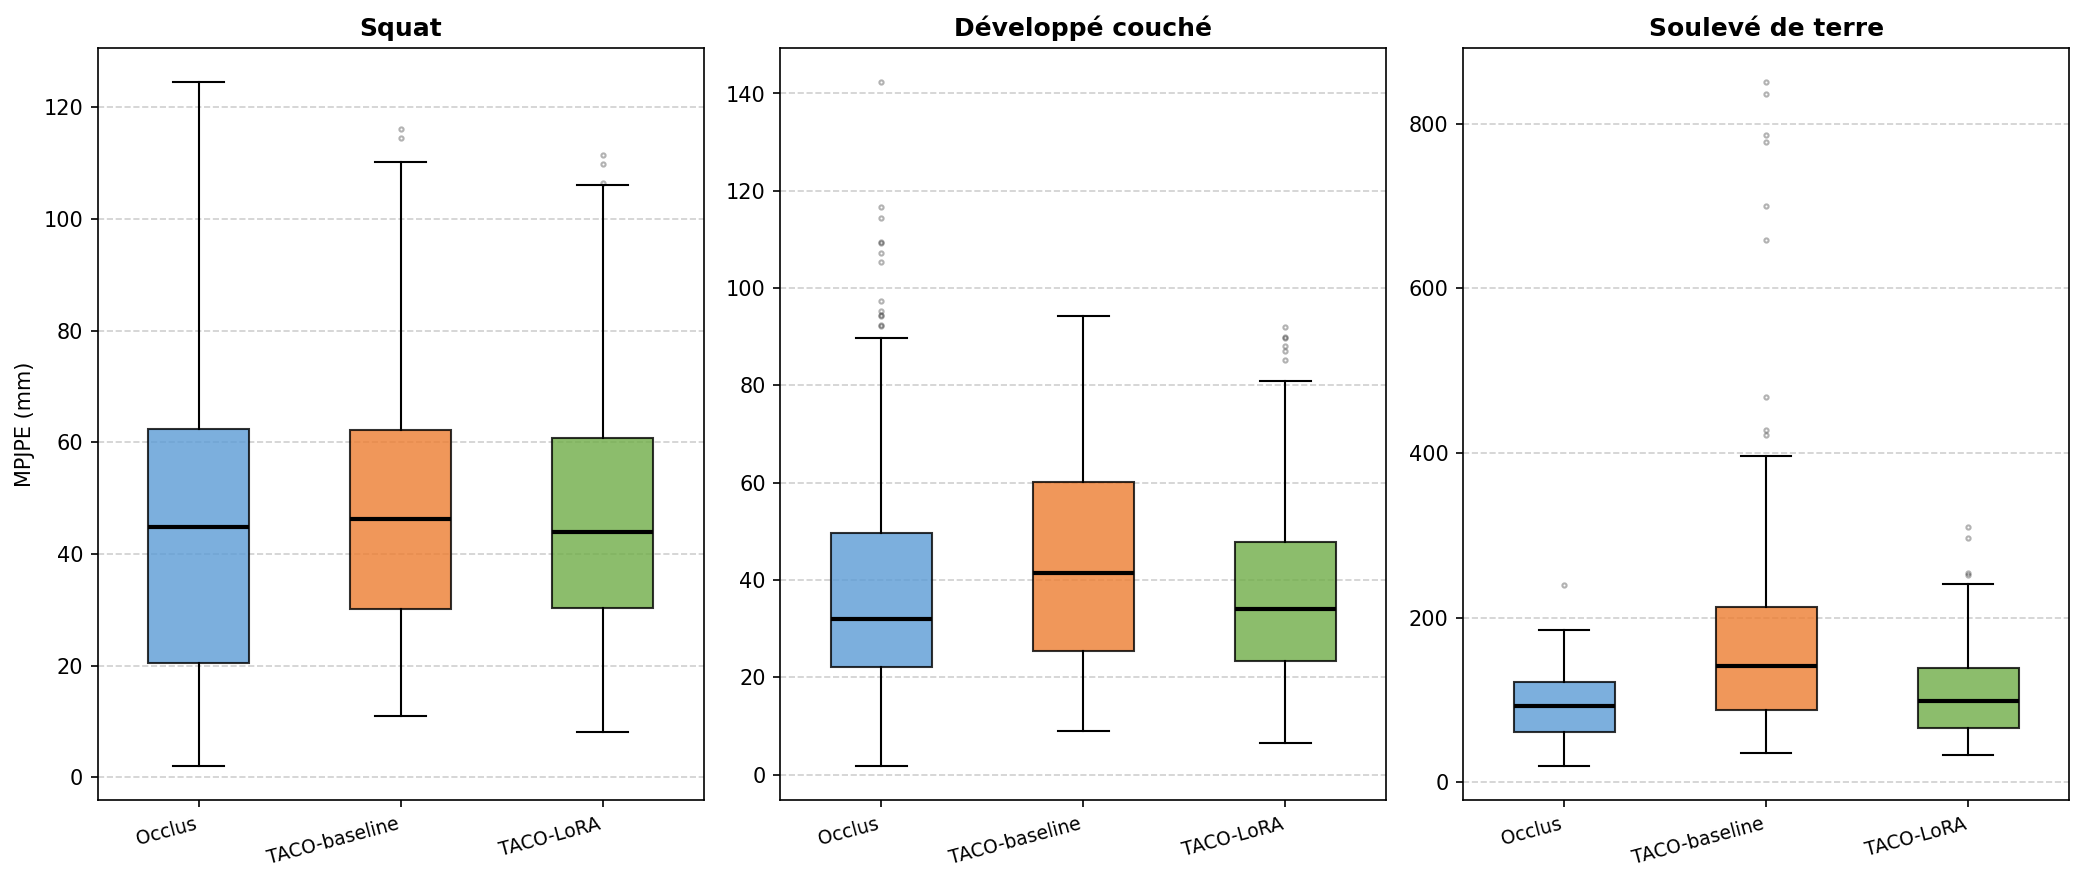
\includegraphics[width=14cm, height=6.5cm]{images/5-Experiments_and_results/mpjpe-boxplot.png}
  \caption{Distribution du MPJPE pour les trois conditions d'entrée de SAM 3D Body}
  \label{fig:mpjpe-boxplot}
\end{figure}

Trois observations se dégagent. Premièrement, au développé couché, TACO-LoRA atteint un MPJPE de 37,2~mm, légèrement inférieur à celui obtenu sur l'image occluse brute (38,0~mm), confirmant que la complétion amodale améliore effectivement la reconstruction 3D sur ce mouvement. Deuxièmement, au soulevé de terre, TACO-baseline produit une erreur particulièrement élevée (181,8~mm, avec un écart-type de 143~mm révélateur d'une forte instabilité), tandis que TACO-LoRA ramène cette erreur à 108,0~mm, soit une réduction de 40,6\,\% par rapport au baseline. Ce résultat suggère que le fine-tuning spécialisé stabilise les reconstructions dans les configurations d'occlusion les plus difficiles pour le modèle généraliste. Troisièmement, au squat, l'amélioration apportée par TACO-LoRA reste marginale ($-$0,7~mm par rapport au baseline), cohérente avec les résultats 2D de la section~\ref{sec:resultats-squat}.

Il convient de noter que, pour les trois mouvements, TACO-LoRA n'améliore pas systématiquement le MPJPE par rapport à l'image occluse brute (+3,6~mm au squat, +13,7~mm au soulevé de terre). Ce résultat indique que la complétion amodale, même améliorée par le fine-tuning, peut introduire des artefacts visuels suffisamment importants pour perturber SAM 3D Body davantage que l'occlusion originale. Cette limite est discutée dans la section~\ref{sec:limites}.

\medskip
Le chapitre suivant tire les conclusions générales de ce travail et identifie les pistes d'amélioration et d'extension les plus prometteuses pour la suite du développement de ce pipeline.
% ===============================================
% CONCLUSION ET PERSPECTIVES
% ===============================================

\chapter{Conclusion et perspectives} \label{ch_six}

\section{Bilan}

Ce mémoire a présenté la conception, l'implémentation et l'évaluation d'un pipeline modulaire de reconstruction 3D des mouvements de force athlétique à partir de vidéos monoculaires non calibrées. L'objectif central était de proposer une méthode accessible, sans marqueurs physiques ni d'infrastructure multicaméras, capable de gérer explicitement les occlusions générées par l'équipement de force athlétique.

Quatre contributions principales ont été développées au cours de ce travail.

Premièrement, un pipeline séquentiel opérationnel intégrant quatre modèles de l'état de l'art (SAM3, MoGe-2, TACO, SAM 3D Body) a été conçu. Cette architecture permet de passer d'une vidéo brute filmée en salle de musculation à un maillage 3D complet du corps de l'athlète, incluant le corps, les mains et les pieds, sans marqueurs physiques ni calibration préalable de la caméra. Le découpage modulaire facilite le remplacement de chaque composant au fil des avancées de l'état de l'art.

Deuxièmement, un dataset spécialisé pour la force athlétique a été constitué, regroupant des séquences comprenant les trois mouvements de référence (squat, développé couché, soulevé de terre) issues de six sujets distincts. Les occlusions synthétiques ont été générées via une banque d'occlusions spécialisée (disques IPF, disques de salle commerciale, racks à squat), et huit augmentations visuelles ont été appliquées sur les vidéos sources pour pallier la taille restreinte du corpus. La méthodologie de construction, entièrement automatisée et réutilisant les premiers modules du pipeline d'inférence, garantit la cohérence entre les distributions d'entraînement et d'inférence.

Troisièmement, un fine-tuning LoRA de TACO sur ce dataset a été conduit et évalué quantitativement. Sur un jeu de données de test composé de trois séquences d'un sujet absent du dataset d'entraînement, le modèle fine-tuné améliore le LPIPS de 35,0\,\% en moyenne par rapport au modèle baseline ($0{,}0577 \rightarrow 0{,}0375$), avec une significativité statistique confirmée par un test de Wilcoxon ($p = 3{,}28 \times 10^{-5}$). L'amélioration est particulièrement marquée au développé couché ($-50{,}1\,\%$ de LPIPS), mouvement pour lequel l'occlusion quasi continue du torse constitue précisément le cas d'usage ciblé par le fine-tuning. L'évaluation via le MPJPE confirme que cette amélioration a un impact en aval sur la reconstruction 3D : au développé couché, TACO-LoRA atteint un MPJPE de 37,2~mm, légèrement inférieur à celui obtenu sur l'image occluse brute (38,0~mm), et au soulevé de terre, le fine-tuning réduit l'erreur de 40,6\,\% par rapport au baseline (108,0~mm contre 181,8~mm).

Quatrièmement, une interface web de visualisation a été développée, permettant d'explorer les maillages 3D produits par SAM 3D Body et de calculer automatiquement les indicateurs biomécaniques pertinents pour chaque mouvement : profondeur du squat, verrouillage des coudes et des genoux, inclinaison du buste, et asymétrie des hanches. Cette interface constitue le premier maillon applicatif concret du pipeline.

\section{Limites} \label{sec:limites}

Plusieurs limites du pipeline développé doivent être reconnues.

\textbf{Taille modeste du jeu de données de test.} L'évaluation quantitative repose sur trois séquences issues d'un unique sujet, couvrant une diversité restreinte de morphologies, d'éclairages et de configurations de salle. Les résultats doivent donc être considérés comme indicatifs plutôt que définitifs, et leur généralisation à d'autres sujets et conditions de capture reste à valider sur un corpus plus large.

\textbf{Distribution d'occlusions identique entre entraînement et test.} Les séquences du jeu de données de test ont été occluses en utilisant la même banque d'occlusions synthétiques (disques IPF, racks) et le même pipeline de génération que les séquences d'entraînement. Cette homogénéité dans la distribution des occlusions favorise mécaniquement le modèle fine-tuné, qui a été spécifiquement entraîné sur ce type d'artefact. La performance sur des occlusions réelles de compétition, dont l'apparence (perspective, ombres portées, reflets) diffère nécessairement des occlusions synthétiques, reste donc à valider.

\textbf{Évaluation perceptive humaine absente.} Aucune étude utilisateur n'a été menée auprès d'un panel d'entraîneurs ou d'arbitres afin d'évaluer la qualité perçue des reconstructions. La validation repose exclusivement sur des métriques automatiques (LPIPS, SSIM, MPJPE). LPIPS corrèle mieux que SSIM avec le jugement humain mais ne le remplace pas, des reconstructions anatomiquement plausibles peuvent obtenir un bon LPIPS tout en présentant des artefacts subtils détectables à l'œil.

\textbf{Absence de comparaison avec un fine-tuning complet.} Le coût computationnel d'un fine-tuning complet de TACO étant prohibitif sur le matériel disponible ($2 \times$ RTX A5000 contre $8 \times$ H100 requis), l'écart de performance entre l'adaptation LoRA et un fine-tuning complet ne peut être quantifié dans ce travail. Il est raisonnable de supposer qu'un fine-tuning complet apporterait un gain supplémentaire, au prix d'un risque accru de catastrophic forgetting sur un dataset de cette taille.

\textbf{Artefacts de complétion amodale perturbant la reconstruction 3D.} Pour deux des trois mouvements évalués (squat et soulevé de terre), TACO-LoRA produit un MPJPE supérieur à celui obtenu directement sur l'image occluse brute (+3,6~mm et +13,7~mm respectivement). Ce résultat contre-intuitif indique que la complétion amodale, même améliorée par le fine-tuning, peut introduire des artefacts visuels (silhouettes légèrement déformées, textures incohérentes aux frontières de l'occlusion) suffisamment importants pour perturber SAM 3D Body davantage que l'occlusion originale. Ce phénomène suggère que la qualité perceptuelle mesurée par LPIPS et la qualité géométrique mesurée par MPJPE ne sont pas parfaitement corrélées, et qu'une amélioration de la complétion amodale 2D ne se traduit pas nécessairement par une amélioration de la reconstruction 3D en aval.

\textbf{Absence de contexte temporel global pour TACO.} Le traitement par fenêtres de 14 trames prive TACO du contexte global du mouvement. Les frontières entre fenêtres consécutives peuvent présenter de légères discontinuités visuelles, ce qui peut limiter la qualité des reconstructions sur les trames proches de ces frontières.

\textbf{Absence de cohérence temporelle 3D.} SAM 3D Body opère trame par trame sans mécanisme de lissage temporel des paramètres articulaires. Les reconstructions consécutives peuvent présenter des discontinuités dans les angles articulaires estimés, ce qui limite la qualité des analyses biomécaniques dérivées (vitesses angulaires, détection des \textit{sticking points}).

\textbf{Évaluation limitée aux séquences d'entraînement.} Le pipeline n'a pas été testé sur des séquences de compétition officielle, dont les conditions (éclairage de scène, public en arrière-plan, multiples points de vue) diffèrent significativement des salles d'entraînement.

\section{Travaux futurs}

Plusieurs axes d'amélioration et d'extension sont identifiés.

\textbf{Traitement temporel global de TACO.} L'approche idéale consisterait à traiter la séquence entière en une seule passe, en fournissant à TACO l'intégralité des trames comme contexte temporel. À court terme, l'introduction d'un chevauchement à 50\,\% entre fenêtres consécutives avec fusion par interpolation constituerait une amélioration immédiate, au prix d'un doublement du temps d'inférence.

\textbf{Évaluation du catastrophic forgetting.} Une évaluation sur un sous-ensemble du dataset OvO original permettrait de quantifier la dégradation des capacités généralistes du modèle suite au fine-tuning spécialisé, et d'ajuster le rang LoRA ou le taux d'apprentissage en conséquence.

\textbf{Comparaison avec les alternatives.} Une évaluation formelle de pix2gestalt et ProPainter sur le jeu de données de test powerlifting permettrait de valider quantitativement les arguments avancés au chapitre~\ref{ch_three} en faveur de TACO.

\textbf{Fine-tuning de SAM 3D Body.} Les résultats MPJPE montrent que SAM 3D Body produit des erreurs élevées sur le soulevé de terre, suggérant que le modèle généraliste peine sur les poses extrêmes de ce mouvement. Un fine-tuning spécialisé sur des séquences de force athlétique annotées en 3D constituerait une amélioration. Par ailleurs, comme discuté en section~\ref{sec:limites}, la complétion amodale par TACO introduit parfois des artefacts qui dégradent la reconstruction 3D, adapter SAM 3D Body aux occlusions caractéristiques du domaine permettrait de relâcher la dépendance à une complétion amodale 2D parfaite, et de bénéficier directement de la pose réelle même en présence d'occlusion partielle.

\textbf{Cohérence temporelle 3D.} L'intégration d'un lissage temporel des paramètres MHR entre trames consécutives (par exemple via un filtre de Kalman sur les angles articulaires) améliorerait la qualité des analyses biomécaniques et réduirait les discontinuités articulaires.

\textbf{Extension au domaine compétition.} La collecte de séquences filmées en conditions de compétition officielle (éclairage de scène, présence du public, prises de vue multiples) permettrait d'évaluer et d'améliorer la robustesse du pipeline dans ces conditions plus exigeantes, ouvrant la voie à une utilisation comme outil d'assistance à l'arbitrage.

\textbf{Optimisation et déploiement en temps réel.} Le pipeline actuel repose sur quatre modèles fondationnels de grande taille, dont certains comptent plusieurs milliards de paramètres. Cette architecture tire parti de la généralisation \textit{zero-shot} offerte par ces modèles, au prix d'un temps d'inférence incompatible avec un traitement en temps réel sur du matériel grand public. Des travaux futurs pourraient explorer des techniques de compression de modèle pour réduire ce coût sans sacrifier les capacités de généralisation : la distillation de connaissance (\emph{knowledge distillation})~\cite{Distilling-2015} permettrait d'entraîner des modèles étudiants plus légers en reproduisant le comportement des modèles enseignants sur le domaine de la force athlétique, la quantification (\emph{quantization})~\cite{Quantification-2021} réduirait l'empreinte mémoire en passant de la précision flottante 32 bits à des représentations 8 ou 4 bits, et l'élagage (\emph{pruning})~\cite{Brain-Damage-1989} supprimerait les poids peu contribuants. Ces techniques pourraient ouvrir la voie à un déploiement temps réel sur du matériel embarqué ou mobile, rendant l'outil accessible directement en salle d'entraînement sans infrastructure GPU dédiée.

\textbf{Amélioration des métriques biomécaniques.} Les indicateurs calculés dans l'interface actuelle constituent une première approximation fondée sur un sous-ensemble limité de keypoints. Des travaux futurs pourraient enrichir cette analyse en exploitant l'intégralité des 70 keypoints produits par SAM 3D Body (corps, mains et pieds), notamment pour calculer les angles articulaires des chevilles (indicateur de mobilité au squat), la trajectoire de la barre reconstruite depuis les poignets, la vitesse angulaire des articulations clés, ou encore la détection automatique des \emph{sticking points}. L'intégration des paramètres de forme MHR permettrait également d'estimer les moments de force articulaires, ouvrant la voie à une analyse biomécanique quantitative comparable à celle obtenue par les systèmes marker-based en laboratoire.

\textbf{Élargissement de la diversité du dataset de fine-tuning.} Le dataset constitué dans ce travail ne couvre que six sujets distincts, limitant la diversité morphologique et vestimentaire représentée durant l'entraînement. Une collecte étendue à plusieurs dizaines de sujets, intégrant explicitement les axes de variabilité décrits au chapitre~\ref{ch_four} (différents sexes, gabarits, tenues de compétition, conditions d'éclairage), permettrait d'améliorer significativement la généralisation du modèle aux populations non vues lors de l'entraînement.

\textbf{Amélioration de l'algorithme d'occlusion synthétique.} La banque d'occlusions actuelle se limite à des images statiques de disques et de racks superposés selon une trajectoire verticale simple. Une génération d'occlusions plus réaliste pourrait intégrer des modèles 3D rendus dynamiquement avec gestion des ombres portées, des reflets sur les surfaces métalliques, et de la déformation de perspective selon l'angle de prise de vue. Une telle approche réduirait l'écart de domaine entre occlusions synthétiques et occlusions réelles de compétition, améliorant directement la transposabilité du fine-tuning aux conditions in-the-wild.

\textbf{Sélection du sujet d'intérêt en amont du traitement.} Le pipeline actuel isole le sujet d'intérêt après segmentation par SAM3 et MoGe-2 via un filtre de profondeur. Une alternative consisterait à identifier le sujet d'intérêt en amont (par exemple via un prompt visuel sur la première trame), ce qui permettrait d'exploiter directement le mécanisme de suivi temporel intégré à SAM3. Cette approche garantirait la continuité d'identité du sujet entre trames consécutives, supprimerait le besoin du filtre de profondeur dans la majorité des cas, et améliorerait la robustesse du pipeline aux scènes contenant plusieurs personnes proches visuellement.

\addcontentsline{toc}{chapter}{Bibliographie}
\bibliographystyle{unsrt}
\bibliography{memoire}

\newpage

\appendix

% ===============================================
% ANNEXES 
% ===============================================

\appendix

% ===============================================
% ANNEXE A
% ===============================================
\chapter{Tests préliminaires avec capteur inertiel} \label{ann:imu-tests}

Avant d'opter pour une approche purement basée sur la vision par ordinateur, une exploration initiale a été conduite avec un capteur inertiel (IMU) fixé directement sur la barre, dans le but de quantifier les paramètres cinématiques du mouvement (vitesse, rotation, trajectoire).

\section*{Matériel utilisé}

Le capteur utilisé est le \textbf{WIT WT9011DCL}, une centrale inertielle 9 axes combinant accéléromètre, gyroscope et magnétomètre, avec transmission Bluetooth vers un téléphone portable via l'application mobile propriétaire. Le capteur a été fixé à la barre via une bande velcro : une partie de la bande collée sur le boîtier du capteur, et l'autre partie enroulée autour de la barre, permettant un positionnement rapide et réversible sans abîmer l'équipement. La fréquence d'acquisition est de 200~Hz, produisant des enregistrements au format texte tabulé contenant les colonnes d'accélération (g), de vitesse angulaire (°/s), d'angles d'Euler (°), de champ magnétique ($\mu$T) et de quaternions d'orientation.

\section*{Métriques visées et pipeline de traitement}

L'objectif initial était de calculer trois paramètres cinématiques à partir des données brutes de l'IMU. Le traitement des données a été implémenté en Python via une classe \texttt{IMUProcessor} reposant sur les bibliothèques \texttt{pandas}, \texttt{numpy}, \texttt{scipy} et \texttt{matplotlib}. Les accélérations brutes exprimées dans le repère capteur sont d'abord converties dans le repère terrestre via les quaternions d'orientation fournis par le capteur (\texttt{sensor\_to\_earth}). Un biais gravitationnel est estimé sur les 2 premières secondes d'enregistrement (400 échantillons à 200~Hz) et soustrait. La vitesse est ensuite obtenue par intégration numérique de l'accélération, avec une correction de la dérive via \texttt{scipy.signal.detrend}. La rotation de la barre autour de son axe longitudinal est estimée via l'intégration des vitesses angulaires fournies par le gyroscope, après compensation du biais de repos calculé sur les premières mesures statiques. La trajectoire est obtenue par double intégration de l'accélération (intégration de la vitesse), avec une correction de la dérive appliquée sur chaque axe. Une visualisation 3D interactive de la trajectoire de la barre (figure~\ref{fig:imu-trajectory}) est générée via \texttt{matplotlib} avec une normalisation des axes pour éviter les distorsions de perspective.

\begin{figure}[h]
  \centering
  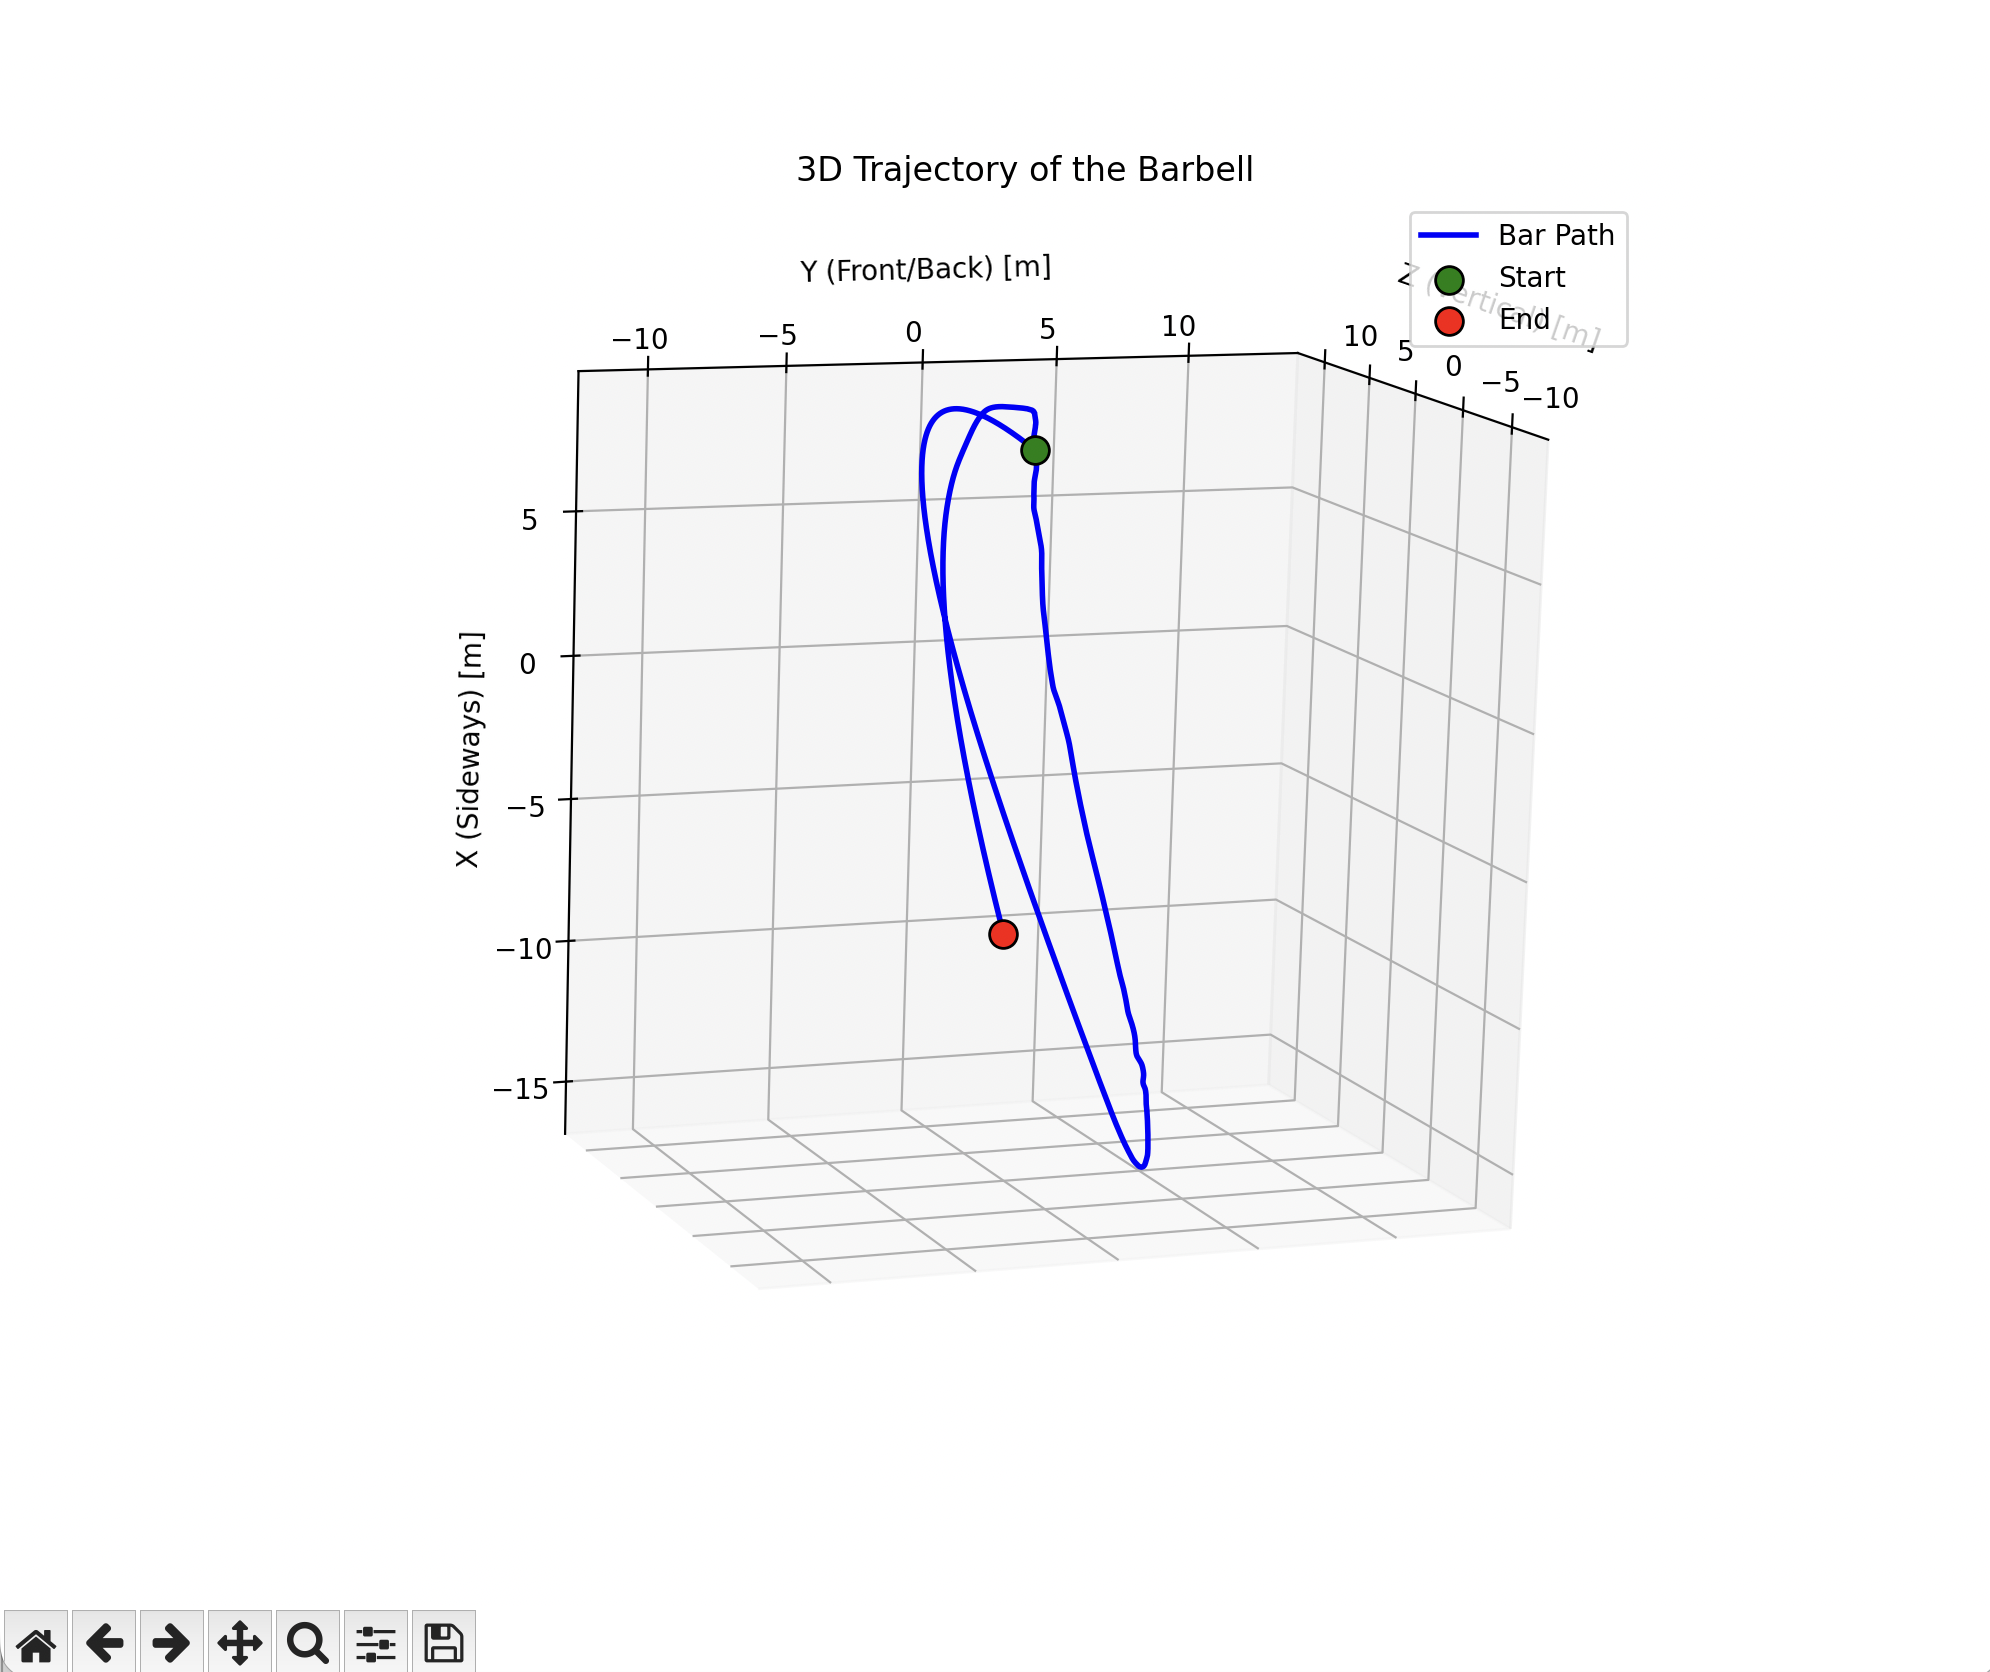
\includegraphics[width=12cm]{images/Annexes/imu-trajectory.png}
  \caption{Trajectoire 3D de la barre reconstruite par double intégration de l'accélération IMU sur un mouvement de squat.}
  \label{fig:imu-trajectory}
\end{figure}

\section*{Difficultés rencontrées}

L'approche IMU s'est heurtée à trois difficultés majeures, qui ont finalement motivé le basculement vers une approche basée sur la vision par ordinateur.

\paragraph{Calibration.}
La calibration du capteur s'est révélée laborieuse et peu reproductible entre les différentes sessions. Chaque mise en service nécessitait une procédure manuelle de calibration du magnétomètre (rotations dans les trois axes) et de l'accéléromètre (positionnement statique selon plusieurs orientations). La présence de métal dans l'environnement (rack, disques, barre elle-même) perturbait significativement les mesures du magnétomètre, rendant l'orientation absolue peu fiable malgré la compensation de biais implémentée.

\paragraph{Dérive.}
Le calcul de la vitesse et de la trajectoire par intégration de l'accélération est intrinsèquement sujet à une dérive cumulative : la moindre erreur résiduelle de calibration s'accumule au cours du temps. Bien que \texttt{scipy.signal.detrend} atténue partiellement ce phénomène en supprimant la composante linéaire de la dérive, les erreurs non linéaires persistent (figure~\ref{fig:imu-dashboard}) et produisent des trajectoires qui s'éloignent progressivement de la réalité sur des séries de plusieurs répétitions consécutives, rendant l'analyse multi-répétitions inexploitable.

\begin{figure}[h]
  \centering
  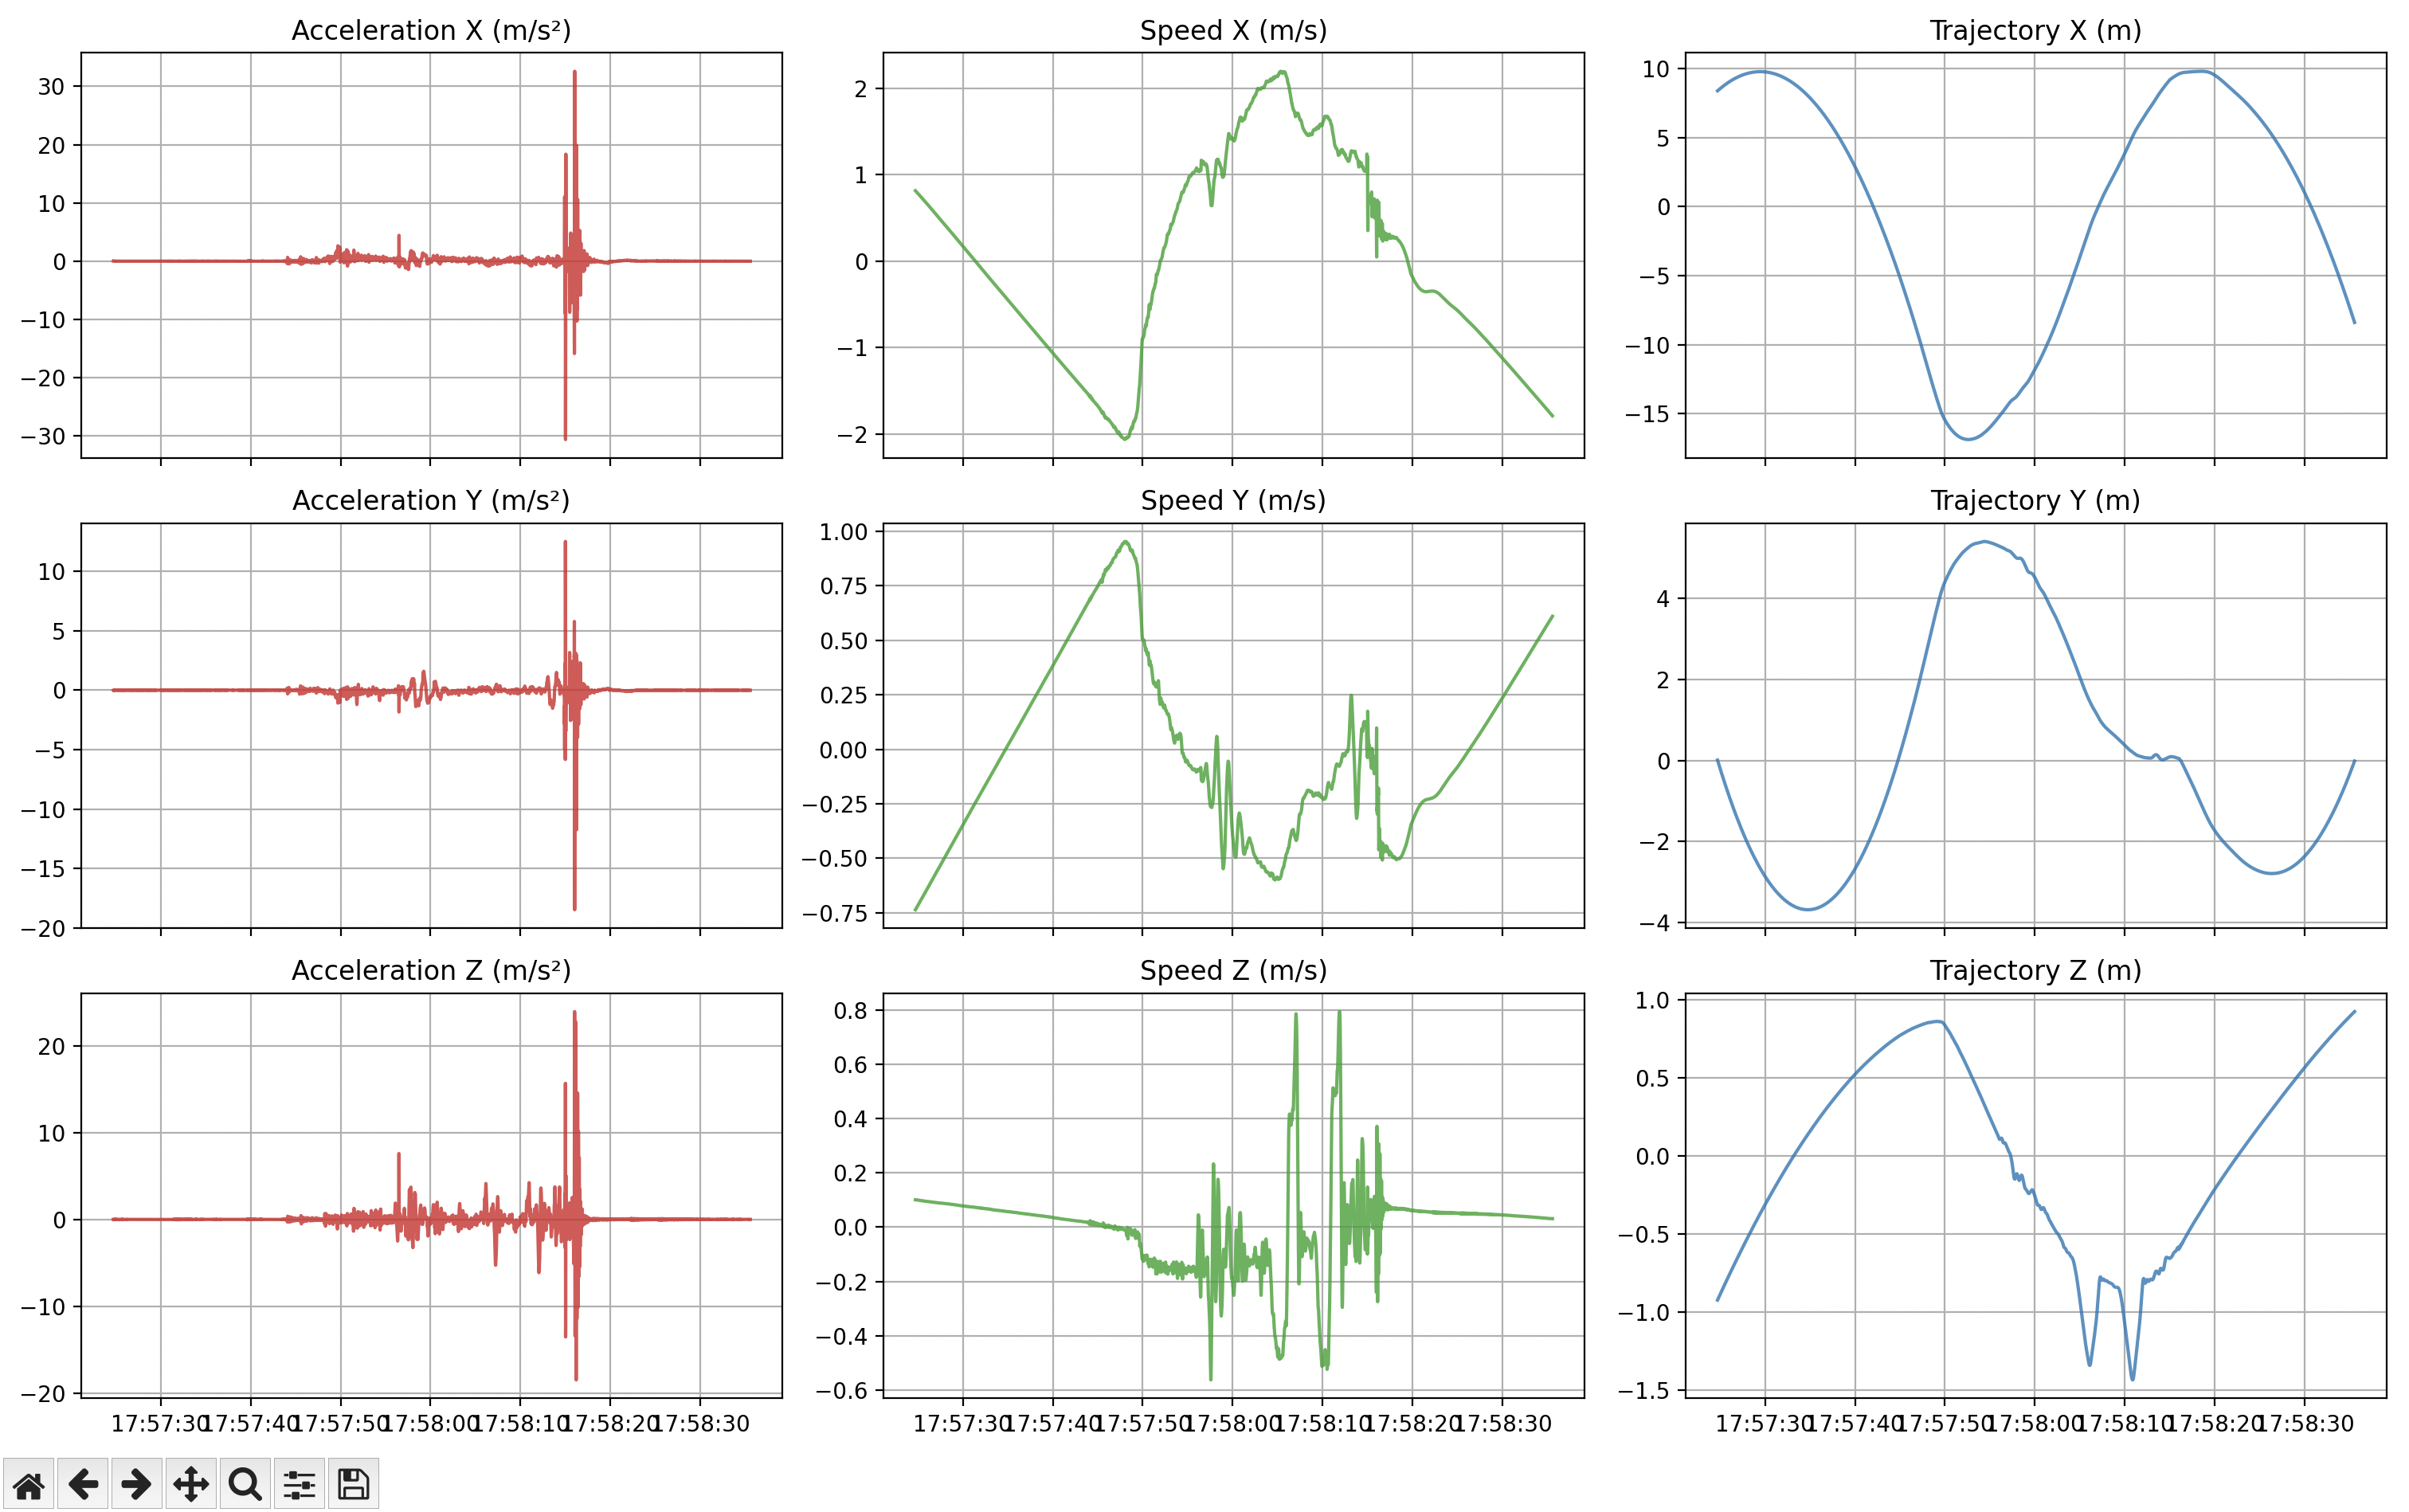
\includegraphics[width=12cm]{images/Annexes/imu-dashboard.png}
  \caption{Dashboard des données IMU : accélération, vitesse et trajectoire par axe (X, Y, Z) sur un enregistrement de squat.}
  \label{fig:imu-dashboard}
\end{figure}

\paragraph{Bruit.}
Les vibrations transmises à la barre durant les phases de mise en place et les micro-tremblements de l'individu généraient un bruit haute fréquence sur l'accéléromètre (figure~\ref{fig:imu-dashboard}). Un filtrage passe-bas atténuait ce bruit mais introduisait un lissage des pics caractéristiques du mouvement, dégradant la précision de détection des transitions de phase du mouvement.

\section*{Bilan}

Bien que l'IMU offre un accès direct aux paramètres cinématiques de la barre, son utilisation pratique en conditions d'entraînement s'est révélée trop contraignante : calibration fastidieuse à chaque session, dérive cumulative limitant la durée d'enregistrement exploitable, et bruit nécessitant un filtrage qui dégrade les transitions de phase. Surtout, l'IMU ne fournit aucune information sur la \emph{posture} de l'individu, qui constitue pourtant l'objet central de l'analyse biomécanique en force athlétique. Ces constats ont conduit à abandonner l'approche instrumentale au profit d'une approche \emph{markerless} basée sur la vision par ordinateur, capable de capturer simultanément la cinématique de la barre (via les keypoints des poignets) et la posture complète de l'individu depuis une simple caméra.


% ===============================================
% ANNEXE B
% ===============================================
\chapter{Interface web de visualisation} \label{ann:web-interface}

Cette annexe présente les fonctionnalités de l'interface web
développée pour explorer les reconstructions 3D produites par
le pipeline.

\section*{Vue d'ensemble}

L'interface se compose de trois zones distinctes : la zone de visualisation 3D centrale affichant le maillage MHR de l'athlète, le panneau de contrôle en bas à droite permettant de naviguer trame par trame et de choisir l'angle de vue caméra, et le panneau de métriques biomécaniques en haut à droite affichant les indicateurs de conformité aux critères IPF en temps réel. Les figures~\ref{fig:web-squat}, \ref{fig:web-bench} et~\ref{fig:web-deadlift} illustrent l'interface pour chacun des trois mouvements de référence.

\section*{Métriques biomécaniques calculées}

Pour chaque mouvement, les métriques suivantes sont calculées en temps réel à partir des keypoints 3D exportés par SAM 3D Body :

\paragraph{Squat.}
Profondeur IPF (hanche sous le niveau du genou sur au moins une trame), inclinaison maximale du buste sur l'ensemble de la séquence, asymétrie maximale des hanches, distance cumulée parcourue par chaque main.

\paragraph{Développé couché.}
Verrouillage des coudes (angle épaule--coude--poignet > 160° atteint en fin de mouvement), angle minimal des coudes, symétrie des poignets, distance cumulée parcourue par chaque main.

\paragraph{Soulevé de terre.}
Verrouillage des genoux, position des épaules par rapport aux hanches sur l'axe de profondeur (critères IPF), inclinaison maximale du buste, asymétrie maximale des hanches, angle minimal des hanches, distance cumulée parcourue par chaque main.

\section*{Captures d'écran représentatives}

\begin{figure}[H]
  \centering
  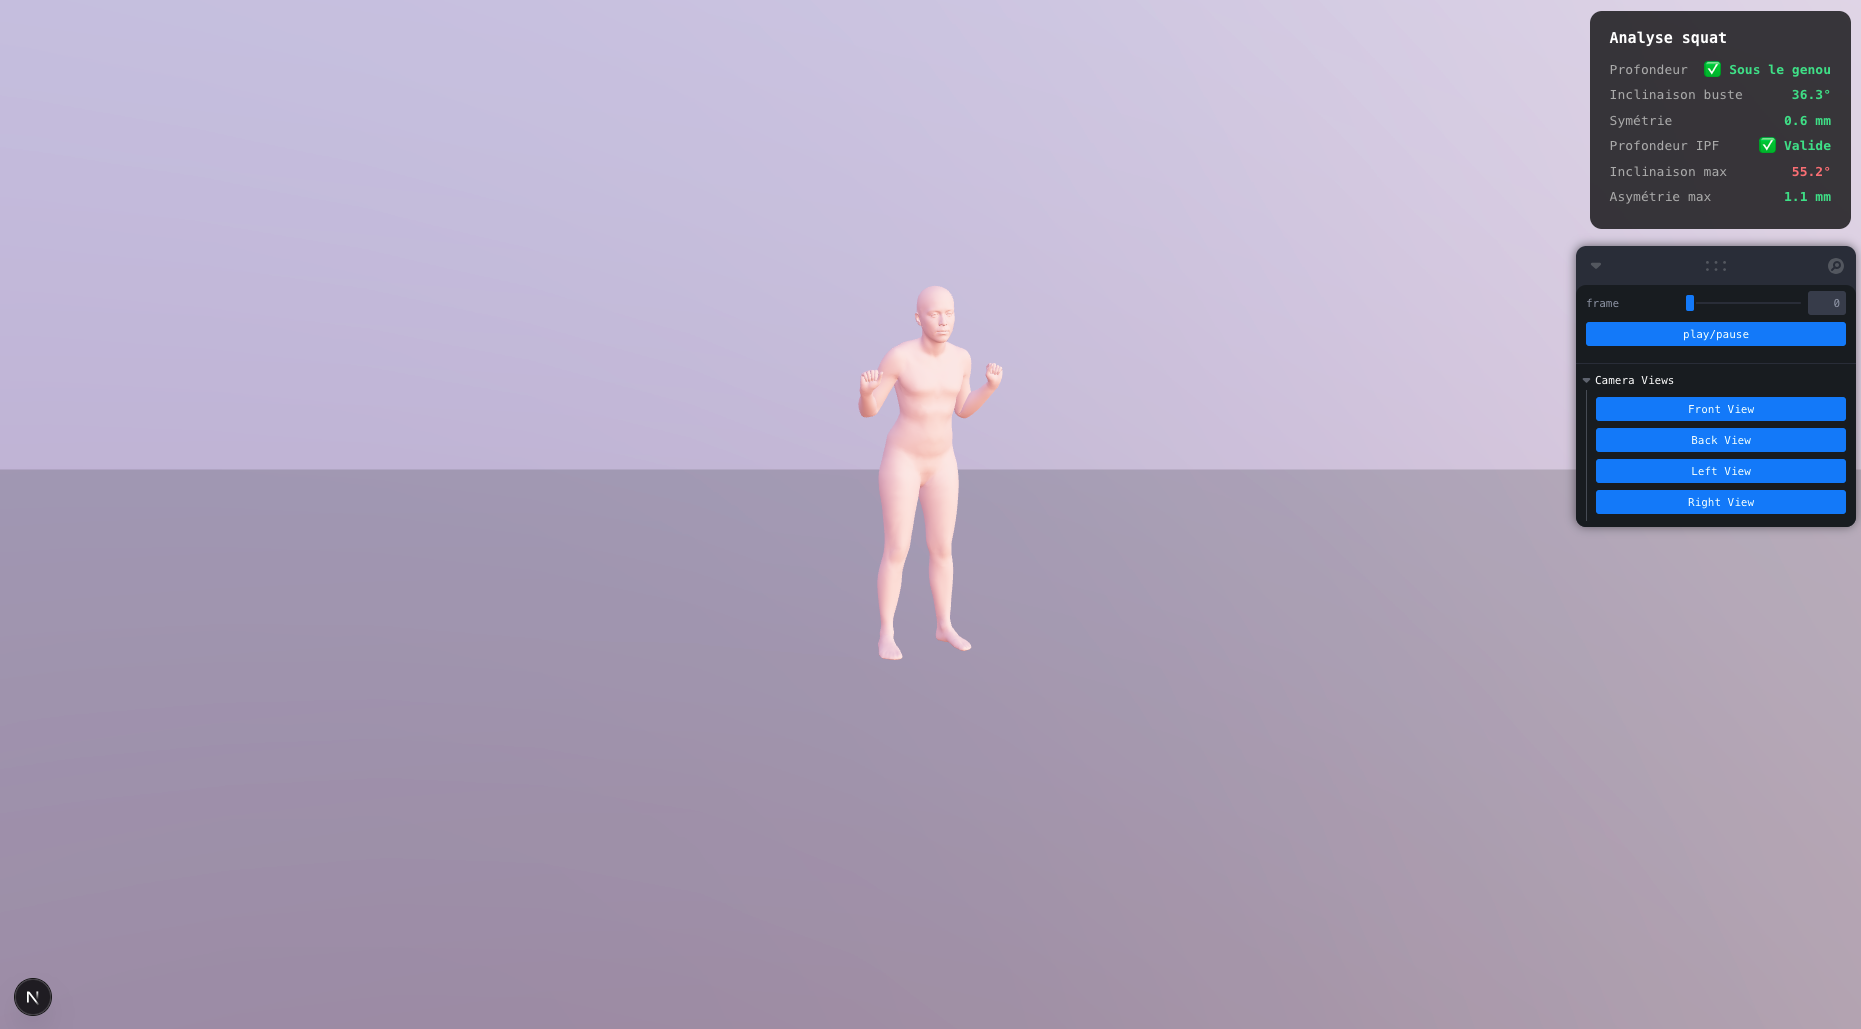
\includegraphics[width=0.95\textwidth]{images/Annexes/web_overview_squat.png}
  \caption{Interface web - squat. La profondeur IPF est validée (hanche sous le genou). L'inclinaison du buste est de 36,3° sur la trame courante, avec un maximum de 55,2° sur l'ensemble de la séquence.}
  \label{fig:web-squat}
\end{figure}

\begin{figure}[H]
  \centering
  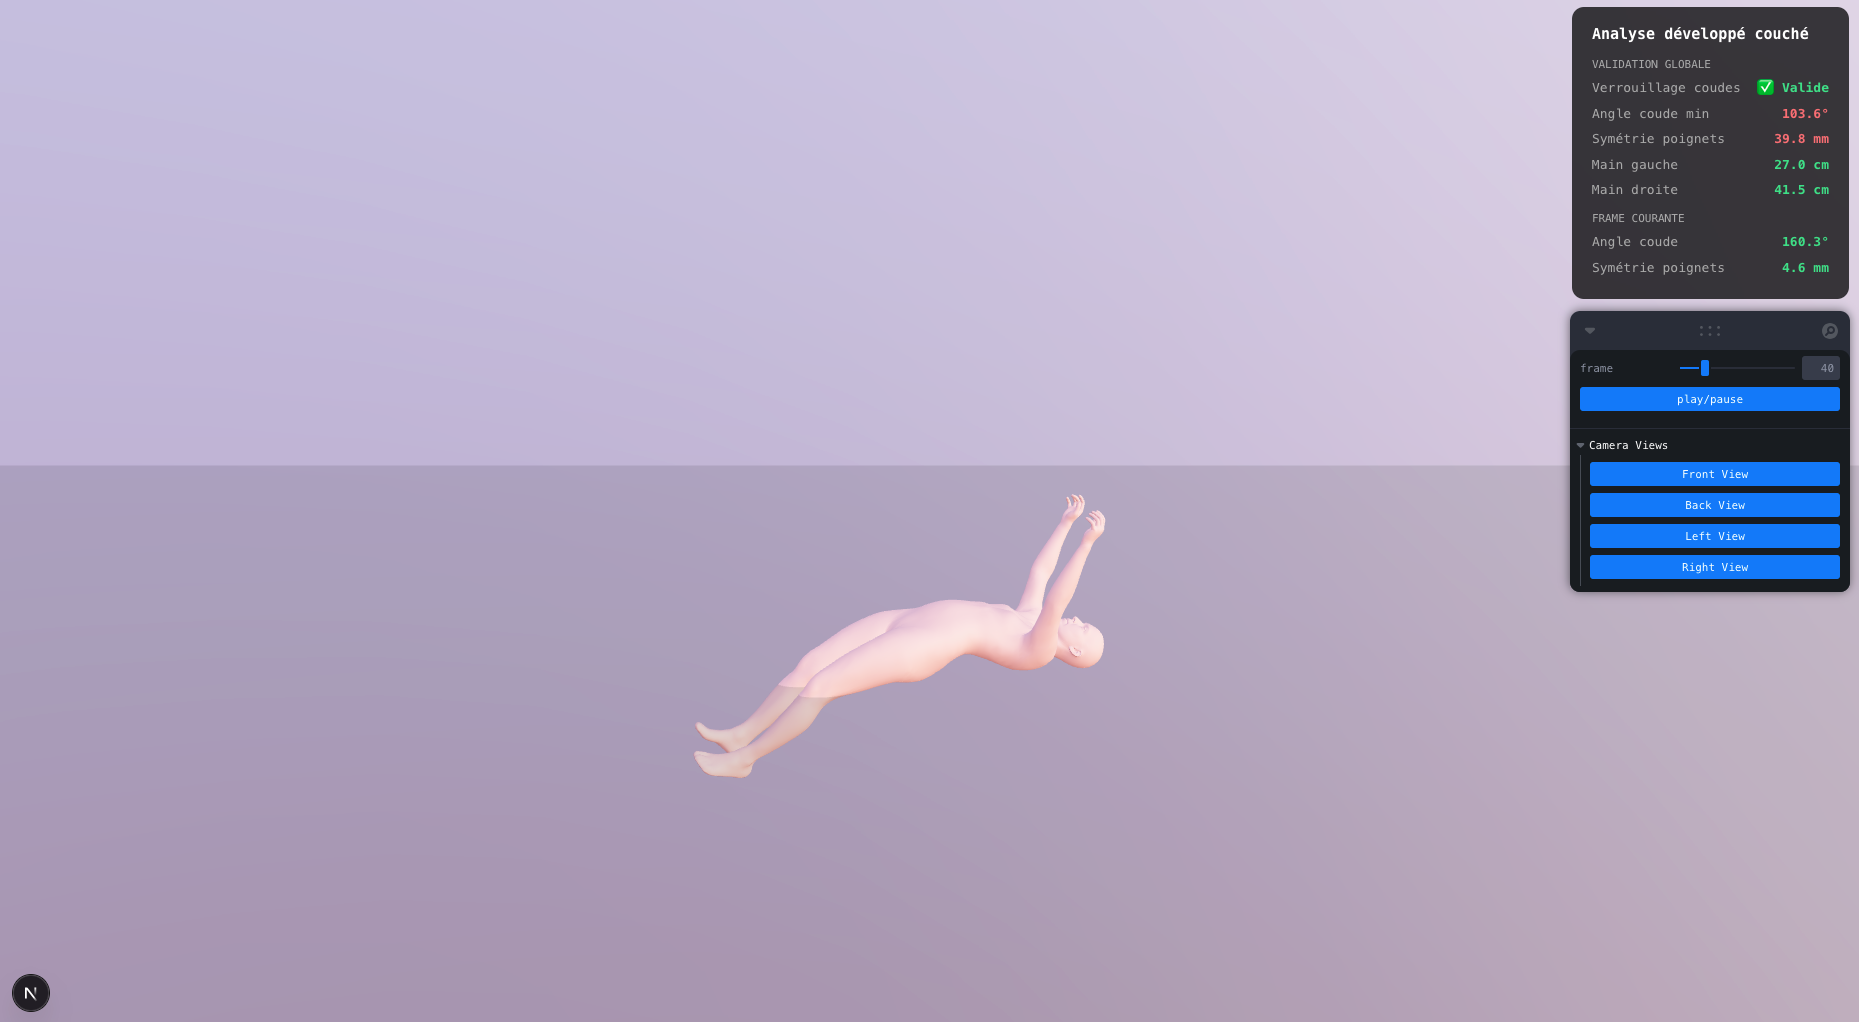
\includegraphics[width=0.95\textwidth]{images/Annexes/web_overview_bench.png}
  \caption{Interface web - développé couché. Le verrouillage des coudes est validé (angle de 160,3° atteint en fin de mouvement). L'angle minimal des coudes de 103,6° correspond à la descente de la barre.}
  \label{fig:web-bench}
\end{figure}

\begin{figure}[H]
  \centering
  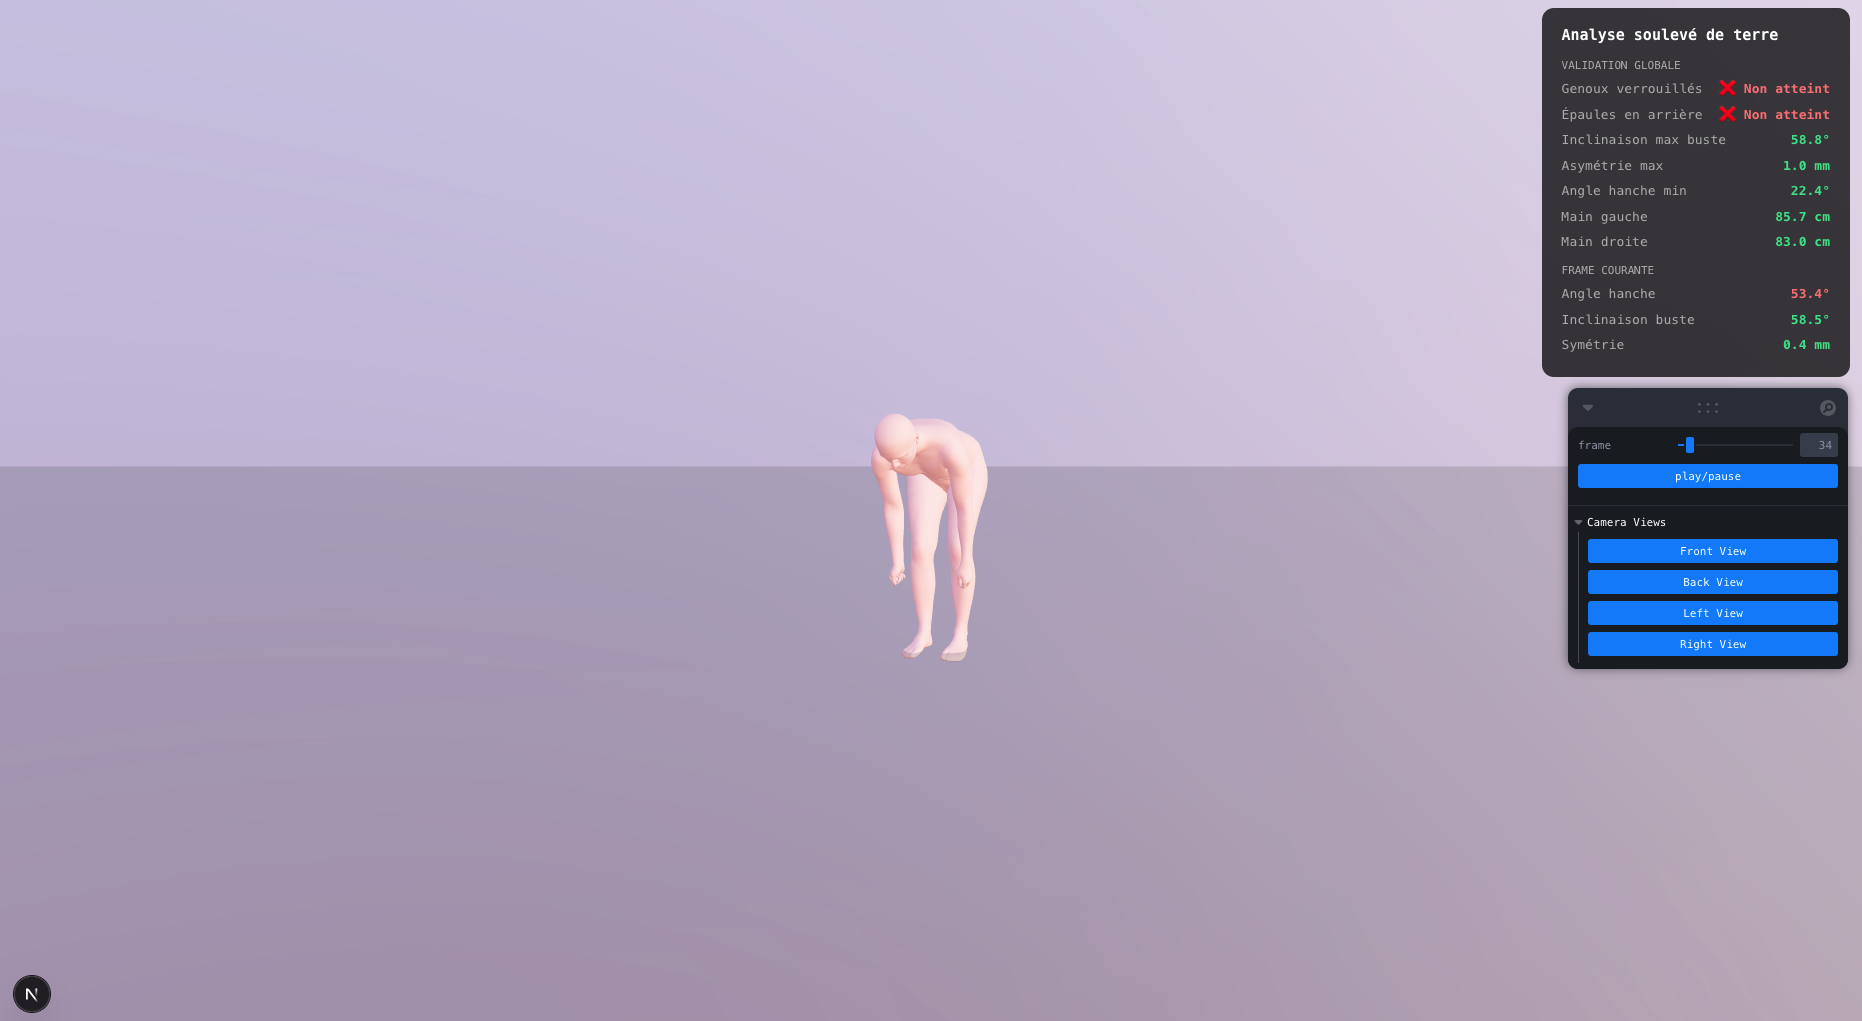
\includegraphics[width=0.95\textwidth]{images/Annexes/web_overview_deadlift.png}
  \caption{Interface web - soulevé de terre. Les critères IPF de verrouillage des genoux et d'épaules en arrière ne sont pas atteints sur cette trame, correspondant à la phase de tirage avec une inclinaison du buste de 58,5°.}
  \label{fig:web-deadlift}
\end{figure}


% ===============================================
% ANNEXE C
% ===============================================
\chapter{Composition détaillée du dataset} \label{ann:dataset-details}

Cette annexe présente la composition détaillée du dataset constitué
pour le fine-tuning de TACO.

\section*{Vidéos sources}

Le tableau~\ref{tab:dataset-detail} recense l'ensemble des vidéos
sources avec leurs métadonnées.

\begin{table}[h]
  \centering
  \small
  \begin{tabular}{llllllll}
    \hline
    \textbf{ID} & \textbf{Sujet} & \textbf{Exercice} & \textbf{Résolution} & \textbf{Durée (s)} & \textbf{FPS} & \textbf{Partition} \\
    \hline
    IMG\_0001 & S01 & Squat    & 540x720 & 2.5 & 30 & Train \\
    IMG\_0002 & S01 & Deadlift & 360x480 & 4.4 & 30 & Train \\
    IMG\_0003 & S01 & Bench    & 360x480 & 2.5 & 30 & Train \\
    IMG\_0004 & S02 & Squat    & 360x480 & 4.6 & 30 & Train \\
    IMG\_0005 & S02 & Deadlift & 360x480 & 7.5 & 30 & Val   \\
    IMG\_0006 & S02 & Deadlift & 360x480 & 3.1 & 30 & Val   \\
    IMG\_0007 & S03 & Deadlift & 540x960 & 13.3 & 30 & Train \\
    IMG\_0008 & S03 & Bench    & 360x640 & 13.4 & 30 & Val   \\
    IMG\_0009 & S03 & Bench    & 540x960 & 11.1 & 30 & Exclu (occlusion réelle) \\
    IMG\_0010 & S04 & Squat    & 3840x2160 & 13.2 & 25 & Train \\
    IMG\_0011 & S03 & Squat    & 3840x2160 & 27.1 & 25 & Exclu (occlusion réelle) \\
    IMG\_0012 & S04 & Deadlift & 3840x2160 & 24.7 & 25 & Train \\
    IMG\_0013 & S04 & Deadlift & 3840x2160 & 23.5 & 25 & Train \\
    IMG\_0014 & S04 & Bench    & 3840x2160 & 16.6 & 25 & Train \\
    IMG\_0015 & S05 & Squat    & 1280x720 & 21.2 & 30 & Train \\
    IMG\_0016 & S05 & Squat    & 1280x720 & 23.5 & 30 & Train \\
    IMG\_0017 & S05 & Deadlift & 1280x720 & 24.3 & 30 & Train \\
    IMG\_0018 & S05 & Deadlift & 1280x720 & 18.8 & 30 & Train \\
    IMG\_0019 & S06 & Deadlift & 540x960 & 8.8 & 30 & Val   \\
    IMG\_0020 & S07 & Squat    & 540x960 & 6.7 & 30 & Train \\
    IMG\_0021 & S07 & Deadlift & 360x640 & 8.4 & 30 & Train \\
    IMG\_0022 & S07 & Bench    & 360x640 & 10.5 & 30 & Train \\
    IMG\_0023 & S08 & Deadlift & 360x640 & 18.0 & 29.776 & Train \\
    IMG\_0024 & S08 & Squat    & 360x640 & 16.1 & 29.737 & Train \\
    IMG\_0025 & S08 & Bench    & 360x640 & 12.4 & 29.752 & Train \\
    \hline
    IMG\_0026 & S09 & Squat    & 536x954 & 17.7 & 30 & Test  \\
    IMG\_0027 & S09 & Bench    & 356x634 & 15.3 & 30 & Test  \\
    IMG\_0028 & S09 & Deadlift & 360x640 & 7.0 & 30 & Test  \\
    \hline
    IMG\_0098 & S03 & Squat    & 2922x1644 & 6.6 & 25 & Exclu (occlusion réelle) \\
    IMG\_0099 & S03 & Deadlift & 3840x2160 & 4.3 & 25 & Exclu (occlusion réelle) \\
    \hline
  \end{tabular}
  \caption{Composition du dataset : métadonnées des vidéos sources. Les vidéos du jeu de données de test (S09) ont été reçues après la réalisation du fine-tuning et n'apparaissent pas dans les partitions d'entraînement ou de validation.}
  \label{tab:dataset-detail}
\end{table}

\section*{Distribution par mouvement et par sujet}

La figure~\ref{fig:dataset-distribution} présente la distribution des séquences d'entraînement par mouvement et par sujet.

\begin{figure}[ht]
  \centering
  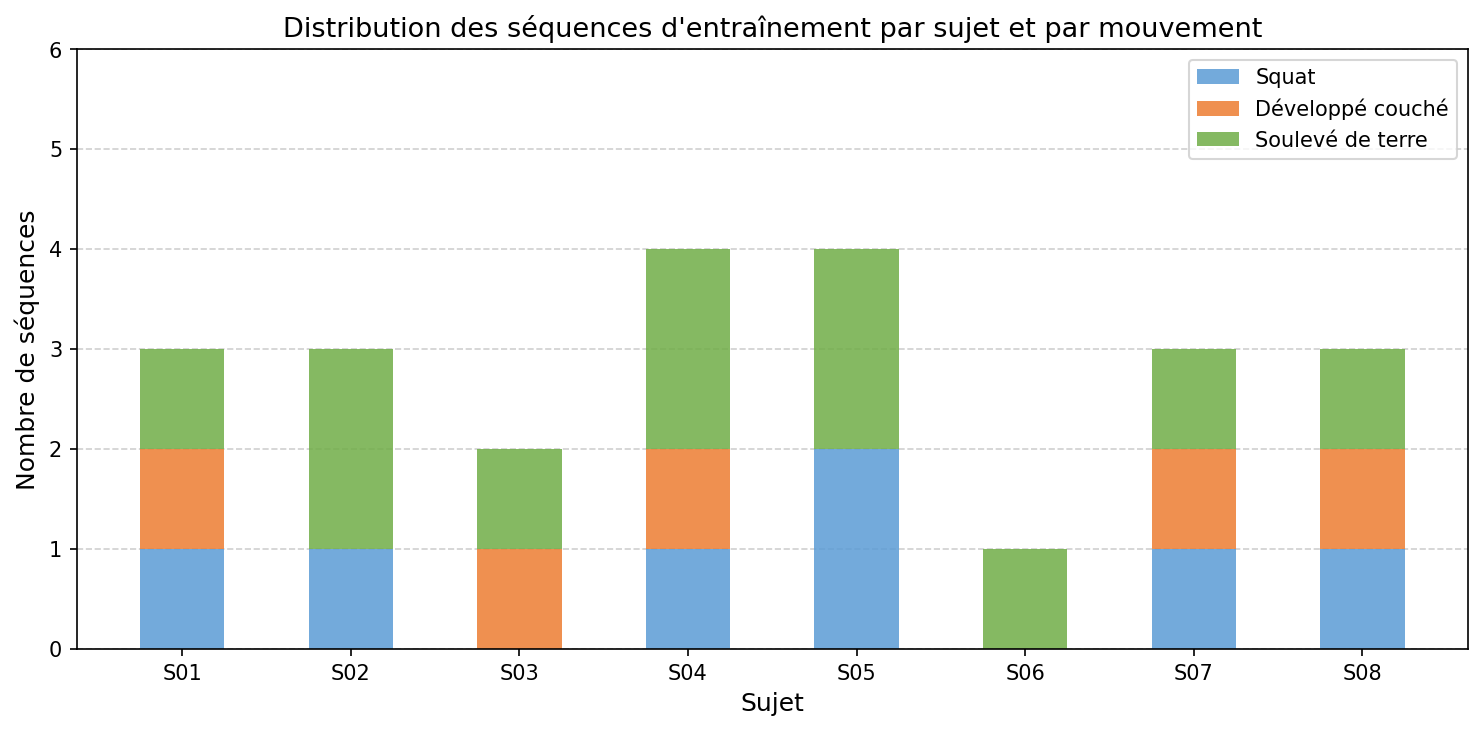
\includegraphics[width=12cm]{images/Annexes/dataset_distribution.png}
  \caption{Distribution des séquences du dataset d'entraînement par mouvement et par sujet.}
  \label{fig:dataset-distribution}
\end{figure}

\section*{Banque d'occlusions synthétiques}

La figure~\ref{fig:occluders-bank} présente l'ensemble des occlusions utilisées pour la génération synthétique des occlusions du dataset d'entraînement.

\begin{figure}[ht]
  \centering
  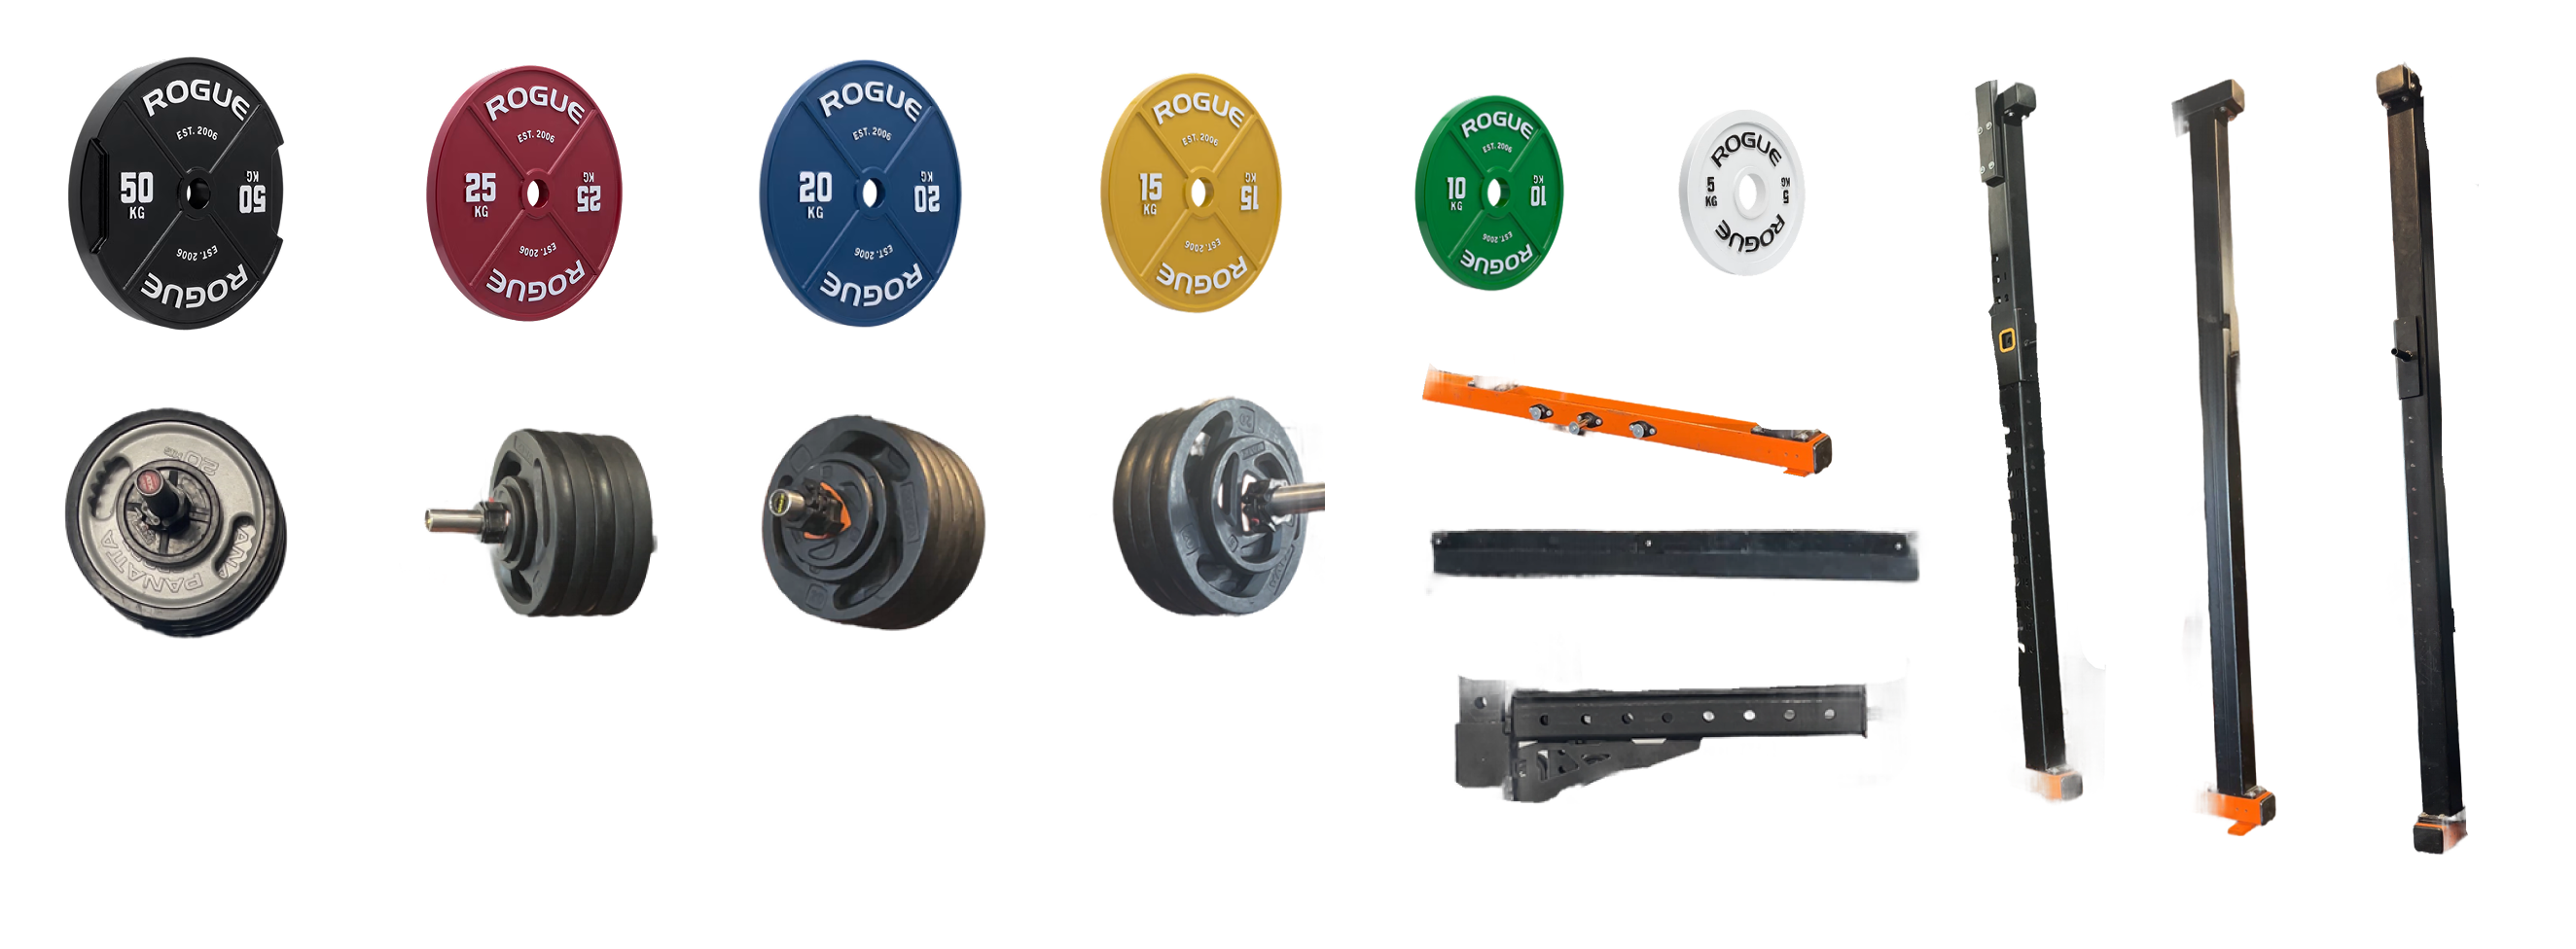
\includegraphics[width=14cm]{images/Annexes/occluders.png}
  \caption{Banque d'occlusions synthétiques utilisés pour la génération des occlusions du dataset de fine-tuning : disques IPF calibrés, disques de salle commerciale, configurations multi-disques et racks à squat.}
  \label{fig:occluders-bank}
\end{figure}


% ===============================================
% ANNEXE D
% ===============================================
\chapter{Charte de traitement des données personnelles} \label{ann:rgpd}

Cette annexe reproduit la charte RGPD établie pour la collecte des vidéos auprès des sujets volontaires.

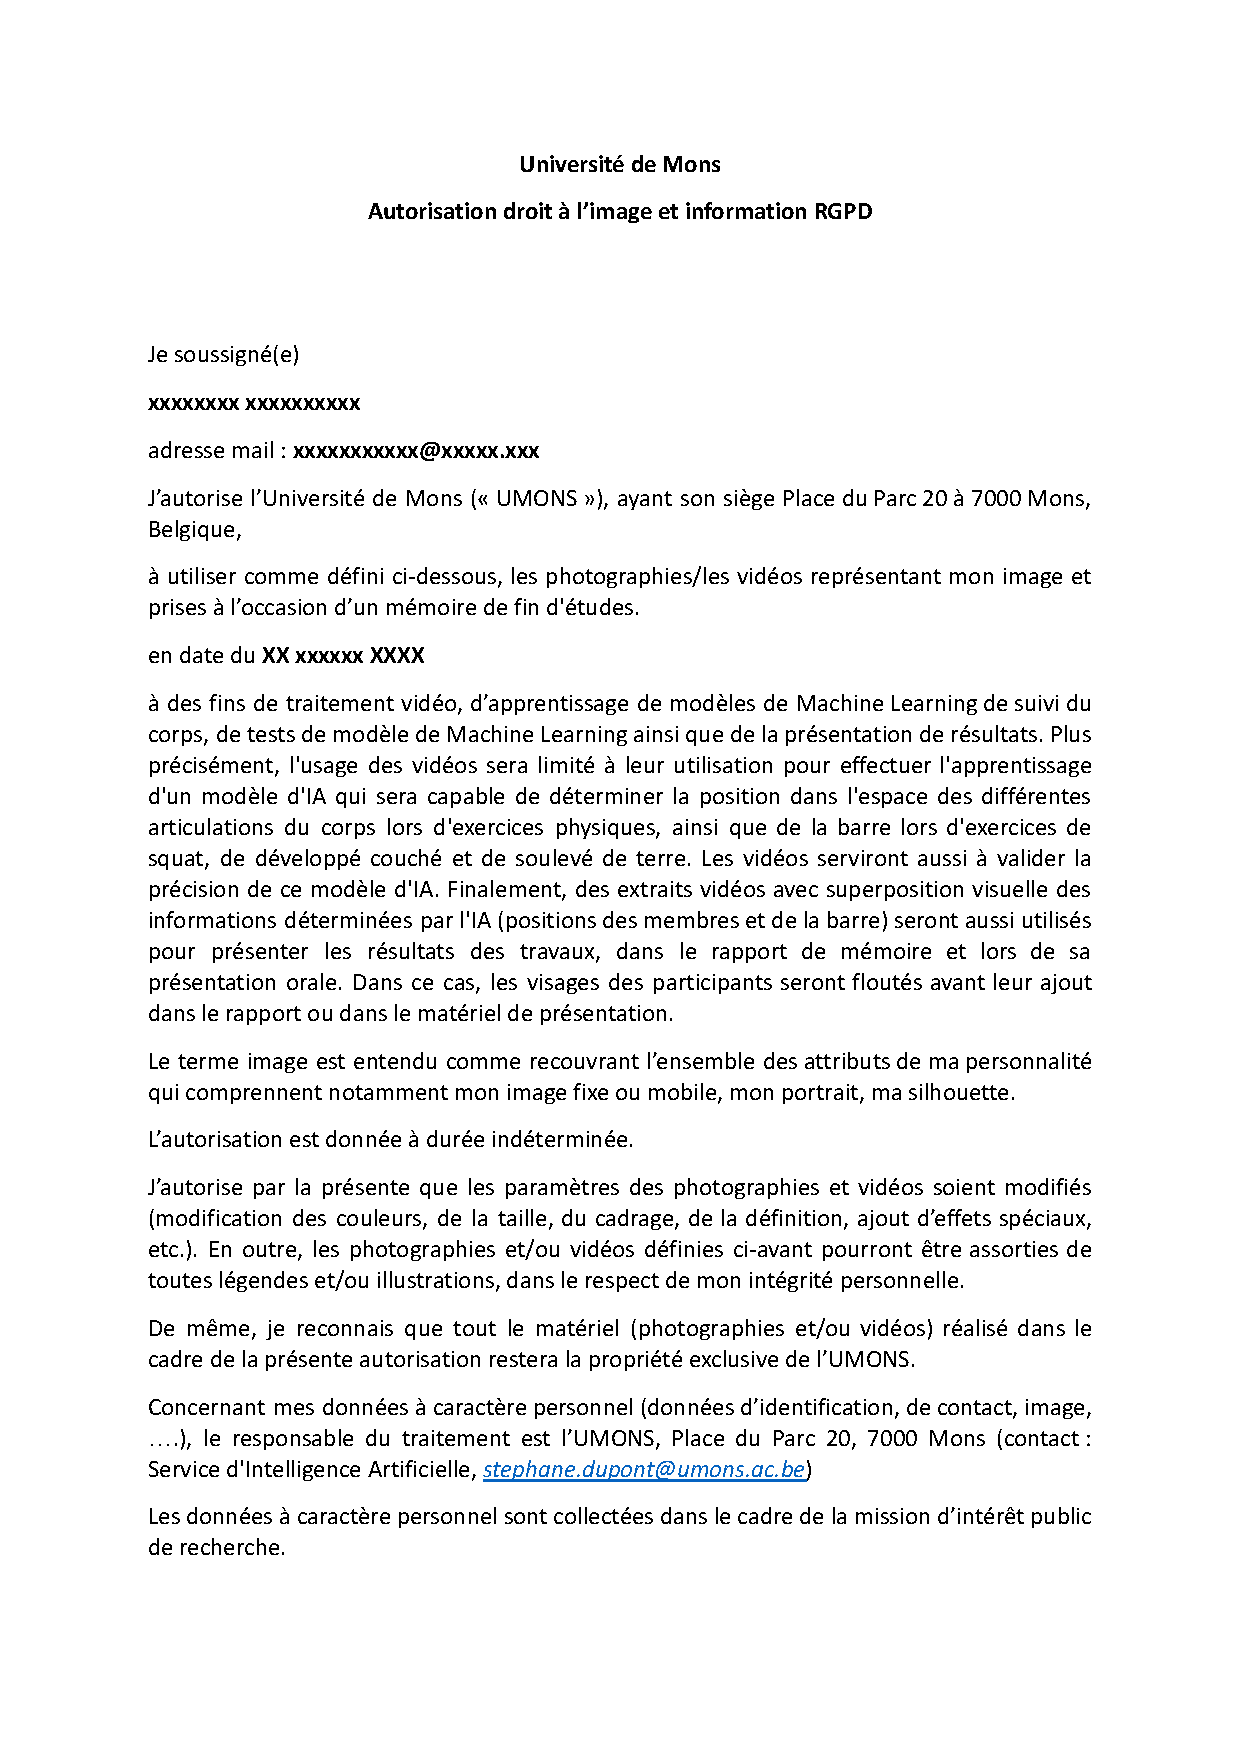
\includepdf[pages=-, scale=0.9, pagecommand={}, offset=0 -1cm]{images/Annexes/RGPD-Template.pdf}

% ===============================================
% ANNEXE E
% ===============================================
\chapter{Configuration du fine-tuning LoRA} \label{ann:lora-config}

Cette annexe détaille la configuration utilisée pour le fine-tuning LoRA de TACO, complétant les informations synthétiques fournies au chapitre~\ref{ch_four}.

\section*{Couches ciblées par LoRA}

La stratégie \texttt{time\_lora} cible 248 modules répartis en cinq catégories, tous liés au traitement temporel du UNet de Stable Video Diffusion. Le tableau~\ref{tab:lora-layers} présente une synthèse par catégorie.

\begin{table}[ht]
  \centering
  \begin{tabular}{lrrr}
    \hline
    \textbf{Type de module} & \textbf{Nb couches} &
    \textbf{Params / couche} & \textbf{Params total} \\
    \hline
    Embedding temporel (\texttt{time\_embed}) & 2
      & 25\,600 -- 40\,960 & 66\,560 \\
    Embedding de timestep (\texttt{emb\_layers}) & 22
      & 25\,600 -- 40\,960 & $\approx$ 700\,000 \\
    Position temporelle (\texttt{time\_pos\_embed}) & 24
      & 25\,600 -- 102\,400 & $\approx$ 2\,100\,000 \\
    Auto-attention temporelle (\texttt{attn1}) & 48
      & 10\,240 -- 40\,960 & $\approx$ 1\,700\,000 \\
    Cross-attention temporelle (\texttt{attn2}) & 48
      & 10\,240 -- 40\,960 & $\approx$ 1\,600\,000 \\
    Feed-forward temporel (\texttt{ff}, \texttt{ff\_in}) & 104
      & 25\,600 -- 184\,320 & $\approx$ 5\,500\,000 \\
    \hline
    \textbf{Total} & \textbf{248} & -- & \textbf{11\,700\,000} \\
    \hline
  \end{tabular}
  \caption{Synthèse des 248 couches ciblées par la stratégie \texttt{time\_lora} avec rang $r = 16$. Les modules d'attention spatiale, le VAE et les embeddings de conditionnement (CLIP) sont intégralement gelés et ne figurent pas dans ce tableau.}
  \label{tab:lora-layers}
\end{table}

\section*{Statistiques d'utilisation des ressources}

\begin{figure}[H]
  \centering

  % GPU Utilisation
  \begin{subfigure}[t]{0.48\textwidth}
    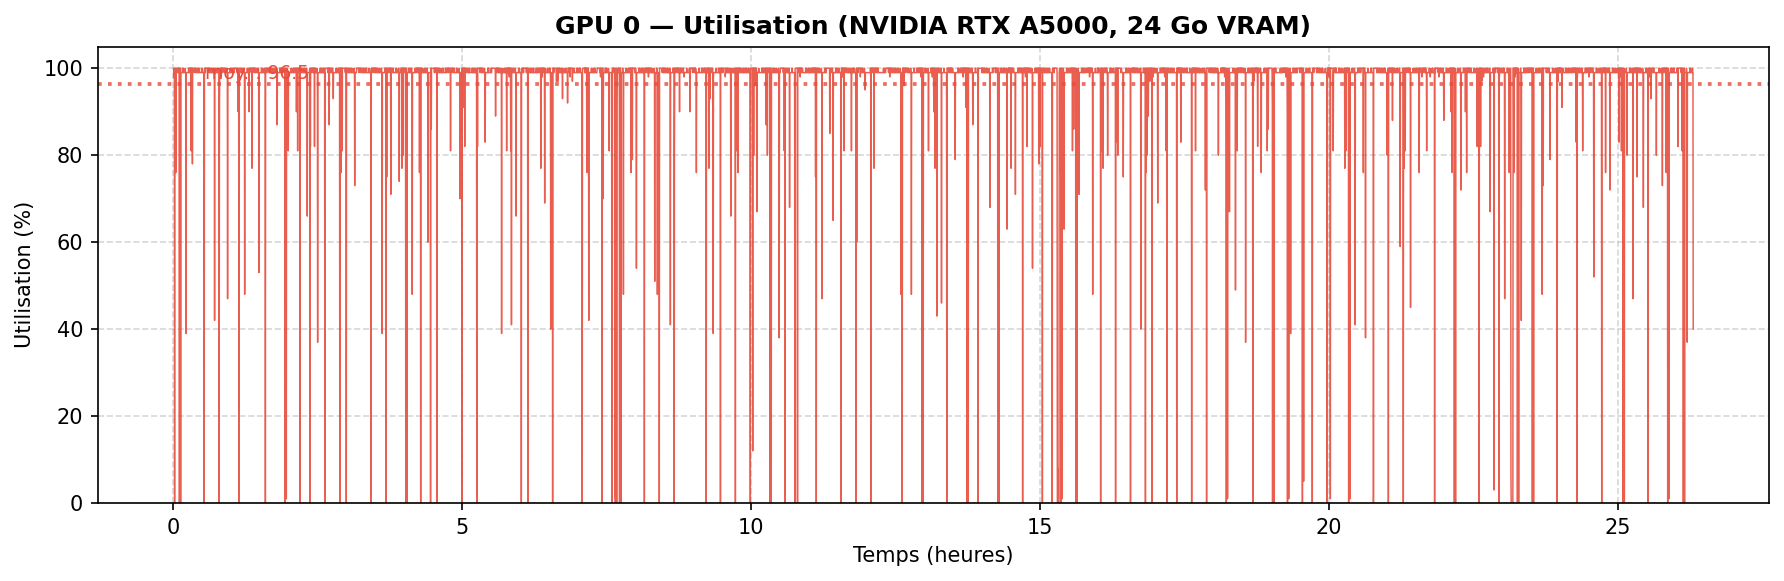
\includegraphics[width=\textwidth]{images/Annexes/gpu0_utilisation.png}
    \caption{GPU 0 — Utilisation (\%)}
  \end{subfigure}
  \hfill
  \begin{subfigure}[t]{0.48\textwidth}
    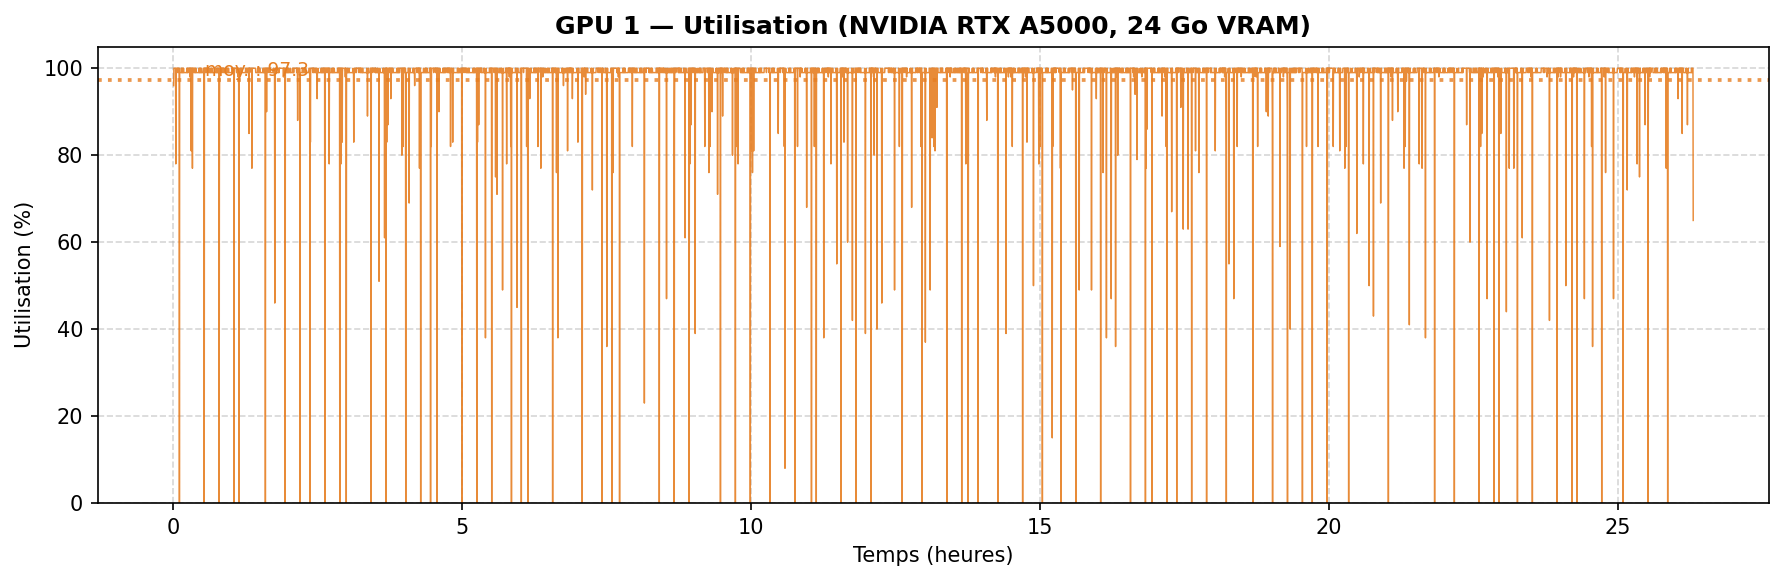
\includegraphics[width=\textwidth]{images/Annexes/gpu1_utilisation.png}
    \caption{GPU 1 — Utilisation (\%)}
  \end{subfigure}

  \vspace{0.5em}

  % GPU Température
  \begin{subfigure}[t]{0.48\textwidth}
    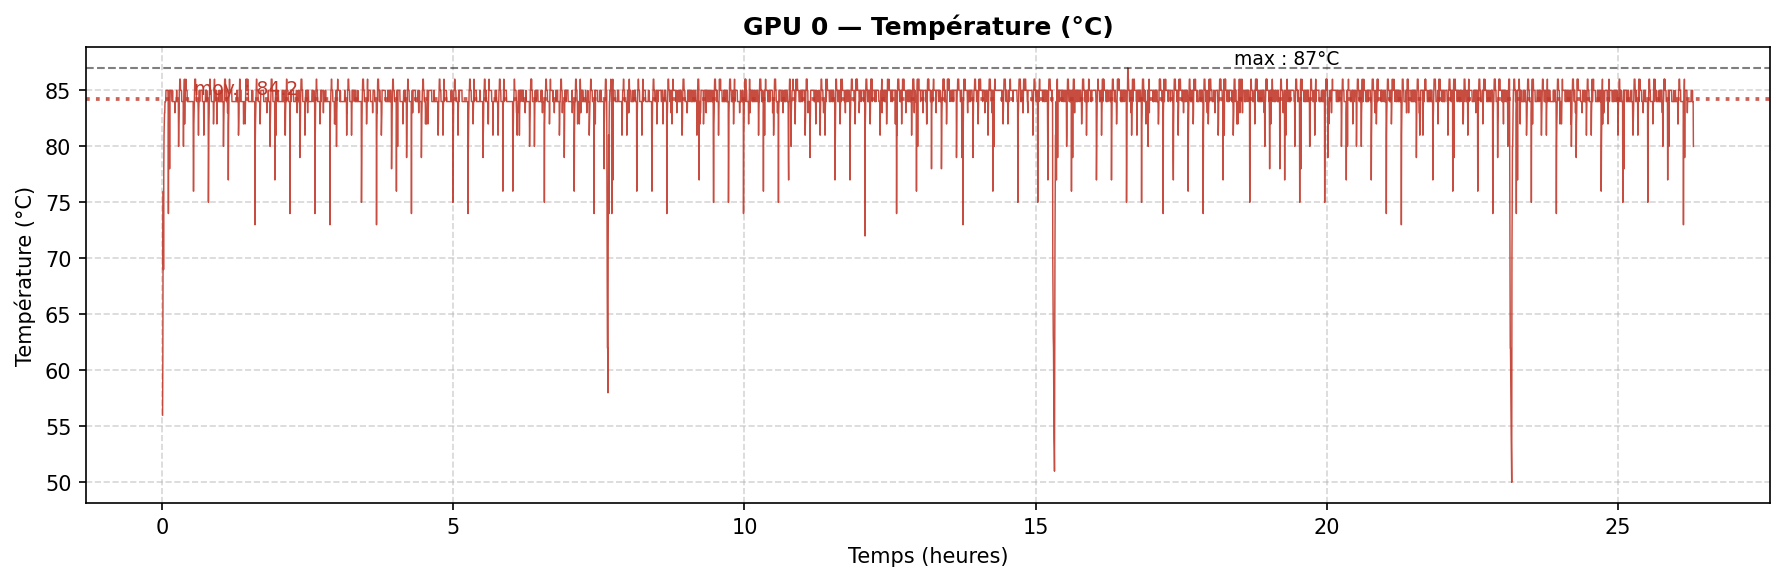
\includegraphics[width=\textwidth]{images/Annexes/gpu0_temperature.png}
    \caption{GPU 0 — Température (°C)}
  \end{subfigure}
  \hfill
  \begin{subfigure}[t]{0.48\textwidth}
    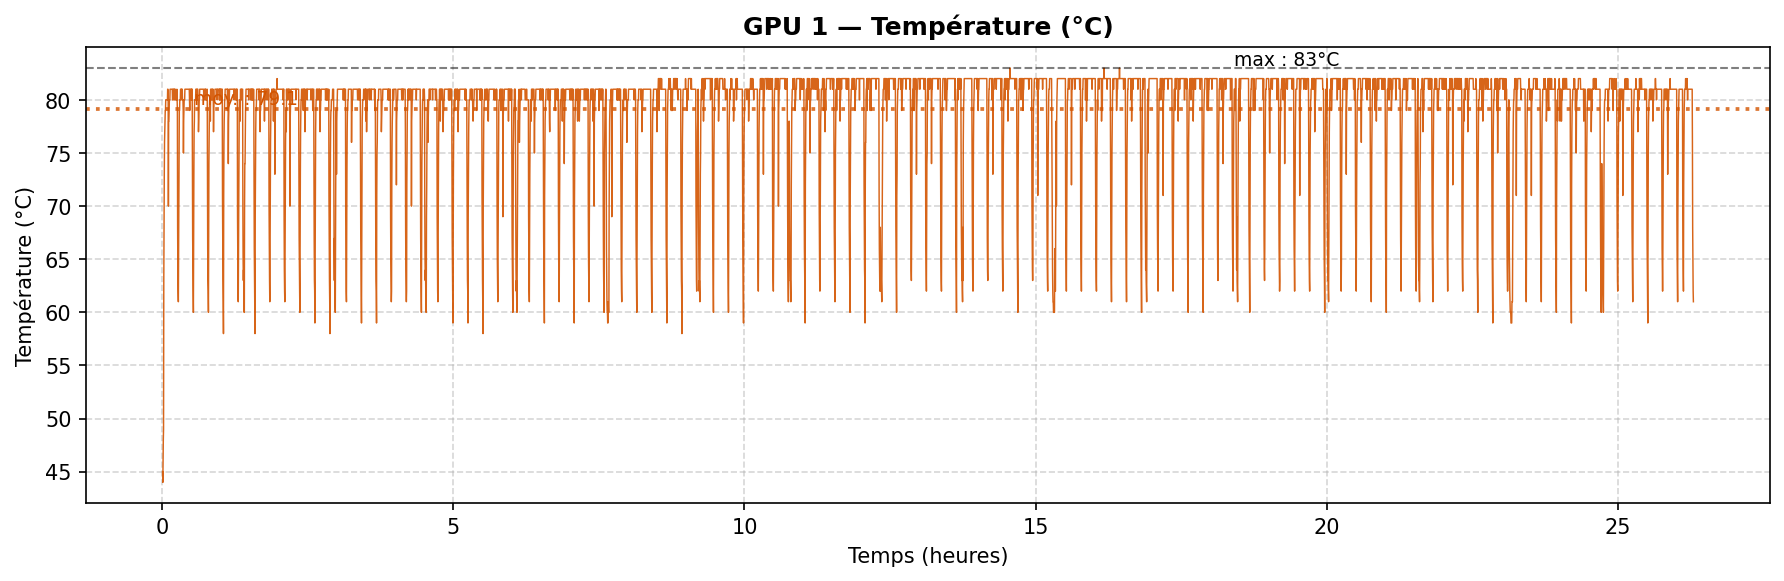
\includegraphics[width=\textwidth]{images/Annexes/gpu1_temperature.png}
    \caption{GPU 1 — Température (°C)}
  \end{subfigure}

  \vspace{0.5em}

  % RAM et CPU
  \begin{subfigure}[t]{0.48\textwidth}
    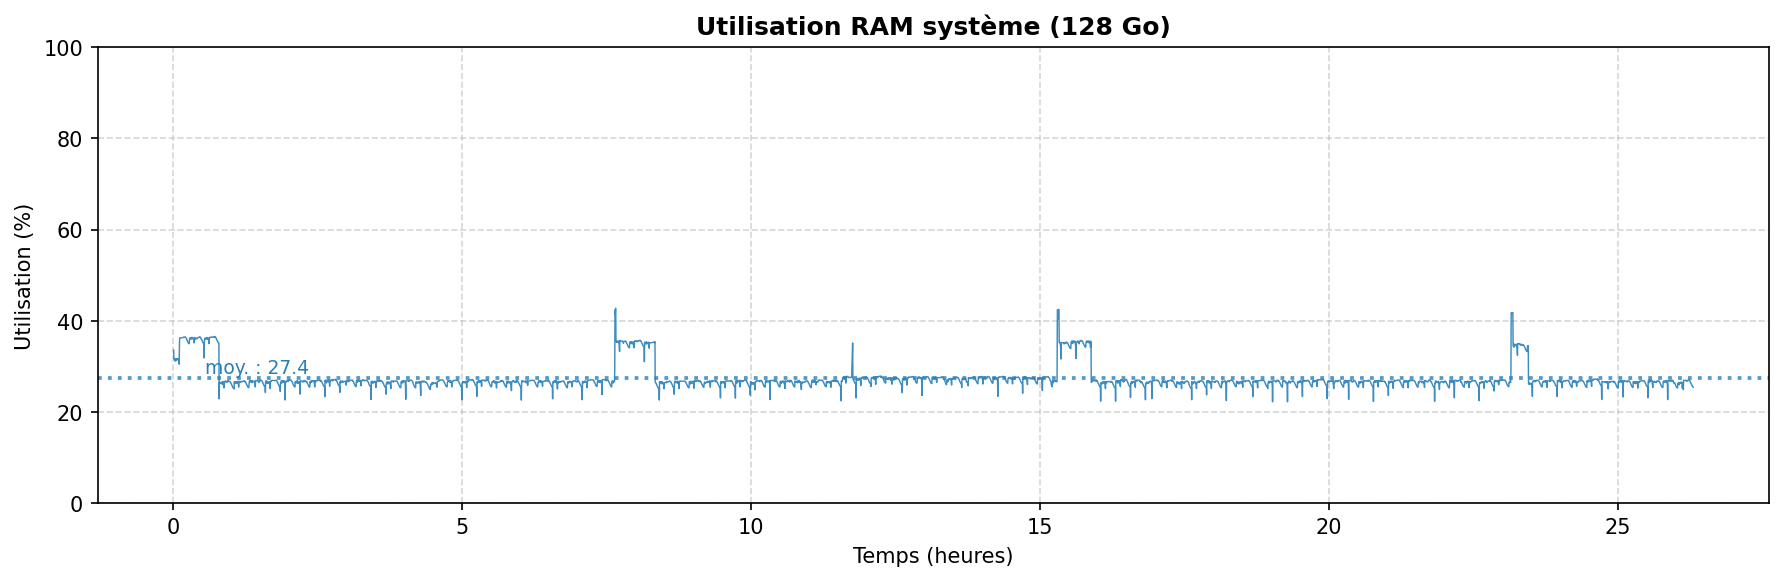
\includegraphics[width=\textwidth]{images/Annexes/ram_utilisation.png}
    \caption{Utilisation RAM système (128~Go)}
  \end{subfigure}
  \hfill
  \begin{subfigure}[t]{0.48\textwidth}
    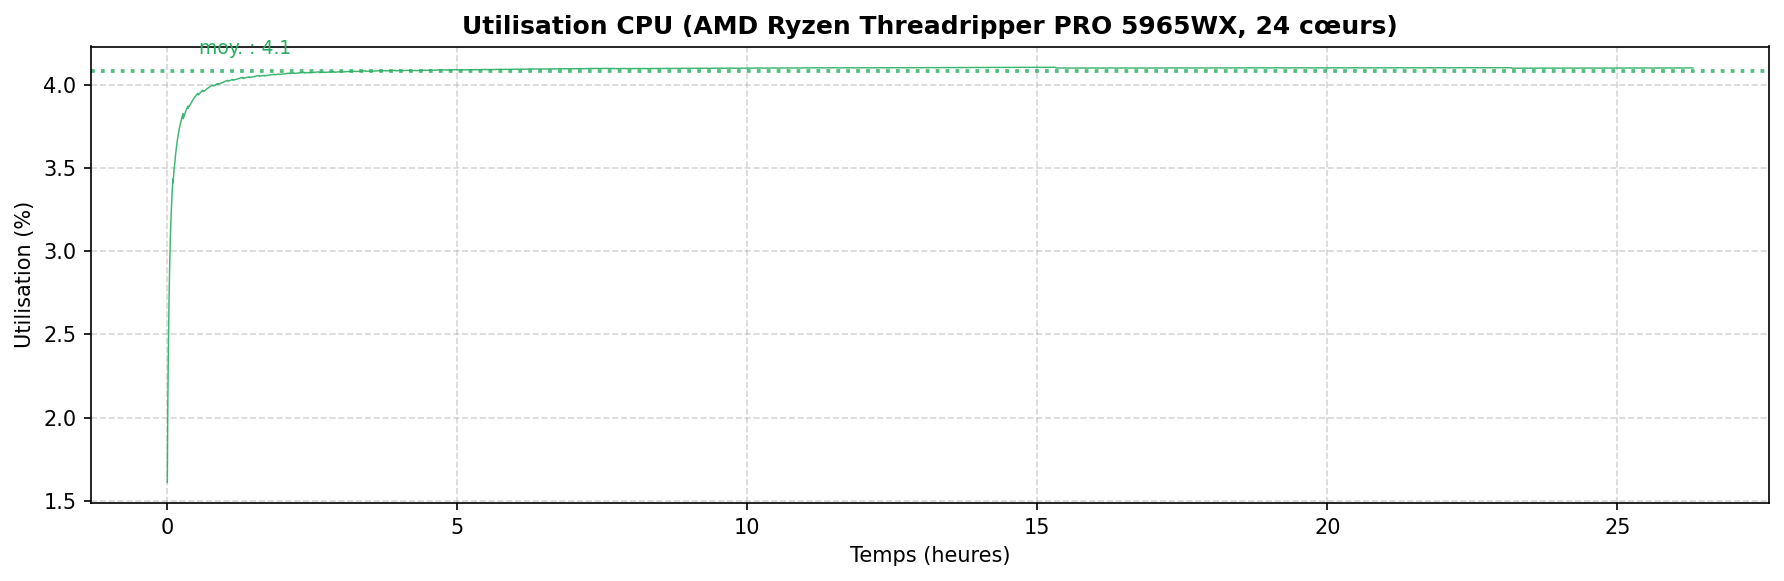
\includegraphics[width=\textwidth]{images/Annexes/cpu_utilisation.png}
    \caption{Utilisation CPU (24 cœurs)}
  \end{subfigure}

  \caption{Utilisation des ressources matérielles durant le fine-tuning LoRA sur 26,3 heures. Les deux GPU atteignent une utilisation moyenne de 96,5\,\% et 97,3\,\% respectivement, confirmant la saturation effective du matériel disponible. La RAM système reste modérément sollicitée (27,4\,\% en moyenne), le goulot d'étranglement étant la mémoire VRAM.}
  \label{fig:system-usage}
\end{figure}


% ===============================================
% ANNEXE F
% ===============================================
\chapter{Reproductibilité et code source} \label{ann:reproducibility}

\section*{Dépôt de code}

L'intégralité du code source du pipeline est disponible publiquement sur GitHub :

\begin{center}
  \url{https://github.com/nicolasdelp/MEMOIRE-Master-en-Sciences-Informatiques}

  \vspace{0.5em}
  \qrcode[height=2.5cm]{https://github.com/nicolasdelp/MEMOIRE-Master-en-Sciences-Informatiques}
  
  \vspace{0.3em}
  {\small \textit{Scanner pour accéder au dépôt GitHub}}
\end{center}

\section*{Structure du projet}

\begin{lstlisting}[style=tree]
/
|-- code/
|   |-- checkpoints/    (checkpoints des modeles)
|   |-- logs/           (logs d'entrainement)
|   |-- models/         (SAM3, MoGe, TACO, SAM 3D Body)
|   |-- scripts/        (differents scripts d'execution)
|   `-- web/            (interface de visualisation)
|-- data/
|   |-- assets/         (occlusions et ressources visuelles)
|   |-- datasets/       (dataset de fine-tuning)
|   |-- inputs/         (videos brutes)
|   `-- outputs/        (resultats intermediaires)
|-- report/
|   |-- chapters/       (chapitres LaTeX)
|   |-- images/         (figures et illustrations)
|   |-- memoire.bib     (bibliographie)
|   |-- memoire.pdf     (document compile)
|   `-- memoire.tex     (fichier principal)
|-- models.lock         (versions des checkpoints)
|-- pixi.toml           (dependances et taches)
`-- README.md
\end{lstlisting}

\section*{Instructions d'installation et d'utilisation}

L'ensemble des instructions détaillées est disponible dans le fichier \texttt{README.md} du dépôt. Les étapes principales sont résumées ci-dessous.

\paragraph{Prérequis matériels (minimum).}~\\
\begin{itemize}
  \item 2 GPU NVIDIA RTX A5000 (24~Go VRAM chacun) ou équivalent
  \item 128~Go de RAM système
  \item Ubuntu 22.04 LTS, CUDA 12.2
\end{itemize}

\paragraph{1. Téléchargement des checkpoints.}~\\

Installer l'outil CLI HuggingFace puis s'authentifier :

\begin{lstlisting}[style=bash]
curl -LsSf https://hf.co/cli/install.sh | bash
hf auth login
\end{lstlisting}

Télécharger chaque checkpoint dans son dossier dédié
(voir tableau~\ref{tab:checkpoints} pour les liens) :

\begin{lstlisting}[style=bash]
cd code/checkpoints/sam3/
hf download facebook/sam3 sam3.pt --local-dir .

cd code/checkpoints/moge/
hf download Ruicheng/moge-2-vitl model.pt --local-dir .

cd code/checkpoints/taco/
wget https://huggingface.co/datasets/JasonAplp/TACO/\
resolve/main/checkpoints/last.ckpt
hf download Nicolasdelp/TACO-LoRA-Powerlifting \
lora.ckpt --local-dir .

cd code/checkpoints/sam_3d_body/
hf download facebook/sam-3d-body-vith model.ckpt --local-dir .
curl -OL https://github.com/facebookresearch/MHR/\
releases/download/v1.0.0/assets.zip
unzip -p assets.zip assets/mhr_model.pt > mhr_model.pt
rm assets.zip
\end{lstlisting}

\paragraph{2. Installation de Pixi et du dataset.}~\\

\begin{lstlisting}[style=bash]
wget -qO- https://pixi.sh/install.sh | sh
pixi self-update
\end{lstlisting}

Télécharger et extraire le dataset :

\begin{lstlisting}[style=bash]
cd data/
for tar_file in outputs/IMG_*.tar; do
    tar -xf "$tar_file" -C outputs/
done
\end{lstlisting}

\paragraph{3. Lancer le pipeline principal.}~\\

\begin{lstlisting}[style=bash]
pixi run main-pipeline
\end{lstlisting}

\paragraph{4. Lancer l'interface web de visualisation.}~\\

Télécharger les maillages 3D précalculés :

\begin{lstlisting}[style=bash]
cd code/web/public/
hf download Nicolasdelp/Dataset-TFE-Web \
--repo-type=dataset --local-dir .
\end{lstlisting}

Installer Node.js (voir \url{https://nodejs.org/en/download}),
puis lancer l'application :

\begin{lstlisting}[style=bash]
cd code/web/
npm run dev
\end{lstlisting}

\paragraph{5. Reproduire le fine-tuning LoRA.}~\\

\begin{lstlisting}[style=bash]
cd code/models/taco/
conda env create -f environment.yml
conda activate taco
bash train_continue.sh
\end{lstlisting}

\section*{Checkpoints des modèles}

Les checkpoints des différents modèles sont hébergés séparément en raison de leur taille. Le tableau~\ref{tab:checkpoints} recense les liens de téléchargement pour chaque composant du pipeline.

\begin{table}[h]
  \centering
  \small
  \begin{tabular}{ll}
    \hline
    \textbf{Modèle / Ressource} & \textbf{Lien} \\
    \hline
    SAM3 & \url{https://huggingface.co/facebook/sam3} \\
    OpenCLIP (vocabulaire) & \url{https://huggingface.co/spaces/LanguageBind/} \\
                           & \url{LanguageBind/resolve/main/open_clip/} \\
                           & \url{bpe_simple_vocab_16e6.txt.gz} \\
    MoGe-2 & \url{https://huggingface.co/Ruicheng/moge-2-vitl} \\
    TACO baseline & \url{https://huggingface.co/datasets/JasonAplp/TACO/} \\
                  & \url{resolve/main/checkpoints/last.ckpt} \\
    TACO-LoRA-Powerlifting & \url{https://huggingface.co/Nicolasdelp/} \\
    (contribution de ce mémoire) & \url{TACO-LoRA-Powerlifting} \\
    SAM 3D Body & \url{https://huggingface.co/facebook/sam-3d-body-vith} \\
    MHR (assets) & \url{https://github.com/facebookresearch/MHR/} \\
                 & \url{releases/download/v1.0.0/assets.zip} \\
    \hline
  \end{tabular}
  \caption{Liens de téléchargement des checkpoints utilisés dans le pipeline.}
  \label{tab:checkpoints}
\end{table}

\section*{Dataset}

Le dataset constitué pour le fine-tuning de TACO est hébergé sur des disques durs à l'Université de Mons, comme indiqué dans la charte RGPD (annexe~\ref{ann:rgpd}).

\end{document}













